\documentclass{article}
\usepackage[utf8]{inputenc}
\usepackage[spanish]{babel}
\usepackage{listings}
\usepackage{subfigure}
\usepackage{graphicx}
\usepackage{url}
\usepackage{multirow}
\usepackage{color}
\usepackage{booktabs}


\setlength{\parindent}{0pt}
\setlength{\parskip}{1em}


\definecolor{mygreen}{rgb}{0,0.6,0}
\definecolor{mygray}{rgb}{0.5,0.5,0.5}
\definecolor{mymauve}{rgb}{0.58,0,0.82}
\lstset{ 
  backgroundcolor=\color{white},   % choose the background color; you must add \usepackage{color} or \usepackage{xcolor}; should come as last argument
  basicstyle=\footnotesize,        % the size of the fonts that are used for the code
  breakatwhitespace=false,         % sets if automatic breaks should only happen at whitespace
  breaklines=true,                 % sets automatic line breaking
  captionpos=b,                    % sets the caption-position to bottom
  commentstyle=\color{mygreen},    % comment style
  deletekeywords={...},            % if you want to delete keywords from the given language
  escapeinside={\%}{)},          % if you want to add LaTeX within your code
  extendedchars=true,              % lets you use non-ASCII characters; for 8-bits encodings only, does not work with UTF-8
  firstnumber=1,                % start line enumeration with line 1000
  frame=single,	                   % adds a frame around the code
  keepspaces=true,                 % keeps spaces in text, useful for keeping indentation of code (possibly needs columns=flexible)
  keywordstyle=\color{blue},       % keyword style
  language=Octave,                 % the language of the code
  morekeywords={*,...},            % if you want to add more keywords to the set
  numbers=left,                    % where to put the line-numbers; possible values are (none, left, right)
  numbersep=5pt,                   % how far the line-numbers are from the code
  numberstyle=\tiny\color{mygray}, % the style that is used for the line-numbers
  rulecolor=\color{black},         % if not set, the frame-color may be changed on line-breaks within not-black text (e.g. comments (green here))
  showspaces=false,                % show spaces everywhere adding particular underscores; it overrides 'showstringspaces'
  showstringspaces=false,          % underline spaces within strings only
  showtabs=false,                  % show tabs within strings adding particular underscores
  stepnumber=1,                    % the step between two line-numbers. If it's 1, each line will be numbered
  stringstyle=\color{mymauve},     % string literal style
  tabsize=2,	                   % sets default tabsize to 2 spaces
  title=\lstname                  % show the filename of files included with \lstinputlisting; also try caption instead of title
}
\title{Tarea 5}

\author{5271}
\date{\today}

\begin{document}
\maketitle

\section{Algoritmo generador de grafos}

Gracias a la versatilidad de Los grafos como modelo de representación de datos, los procesos aleatorios de generación de grafos también son relevantes en aplicaciones que van desde la física, biología a la sociología \cite{Nobari}.

Otra de las aplicaciones de los grafos de generación aleatoria es en la representación de una red telefónica donde los vértices son centrales telefónicas, las aristas son los enlaces troncales los cuales presentan cierta capacidad de llamadas. De esta red se desea conocer el flujo máximo entre una central telefónicas fuente y una central telefónicas sumidero.

En realización de la tarea anterior se seleccionaron tres algoritmos generadores de grafos de la biblioteca de \textit{networkx}, con el objetivo de crear los grafos con pesos con distribución normal a los que se le aplicaron los tres algoritmos de flujo máximo para realizar los experimentos. Los tres algoritmos generadores antes mencionados son los siguientes.		
 
Los algoritmos son los siguientes:

\begin{itemize}
  \item\textit{Erdős Rényi graph} (en el modelo \textit {G (n, p)}, el grafo se construye conectando los \textit{n} vértices al azar. Cada arista se incluye en el grafo con probabilidad \textit{p} independiente de cualquier otro borde)  \cite{erg}.  
   \item\textit{Fast gnp random graph} (este algoritmo recibe como parámetros \textit{n} números de vértices y probabilidad \textit{p} de ocurrencia de aristas, el mismo devuelve un grafo aleatorio) \cite{rgf}.
	\item\textit{Binomial graph} (este algoritmo recibe como parámetros \textit{n} números de vértices y probabilidad \textit{p} de ocurrencia de aristas, el mismo devuelve un grafo aleatorio, para grafos dispersos (para valores pequeños de \textit{p}), \textit{Fast gnp random graph} es un algoritmo más rápido) \cite{bg}.
\end{itemize}
De los algoritmos anteriores el seleccionado para la realización de esta tarea es el \textit{Erdős Rényi graph} dado que la tarea anterior arrojo que ninguno de los tres influían en el tiempo de ejecución de los algoritmo de flujo máximo que se le aplicaron a los grafos generados. como se muestra en el cuadro \ref{tab:t2}, es decir que los tres generan grafos con características similares.

\begin{table}[htbp]
  \centering
  \caption{ANOVA, relación del algoritmo generador con el \textit{tiempo de ejecución}}
    \begin{tabular}{lrrrlll}
    \toprule
    \textbf{Factor} & \multicolumn{1}{l}{\textbf{SS}} & \multicolumn{1}{l}{\textbf{DF}} & \multicolumn{1}{l}{\textbf{MS}} & \textbf{F} & \textbf{p-unc} & \textbf{np2} \\
    \midrule
    generador\_grafo & 0.280 & 2     & 0.140 & \multicolumn{1}{r}{0.354} & \multicolumn{1}{r}{0.702} & \multicolumn{1}{r}{0} \\
    \textit{Within} & 712.085 & 1797  & 0.396 & -     & -     & - \\
    \bottomrule
    \end{tabular}%
  \label{tab:t2}%
\end{table}%
En el cuadro \ref{tab:t2} se muestra que no existen diferencia entre las medianas de los grupos de factores ya que el $p-unc$ es mayor que $0.05$ por lo que se acepta la hipótesis de que el tipo de generador no influye en el \textit{tiempo de ejecución}.

Para la generación de los grafos con el algoritmo \textit{Erdős Rényi graph} hizo el siguiente código de Python donde  se generan  cinco grafos con la misma cantidad de vértices pero con diferentes números de aristas y capacidades de las mismas como se muestra en la figura \ref{fig1} de la página \pageref{fig1}.

\begin{center}
\lstinputlisting[language=Python, firstline=20, lastline=35]{Generar_g.py}
\end{center} 
   

\begin{figure}[htbp]

\subfigure[\textit{Grafo1}, con 20 vértices]{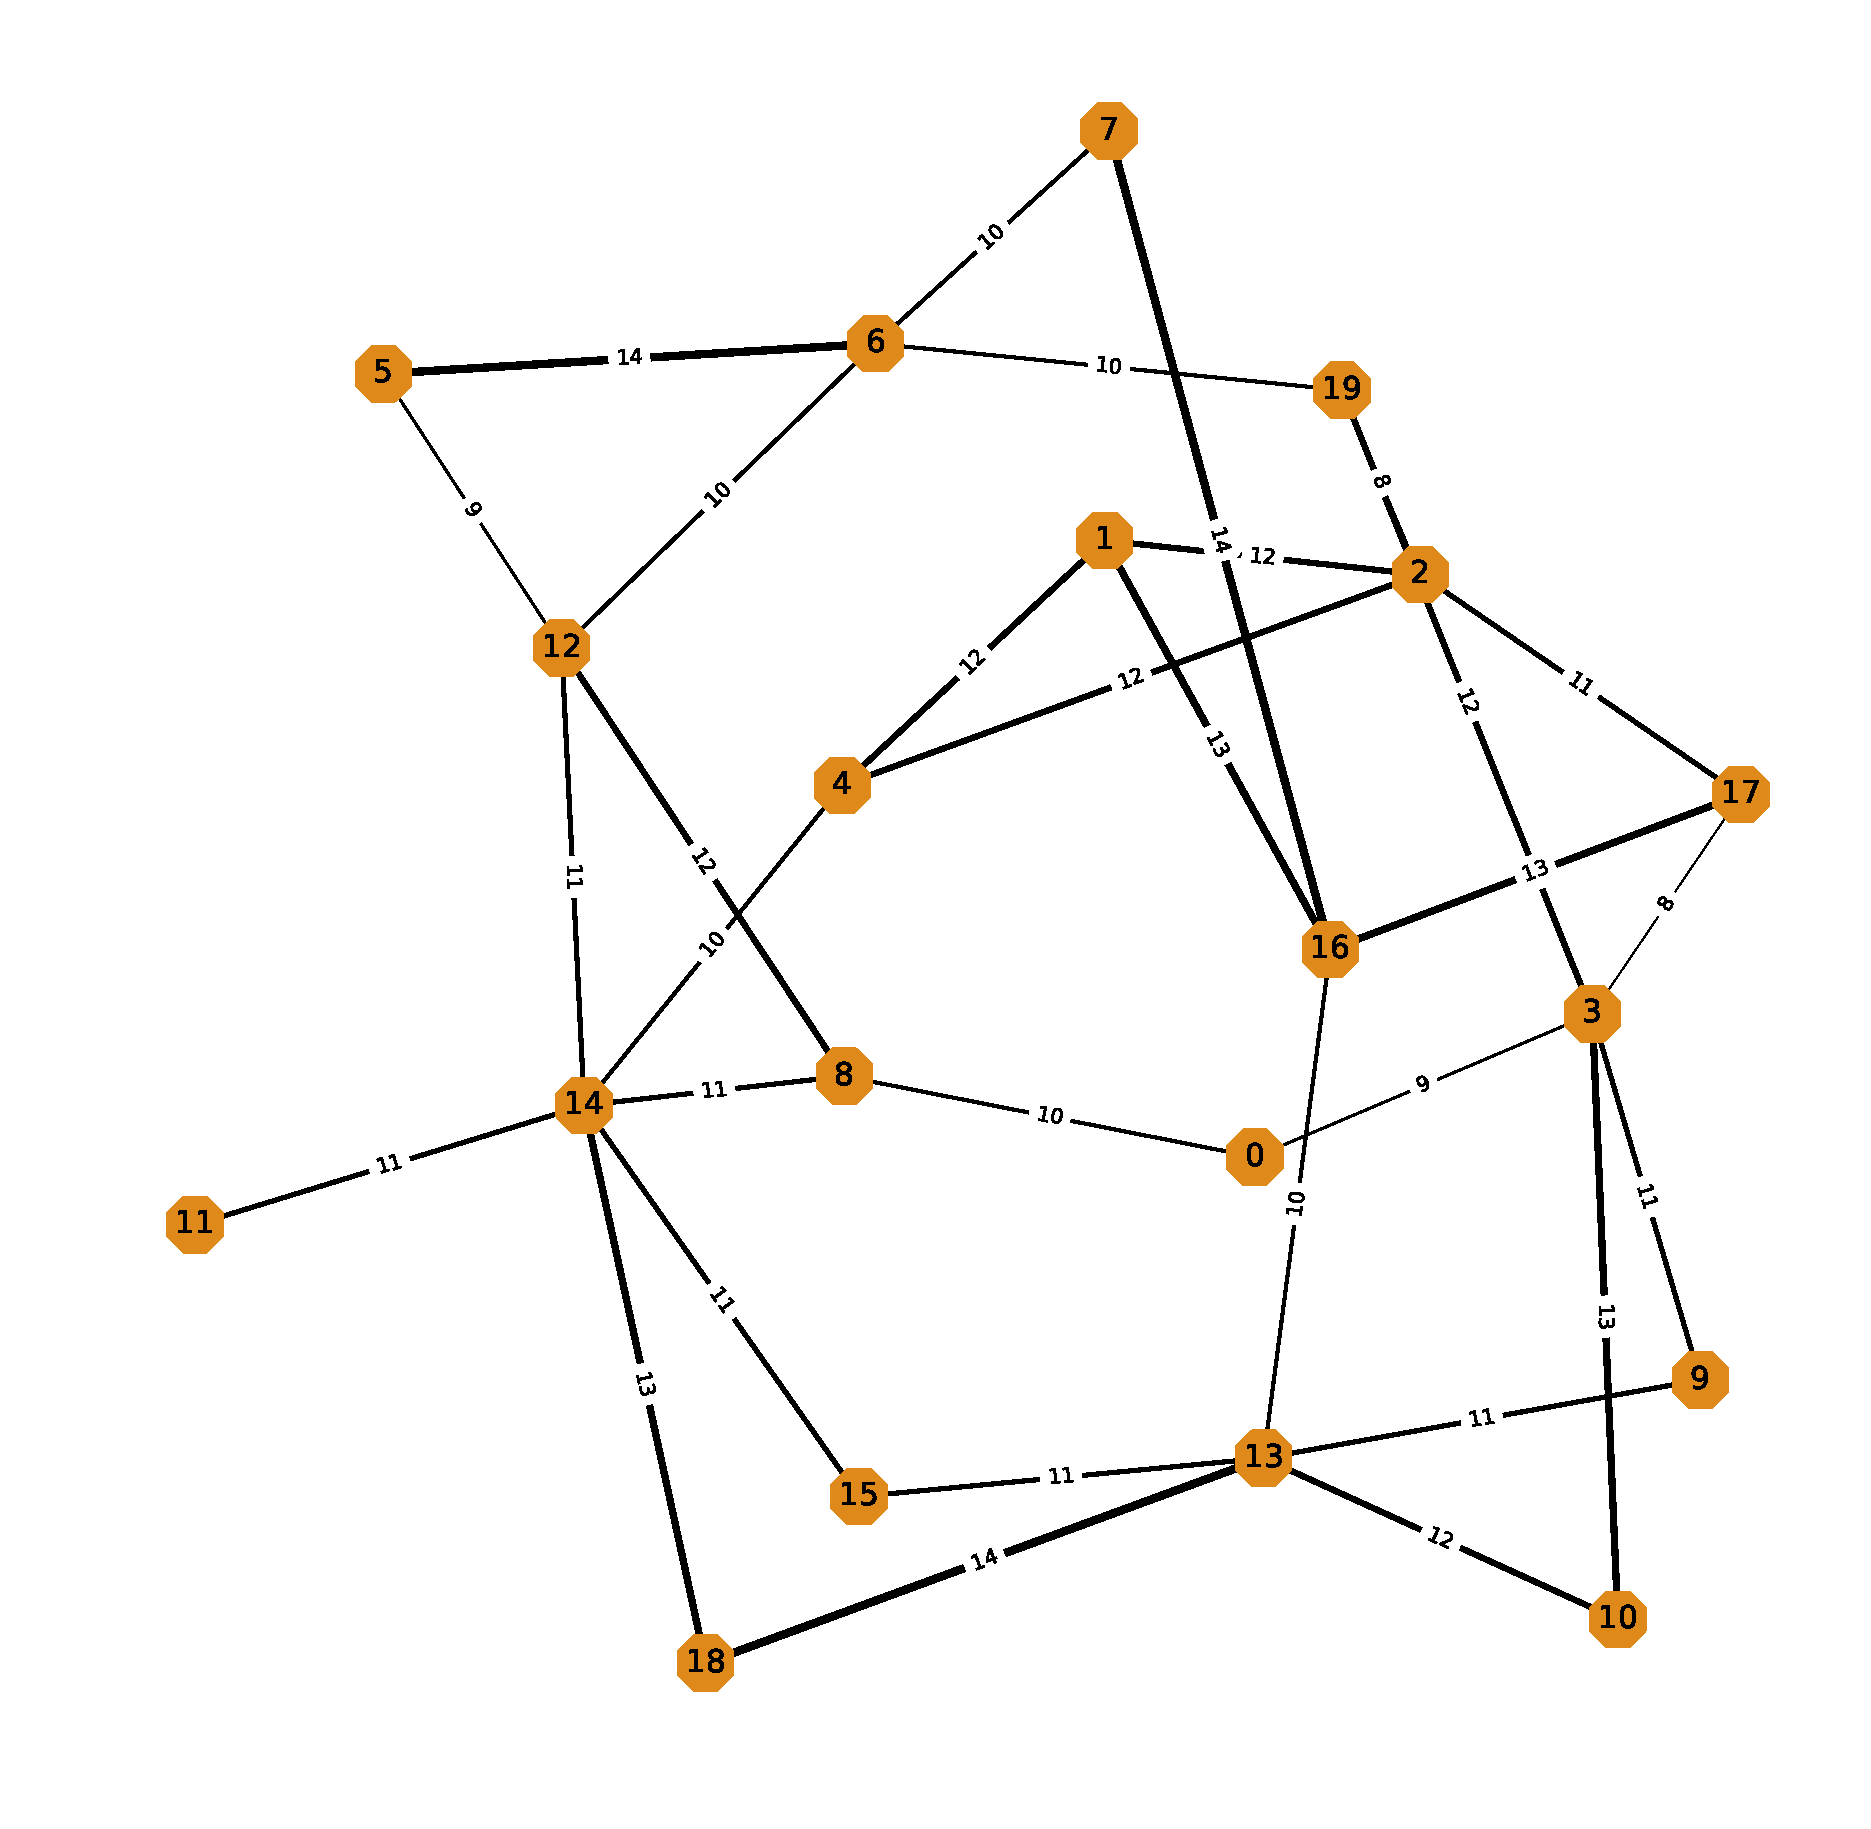
\includegraphics[scale=0.2]{Grafo1a.eps}}
\subfigure[\textit{Grafo2}, con 20 vértices]{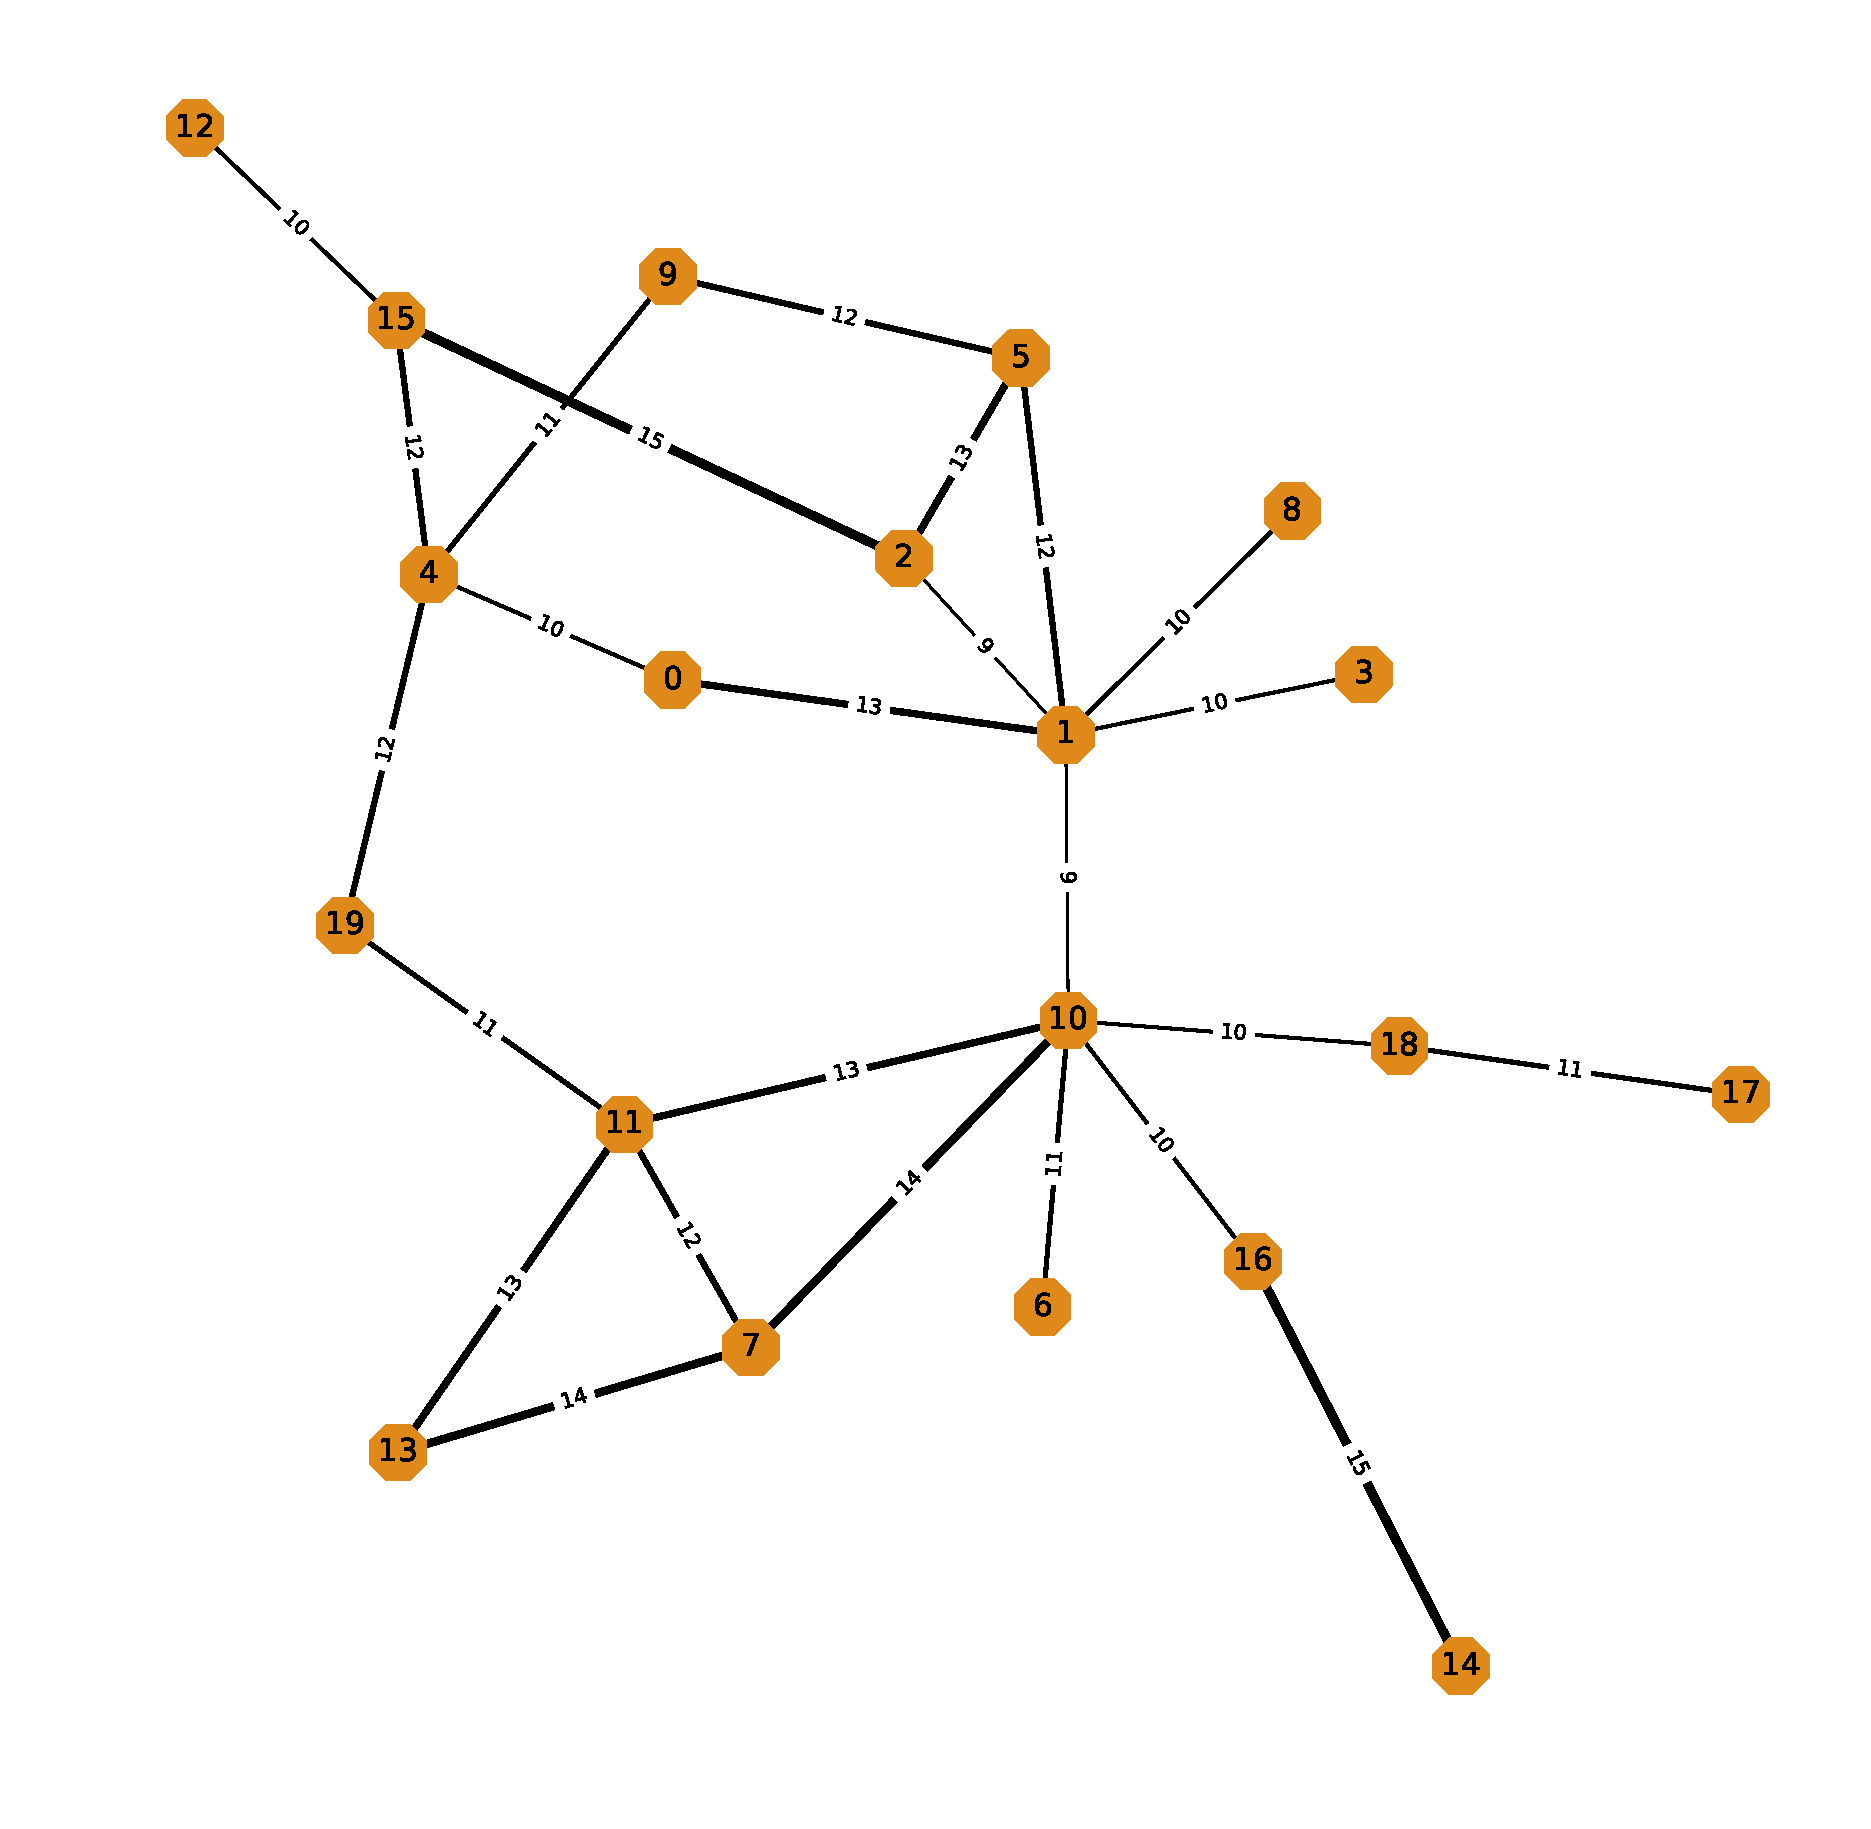
\includegraphics[scale=0.2]{Grafo2a.eps}}
\subfigure[\textit{Grafo3}, con 20 vértices]{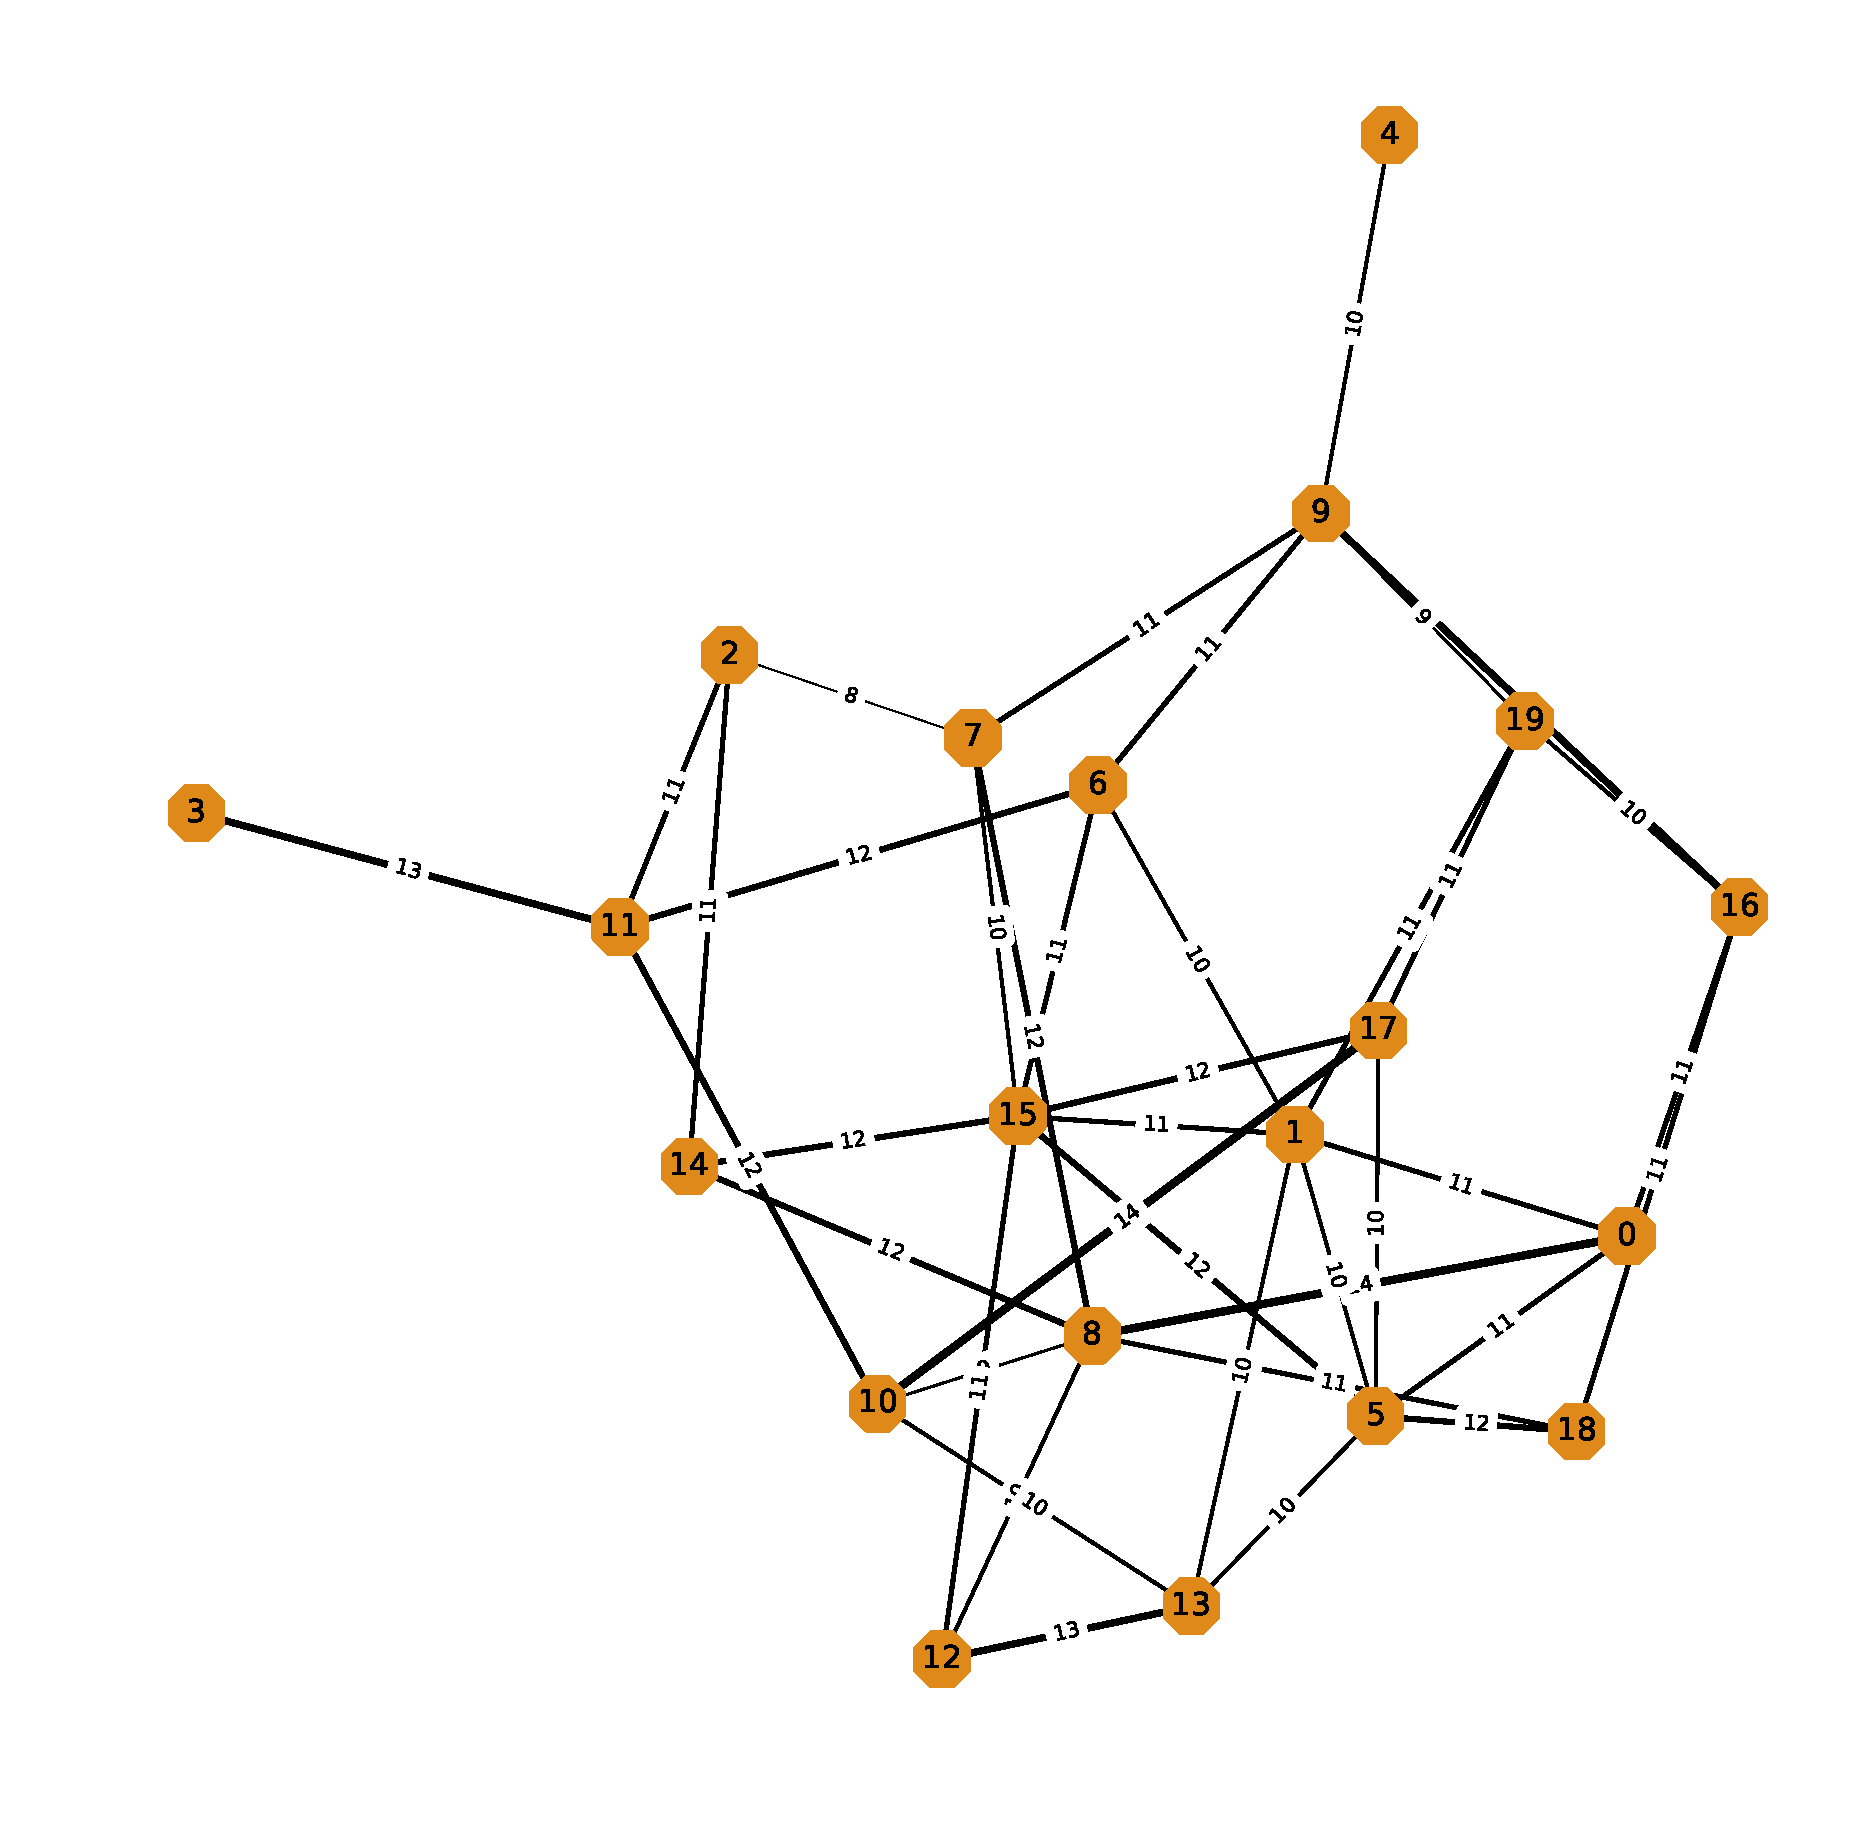
\includegraphics[scale=0.2]{Grafo3a.eps}}
\subfigure[\textit{Grafo4}, con 20 vértices]{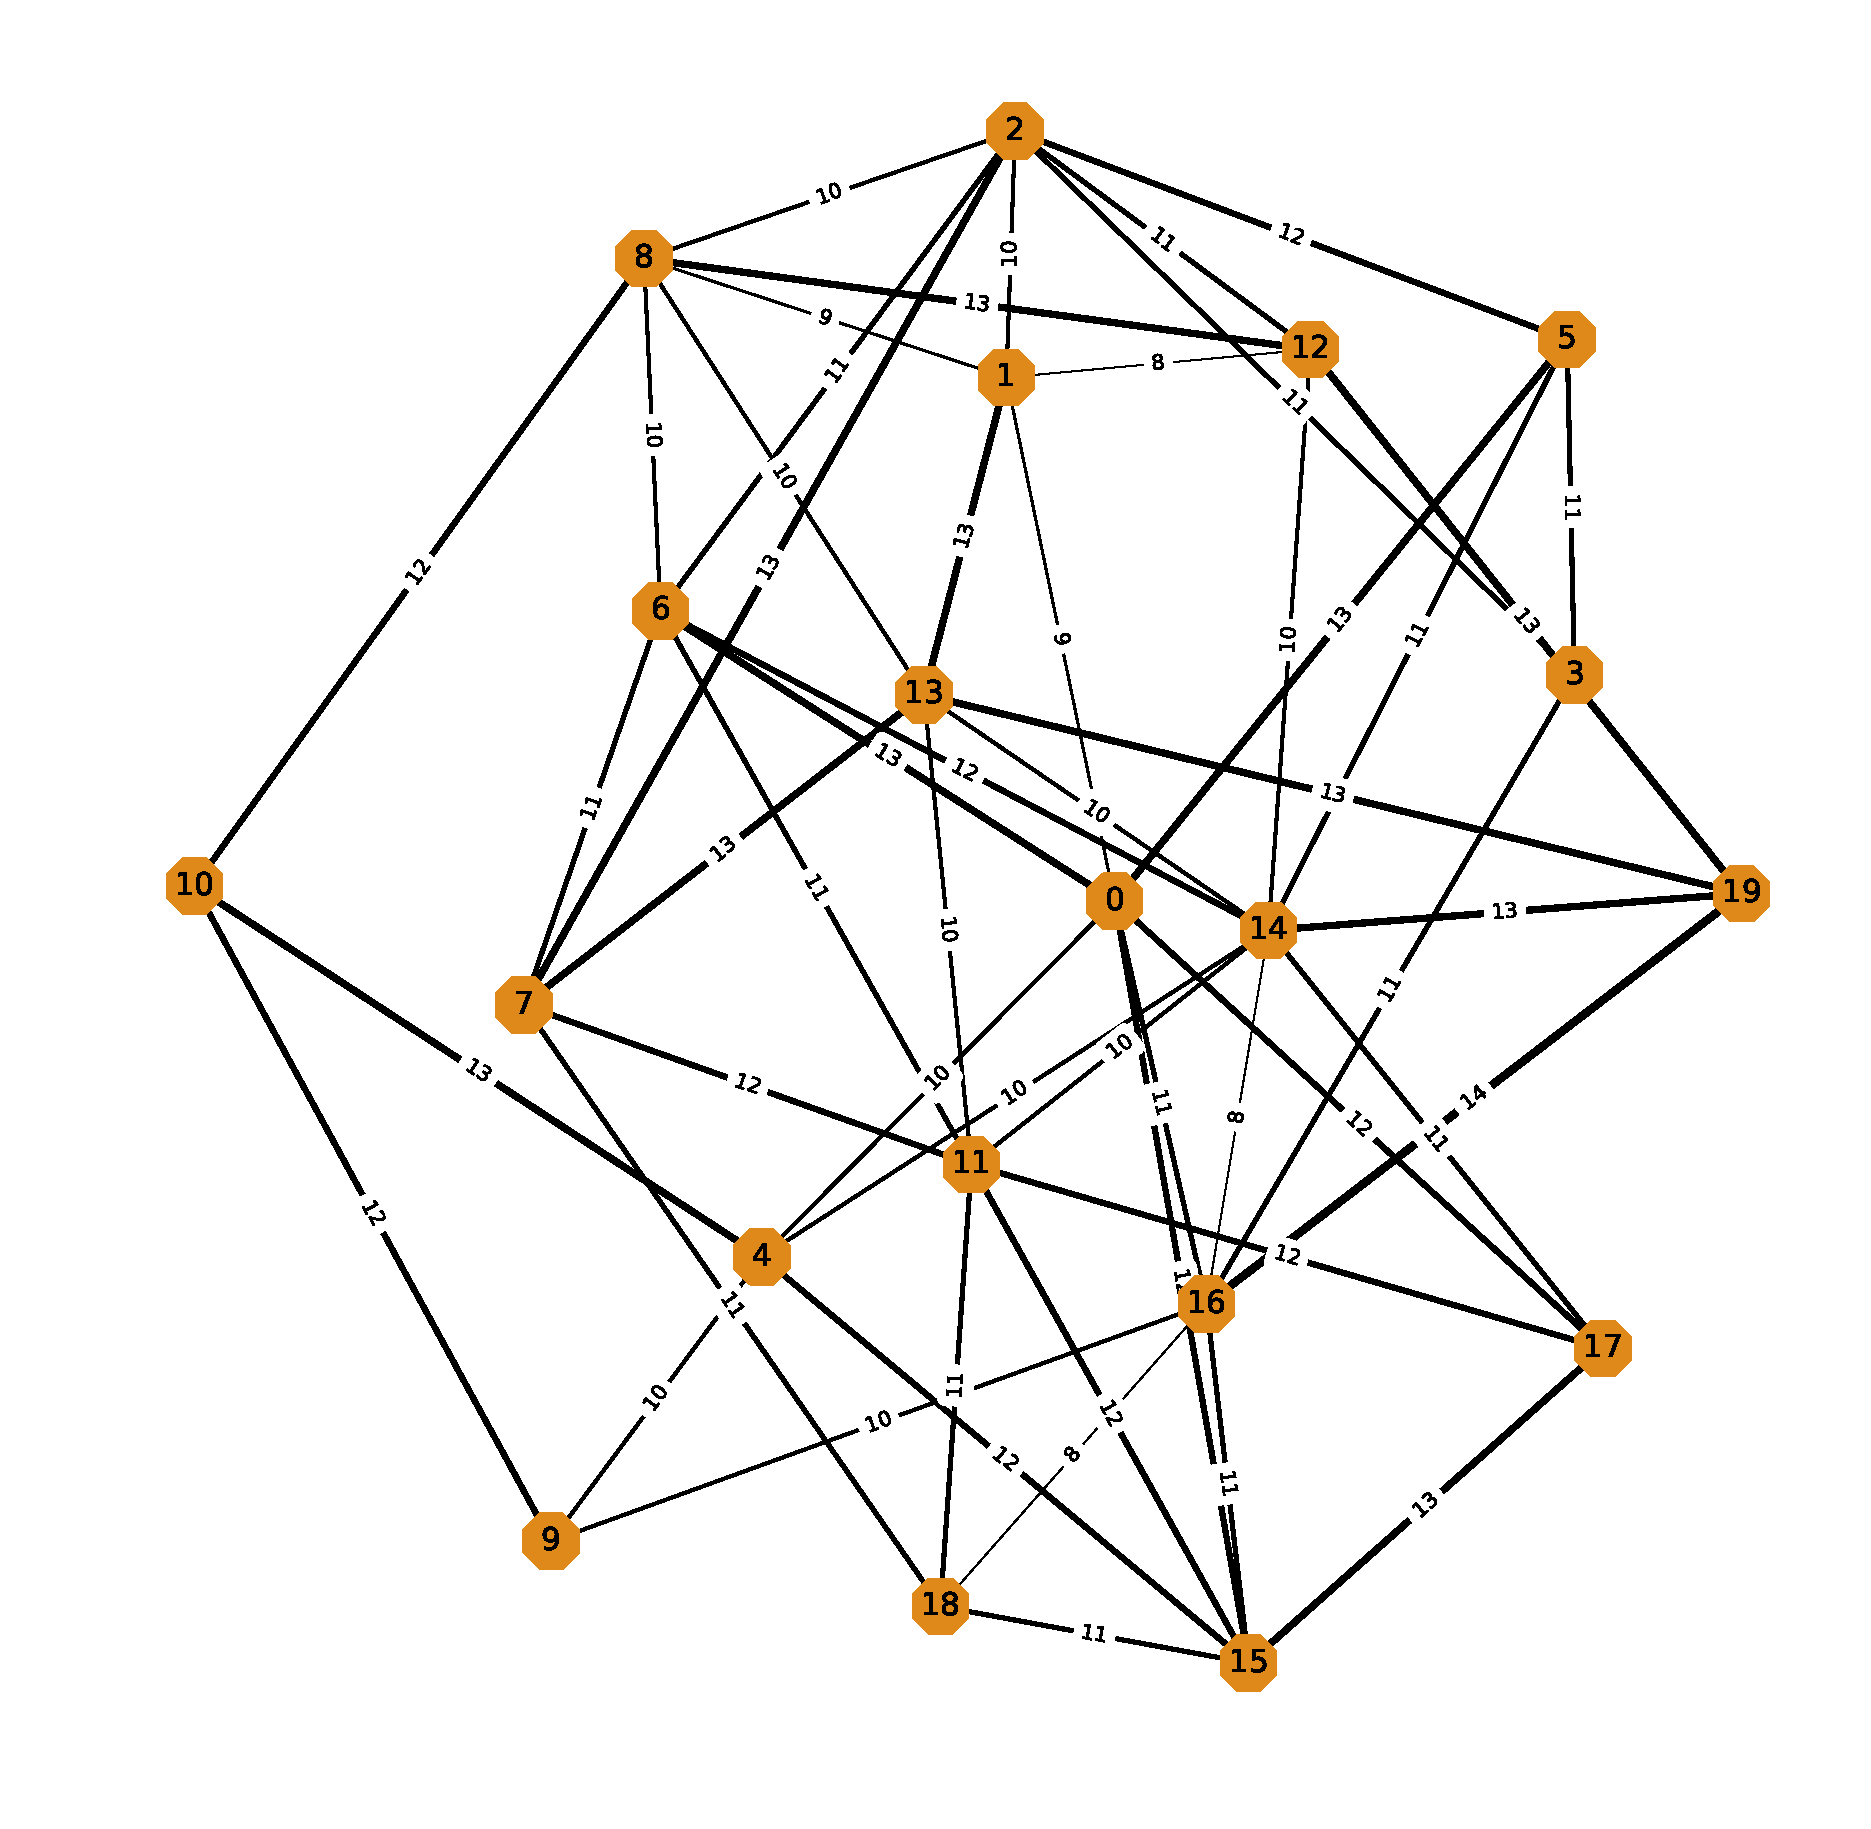
\includegraphics[scale=0.2]{Grafo4a.eps}}
\subfigure[\textit{Grafo5}, con 20 vértices]{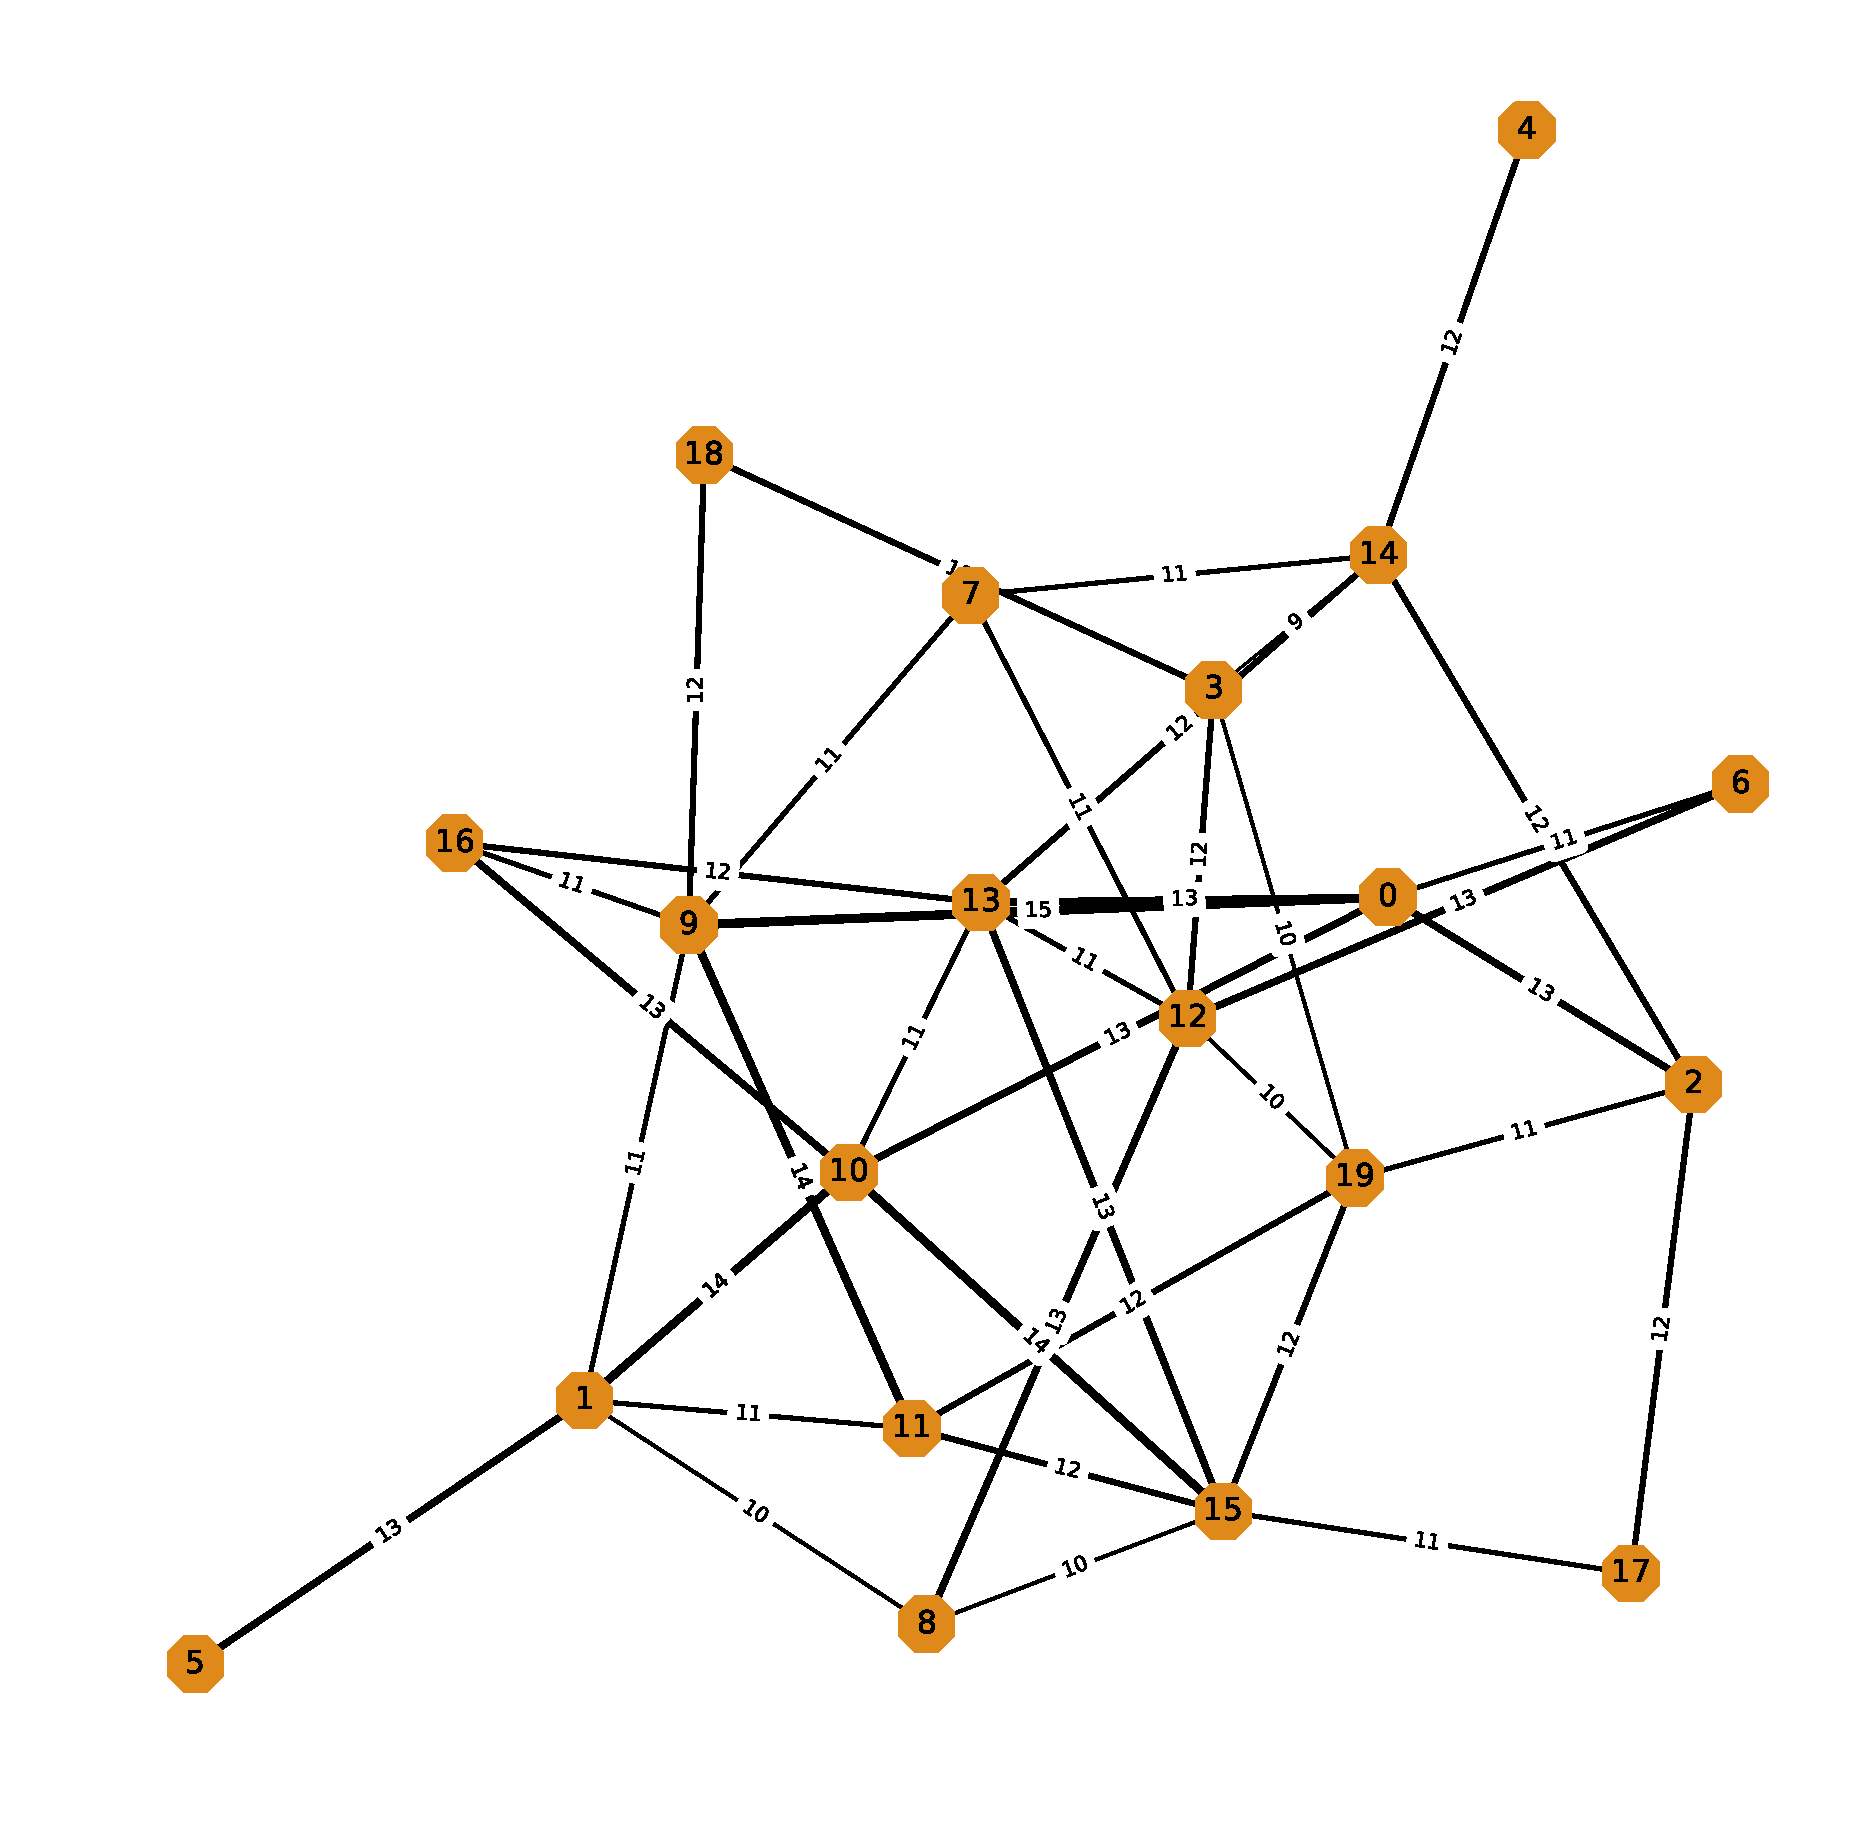
\includegraphics[scale=0.3]{Grafo5a.eps}}
\caption{Grafos generados con el algoritmo seleccionado, donde el grosor de las aristas representan la capacidad de las mismas.}
\label{fig1} 
\end{figure}


\newpage
\section{Algoritmo de flujo máximo.}
En los problemas de flujo en redes, las aristas representan vías por las que puede circular elementos: datos, agua, corriente eléctrica, llamadas telefónicas entre otras. Los pesos de las aristas representan la capacidad máxima de una vía: velocidad de una conexión, volumen máximo de agua, voltaje de una línea eléctrica,cantidad máxima llamadas entre otras; aunque es posible que la cantidad real de flujo sea menor.

El problema del flujo máximo consiste en lo siguiente: dado un grafo con pesos, $G = (V, A, W)$, que representa las capacidades máximas de los canales, un vértice fuente $f$ y otro sumidero $s$ en $ V $, encontrar la cantidad máxima de flujo que puede circular desde $f$ hasta $s$.

En la biblioteca de \textit{networkx} encontramos varios algoritmos con los que podemos atacar los problemas de flujo máximo, para la realización de esta tarea se escogerá uno de los tres algoritmos utilizados en la tarea anterior pertenecientes a dicha librería. Basándonos en los resultados obtenidos en las pruebas realizadas en la tarea anterior.

Los algoritmos escogidos en la tarea anterior son los siguientes:
\begin{itemize}
  \item\textit{Shortest augmenting path} es uno de los enfoques más clásicos para la máxima coincidencia y los problemas de flujo máximo. Sorprendentemente, aunque esta idea es una de las técnicas más básicas, está lejos de ser completamente entendida. Es más fácil hablar de ello introduciendo el problema de emparejamiento bipartito en línea \cite{Bosek2018}. Este algoritmo encuentra el flujo máximo de un solo producto utilizando la ruta de aumento más corto y devuelve la red residual resultante después de calcular el flujo máximo.   
   \item\textit{Maximum flow} encuentra la ruta por la cual pasa la máxima cantidad de flujo, recibe como parámetros un grafo $G$, una fuente $f$, un sumidero $s$ y además una capacidad que de no tenerla, se considera que el borde tiene una capacidad infinita. Se puede aplicar en grafos tanto dirigidos como no dirigidos.) \cite{mf}.
	\item\textit{Preflow push} encuentra un flujo máximo de un solo producto utilizando el algoritmo de empuje previo al flujo de la etiqueta más alta. Esta función devuelve la red residual resultante después de calcular el flujo máximo. Este algoritmo tiene un tiempo de ejecución de $ O(n^{2}\sqrt{m})$ para $n$ vértices y $m$ aristas. \cite{gc}.
\end{itemize}

De los algoritmos anteriores el que se utilisa en esta tarea es el \textit{Shortest augmenting path} por ser el algoritmo que mejores tiempos registró en la tarea anterior.
\section{Algoritmo de acomodo}

El algoritmo \texttt{ Kamada kawai layout} posiciona los nodos utilizando la función de costo de longitud de camino \textit{Kamada-Kawai}, dando la mejor visualización de los grafos generados.

\section{Generación de datos}
Con el objetivo de realizar las mediciones de los tiempos de ejecución de los algoritmo de flujo máximo seleccionado asi como el calculo de las seis propiedades de los nodos (distribución de grado, coeficiente de agrupamiento, centralidad de cercanía, centralidad de carga, excentricidad,\textit{pagerank}) se desarrolló el siguiente código.

En primer lugar, se crea una función (\texttt{Maxflow()}) que recibe como parámetros el grafo al que se le aplicara el algoritmo (\texttt{G}), la fuente (\texttt{a}) y sumidero (\texttt{b}). Al llamar esta función se genera con cada ejecución los datos que son guardados en un \textit{data frame} del cual se muestra un fragmento en el cuadro \ref{tab:tab1} de la página \pageref{tab:tab1}.
% Table generated by Excel2LaTeX from sheet 'Hoja1'
\begin{table}[htbp]
  \centering
  
  \caption{Fragmento del \textit{data frame} que contiene los datos recopilados.}
  \resizebox{\textwidth}{!}{
    \begin{tabular}{cccccccccccc}
    \toprule
    \textbf{Grafo} & \textbf{Fuente} & \textbf{Sumidero} & \textbf{Media} & \textbf{Mediana} & \textbf{FlujoMax} & \textbf{Grado} & \textbf{CoefAg} & \textbf{CentCer} & \textbf{CentCag} & \textbf{Excent} & \textbf{PageRag} \\
    \midrule
    Grafo1 & 0     & 1     & 0.026 & 0.020 & 19    & 2     & 0.000 & 0.388 & 0.048 & 4     & 0.035 \\
    Grafo1 & 15    & 7     & 0.022 & 0.020 & 22    & 2     & 0.000 & 0.413 & 0.035 & 4     & 0.034 \\
    Grafo2 & 0     & 9     & 0.029 & 0.020 & 23    & 2     & 0.000 & 0.396 & 0.044 & 4     & 0.039 \\
    Grafo2 & 2     & 4     & 0.028 & 0.024 & 34    & 3     & 0.333 & 0.404 & 0.123 & 4     & 0.056 \\
    Grafo3 & 1     & 2     & 0.044 & 0.052 & 30    & 6     & 0.267 & 0.543 & 0.084 & 3     & 0.068 \\
    Grafo3 & 1     & 15    & 0.042 & 0.024 & 63    & 6     & 0.267 & 0.543 & 0.084 & 3     & 0.068 \\
    Grafo4 & 0     & 13    & 0.079 & 0.084 & 69    & 7     & 0.143 & 0.613 & 0.096 & 2     & 0.064 \\
    Grafo4 & 3     & 10    & 0.055 & 0.032 & 33    & 3     & 0.333 & 0.475 & 0.016 & 3     & 0.032 \\
    Grafo5 & 3     & 15    & 0.020 & 0.020 & 43    & 4     & 0.167 & 0.463 & 0.059 & 4     & 0.052 \\
    Grafo5 & 8     & 2     & 0.076 & 0.074 & 33    & 3     & 0.000 & 0.452 & 0.034 & 4     & 0.039 \\
    \bottomrule
    \end{tabular}%
    }
  \label{tab:tab1}%
\end{table}%

En este fragmento del código se realiza toda la recopilación de la información necesaria para el análisis de los factores que in fluyen en el tiempo de ejecución y el flujo máximo, también dibuja los grafos a los que se les aplico el algoritmo. 
\begin{center}
\lstinputlisting[language=Python, firstline=14, lastline=154]{Leer_grafo.py}
\end{center}
La aplicación del algoritmo de flujo máximo \textit{Shortest augmenting path} a todas las posibles combinaciones de fuentes y sumidero de cada uno de los cinco grafos nos dio como resultado los valores de flujo máximo para cada una de estas combinaciones y nos muestra cómo va variando el óptimo desde la peor combinación fuente sumidero a la mejor.

Para el Grafo1 esto se muestra en la figura \ref{fig2} de la página \pageref{fig2}.

\begin{figure}[htbp]

\subfigure[\textit{Grafo1}, flujo máximo 11]{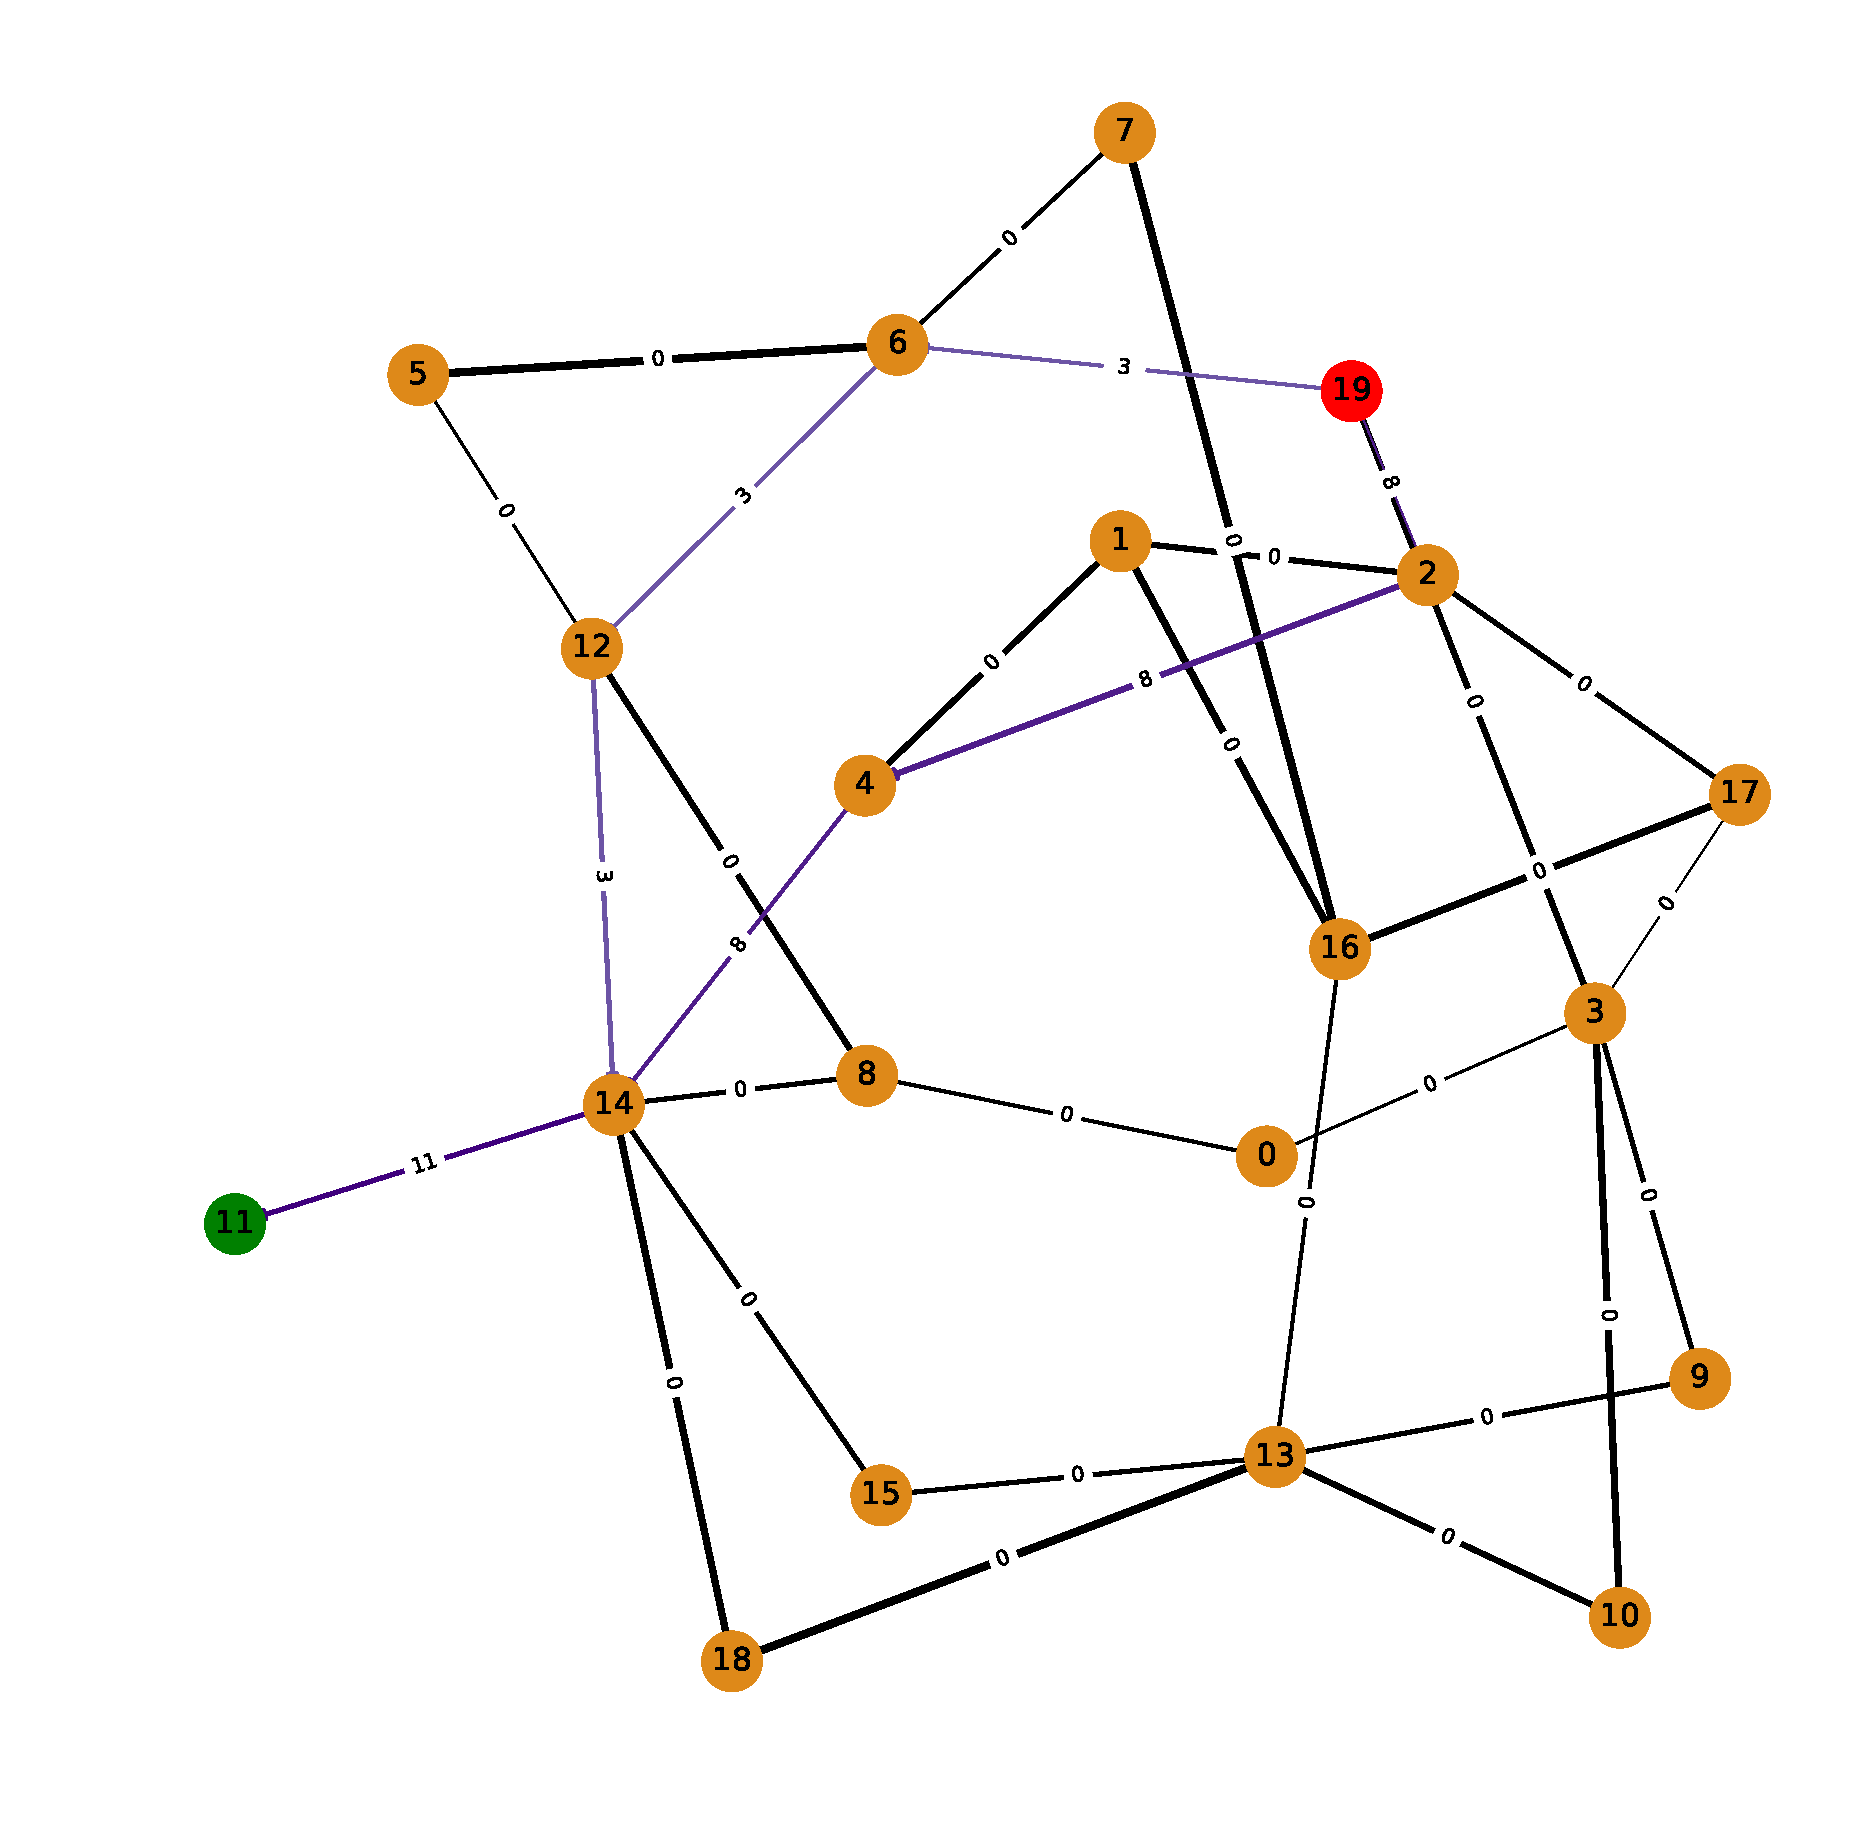
\includegraphics[scale=0.22]{Grafo1mf.eps}}
\subfigure[\textit{Grafo1}, flujo máximo 32]{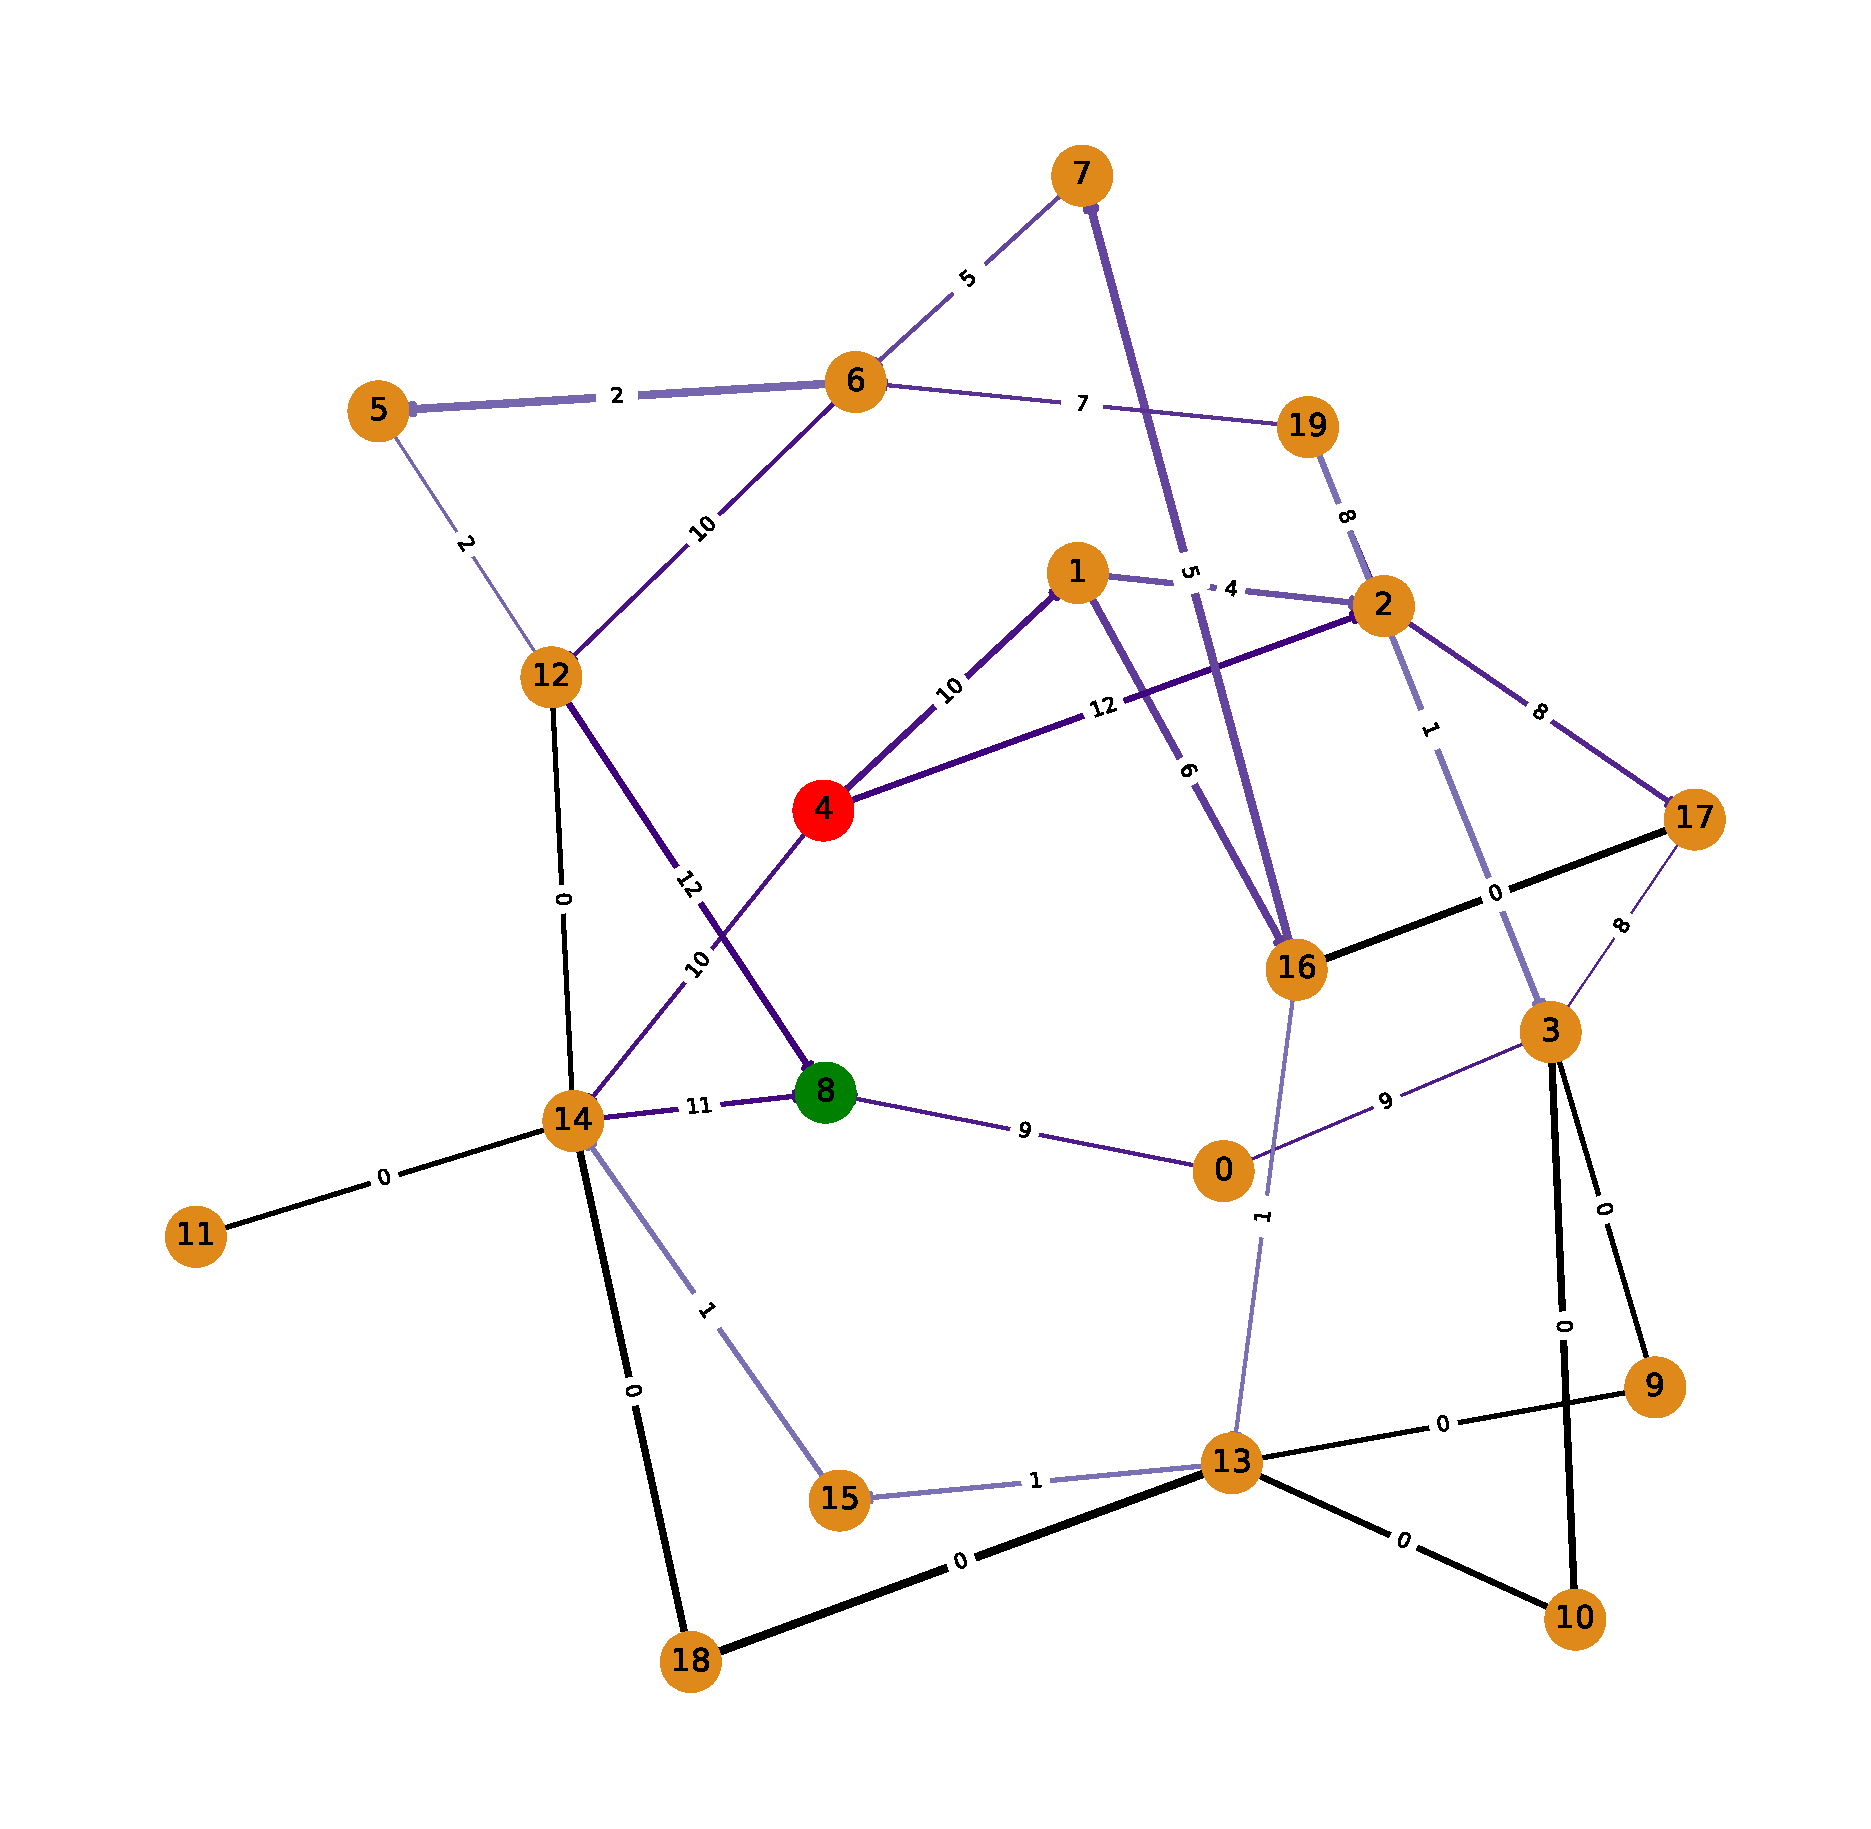
\includegraphics[scale=0.22]{Grafo1cf.eps}}
\subfigure[\textit{Grafo1}, flujo máximo 52]{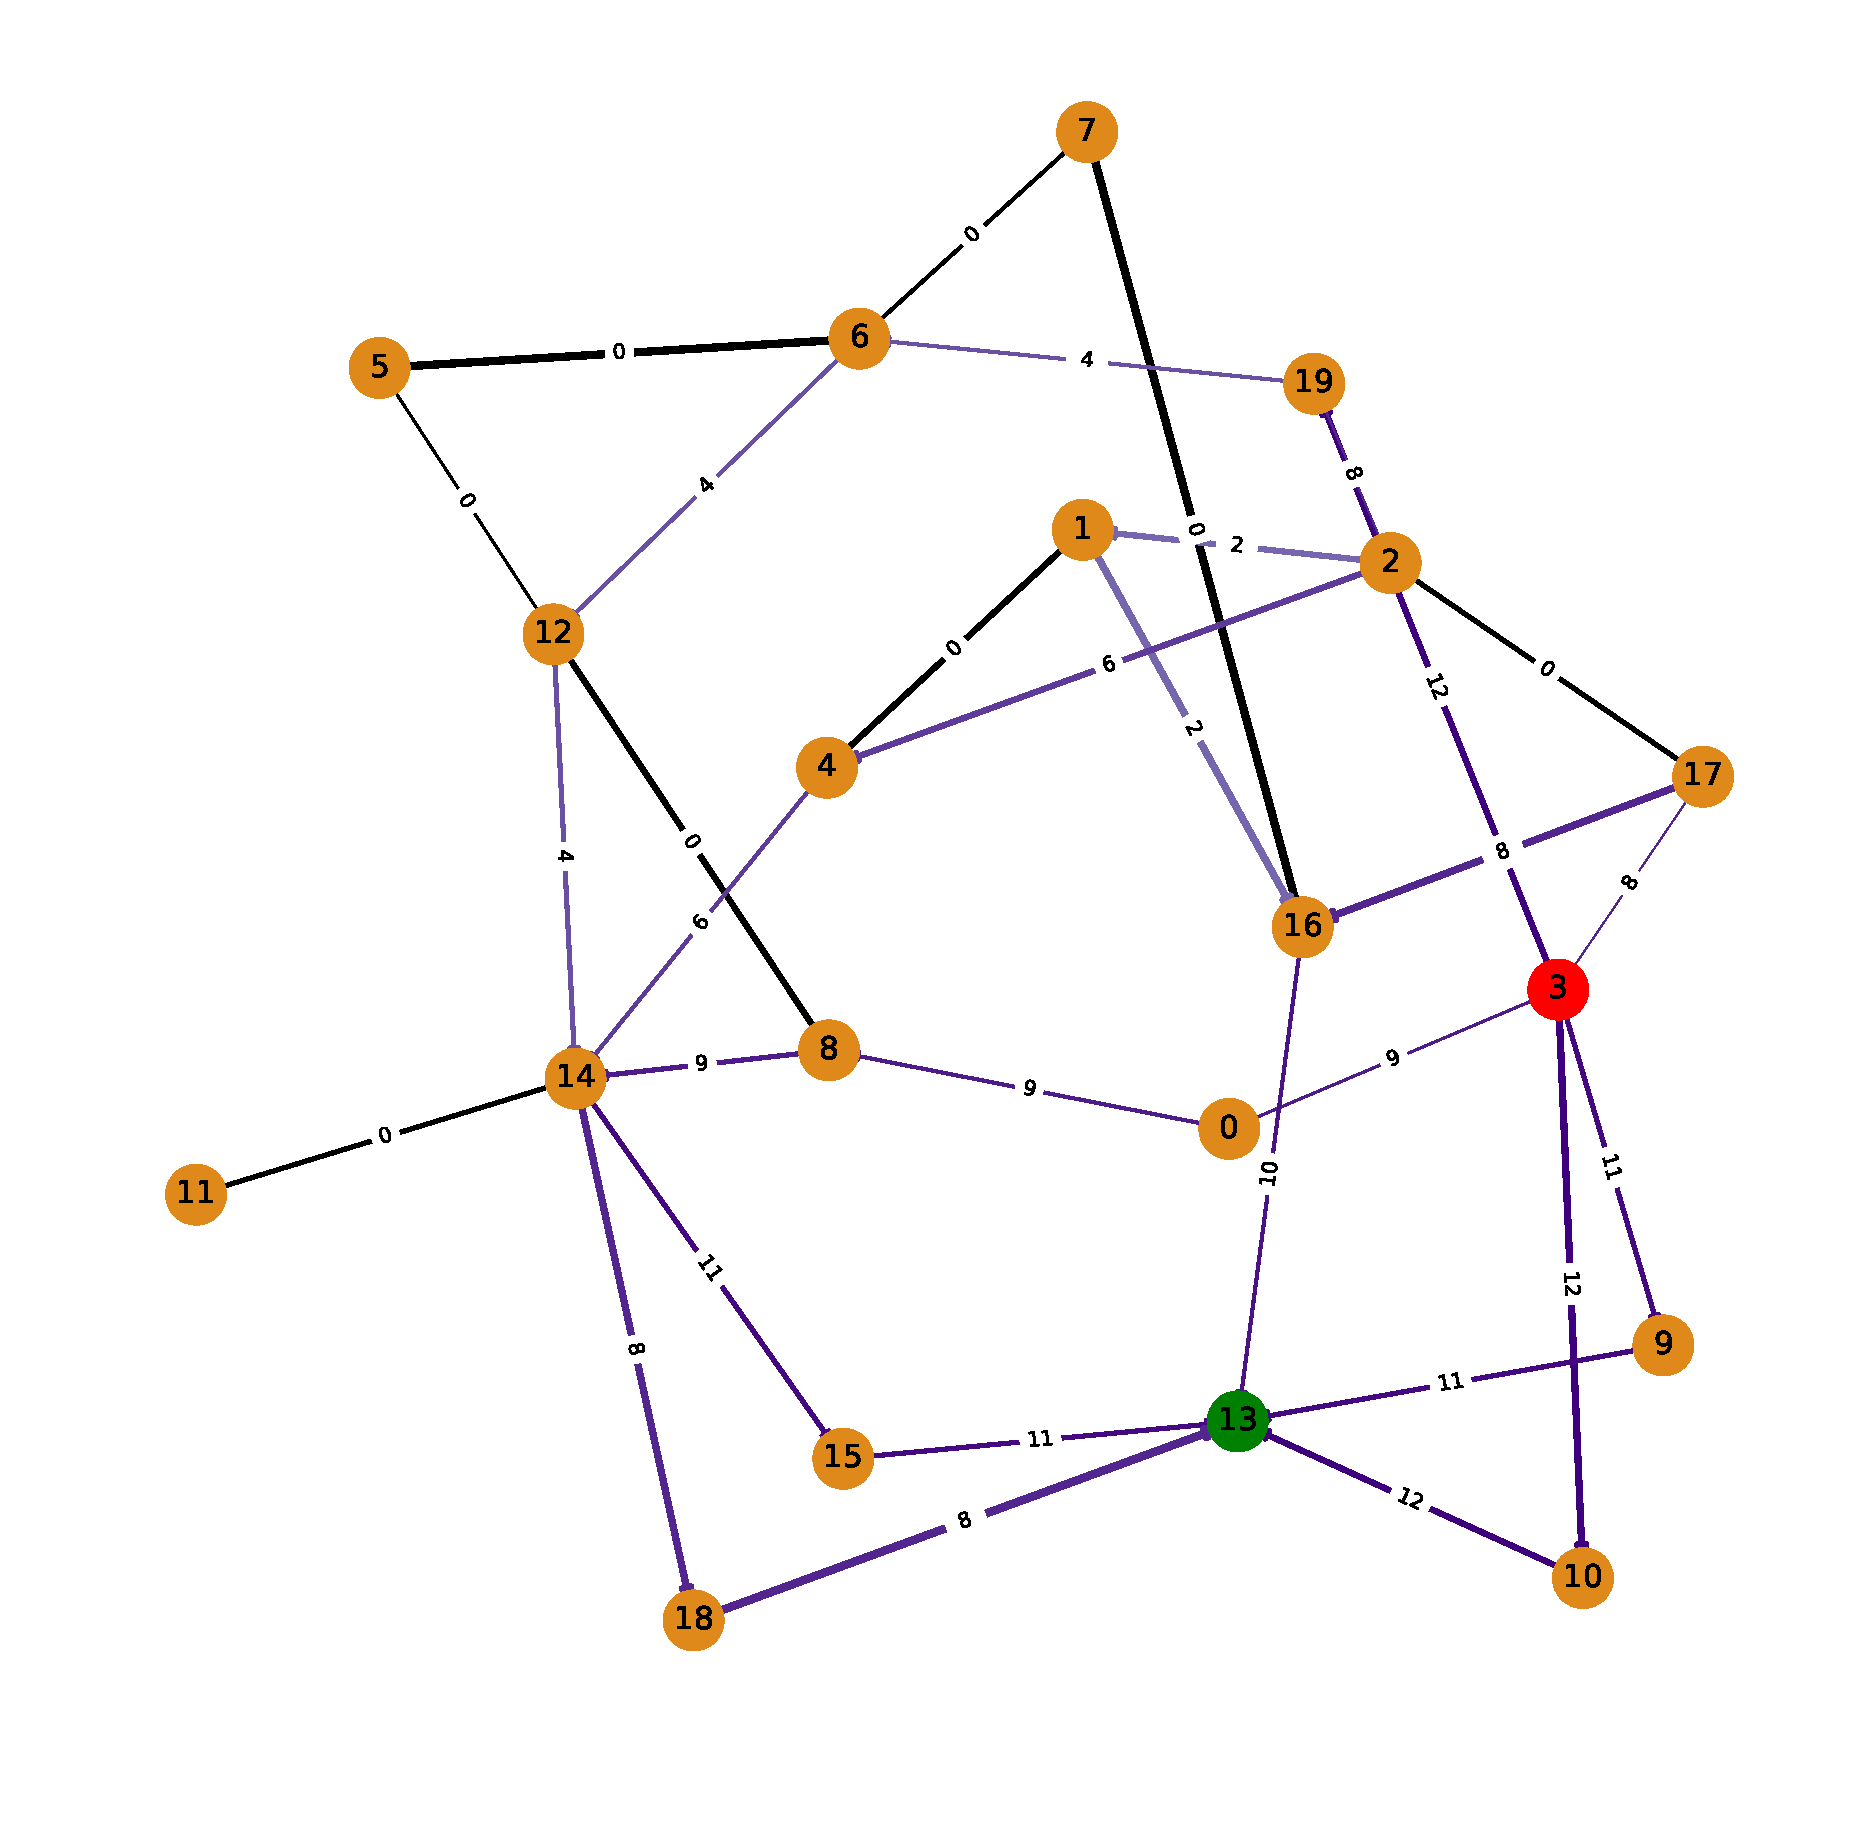
\includegraphics[scale=0.22]{Grafo1bf.eps}}
\subfigure[\textit{Grafo1}, flujo máximo 56]{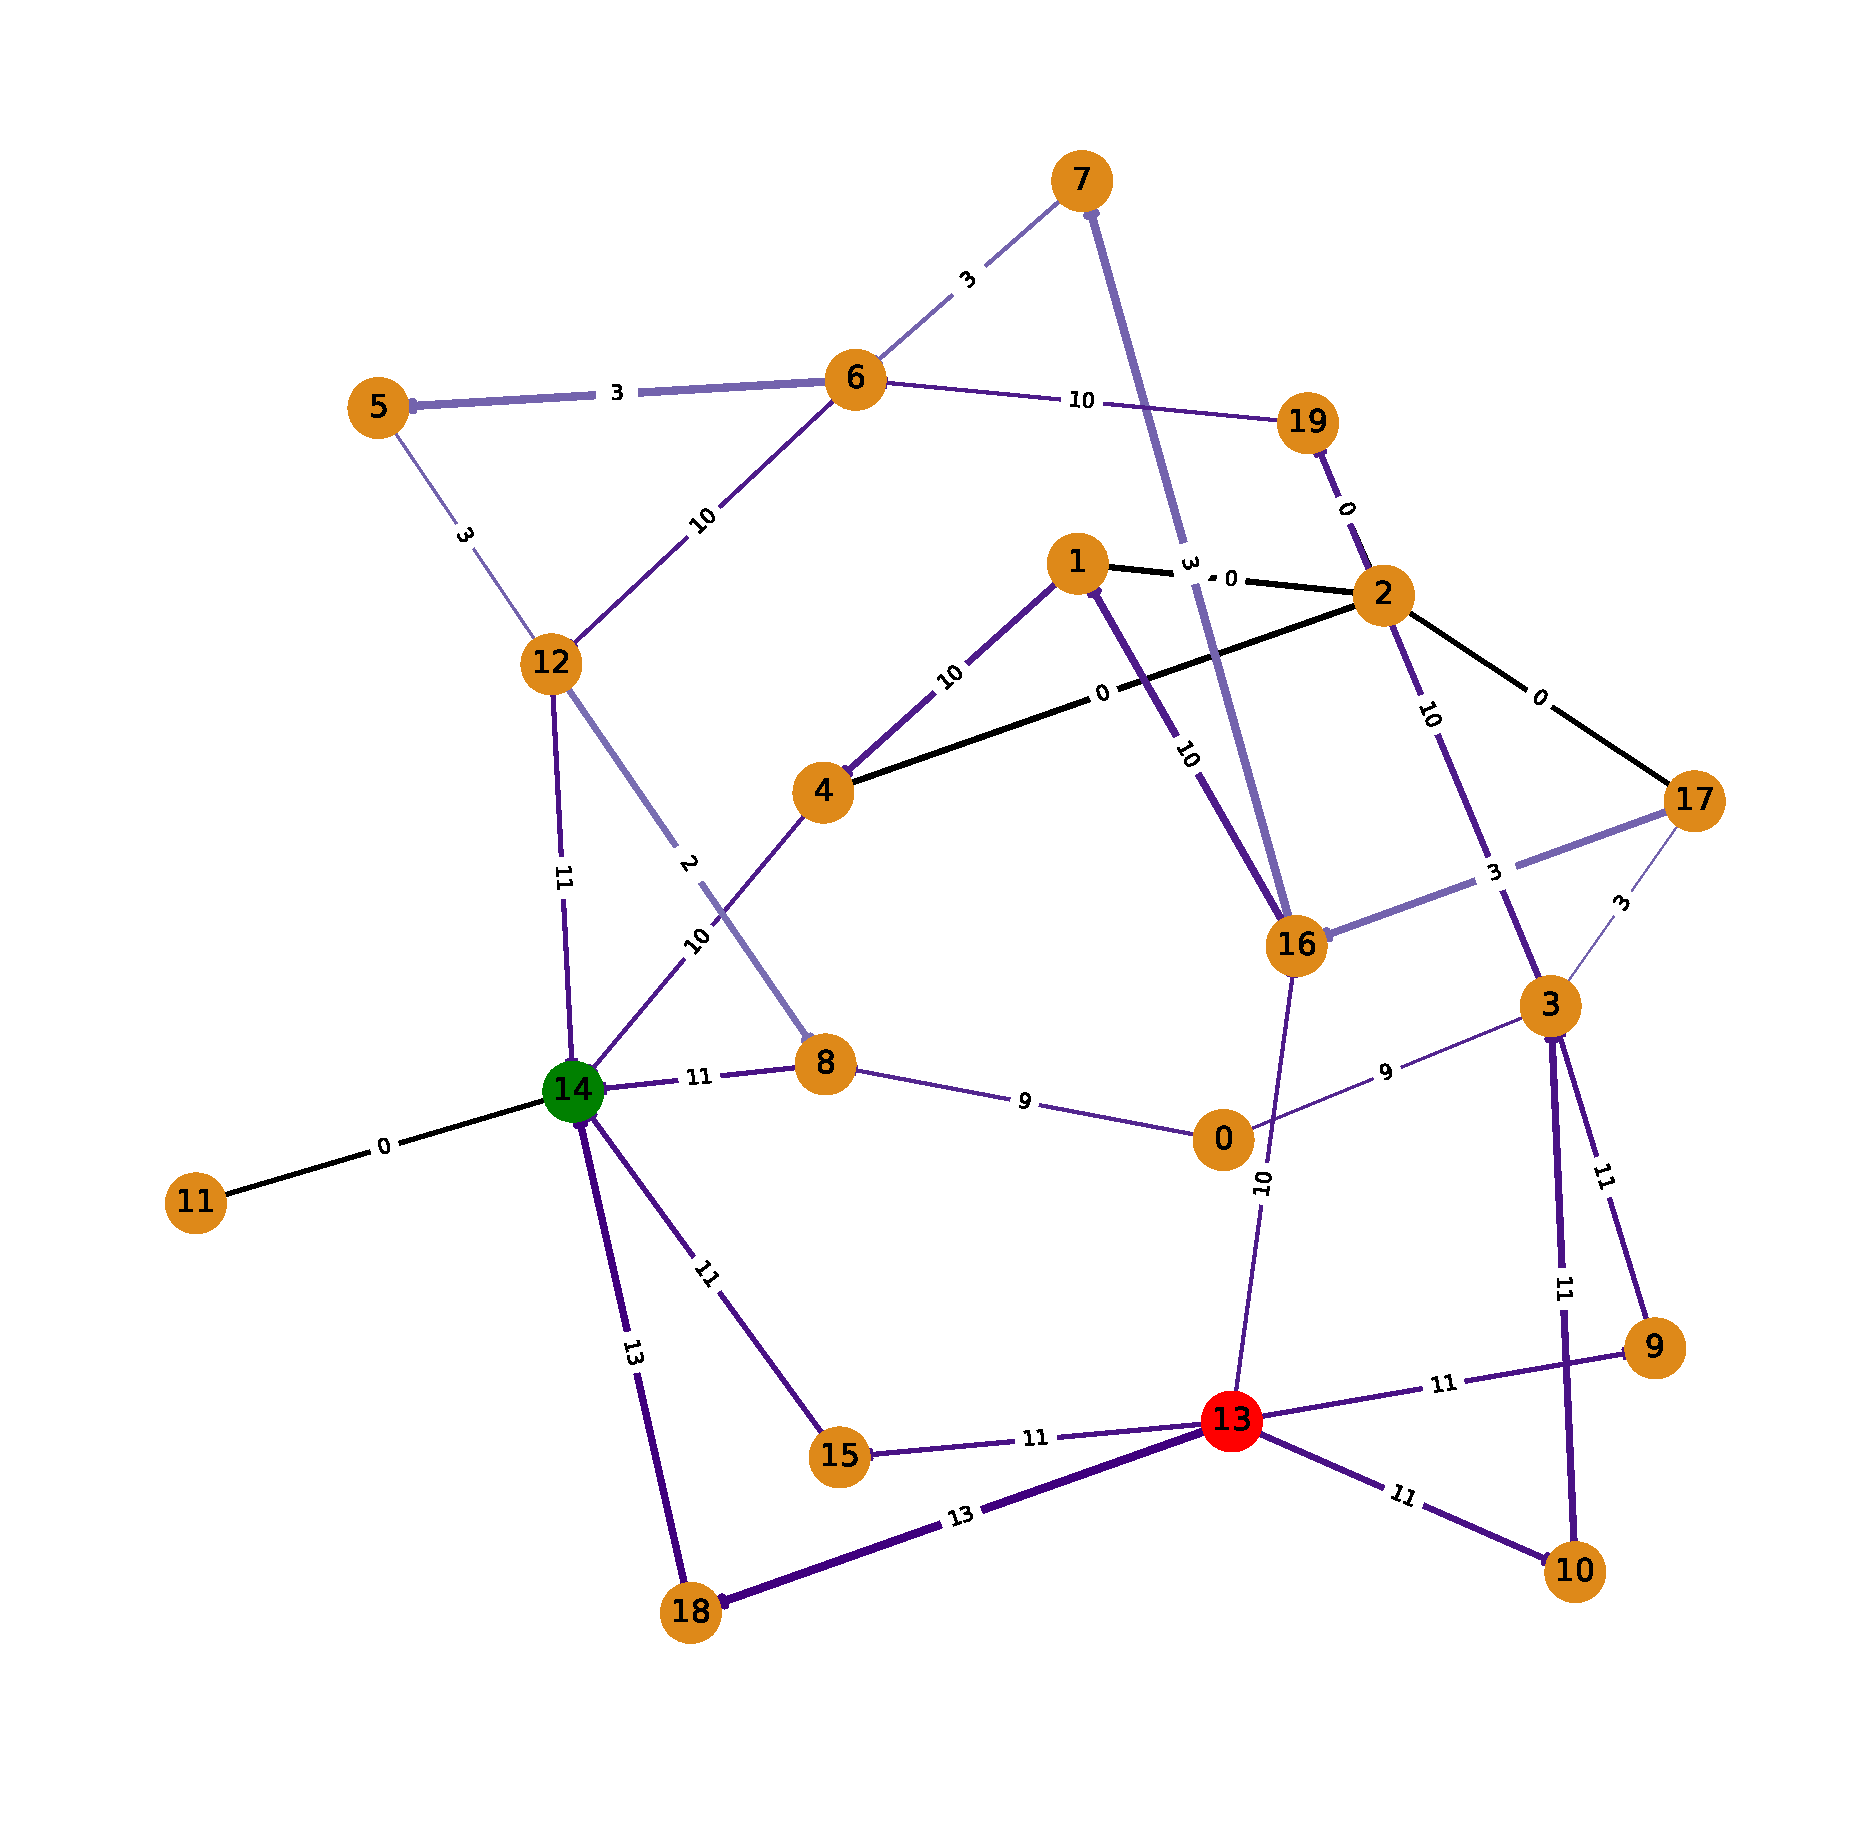
\includegraphics[scale=0.32]{Grafo1af.eps}}

\caption{Grafos resultantes de la aplicación del algoritmo de flujo máximo, donde el grosor de las aristas representa la capacidad de las mismas, el color negro la ausencia de flujo, el color violeta la presencia de flujo y la intensidad del color violeta la cantidad de flujo que pasa por la arista. El color rojo del vértice representa la fuente y el vértice verde el sumidero. }
\label{fig2} 
\end{figure}

Para el Grafo2 esto se muestra en la figura \ref{fig3} de la página \pageref{fig3}.

\begin{figure}[htbp]

\subfigure[\textit{Grafo2}, flujo máximo 10]{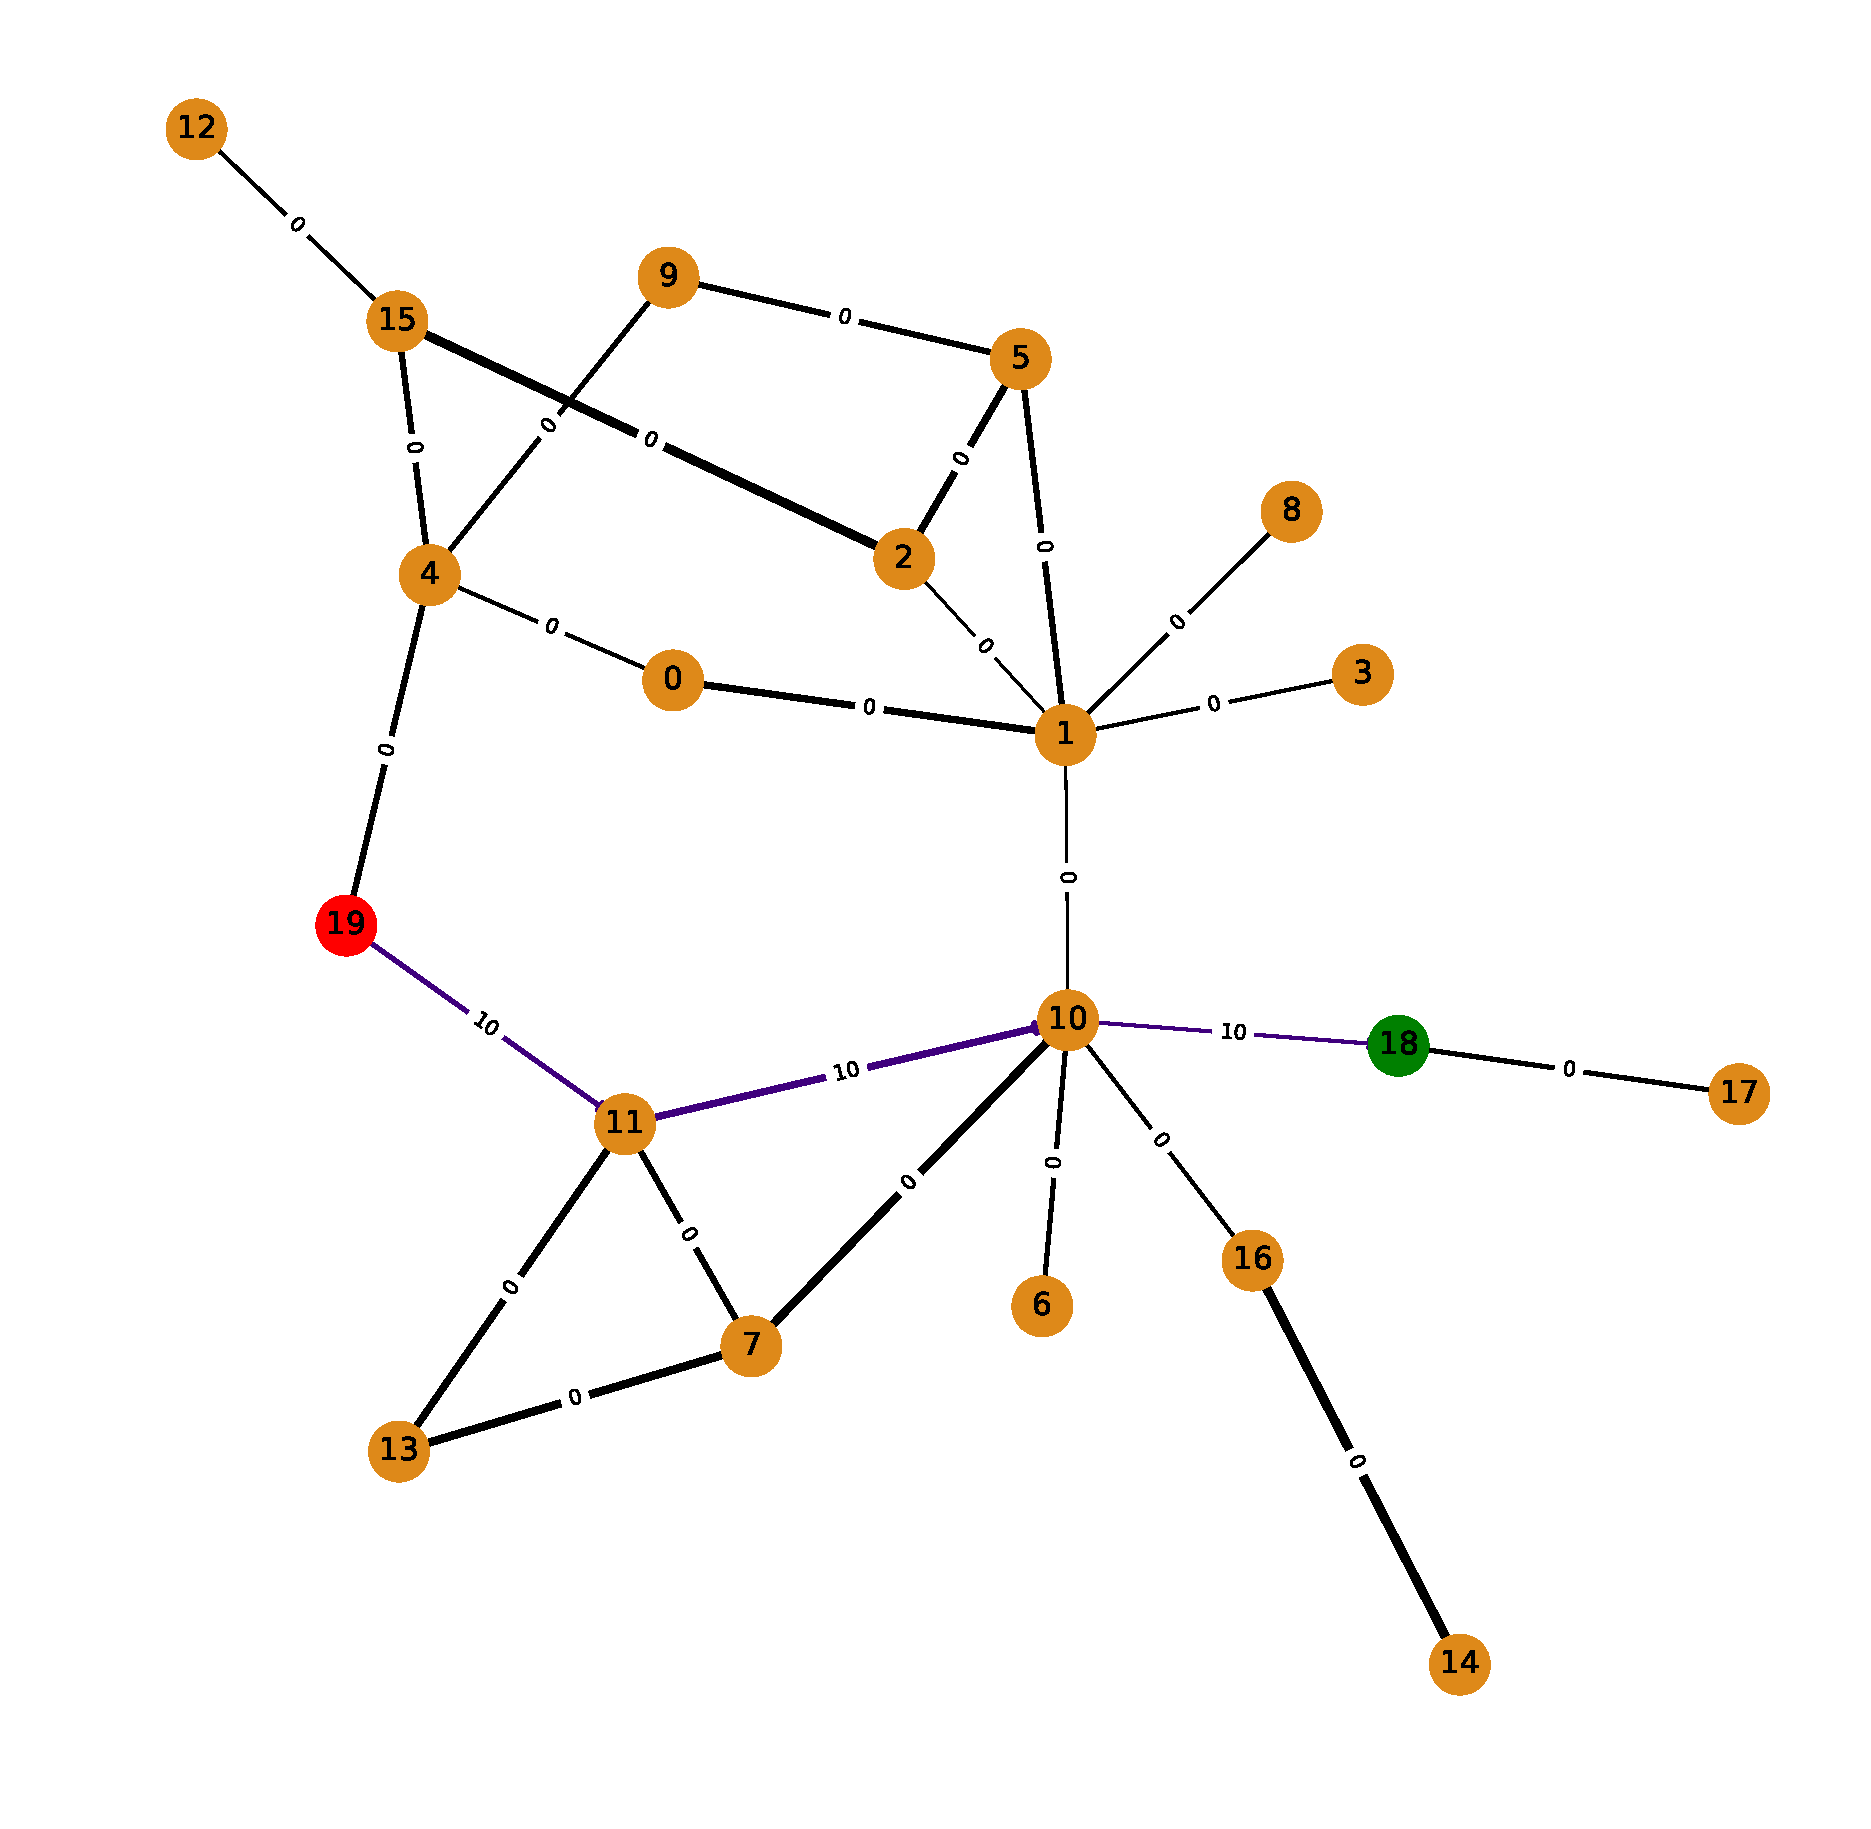
\includegraphics[scale=0.22]{Grafo2mf.eps}}
\subfigure[\textit{Grafo2}, flujo máximo 36]{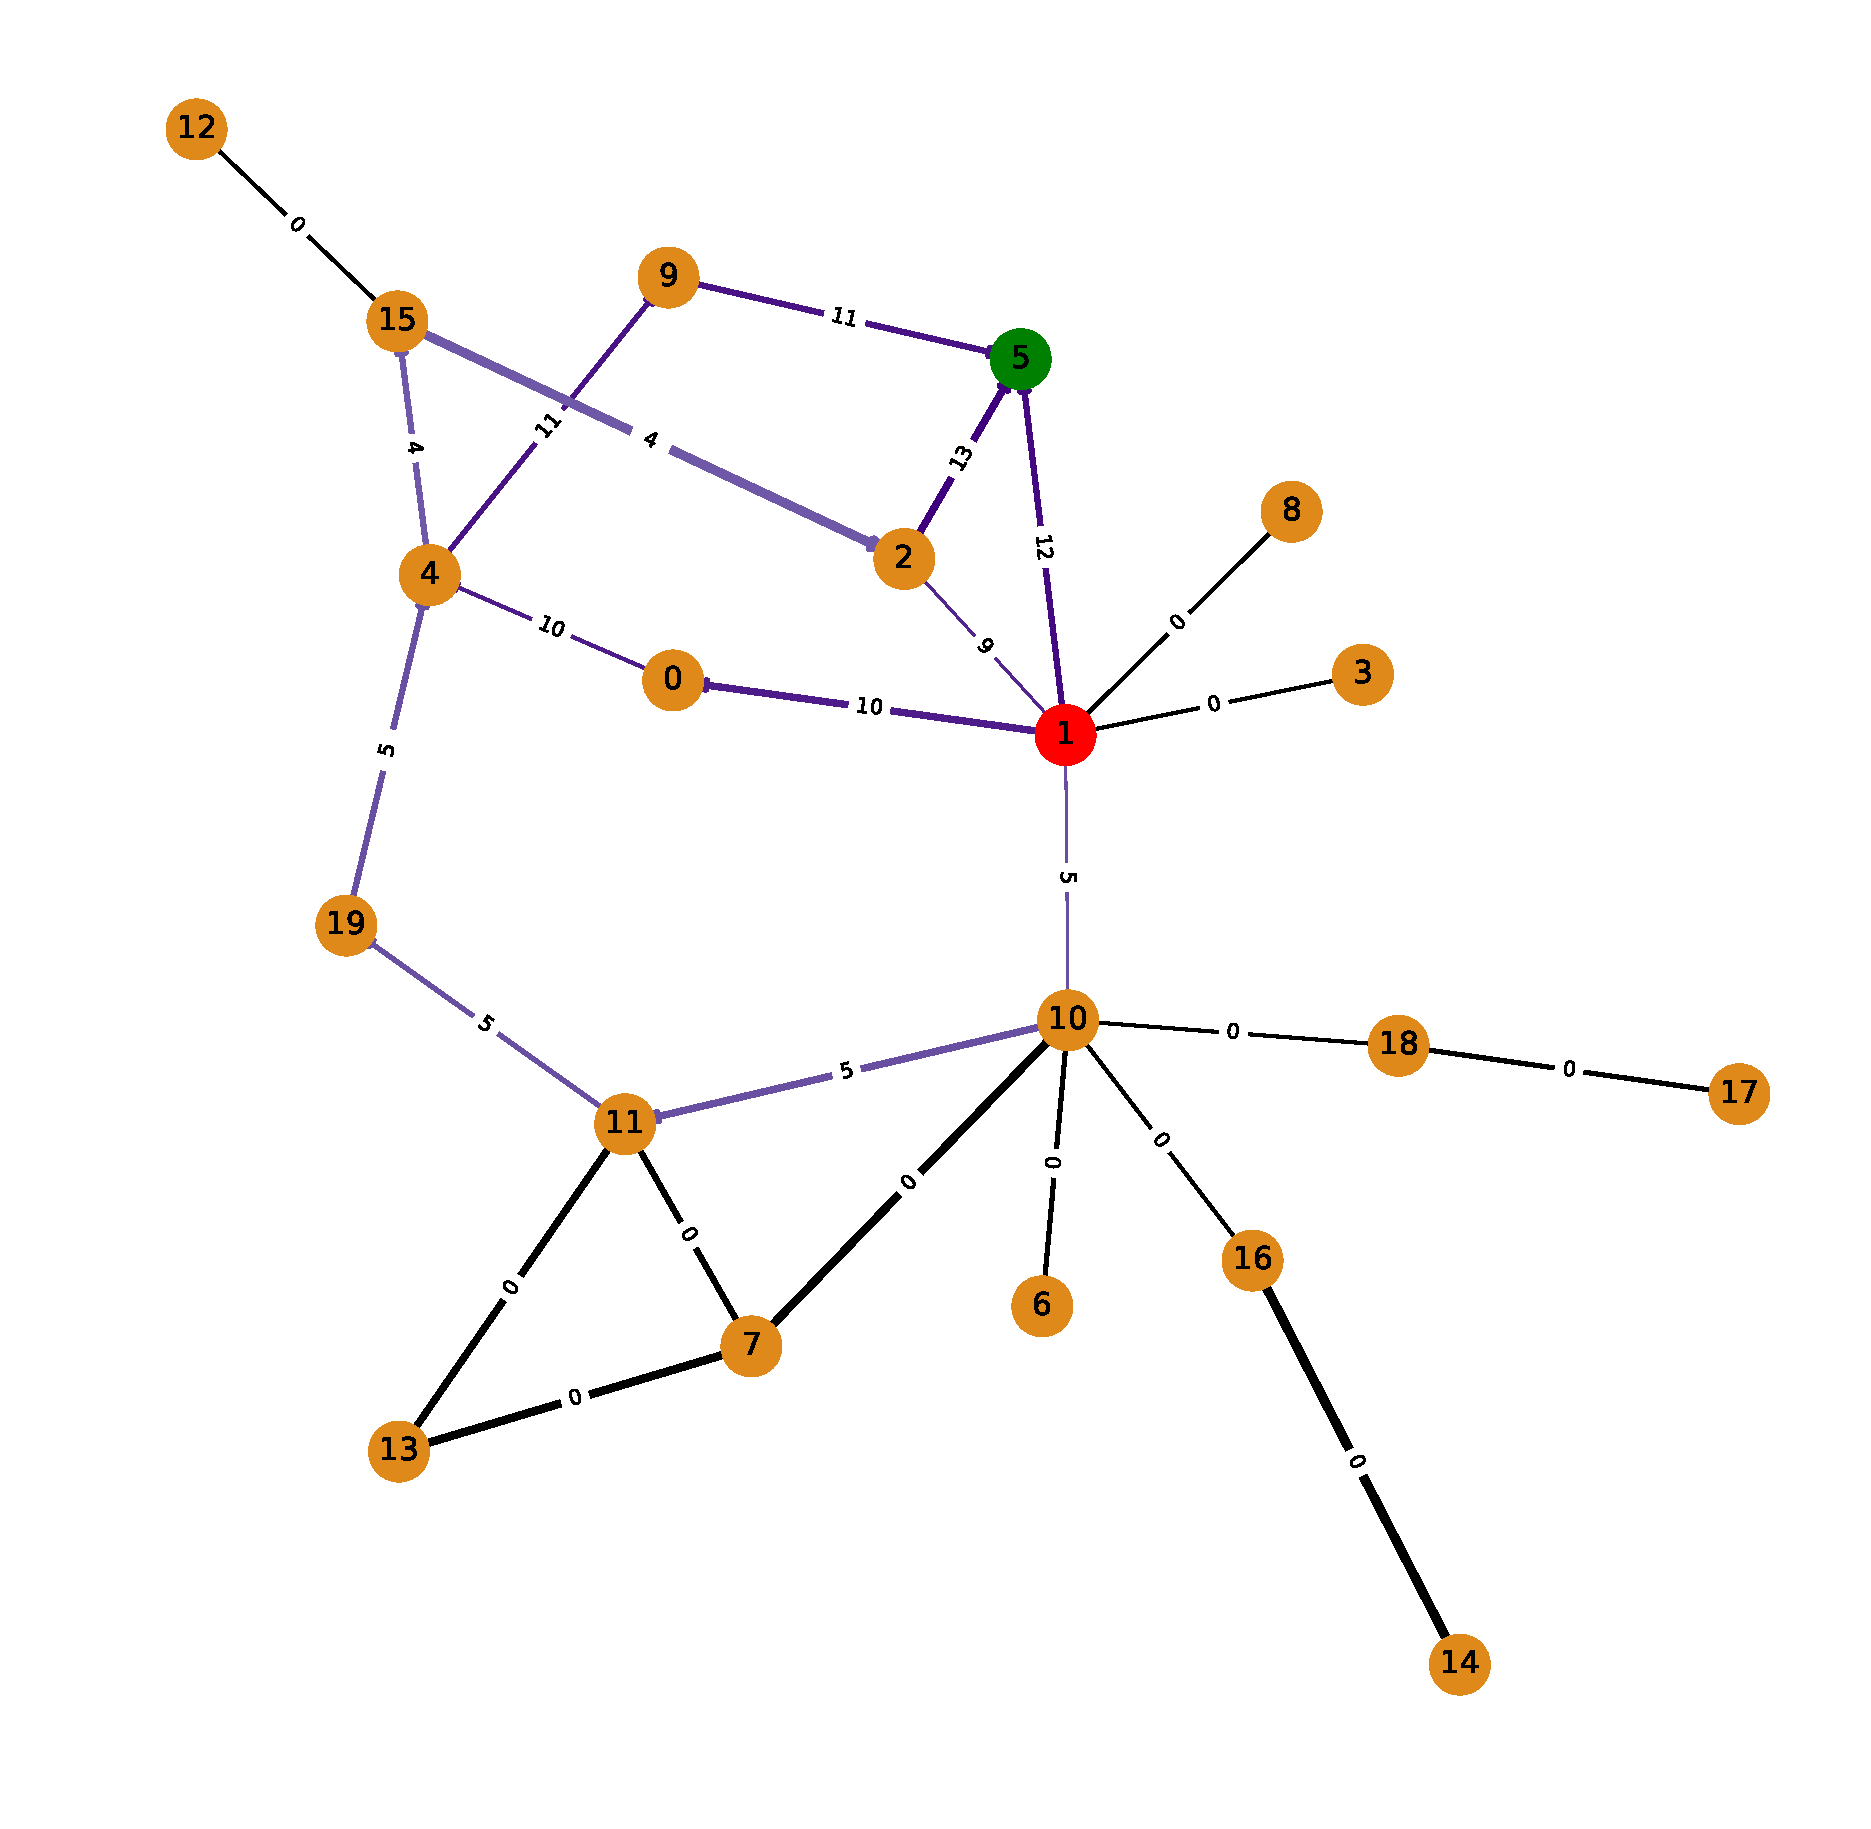
\includegraphics[scale=0.22]{Grafo2cf.eps}}
\subfigure[\textit{Grafo2}, flujo máximo 39]{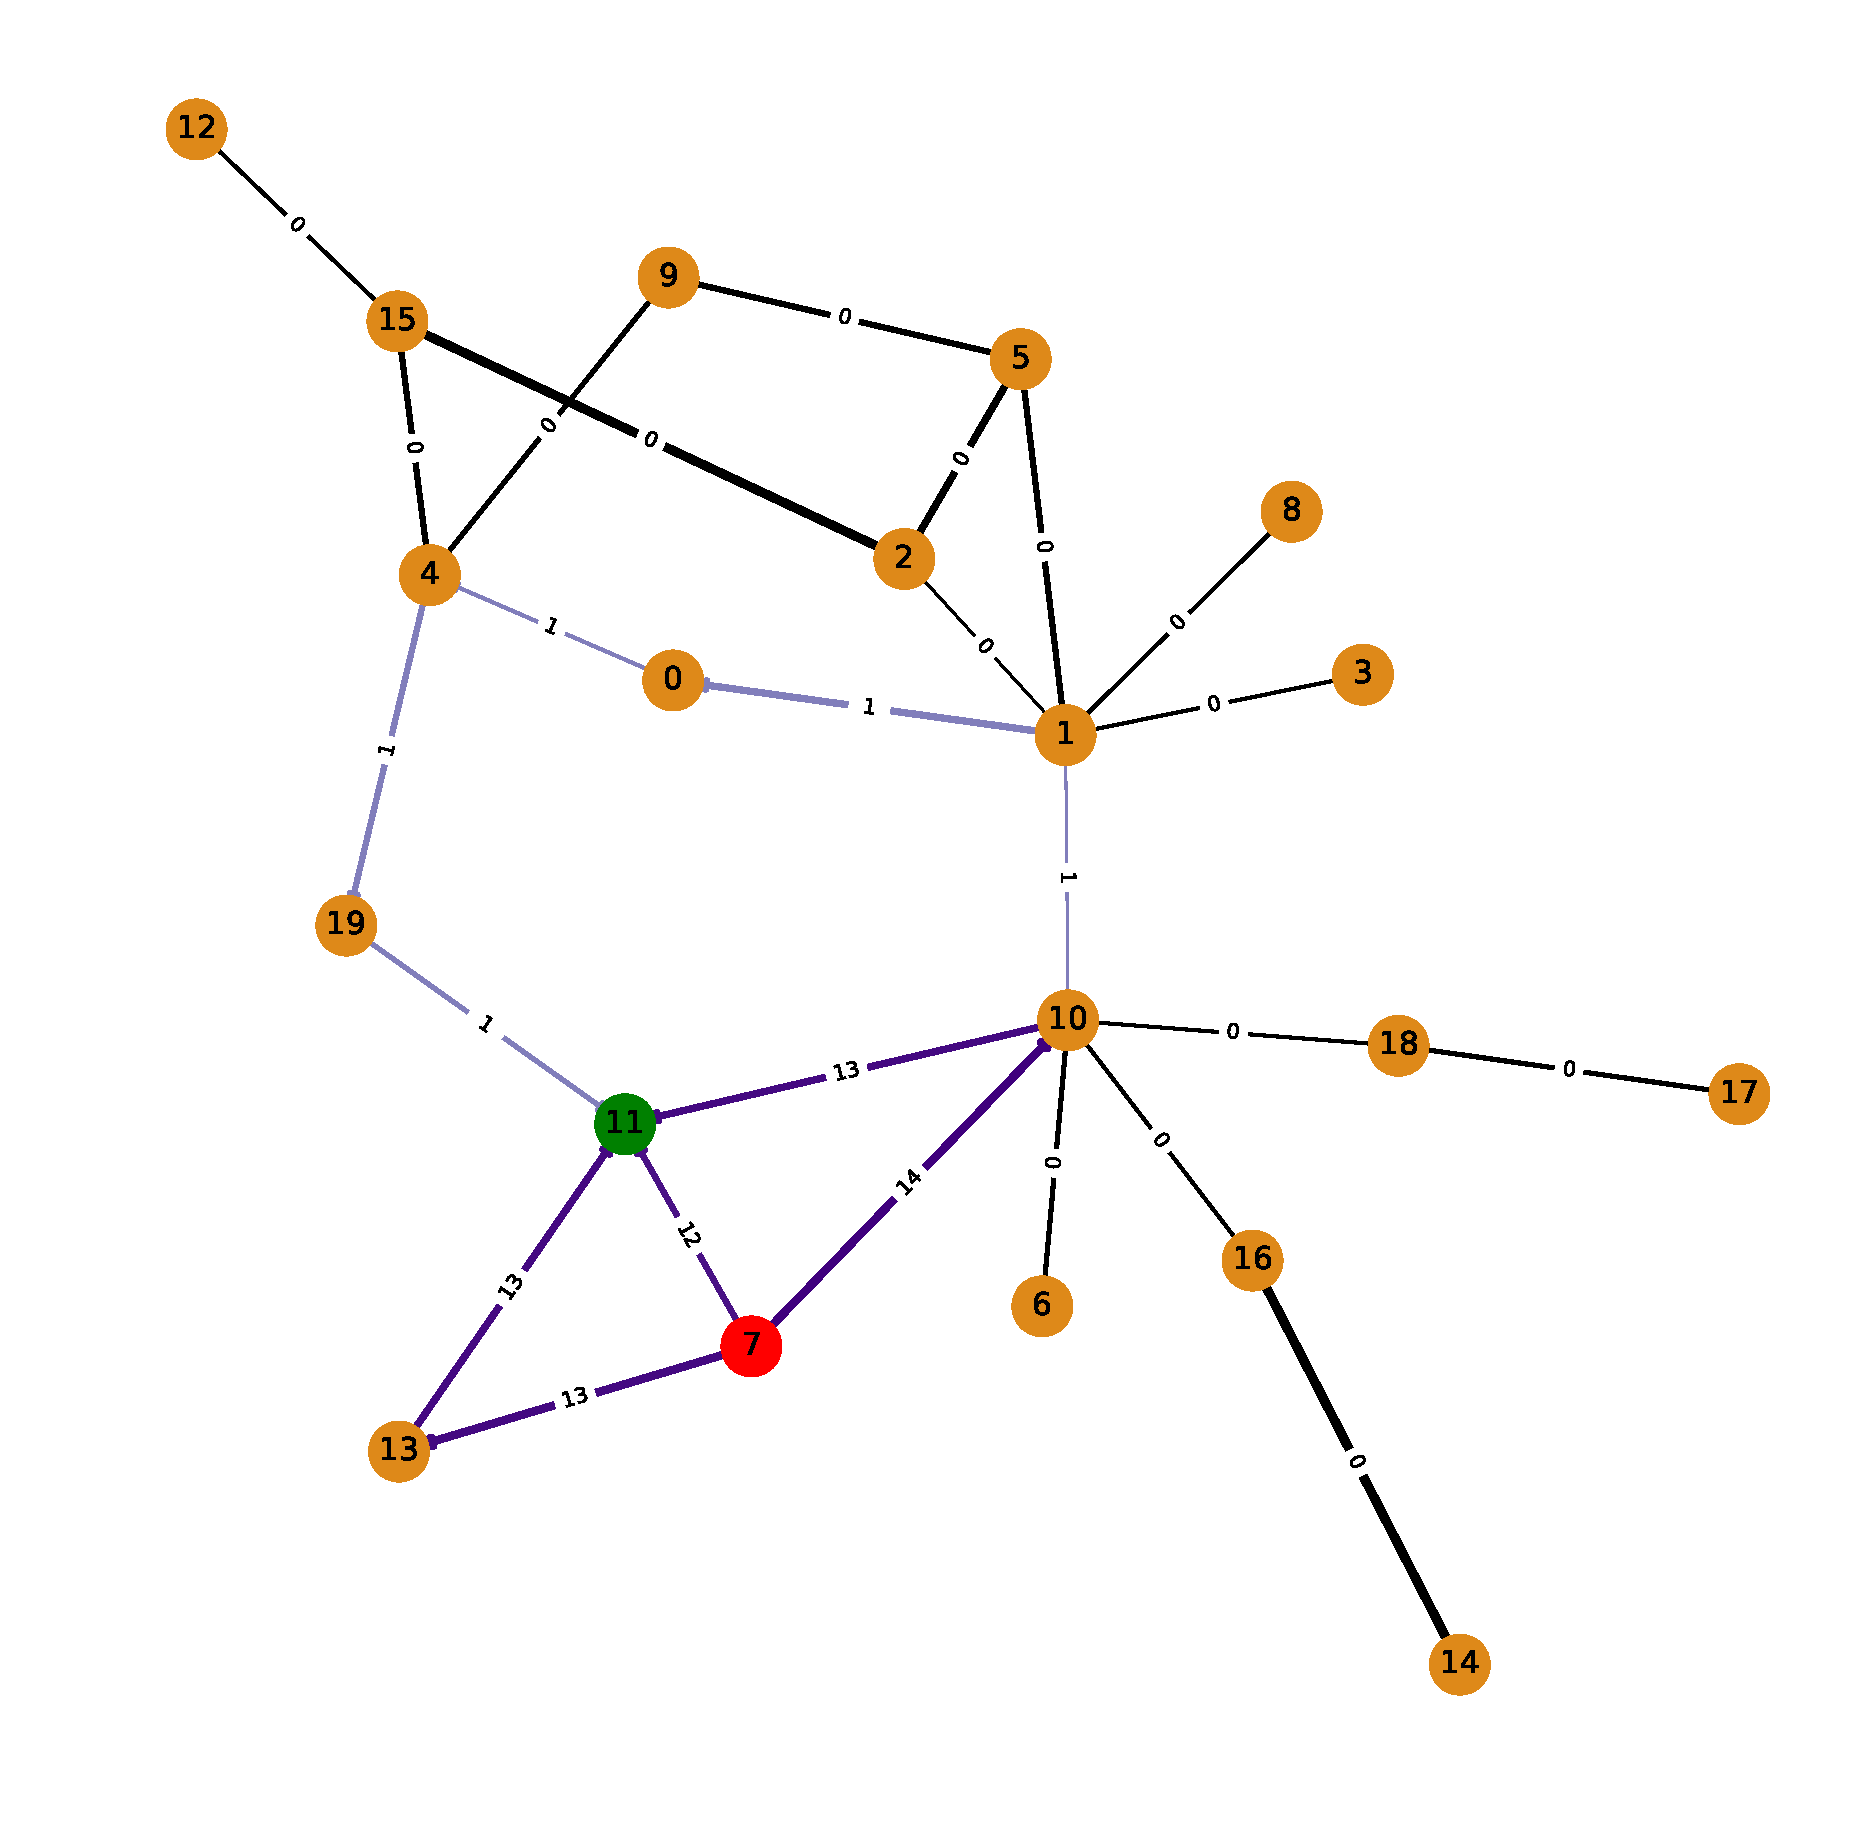
\includegraphics[scale=0.22]{Grafo2bf.eps}}
\subfigure[\textit{Grafo2}, flujo máximo 40]{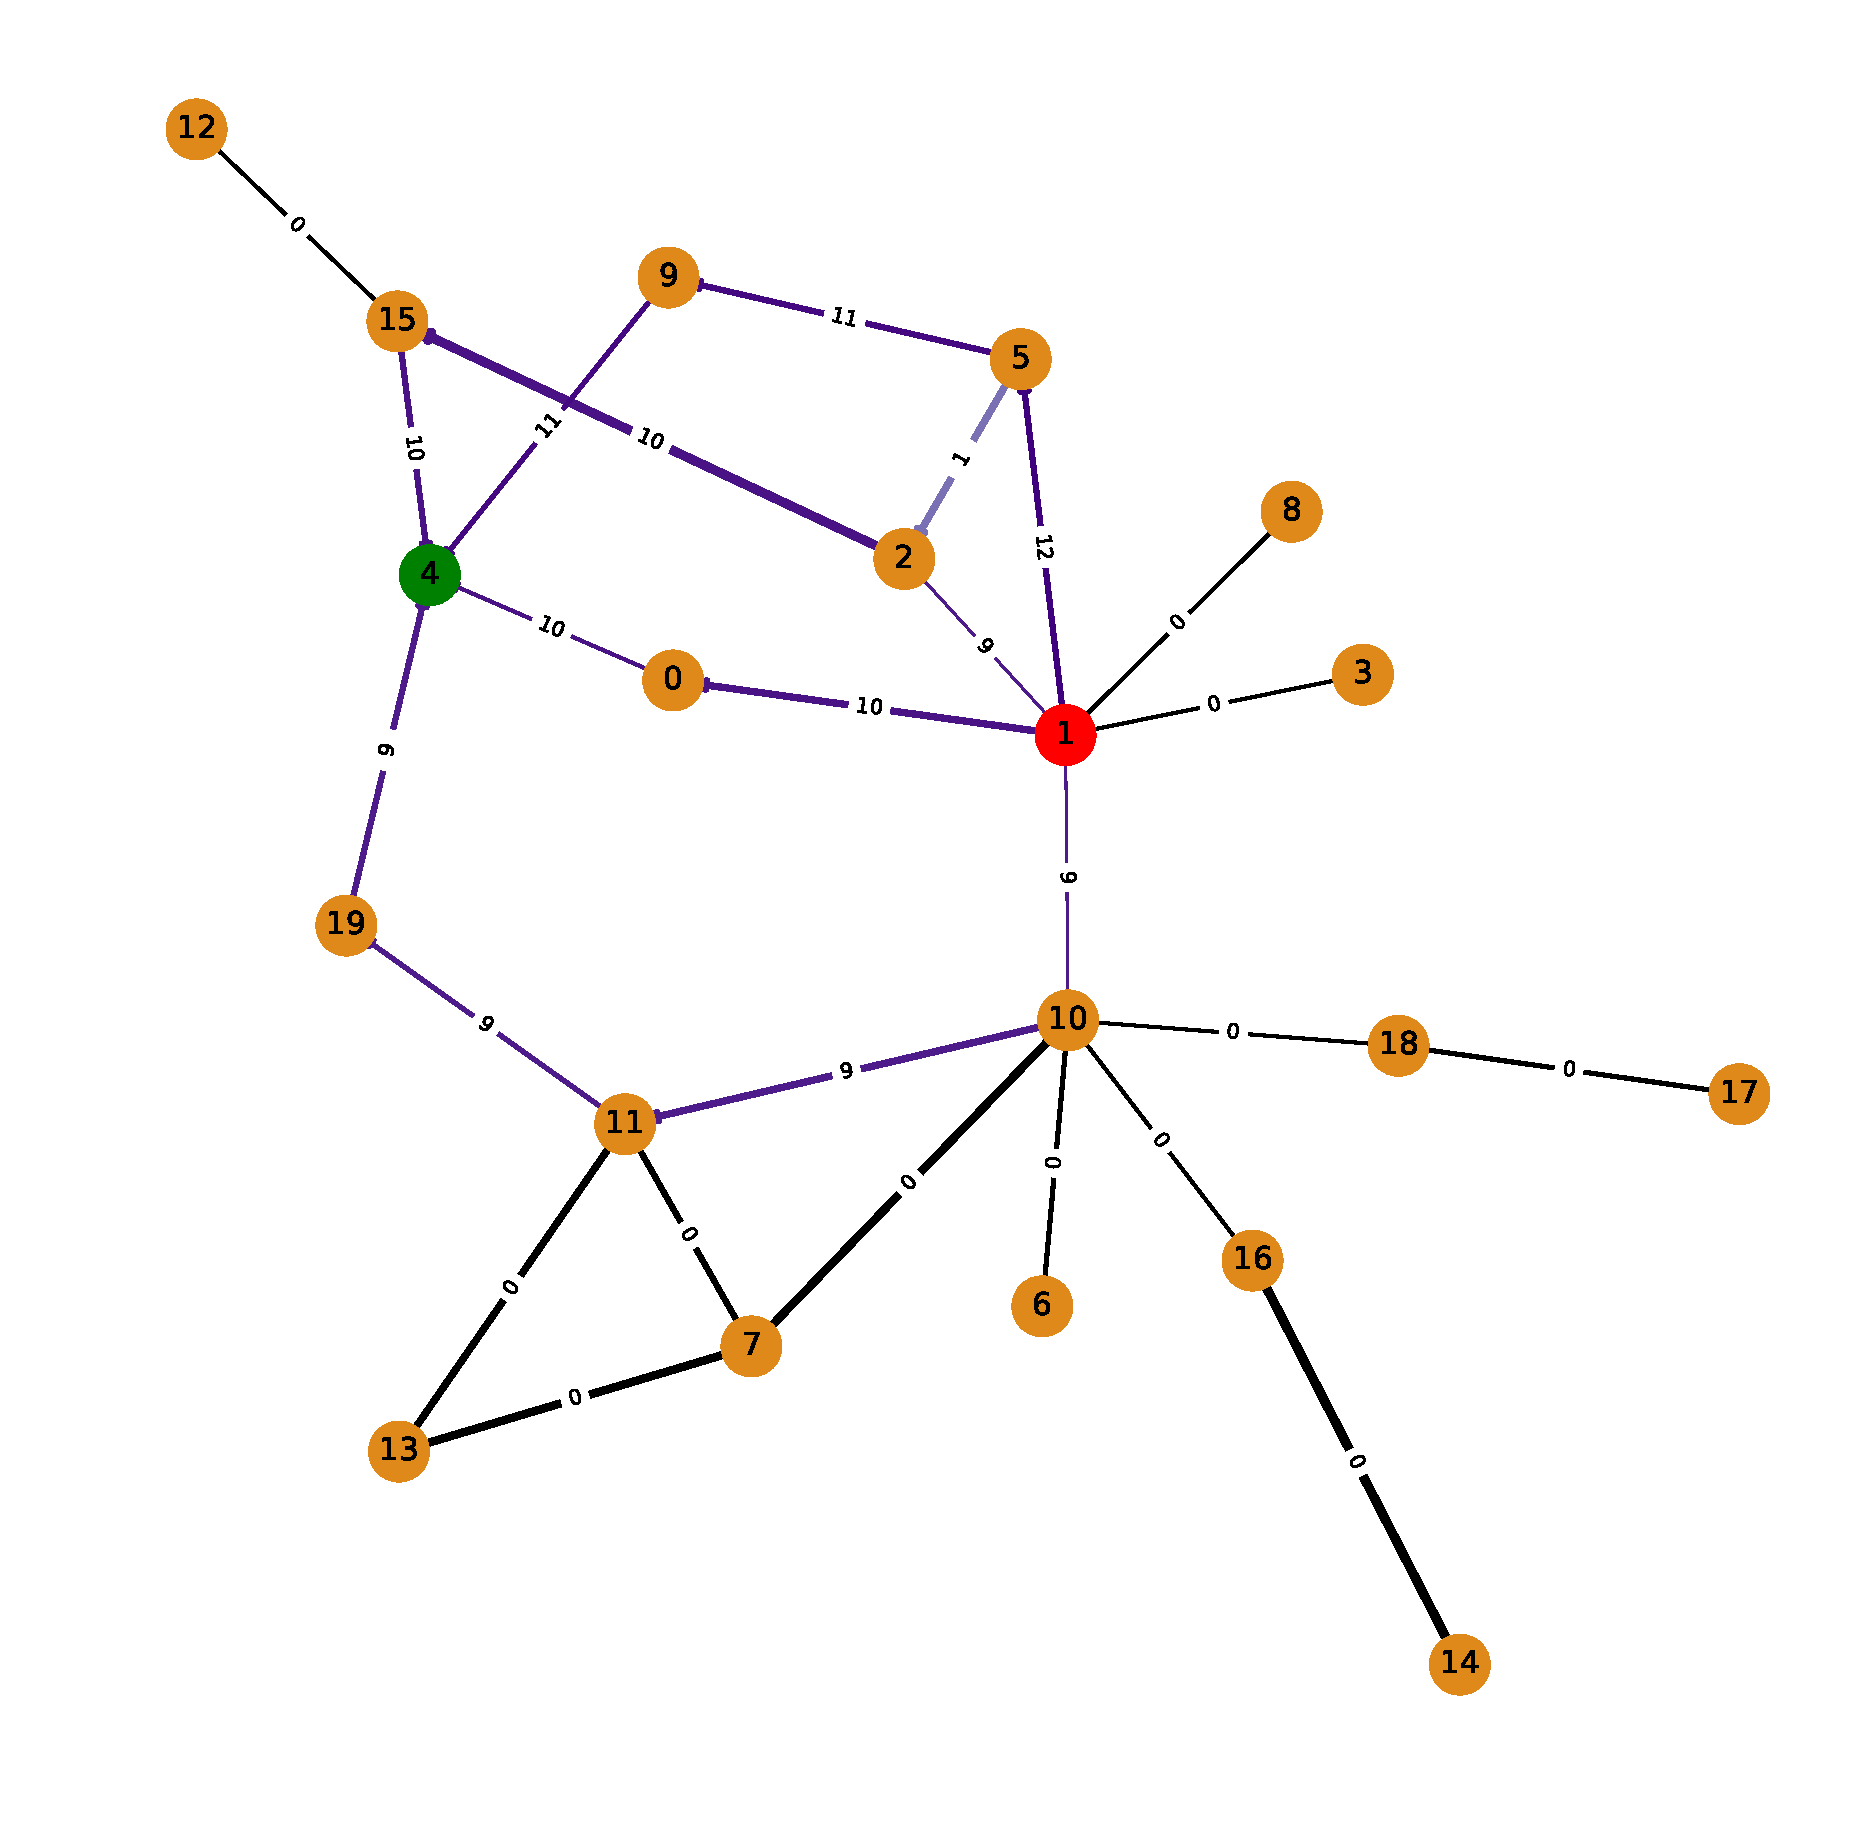
\includegraphics[scale=0.32]{Grafo2af.eps}}

\caption{Grafos resultantes de la aplicación del algoritmo de flujo máximo, donde el grosor de las aristas representa la capacidad de las mismas, el color negro la ausencia de flujo, el color violeta la presencia de flujo y la intensidad del color violeta la cantidad de flujo que pasa por la arista. El color rojo del vértice representa la fuente y el vértice verde el sumidero. }
\label{fig3} 
\end{figure}

Para el Grafo3 esto se muestra en la figura \ref{fig4} de la página \pageref{fig4}.

\begin{figure}[htbp]

\subfigure[\textit{Grafo3}, flujo máximo 10]{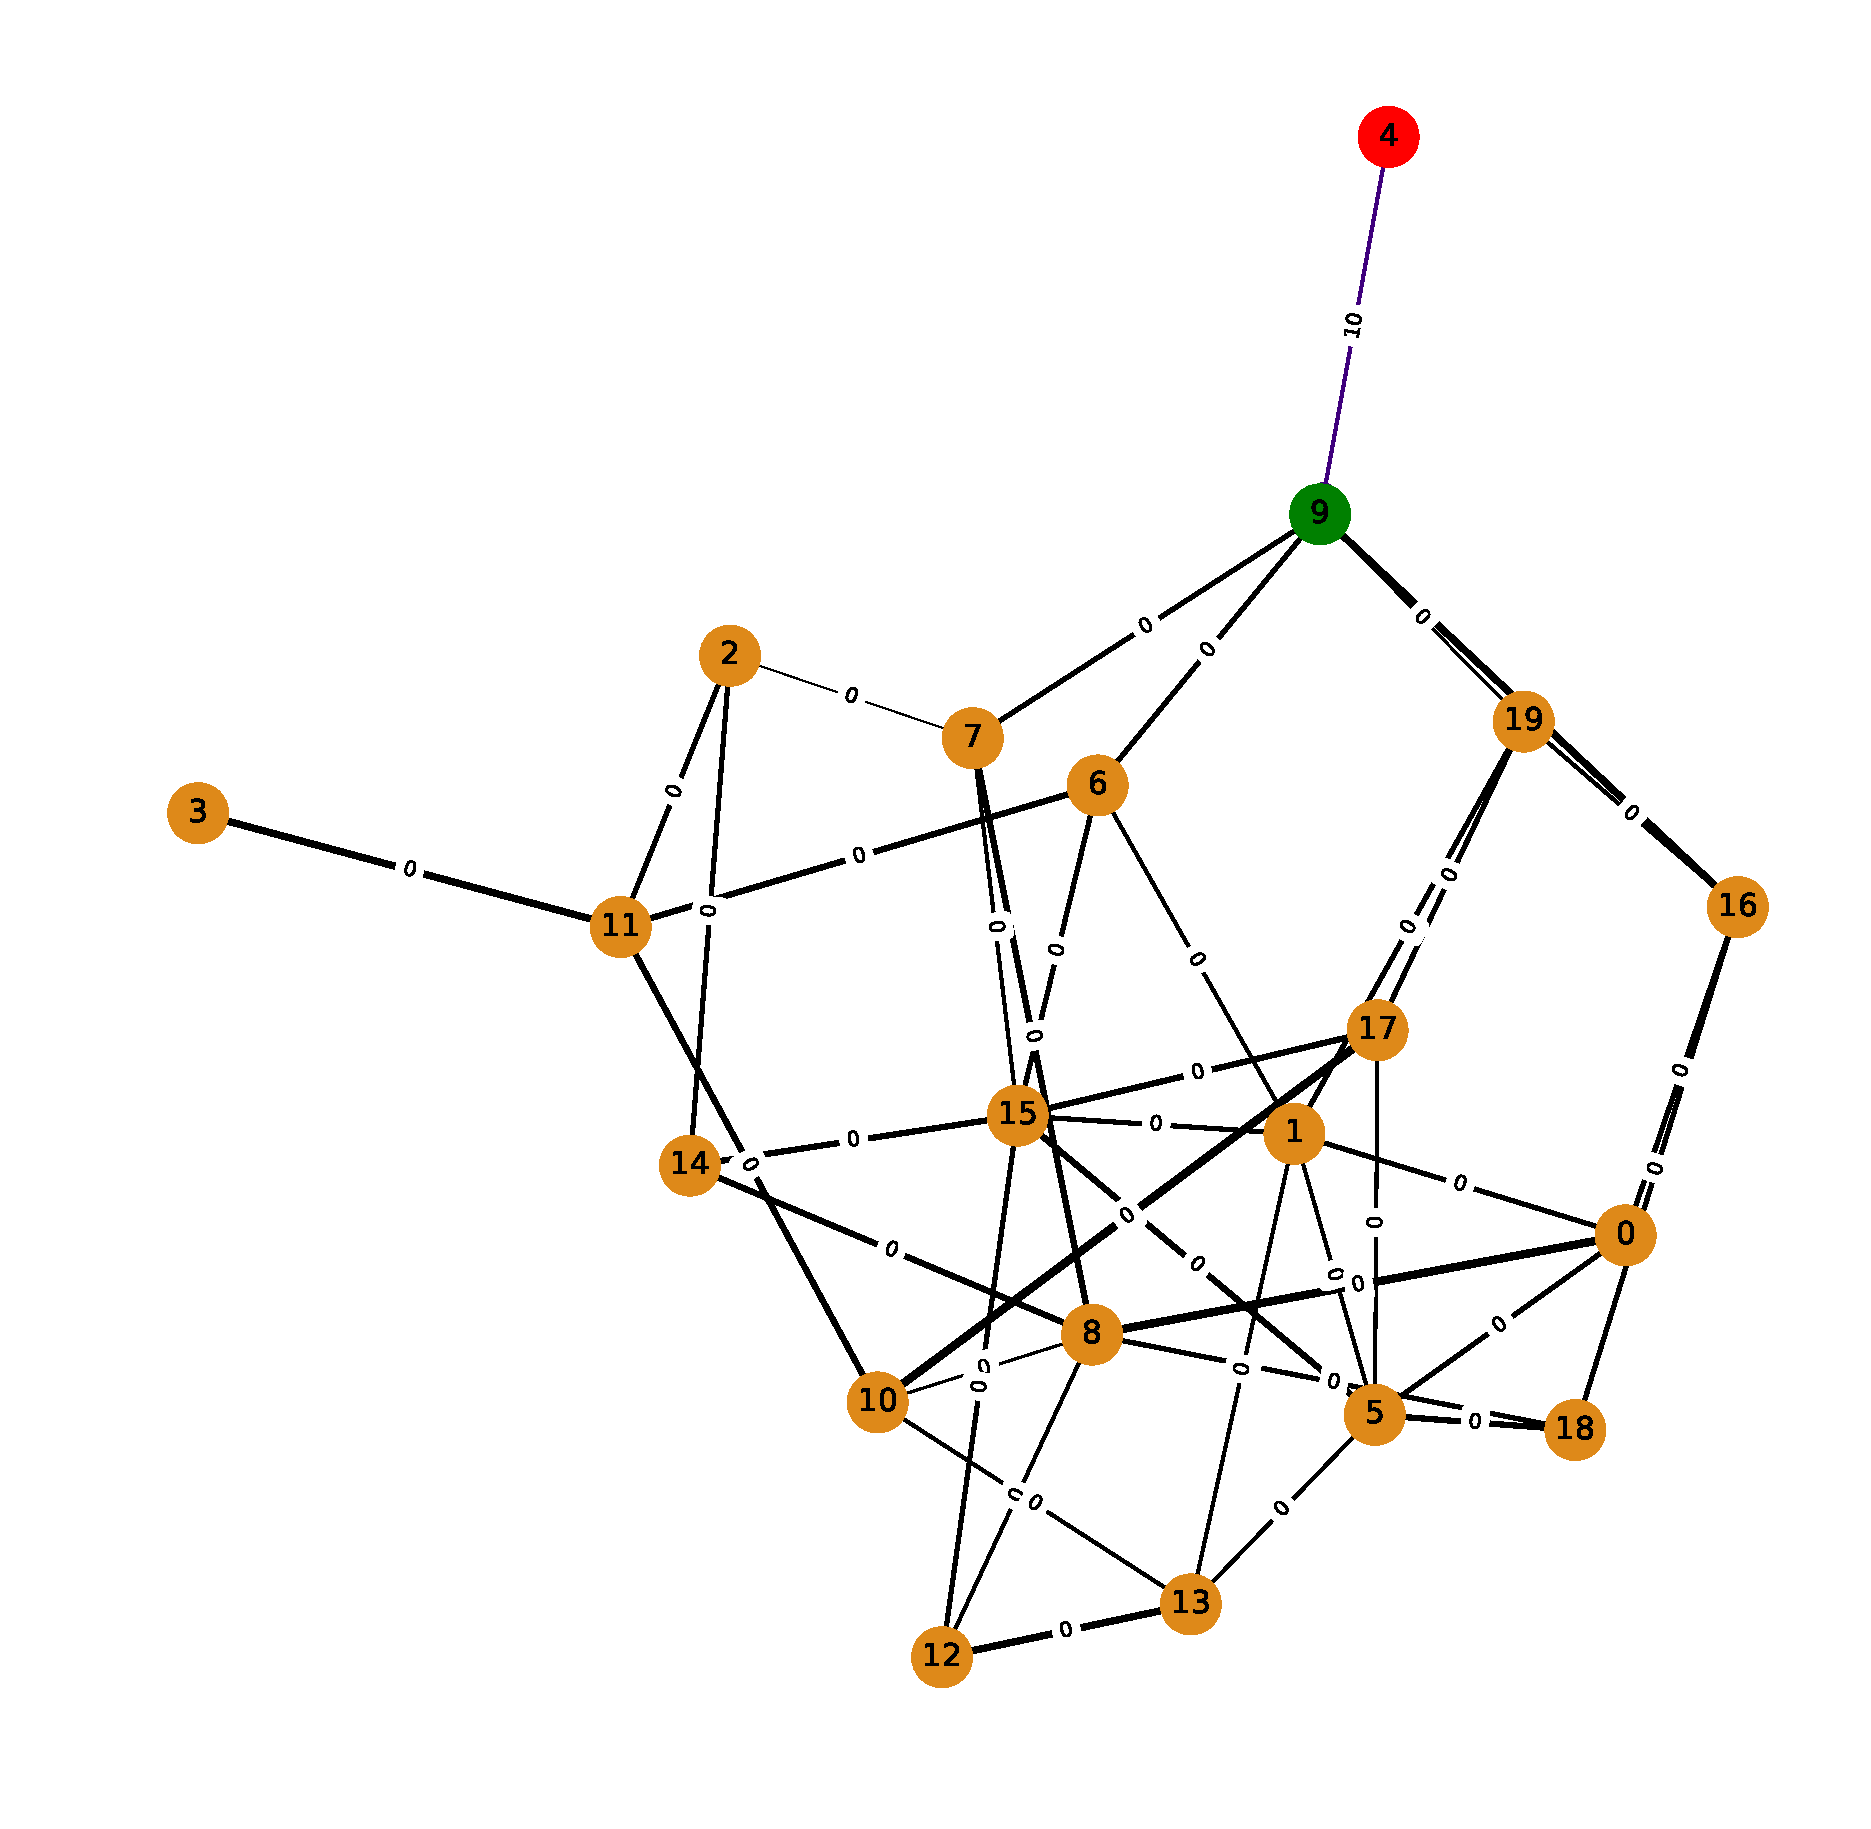
\includegraphics[scale=0.22]{Grafo3mf.eps}}
\subfigure[\textit{Grafo3}, flujo máximo 41]{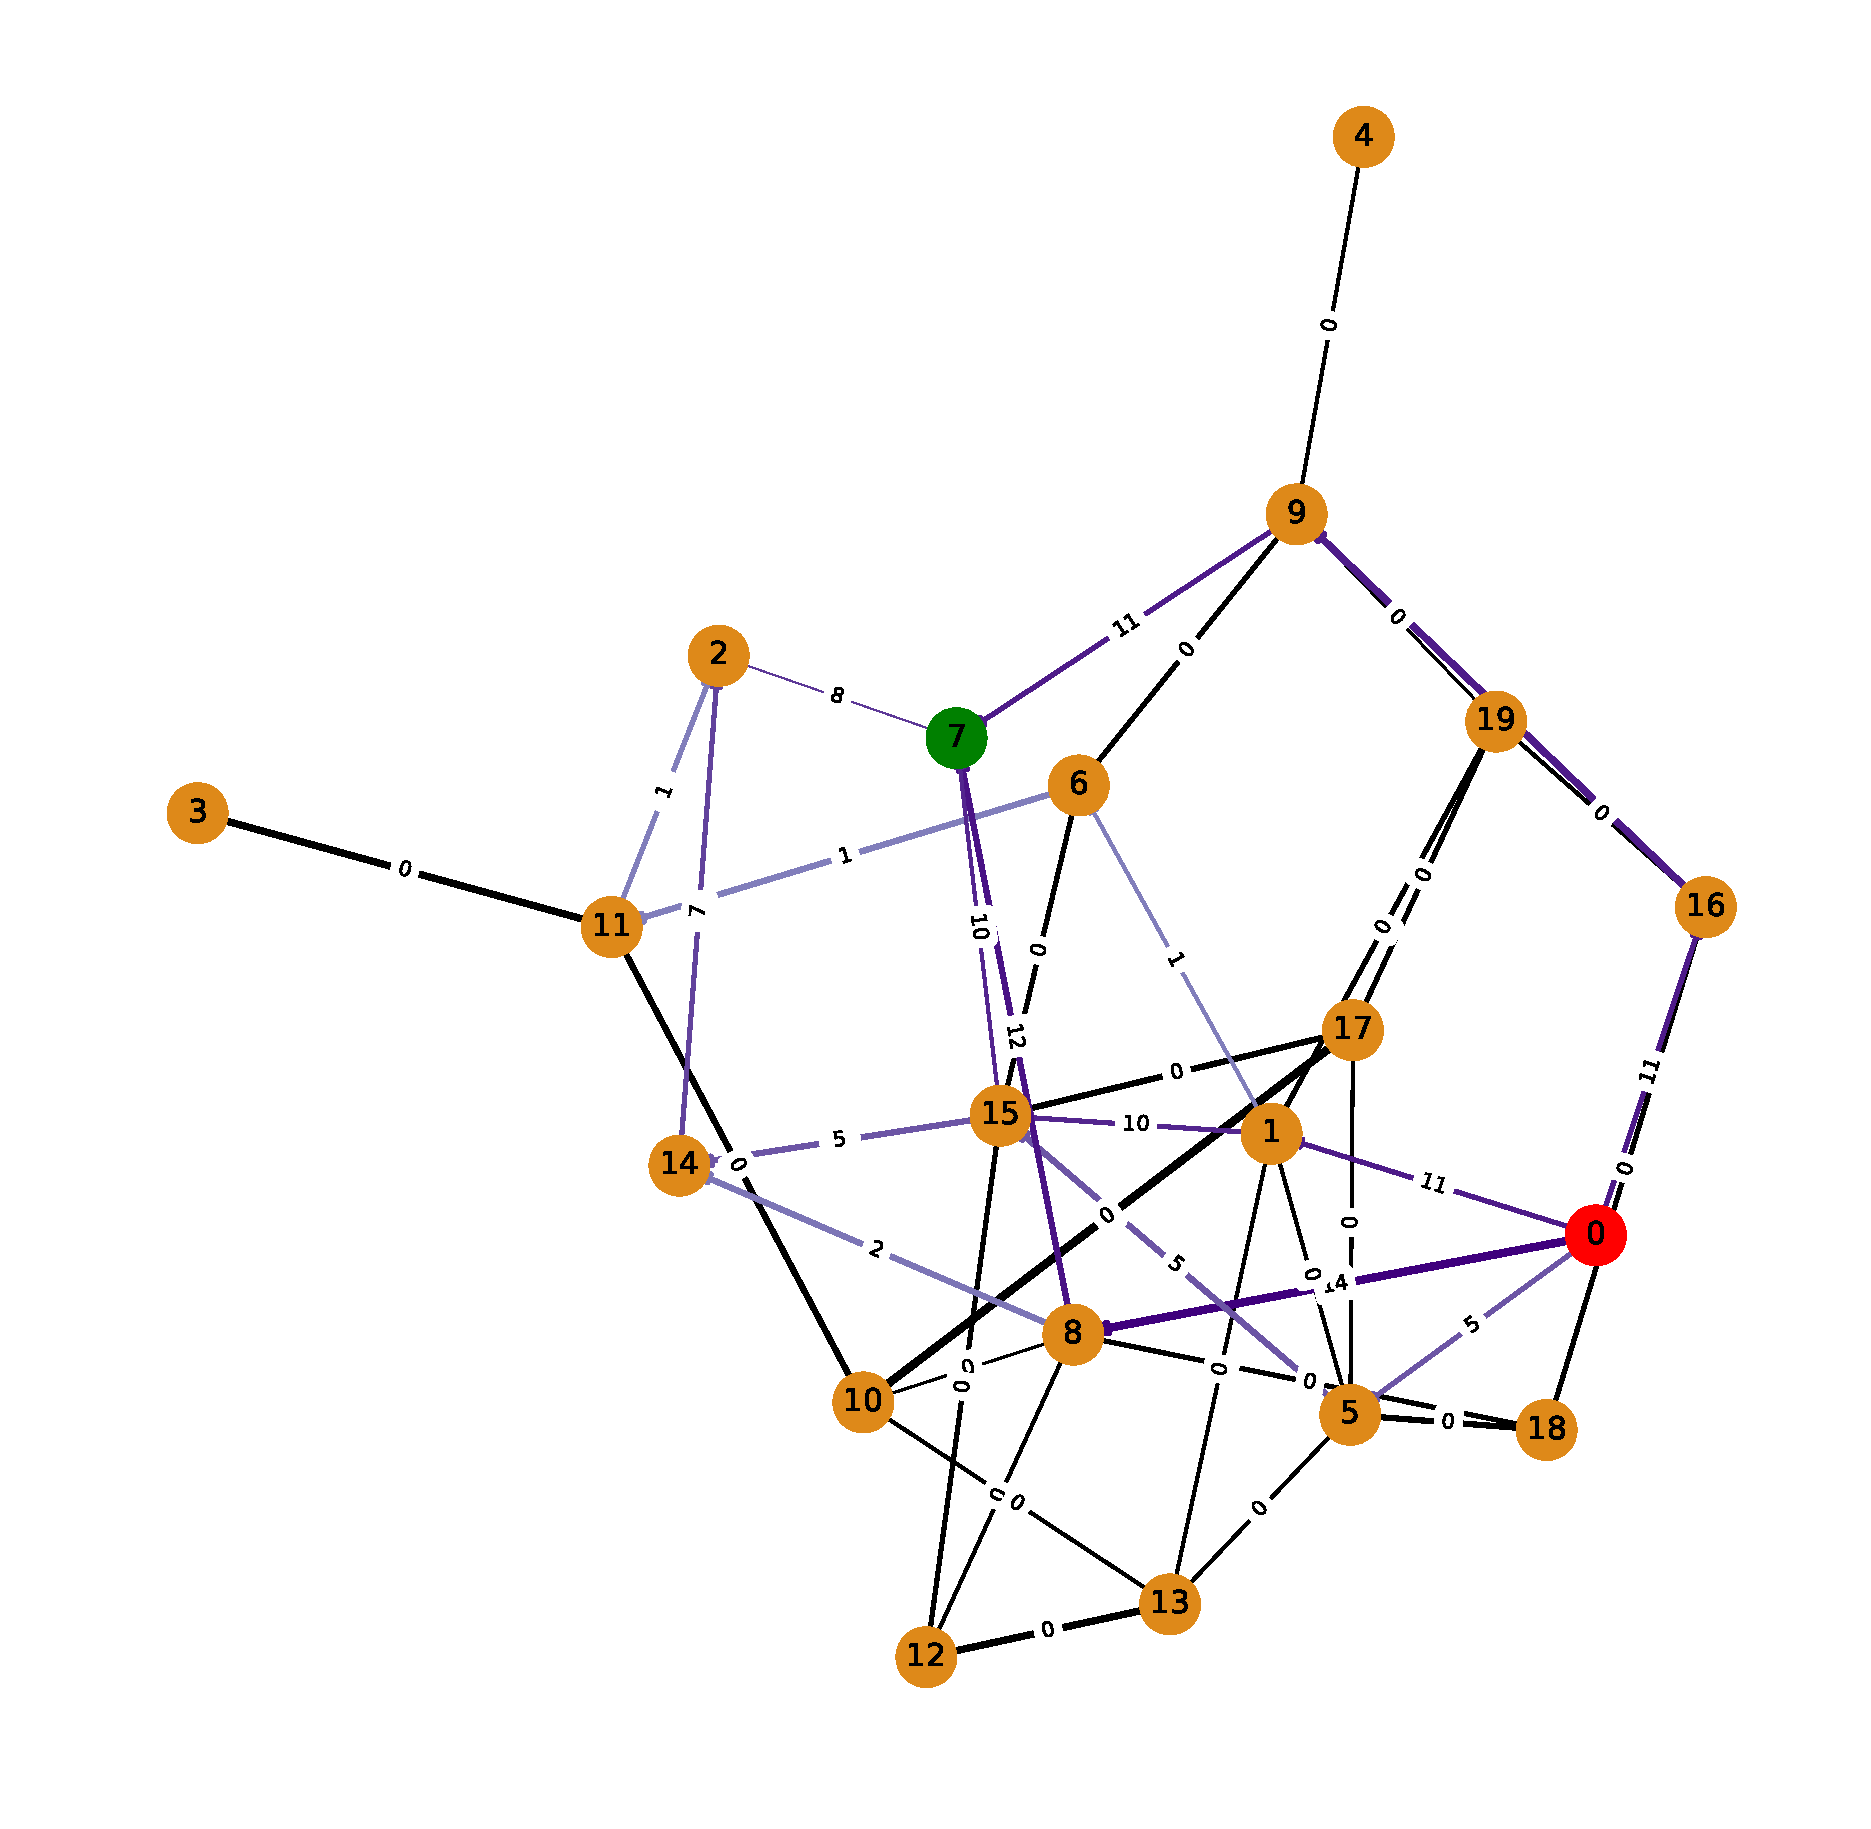
\includegraphics[scale=0.22]{Grafo3cf.eps}}
\subfigure[\textit{Grafo3}, flujo máximo 65]{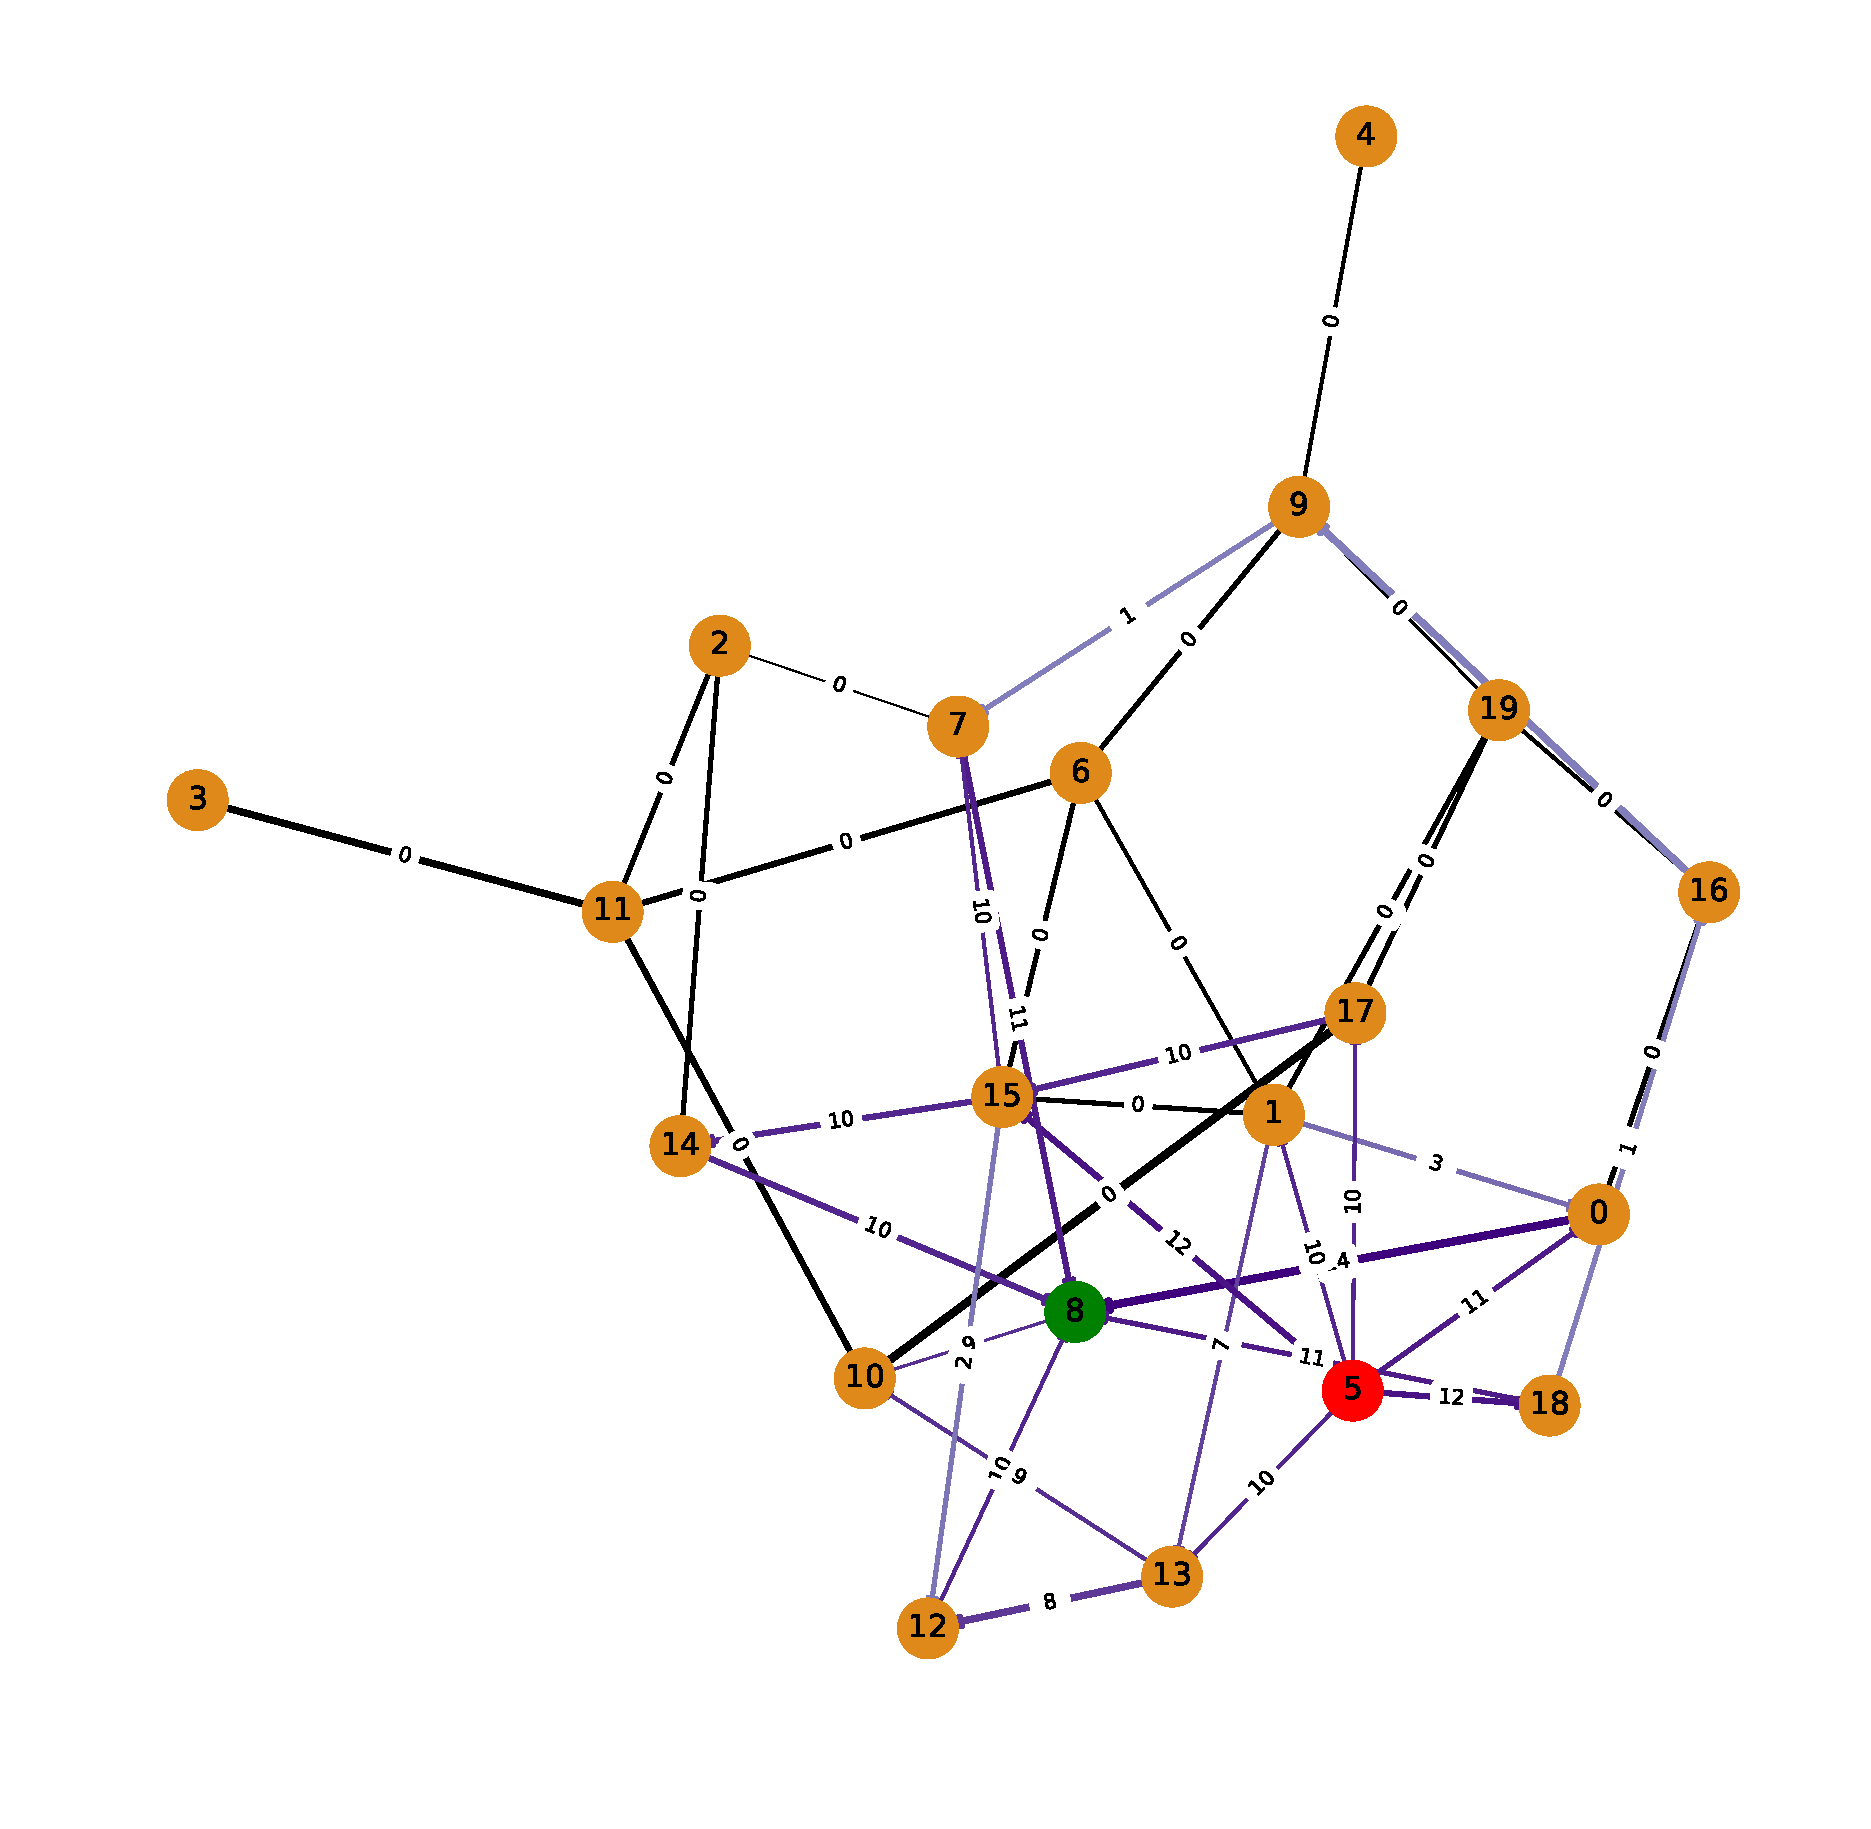
\includegraphics[scale=0.22]{Grafo3bf.eps}}
\subfigure[\textit{Grafo3}, flujo máximo 68]{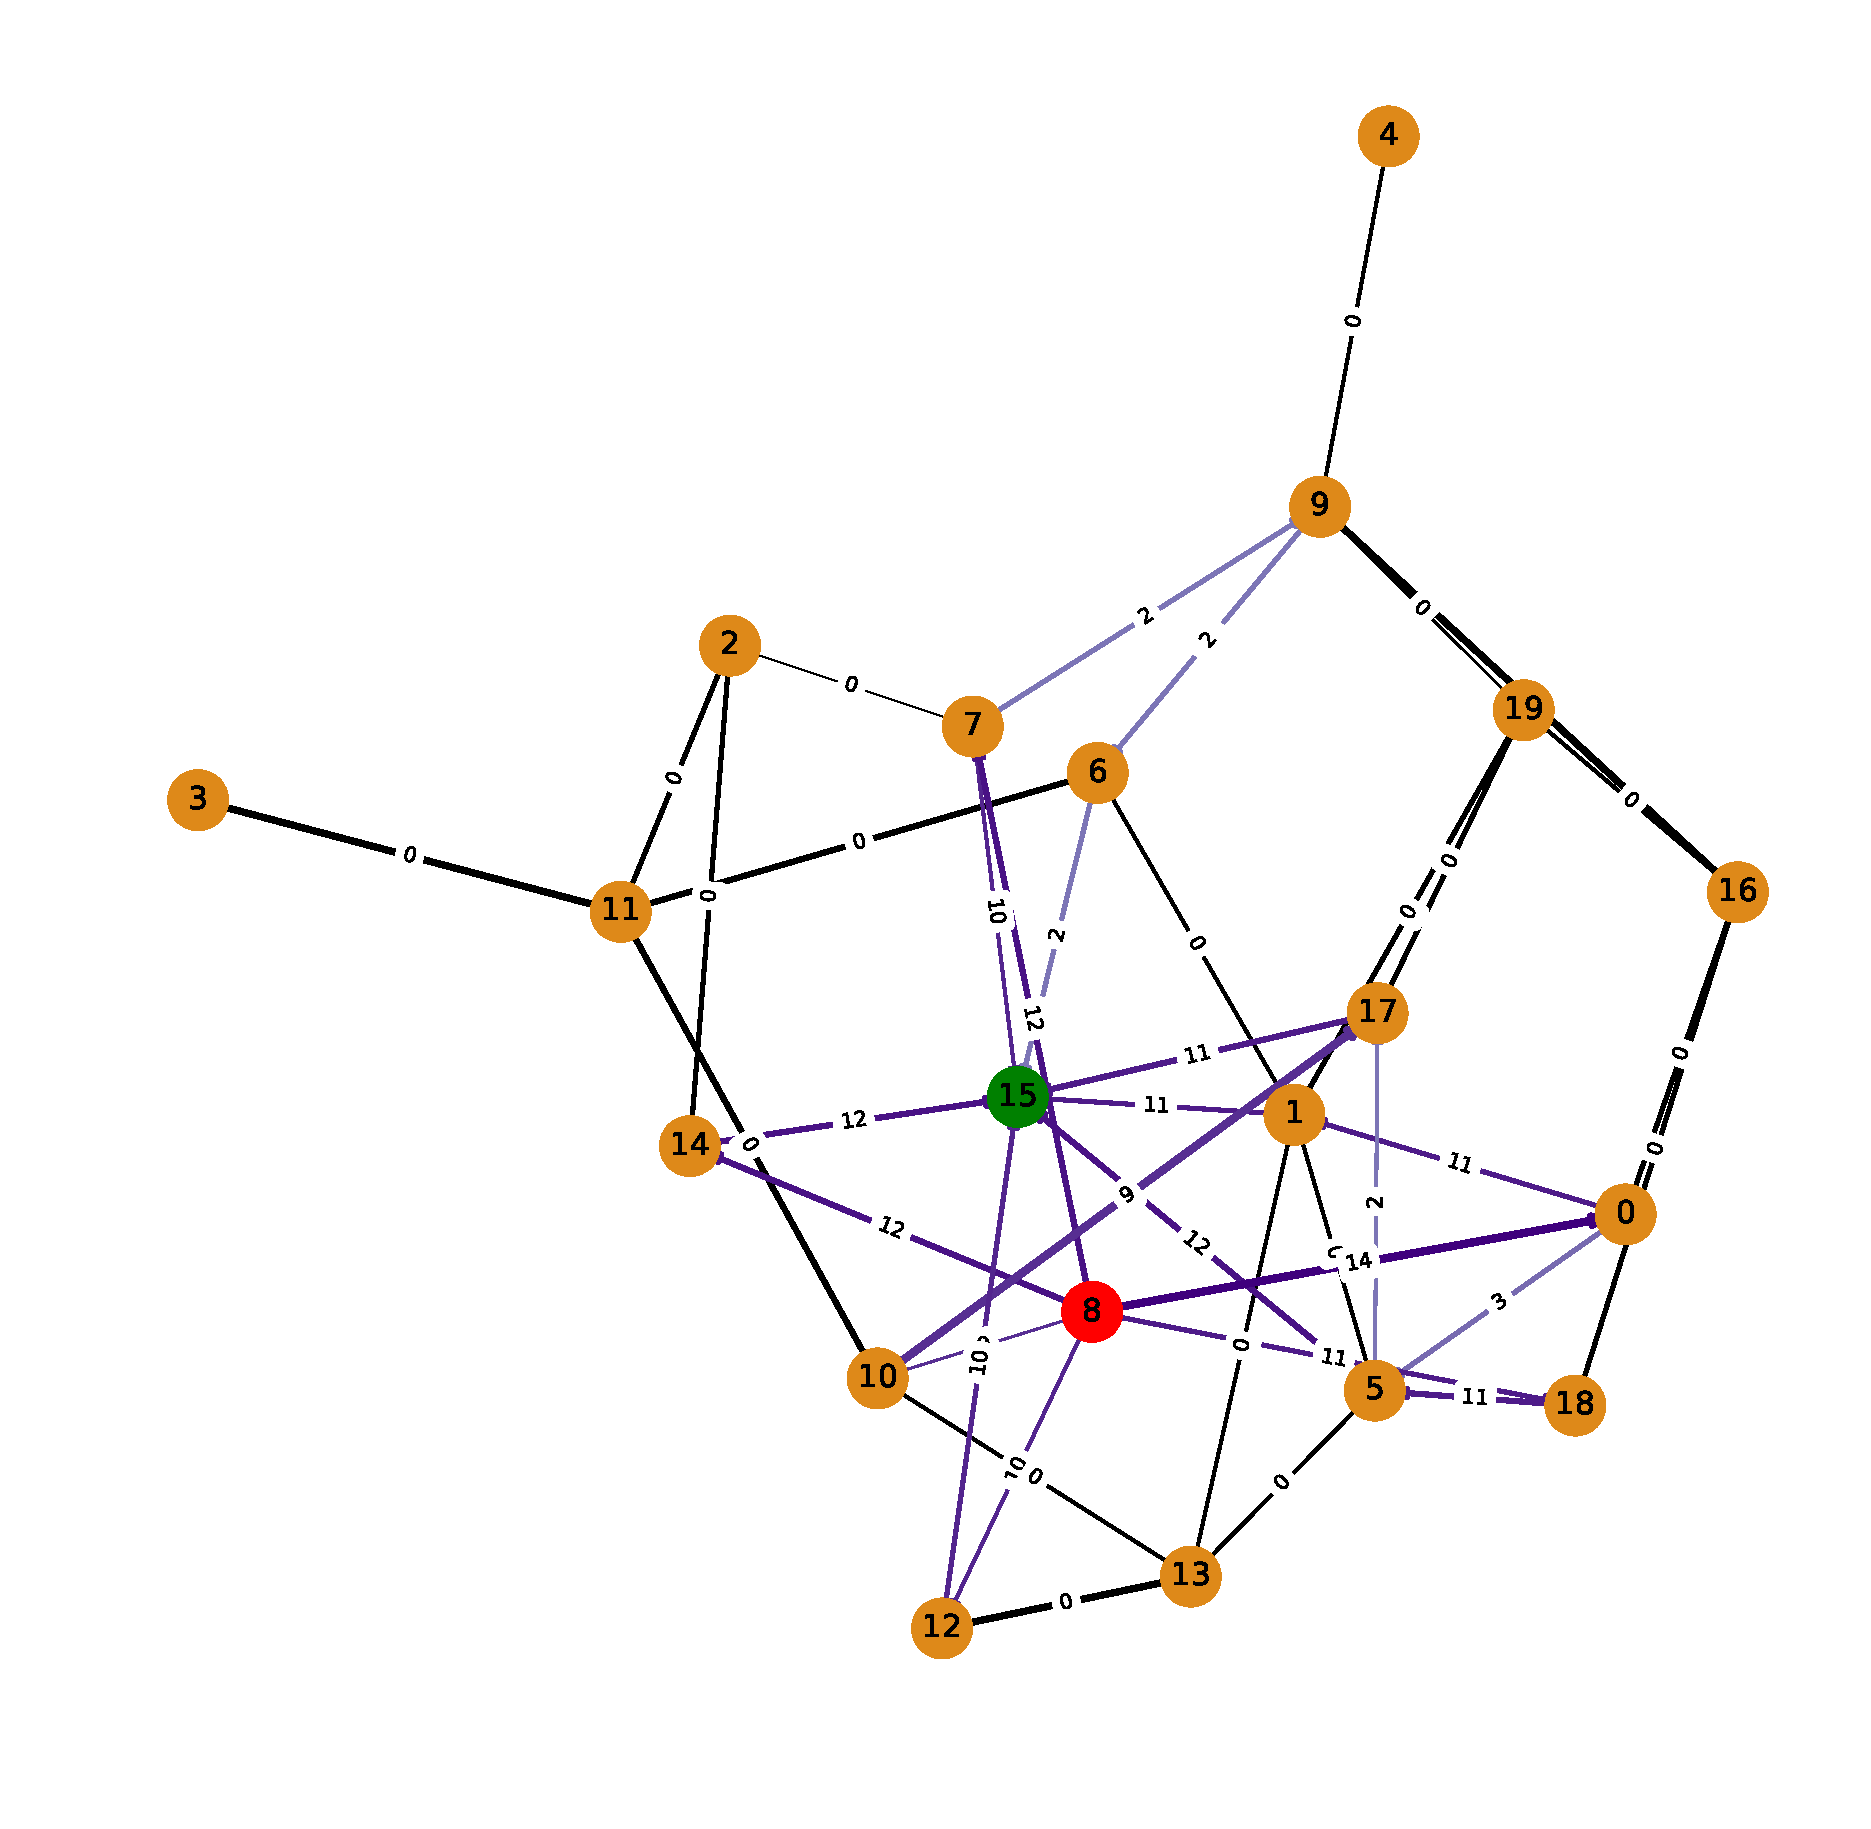
\includegraphics[scale=0.32]{Grafo3af.eps}}

\caption{Grafos resultantes de la aplicación del algoritmo de flujo máximo, donde el grosor de las aristas representa la capacidad de las mismas, el color negro la ausencia de flujo, el color violeta la presencia de flujo y la intensidad del color violeta la cantidad de flujo que pasa por la arista. El color rojo del vértice representa la fuente y el vértice verde el sumidero. }
\label{fig4} 
\end{figure}

Para el Grafo4 esto se muestra en la figura \ref{fig5} de la página \pageref{fig5}.

\begin{figure}[htbp]

\subfigure[\textit{Grafo4}, flujo máximo 32]{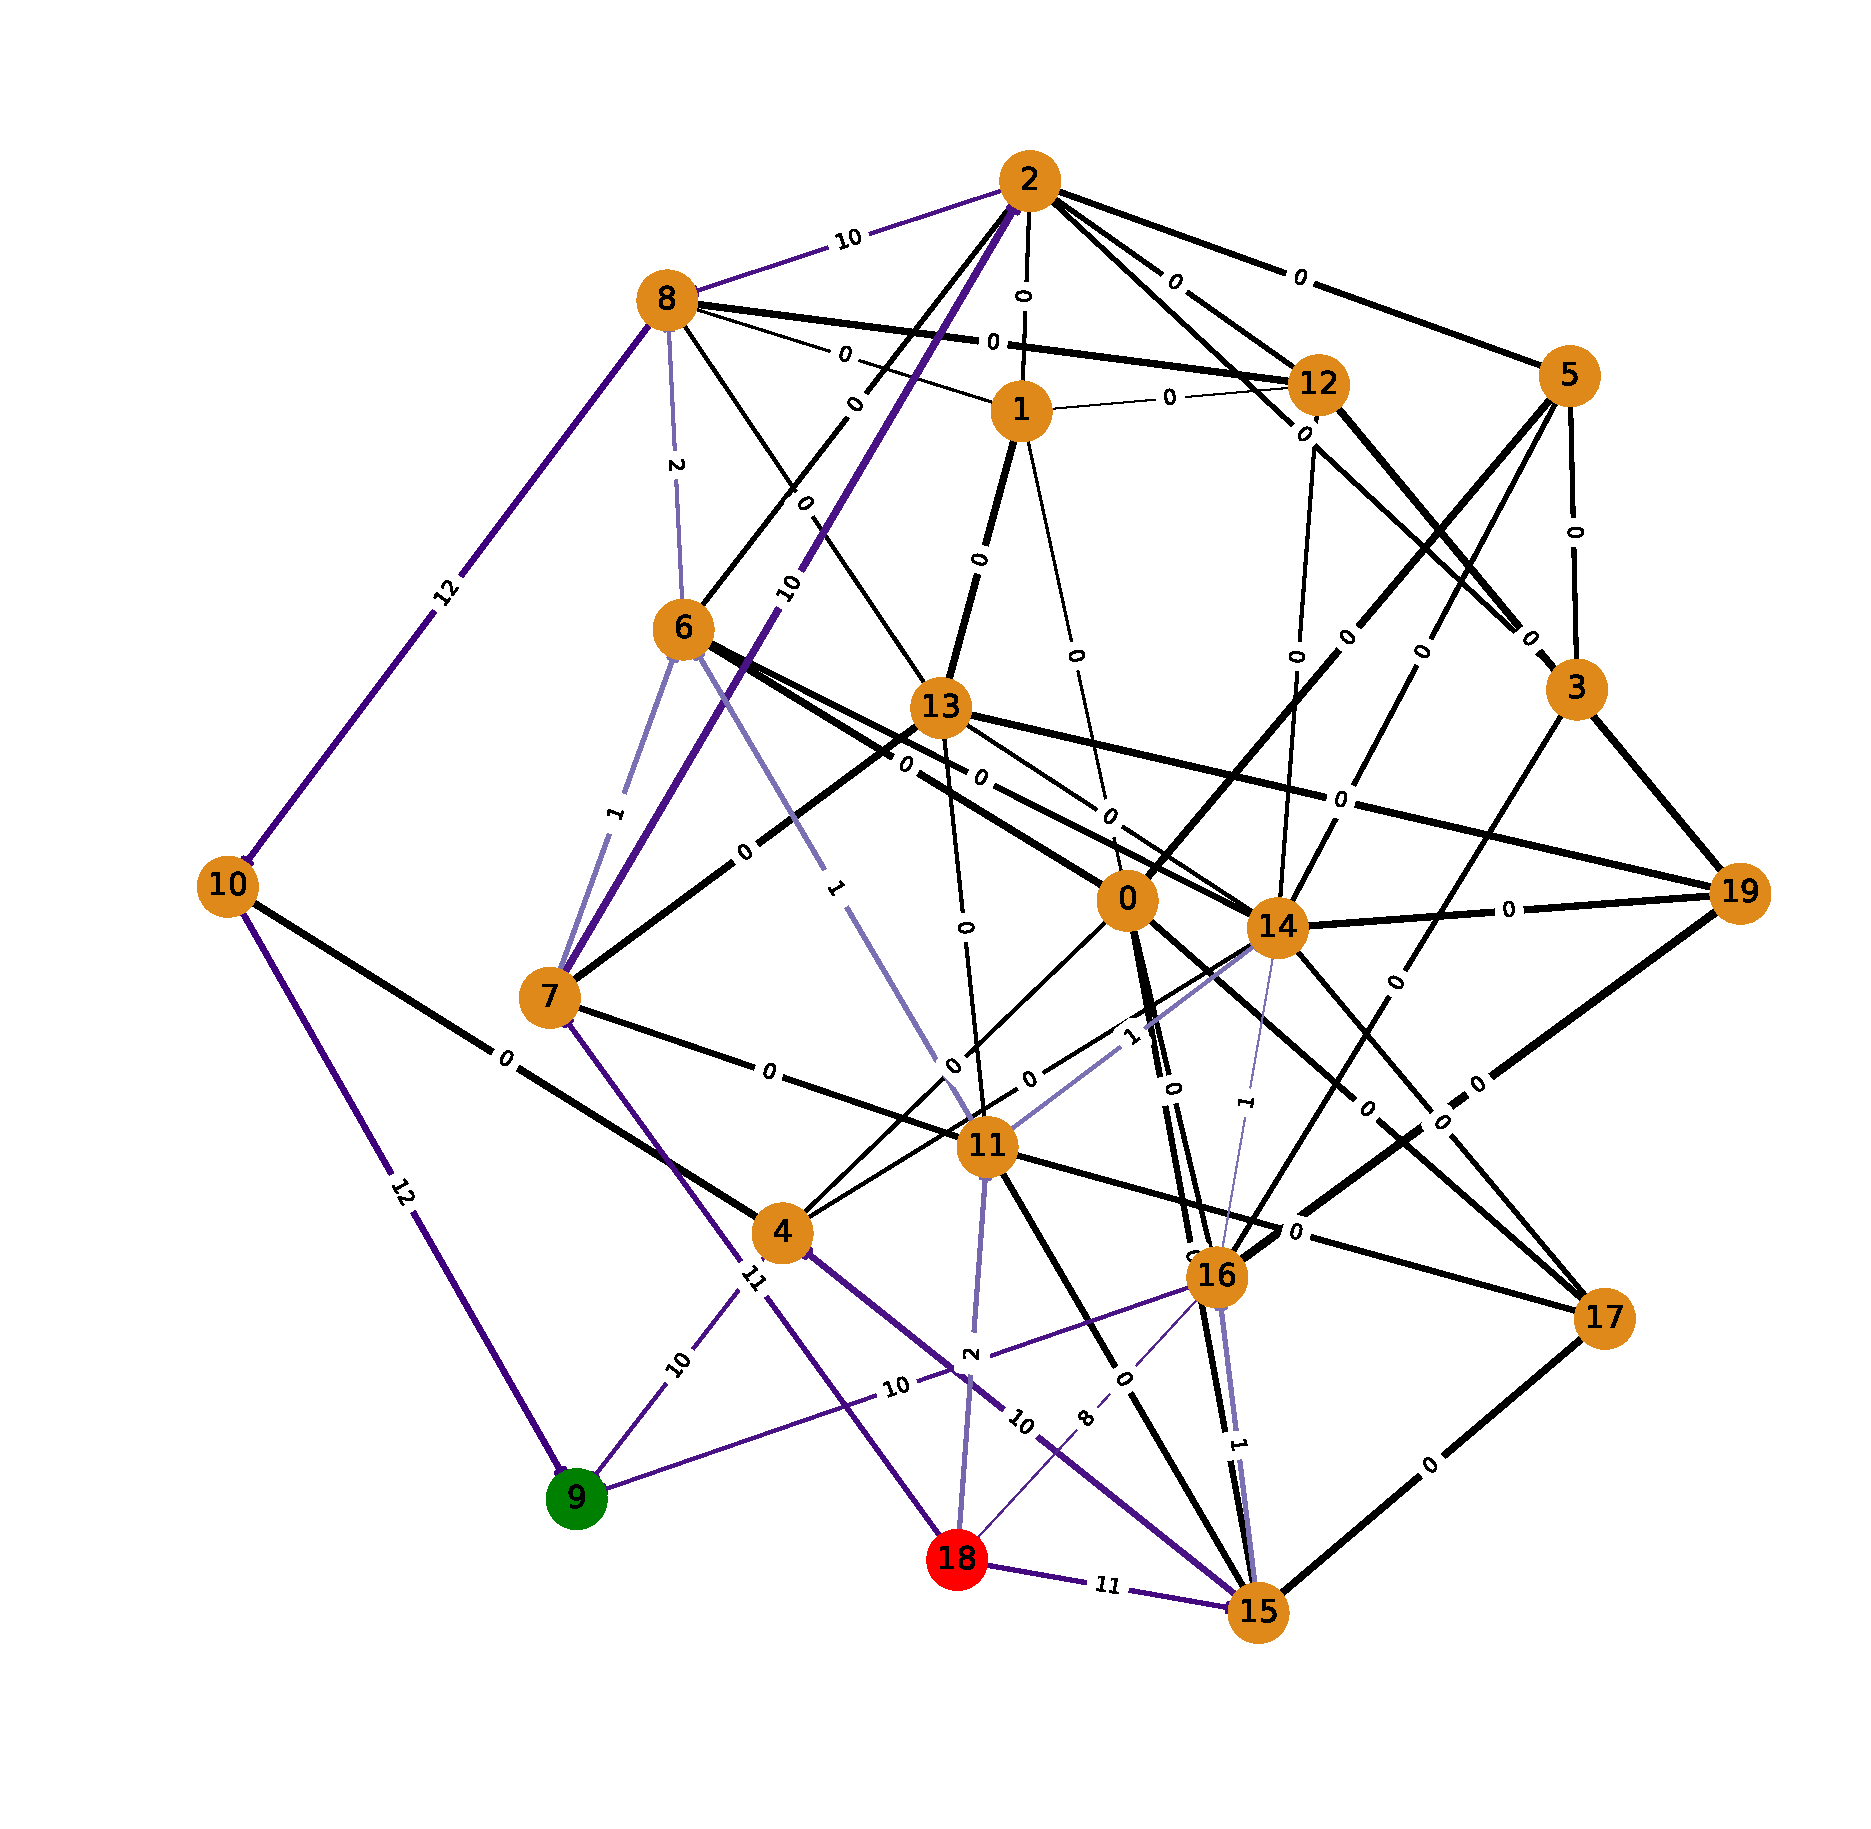
\includegraphics[scale=0.22]{Grafo4mf.eps}}
\subfigure[\textit{Grafo4}, flujo máximo 53]{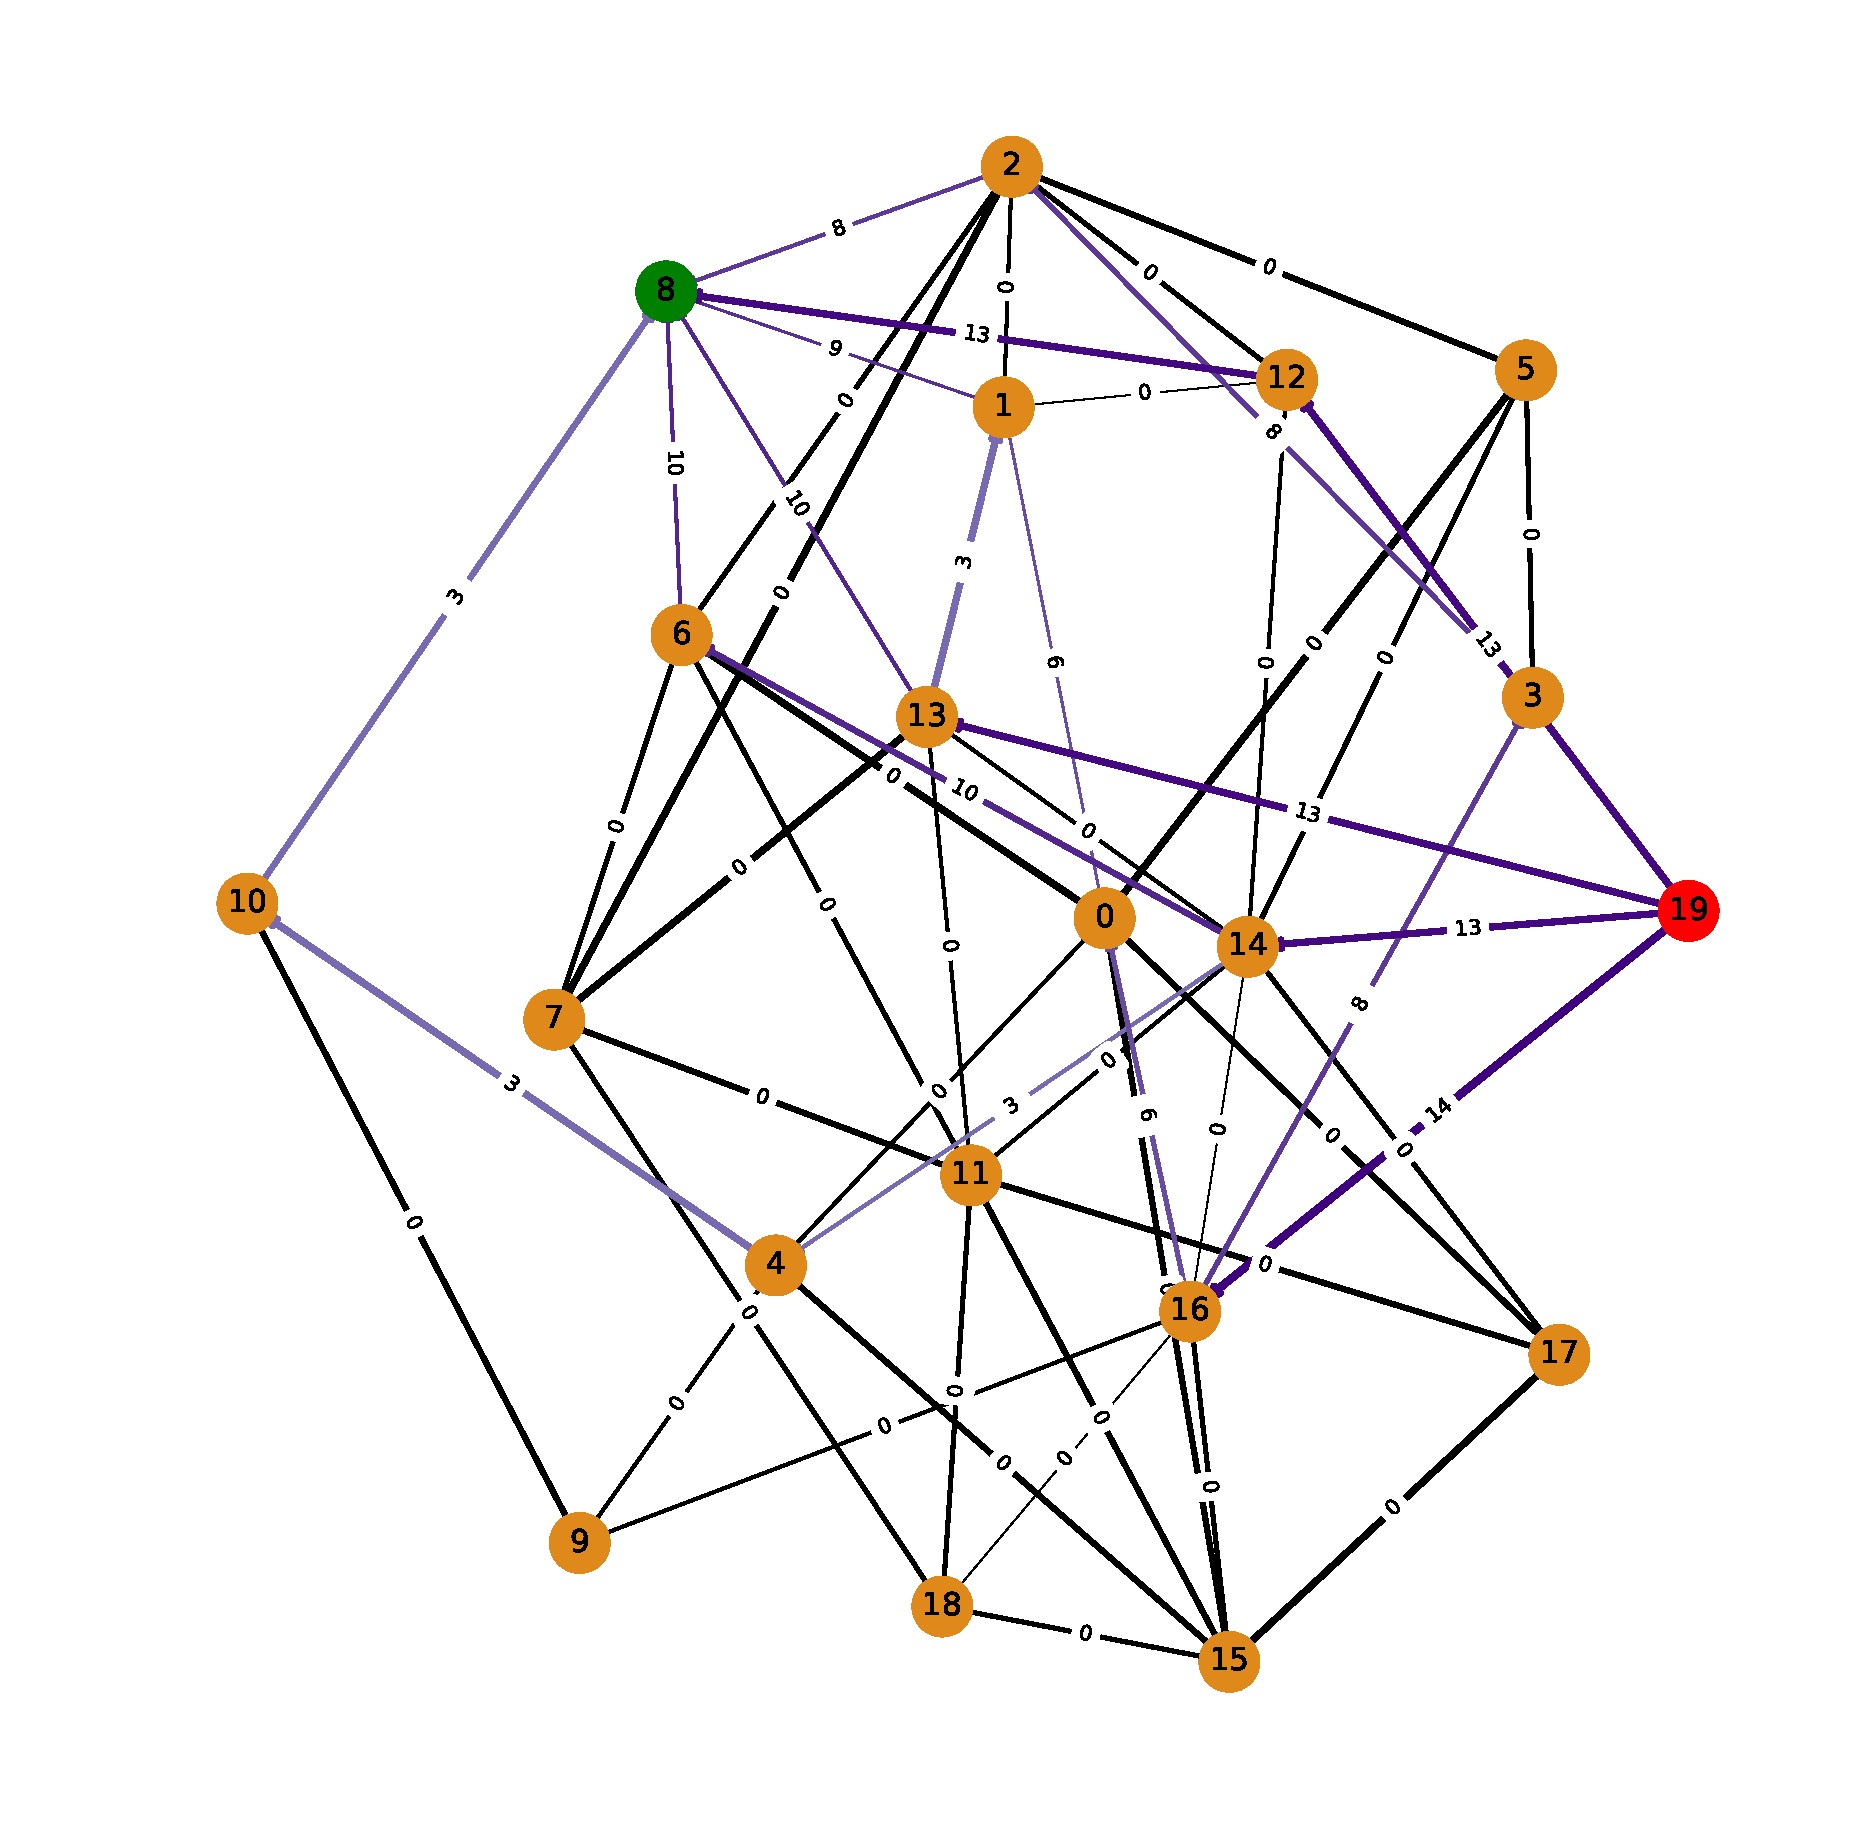
\includegraphics[scale=0.22]{Grafo4cf.eps}}
\subfigure[\textit{Grafo4}, flujo máximo 78]{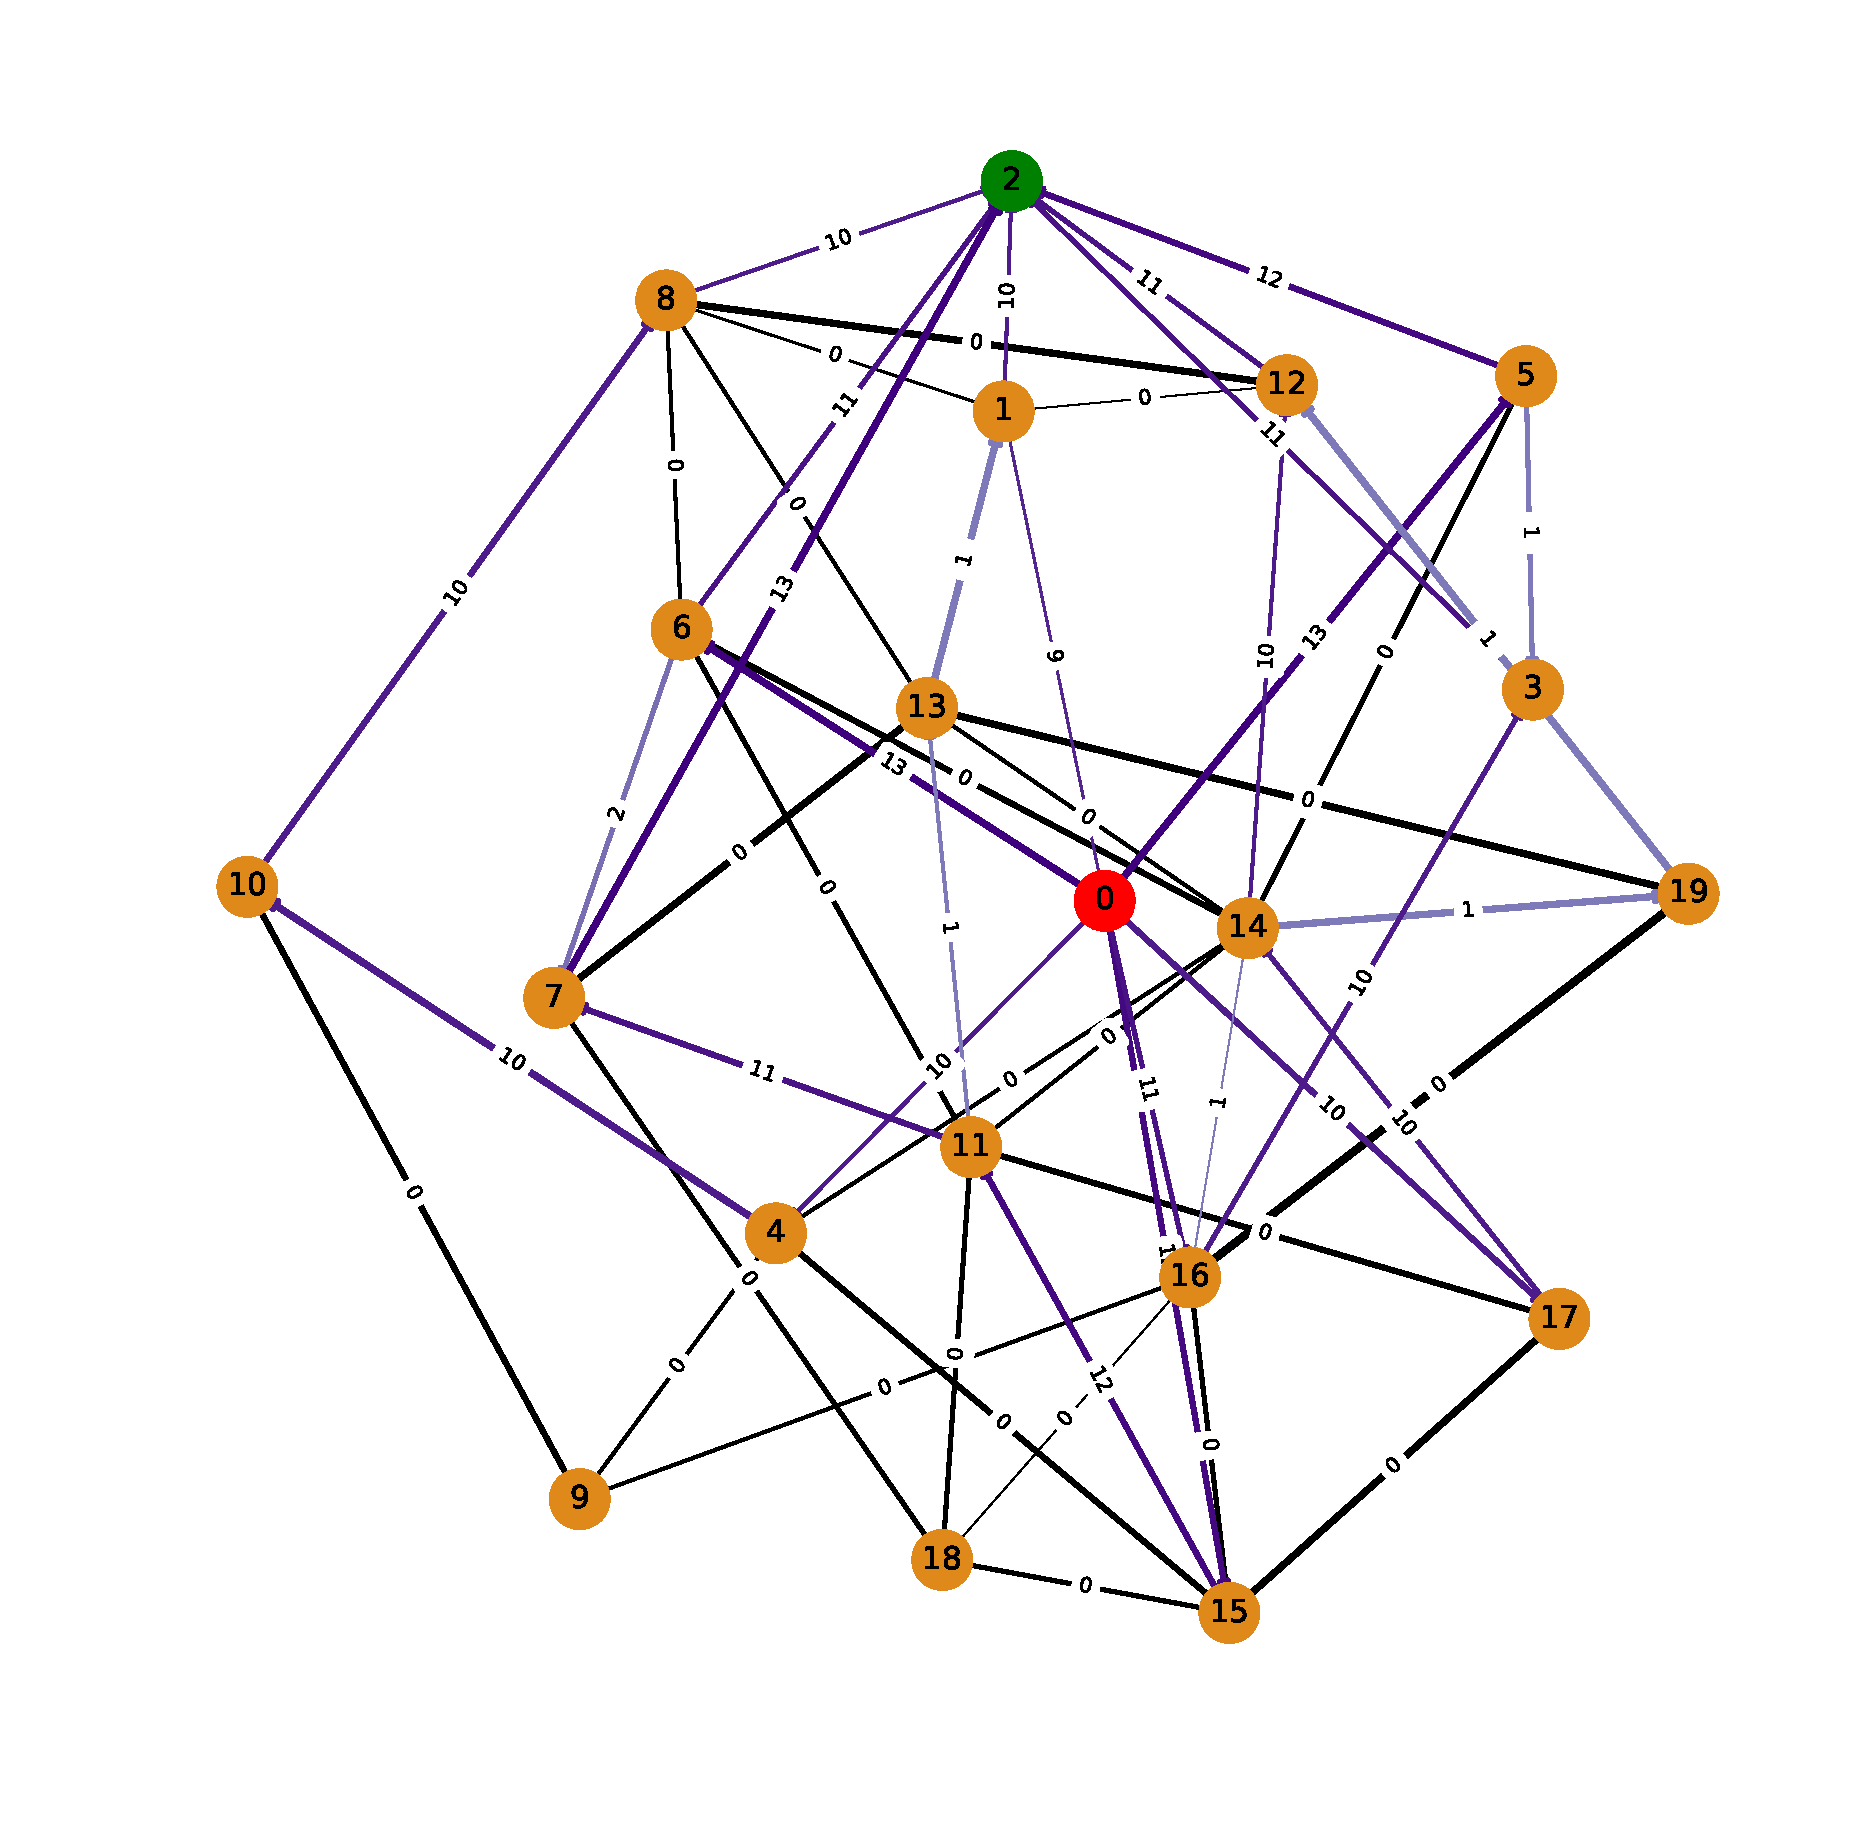
\includegraphics[scale=0.22]{Grafo4bf.eps}}
\subfigure[\textit{Grafo4}, flujo máximo 80]{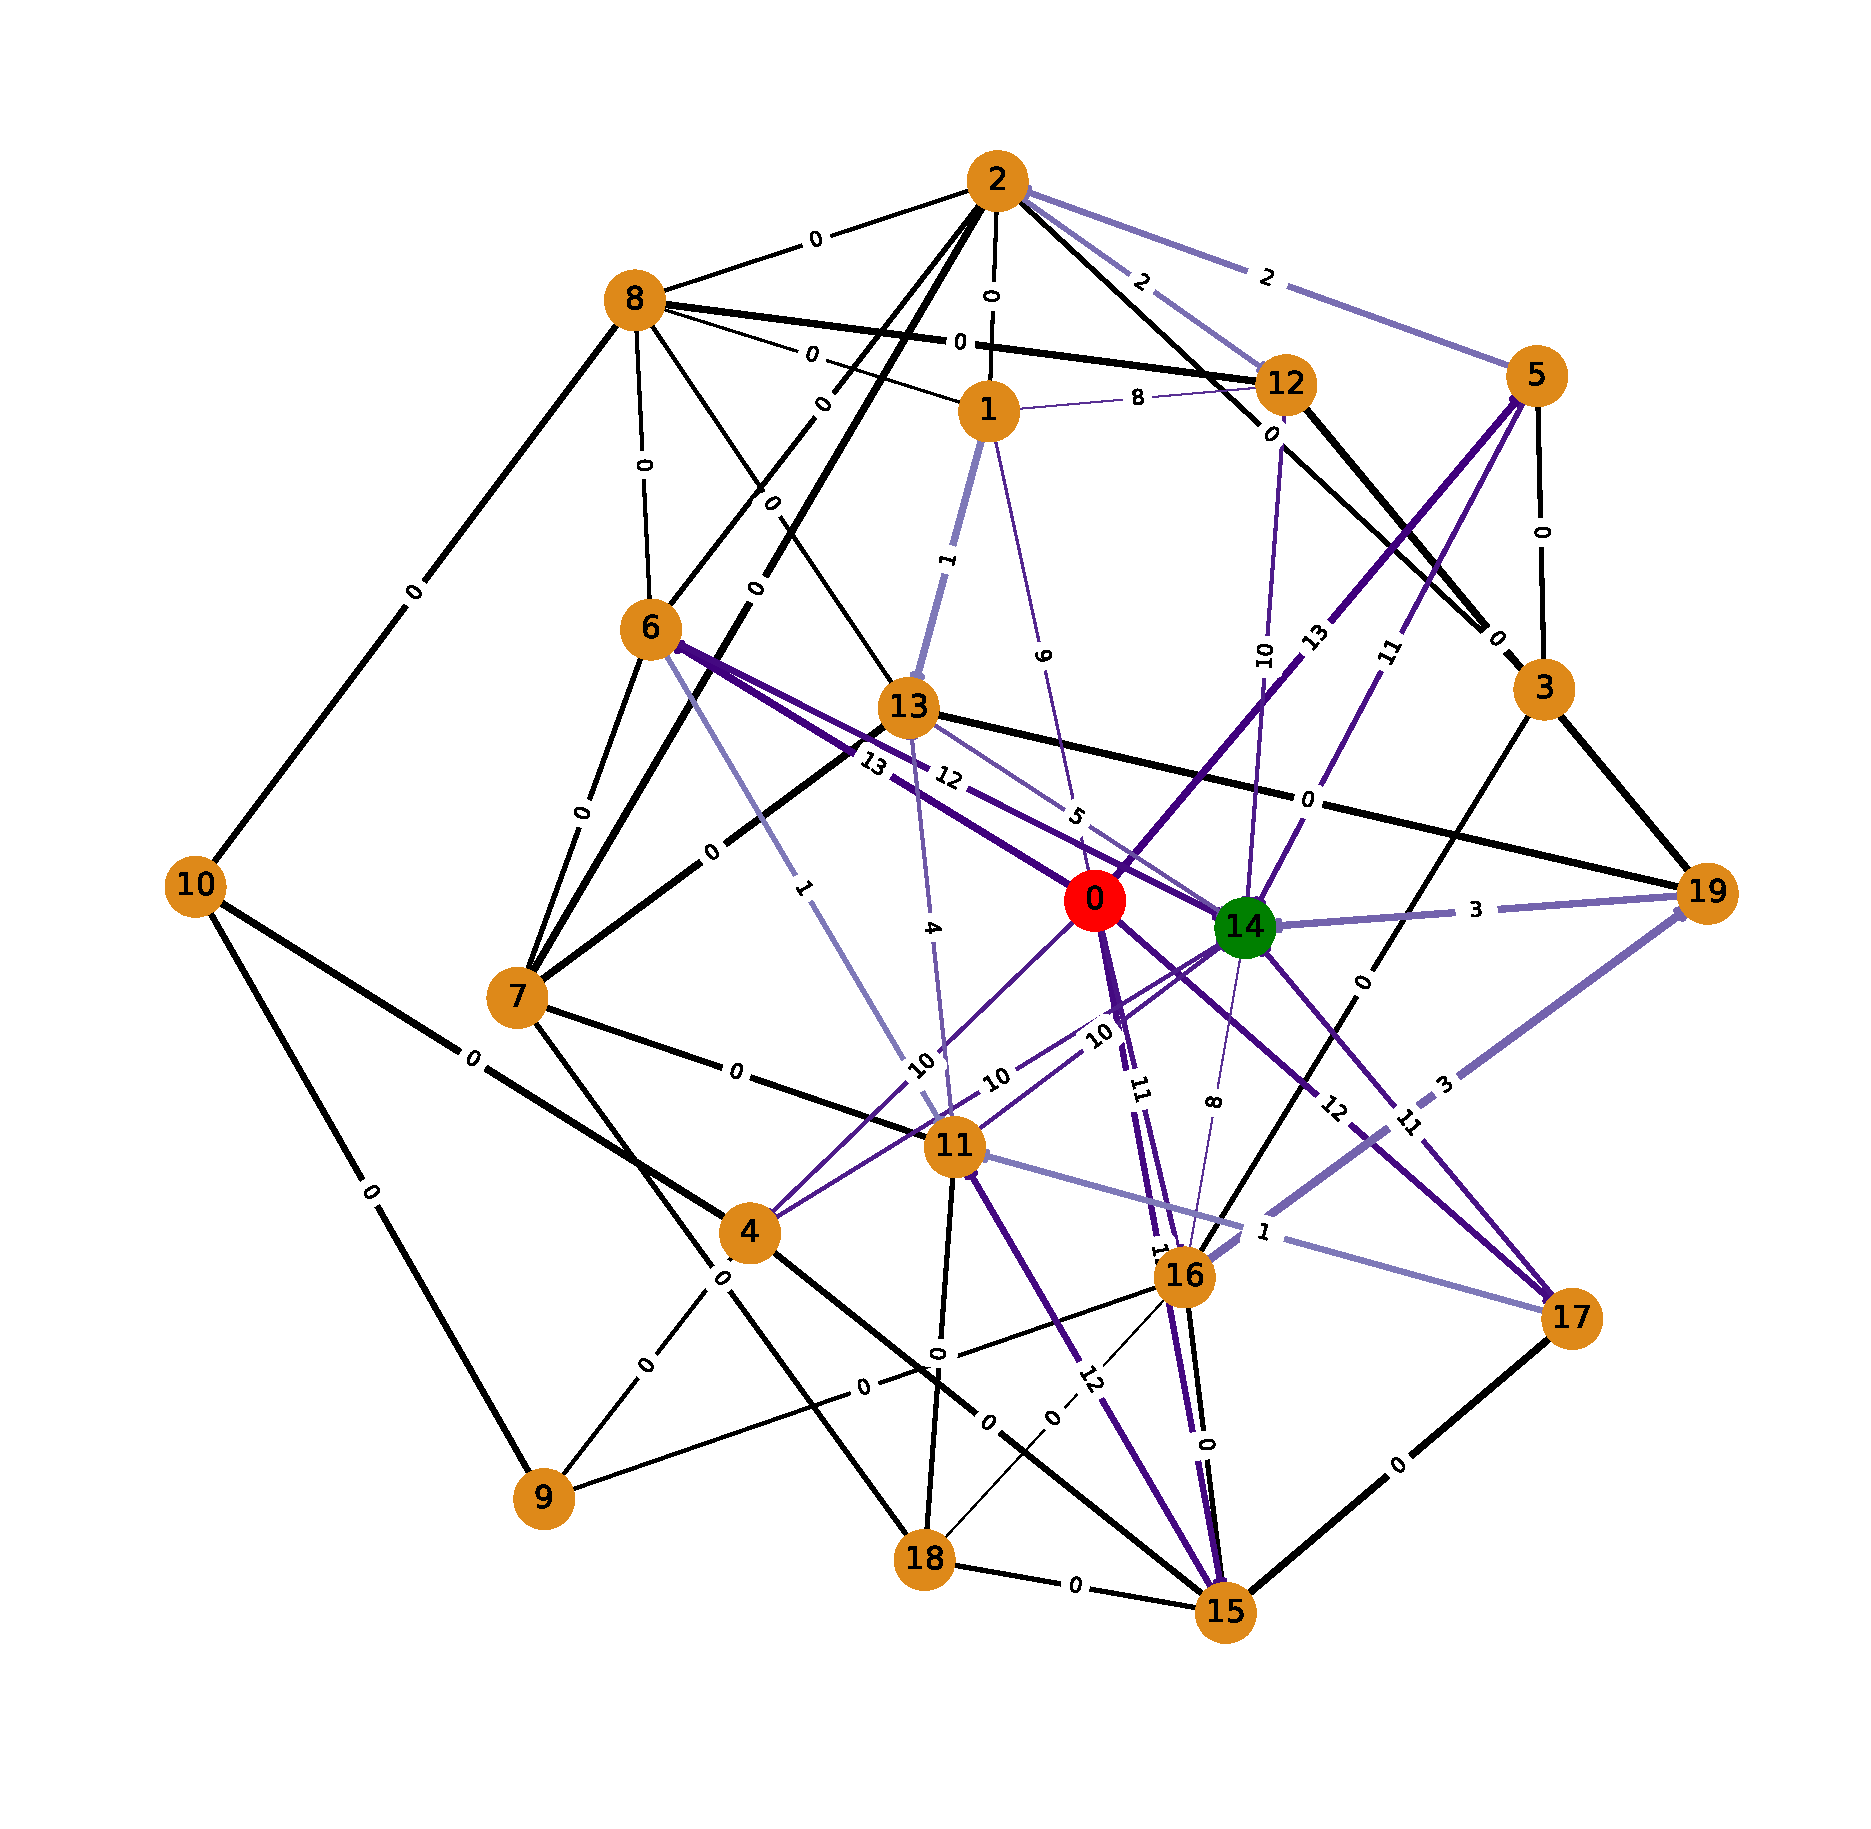
\includegraphics[scale=0.32]{Grafo4af.eps}}

\caption{Grafos resultantes de la aplicación del algoritmo de flujo máximo, donde el grosor de las aristas representa la capacidad de las mismas, el color negro la ausencia de flujo, el color violeta la presencia de flujo y la intensidad del color violeta la cantidad de flujo que pasa por la arista. El color rojo del vértice representa la fuente y el vértice verde el sumidero. }
\label{fig5} 
\end{figure}

Para el Grafo5 esto se muestra en la figura \ref{fig6} de la página \pageref{fig6}.

\begin{figure}[htbp]

\subfigure[\textit{Grafo5}, flujo máximo 12]{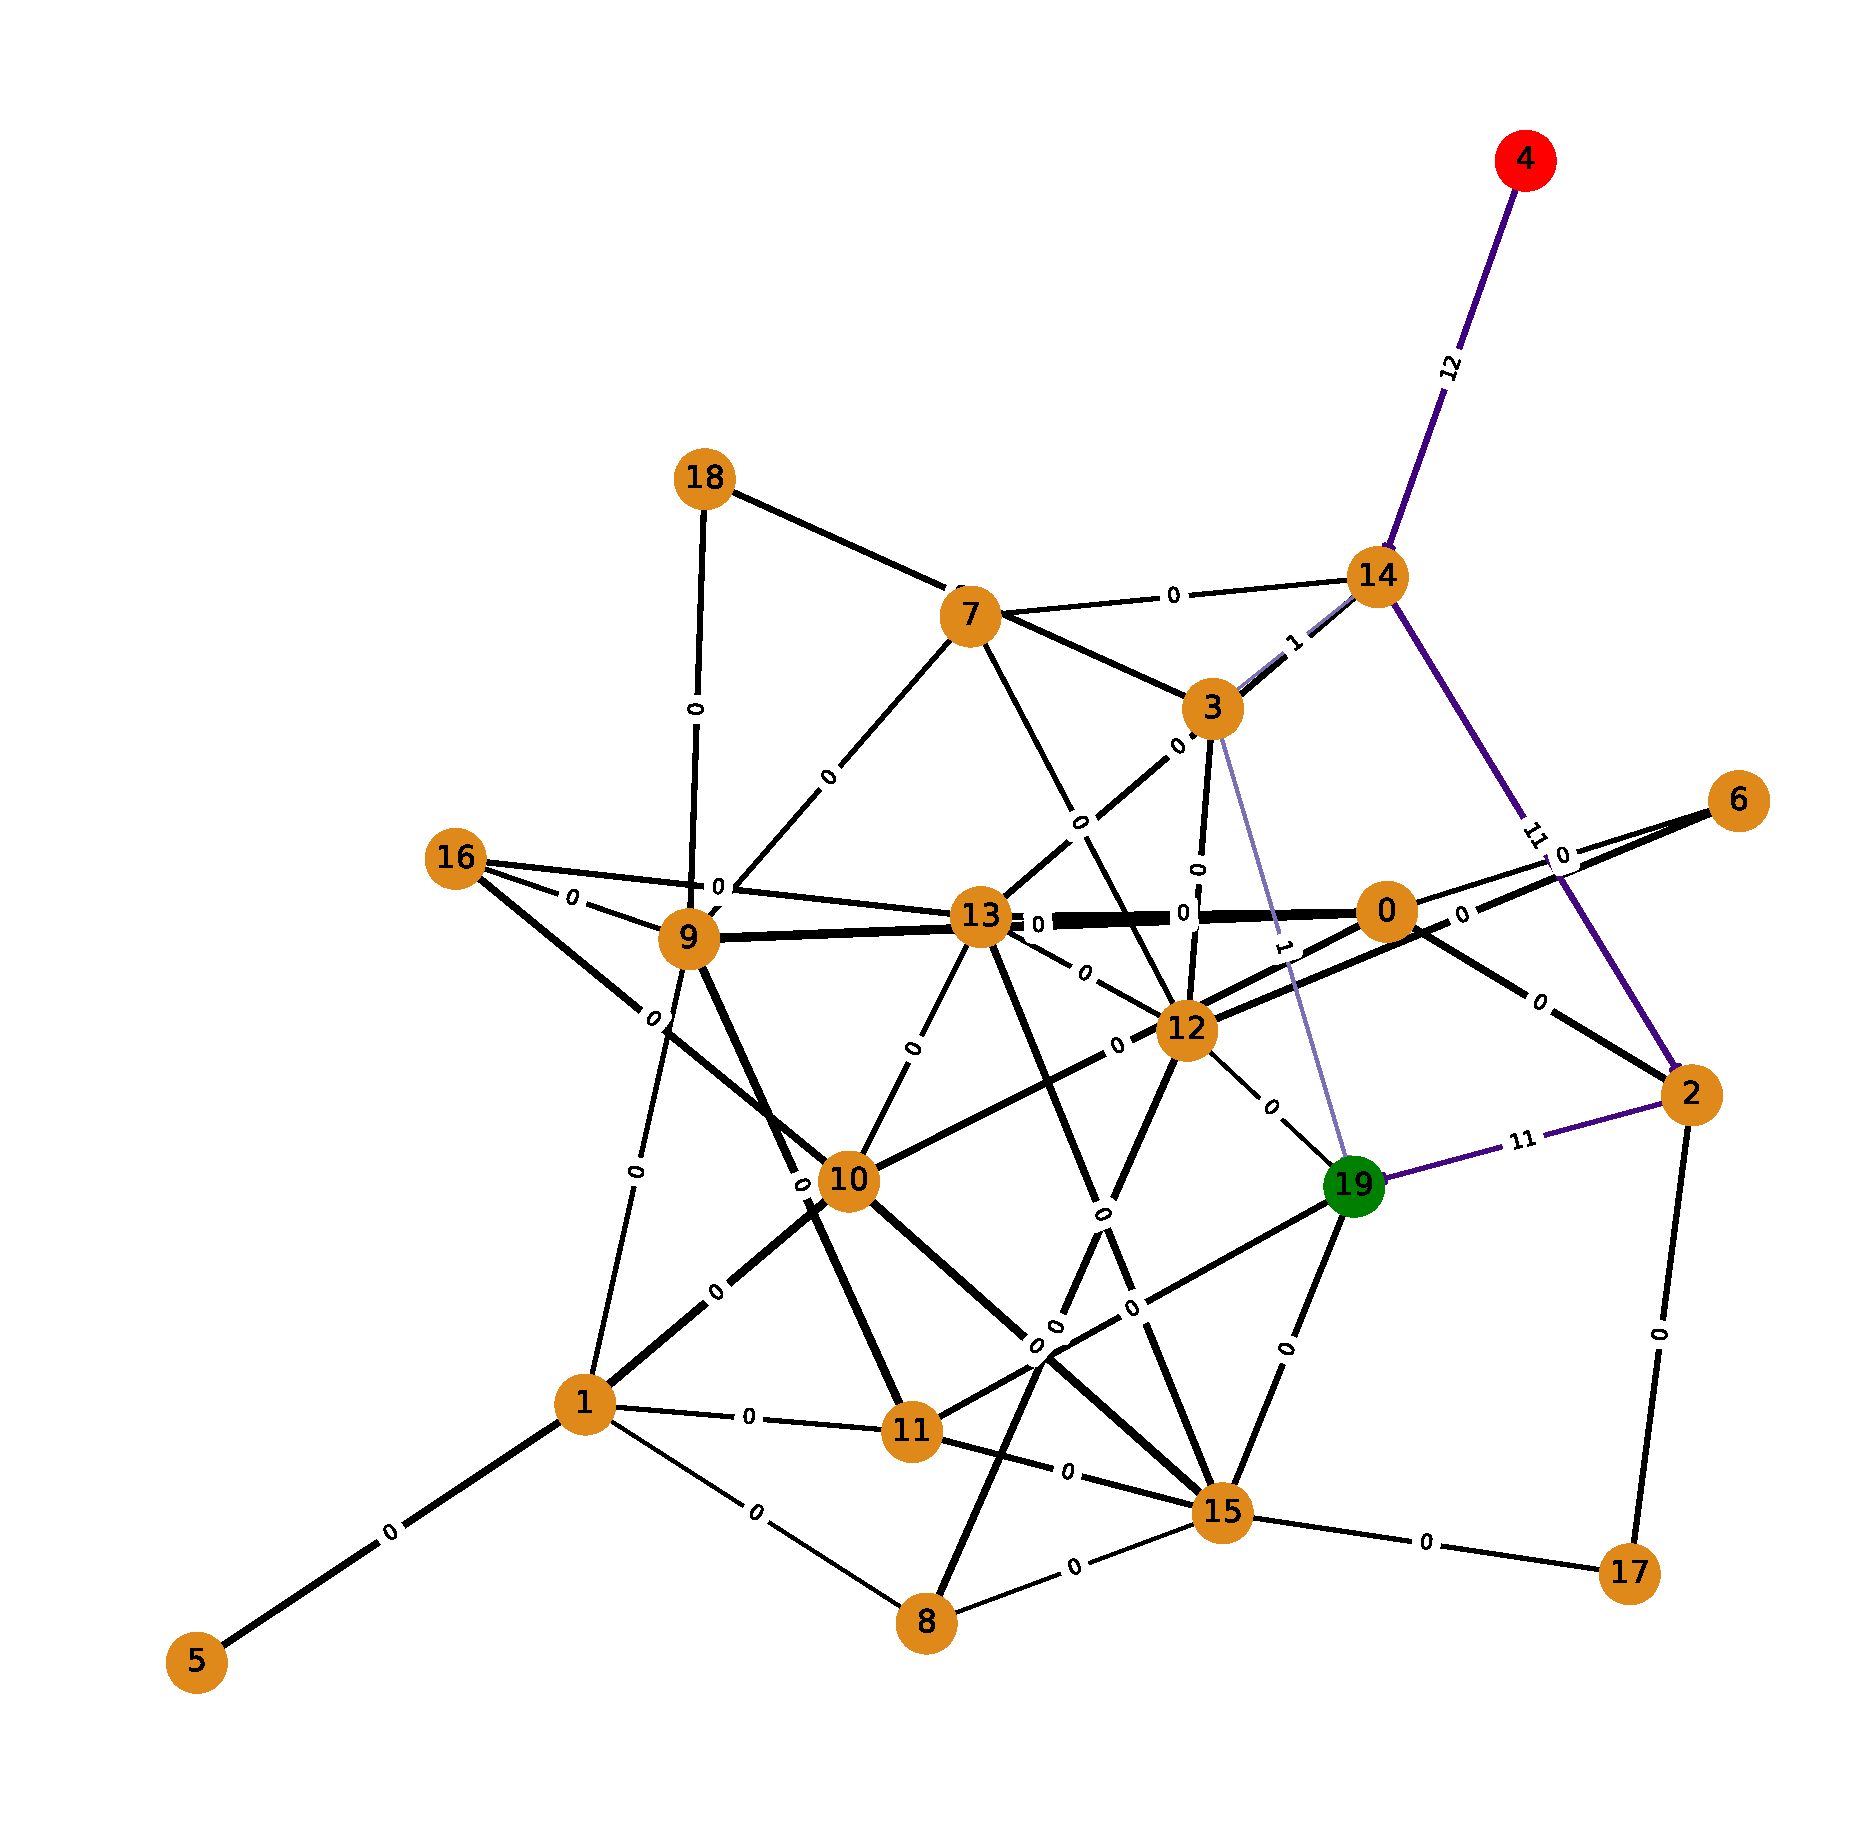
\includegraphics[scale=0.22]{Grafo5mf.eps}}
\subfigure[\textit{Grafo5}, flujo máximo 36]{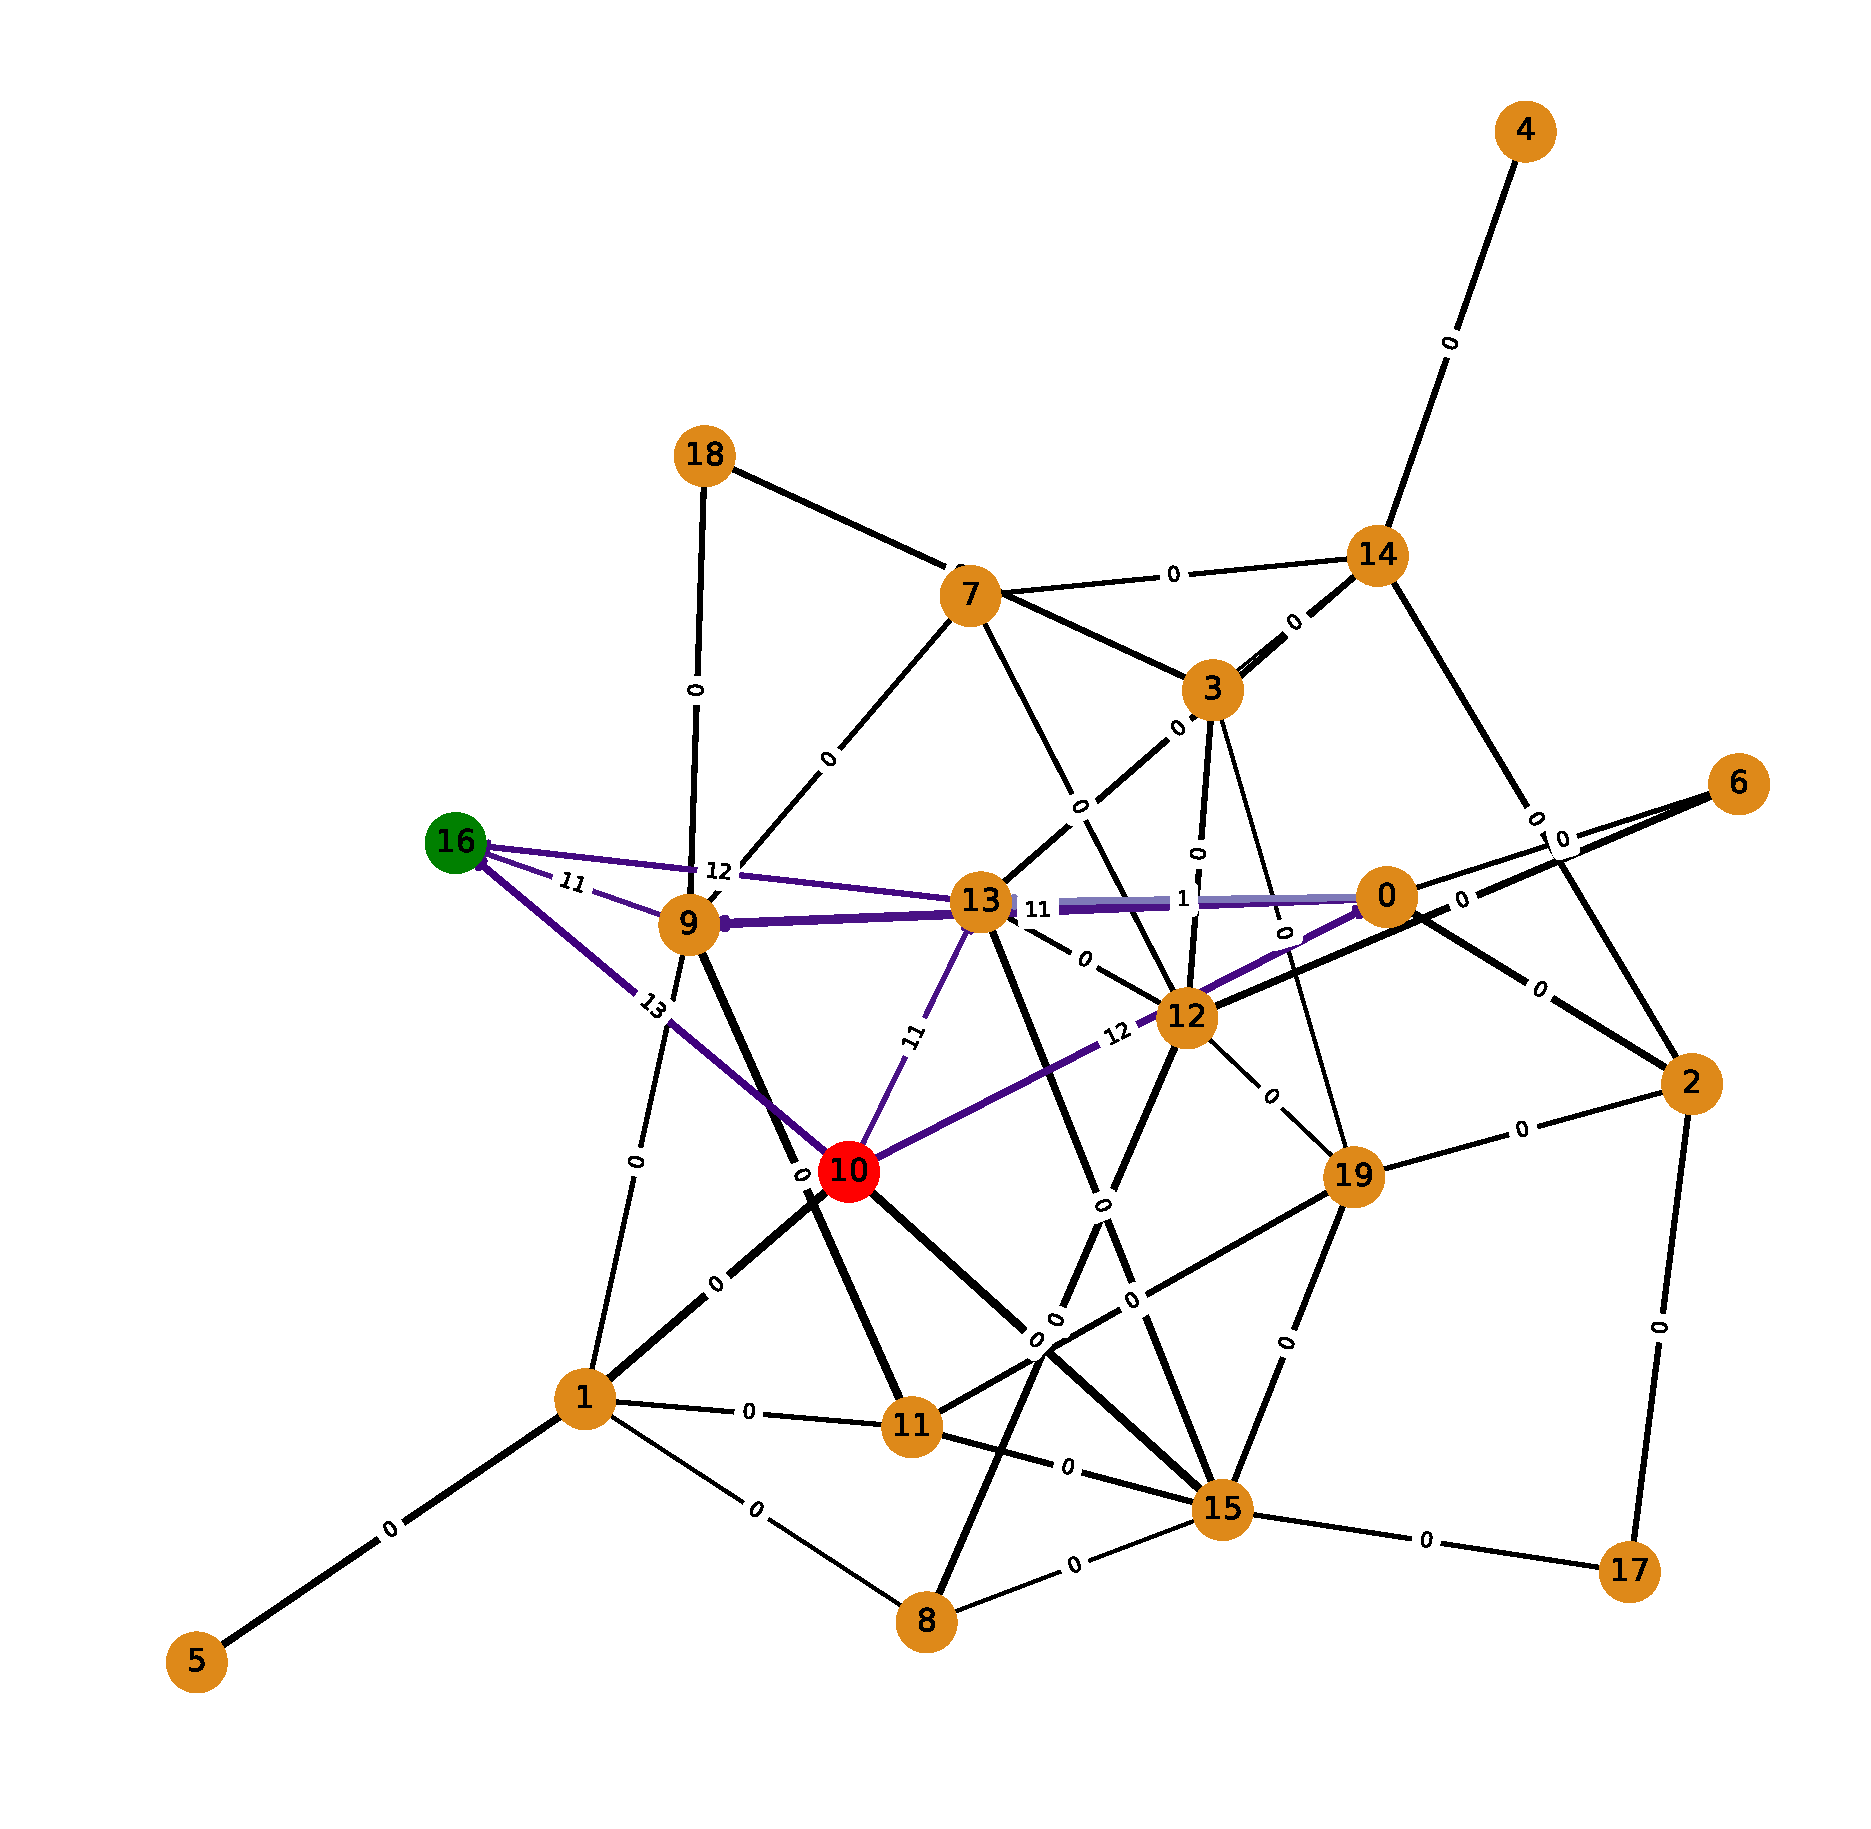
\includegraphics[scale=0.22]{Grafo5cf.eps}}
\subfigure[\textit{Grafo5}, flujo máximo 72]{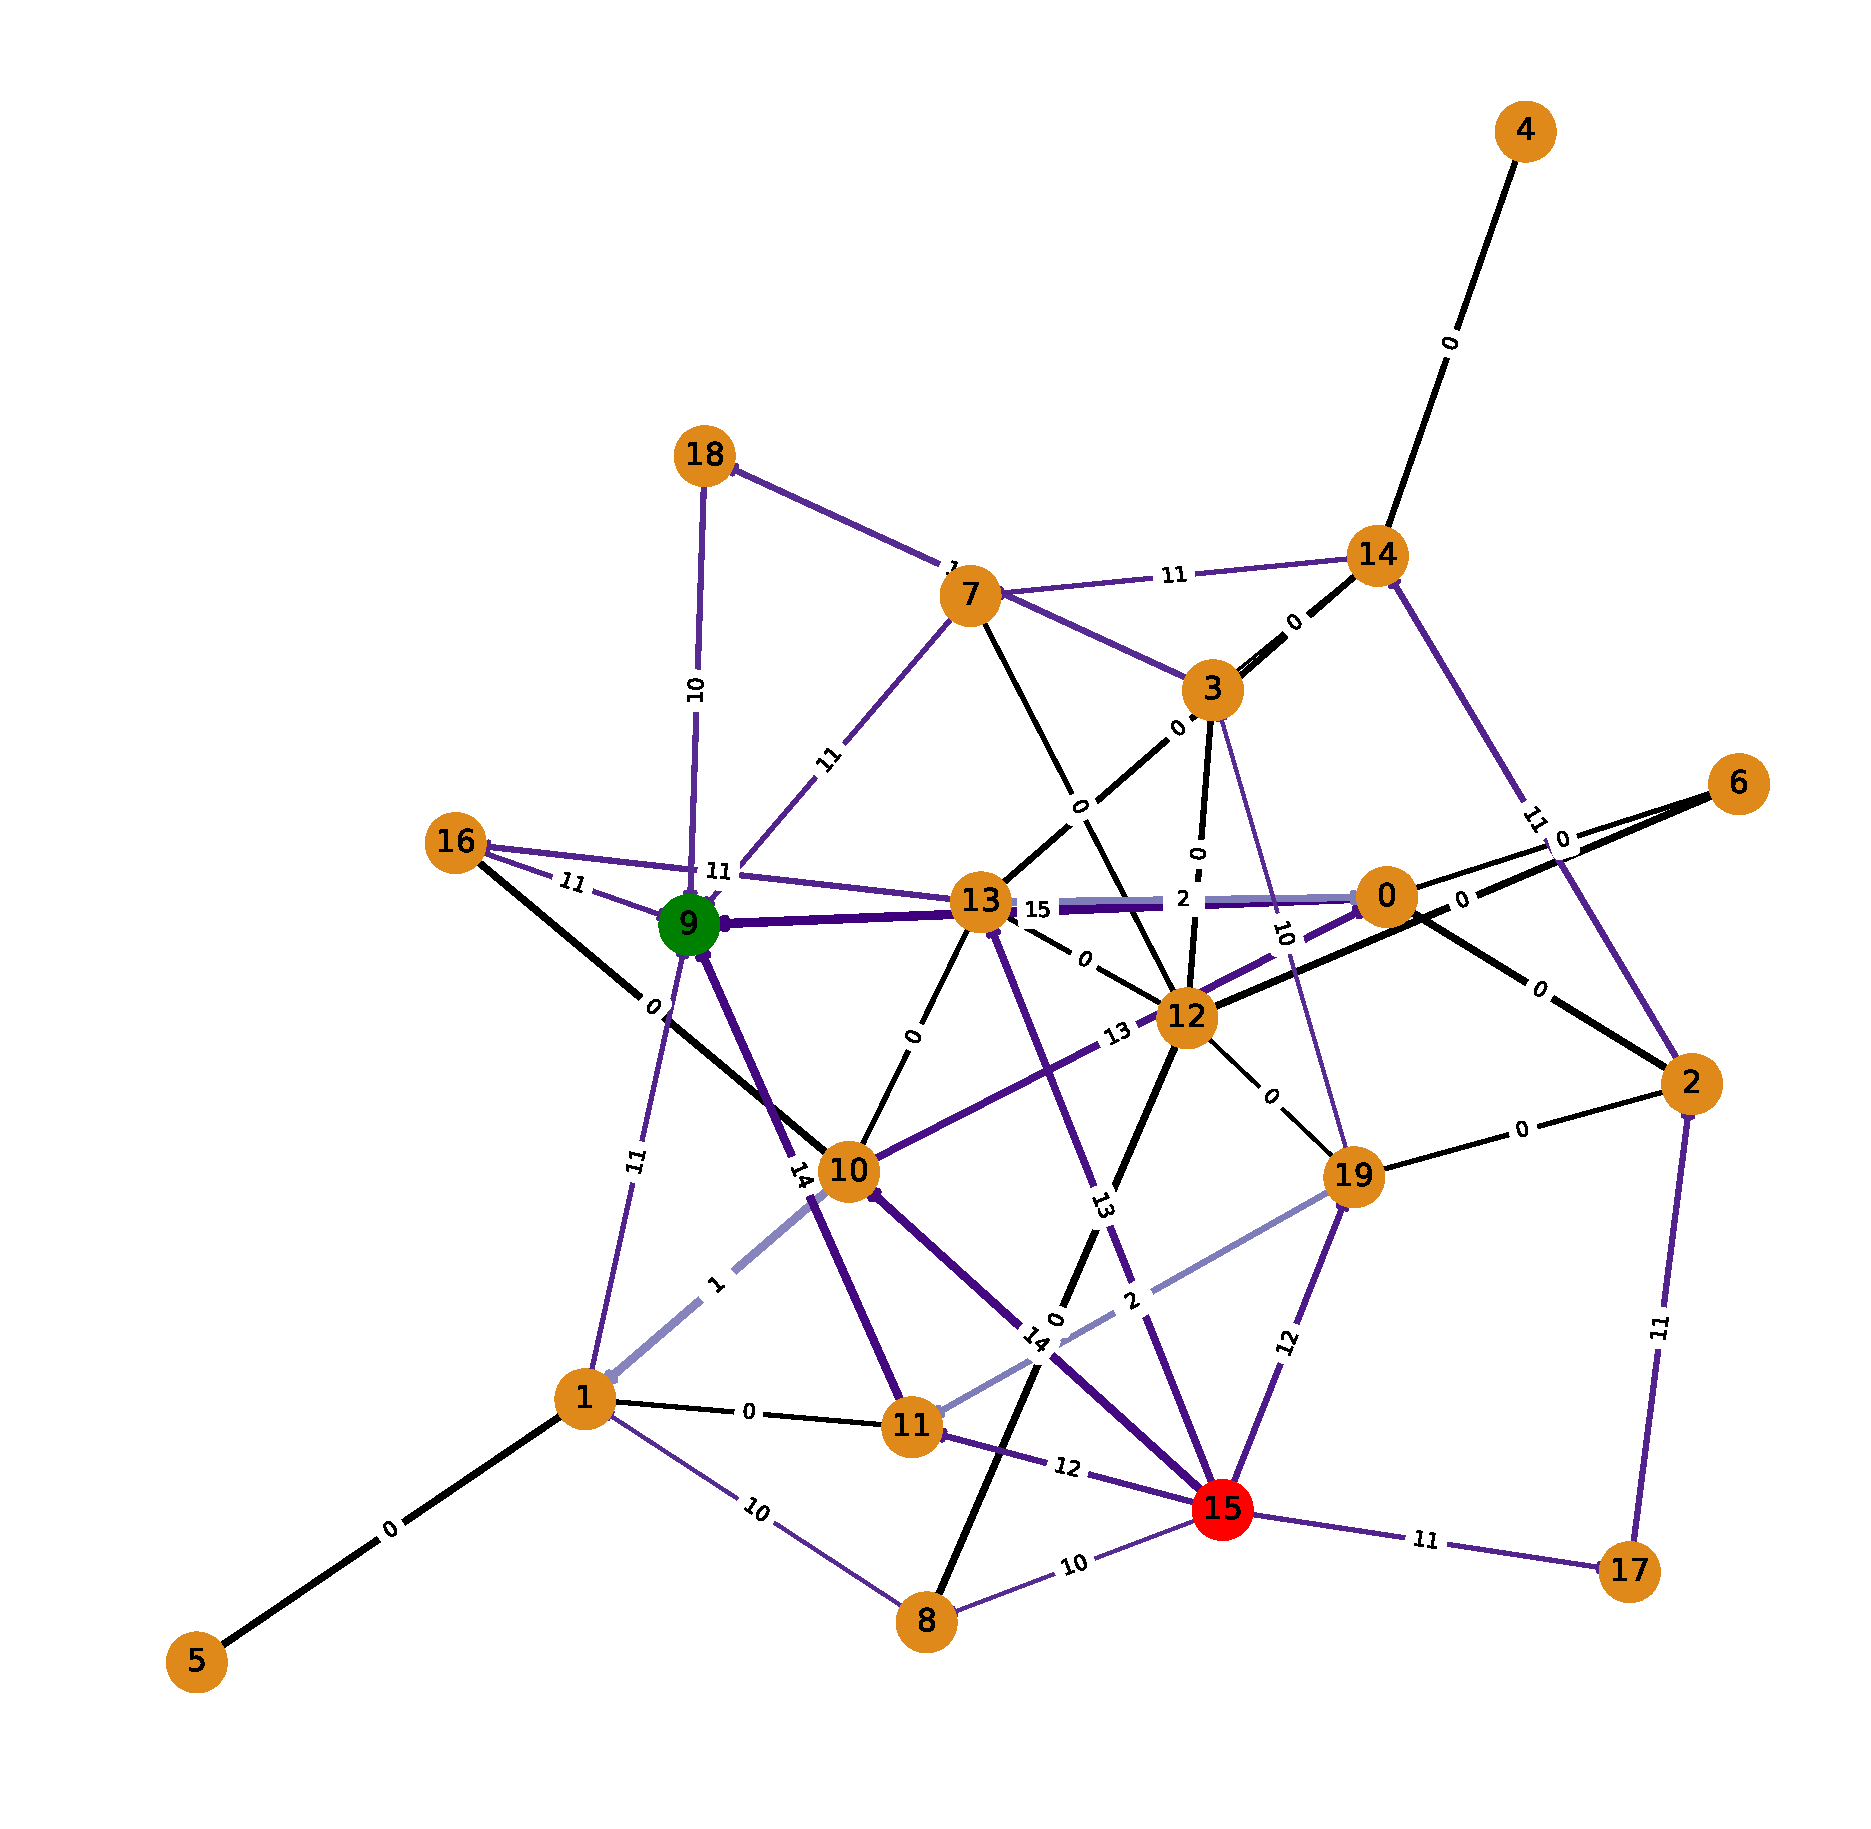
\includegraphics[scale=0.22]{Grafo5bf.eps}}
\subfigure[\textit{Grafo5}, flujo máximo 72]{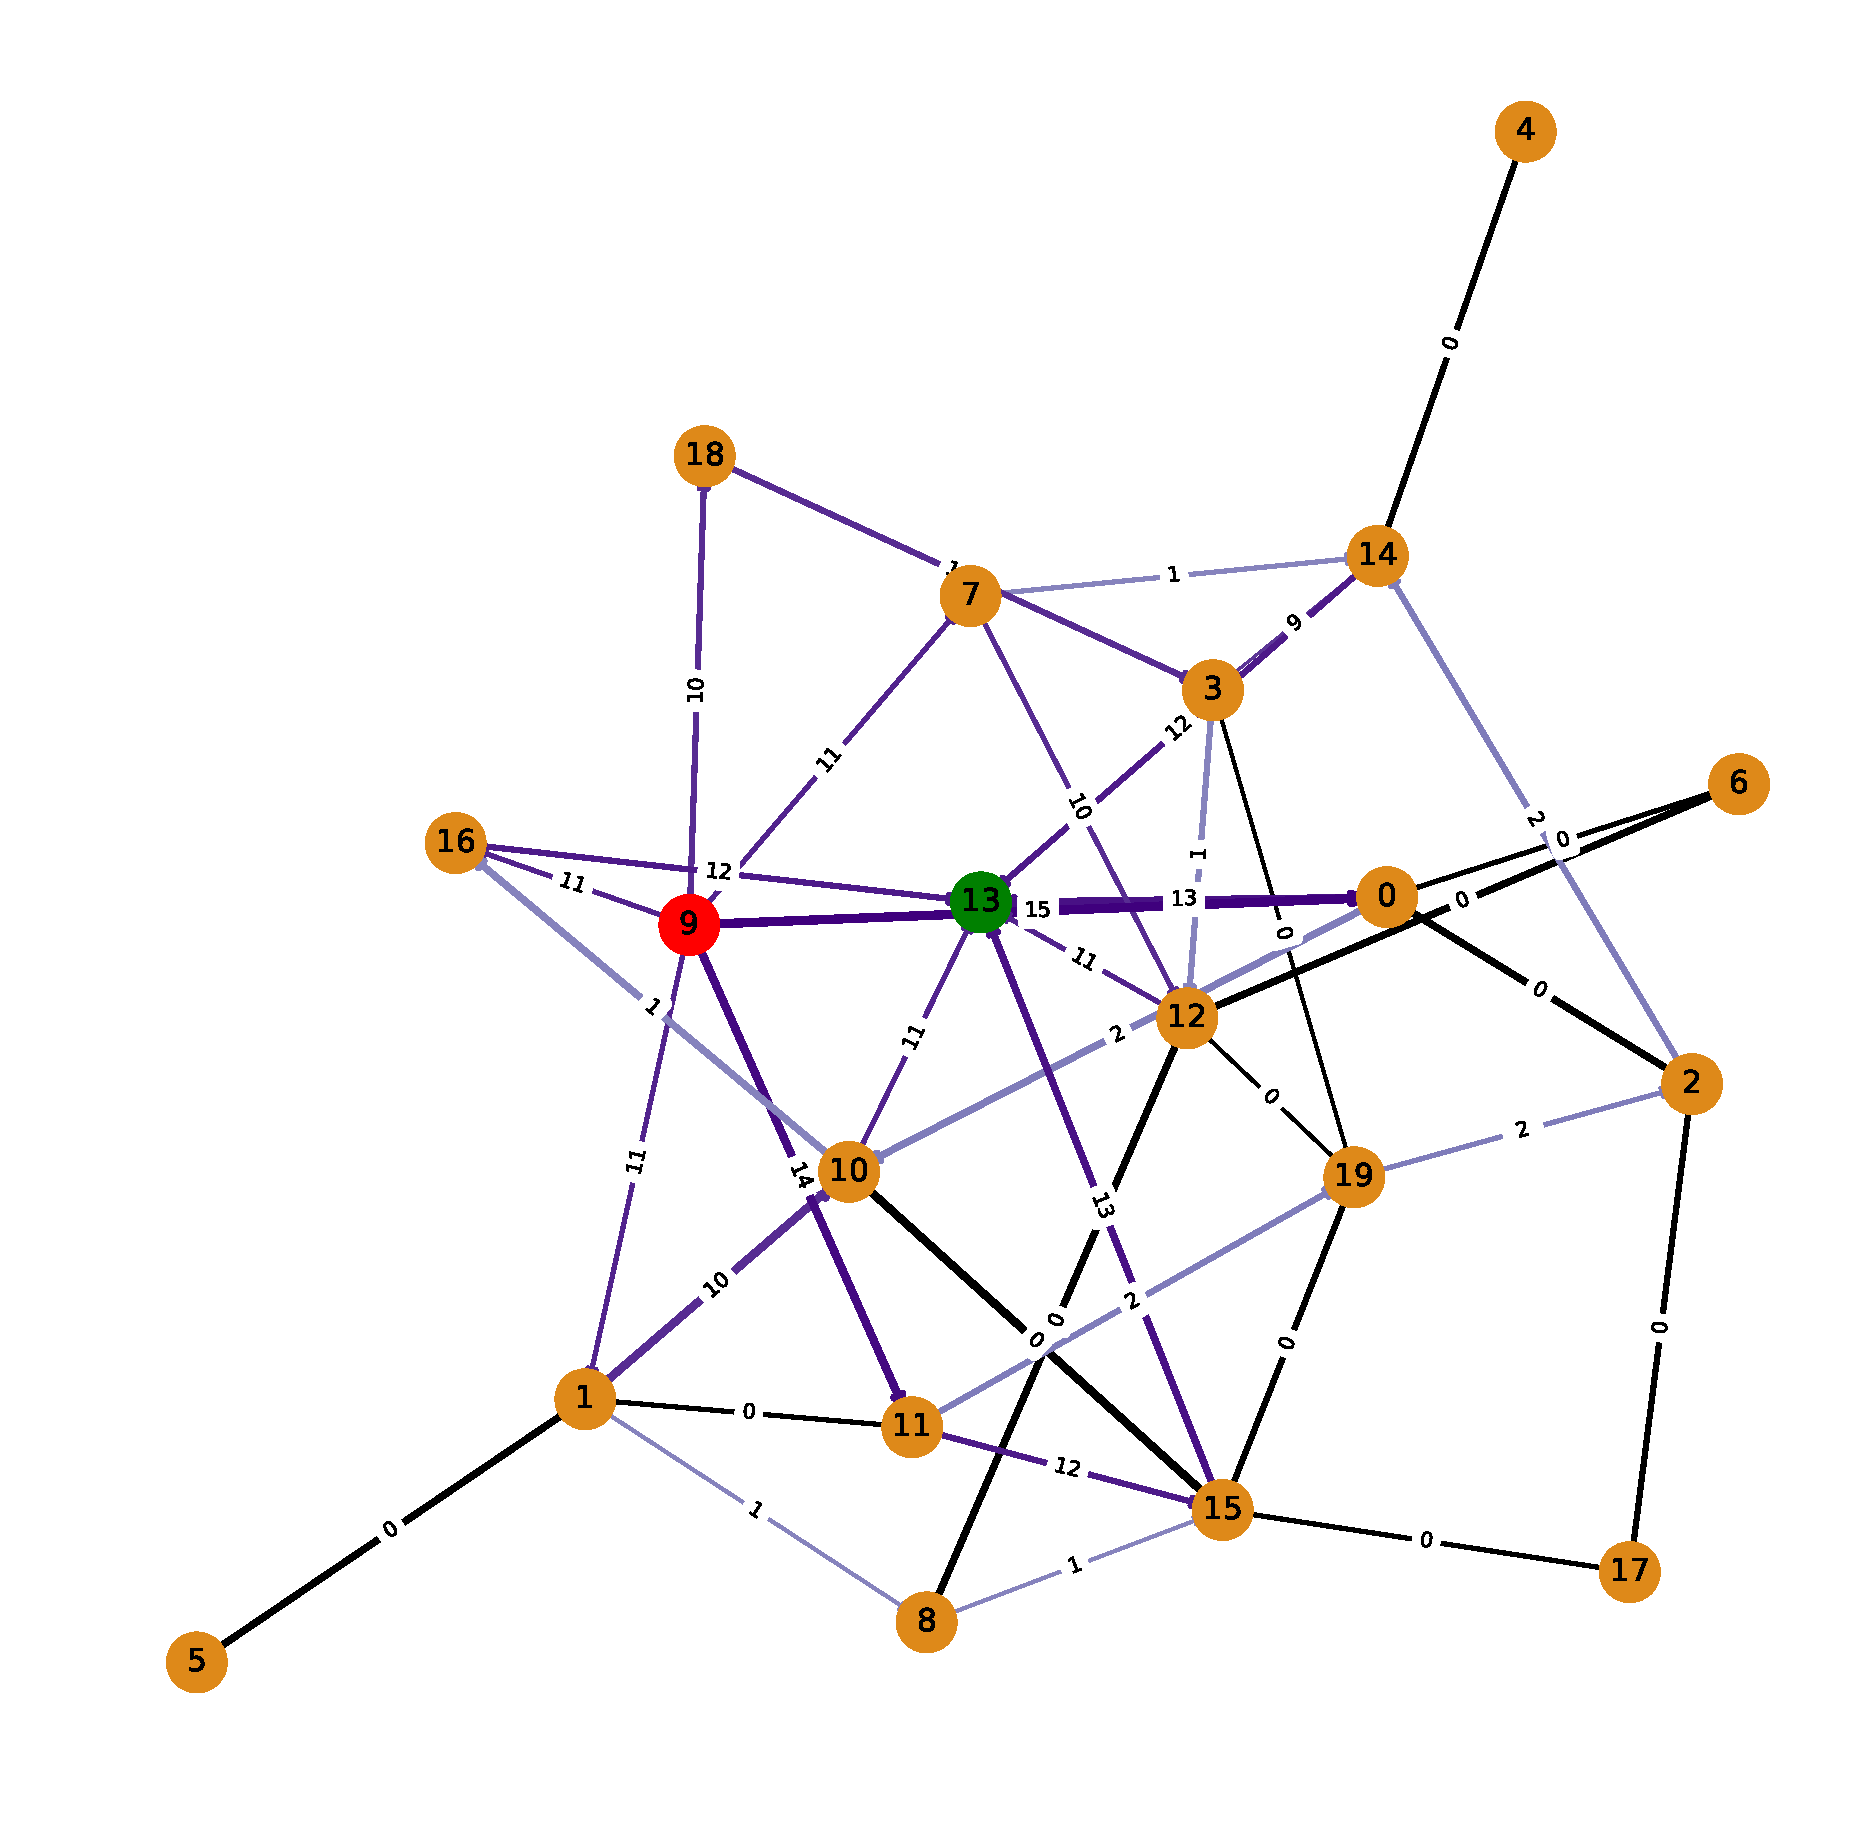
\includegraphics[scale=0.32]{Grafo5af.eps}}

\caption{Grafos resultantes de la aplicación del algoritmo de flujo máximo, donde el grosor de las aristas representa la capacidad de las mismas, el color negro la ausencia de flujo, el color violeta la presencia de flujo y la intensidad del color violeta la cantidad de flujo que pasa por la arista. El color rojo del vértice representa la fuente y el vértice verde el sumidero. }
\label{fig6} 
\end{figure}


\section{Resultados del análisis de los datos}


Con los datos recopilado de las ejecuciones del algoritmo de flujo máximo en los cinco grafos y todas las posibles combinaciones de fuentes y sumidero, se realizó histogramas para cada una de las seis características en los cinco grafos para determinar si los valores de la media del tiempo de ejecución tienen una distribución normal. Estos histogramas nos indican que la distribución no es normal como muestran la figuras \ref{fig7}, \ref{fig8}, \ref{fig9}, \ref{fig10}, \ref{fig11}, \ref{fig12} de las páginas \pageref{fig7}, \pageref{fig8}, \pageref{fig9}, \pageref{fig10}, \pageref{fig11}, \pageref{fig12} respectivamente.  

\begin{figure}[htbp]

\subfigure[\textit{Grafo1}]{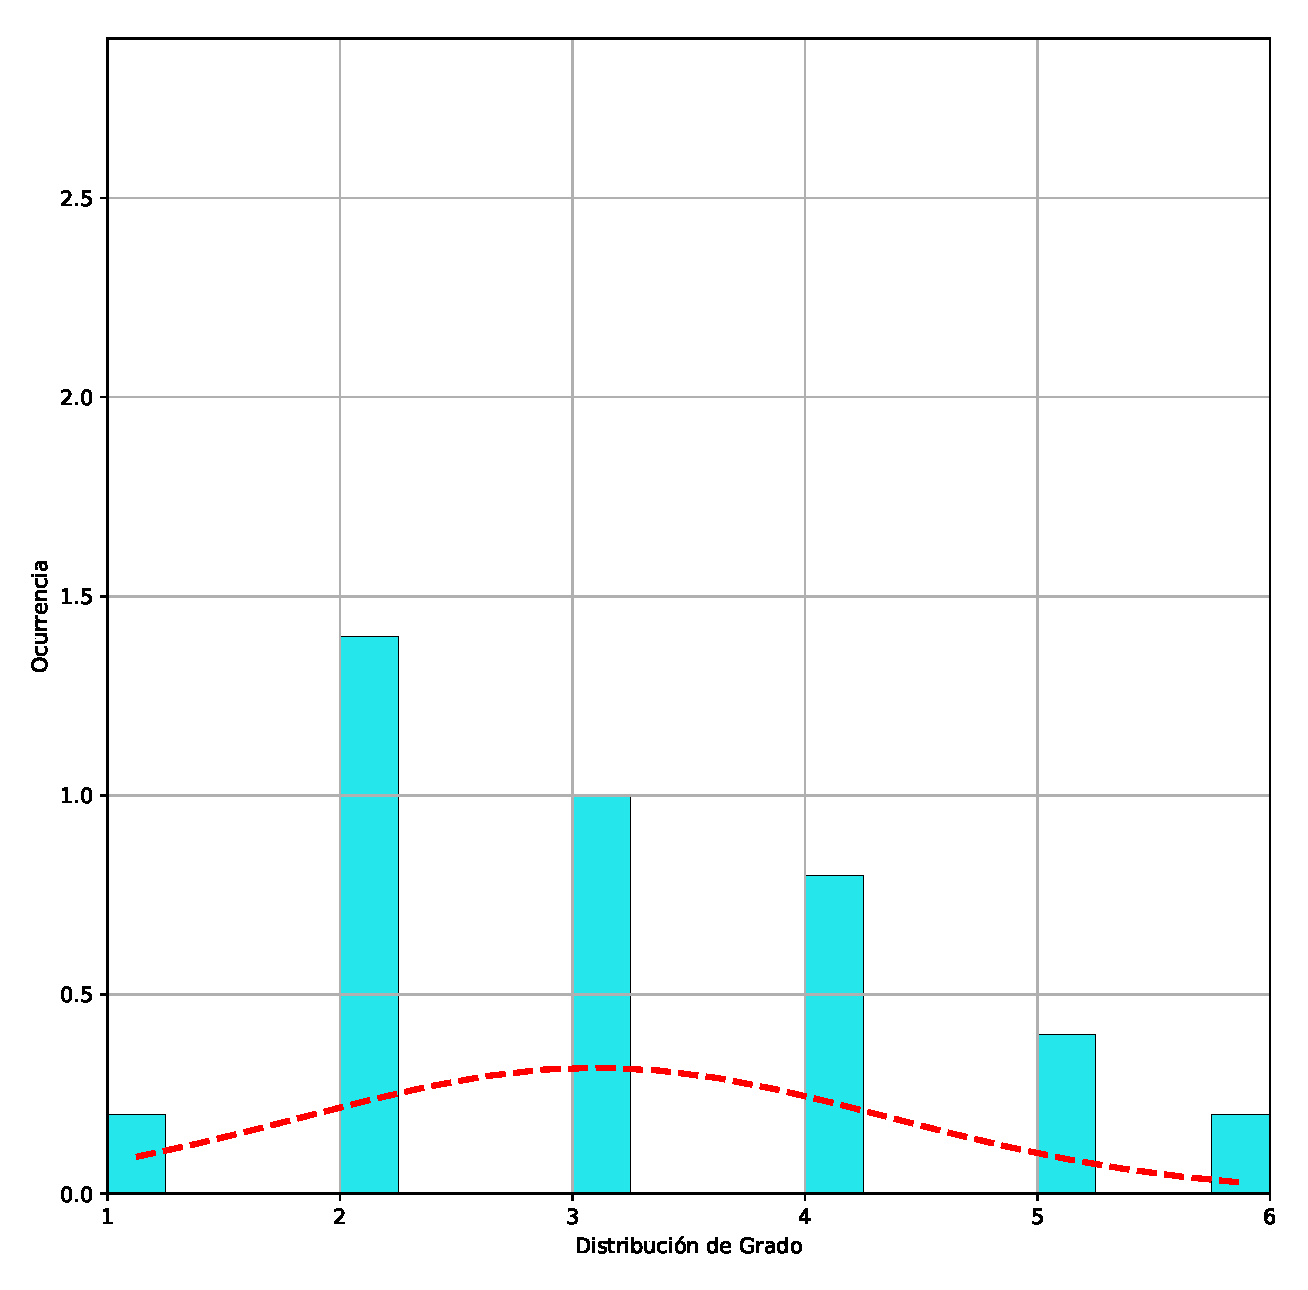
\includegraphics[scale=0.3]{GradoGrafo1D.eps}}
\subfigure[\textit{Grafo2}]{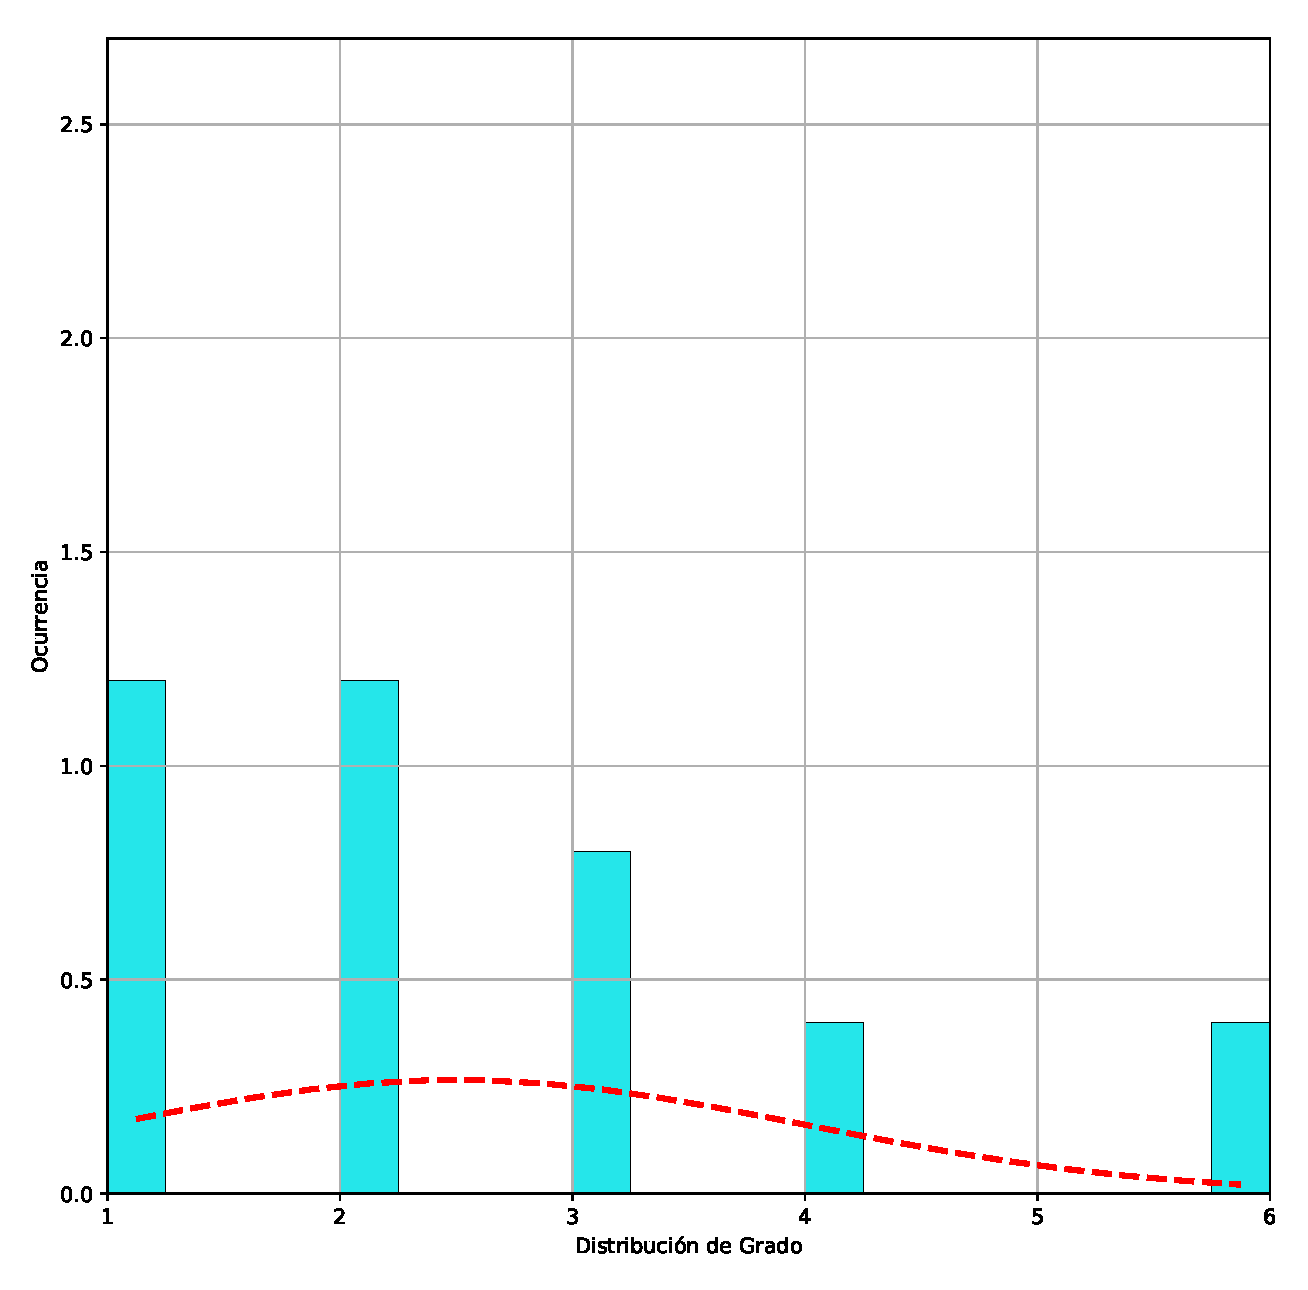
\includegraphics[scale=0.3]{GradoGrafo2D.eps}}
\subfigure[\textit{Grafo3}]{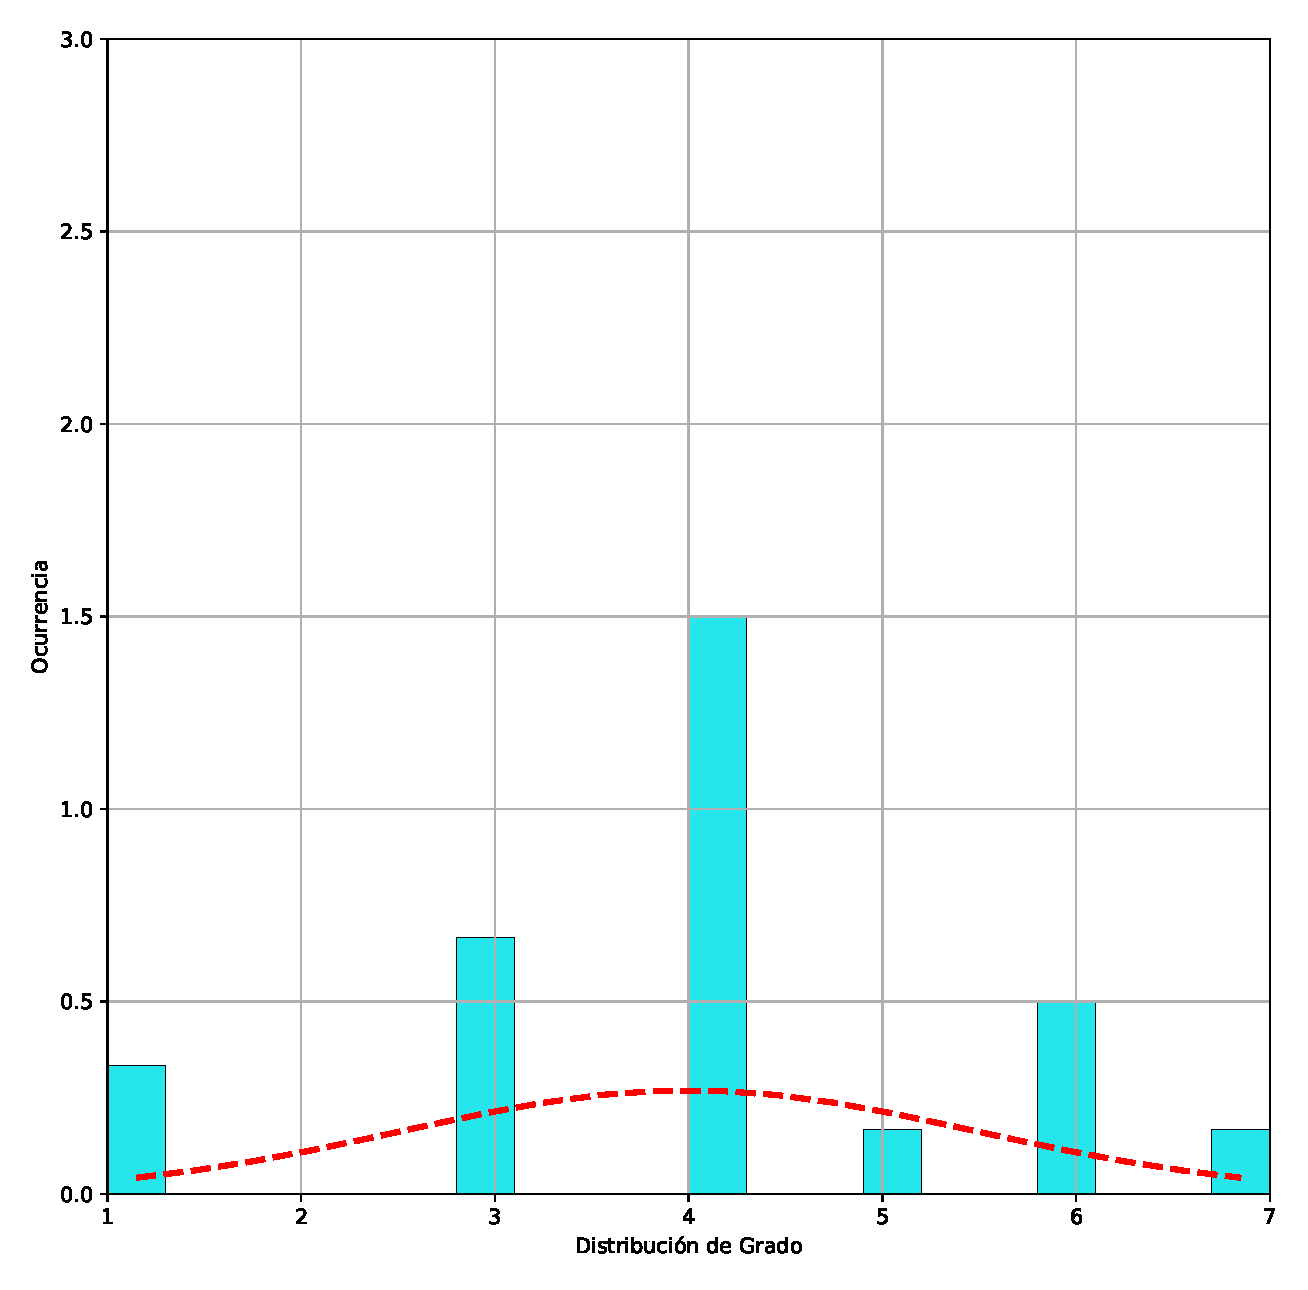
\includegraphics[scale=0.3]{GradoGrafo3D.eps}}
\subfigure[\textit{Grafo4}]{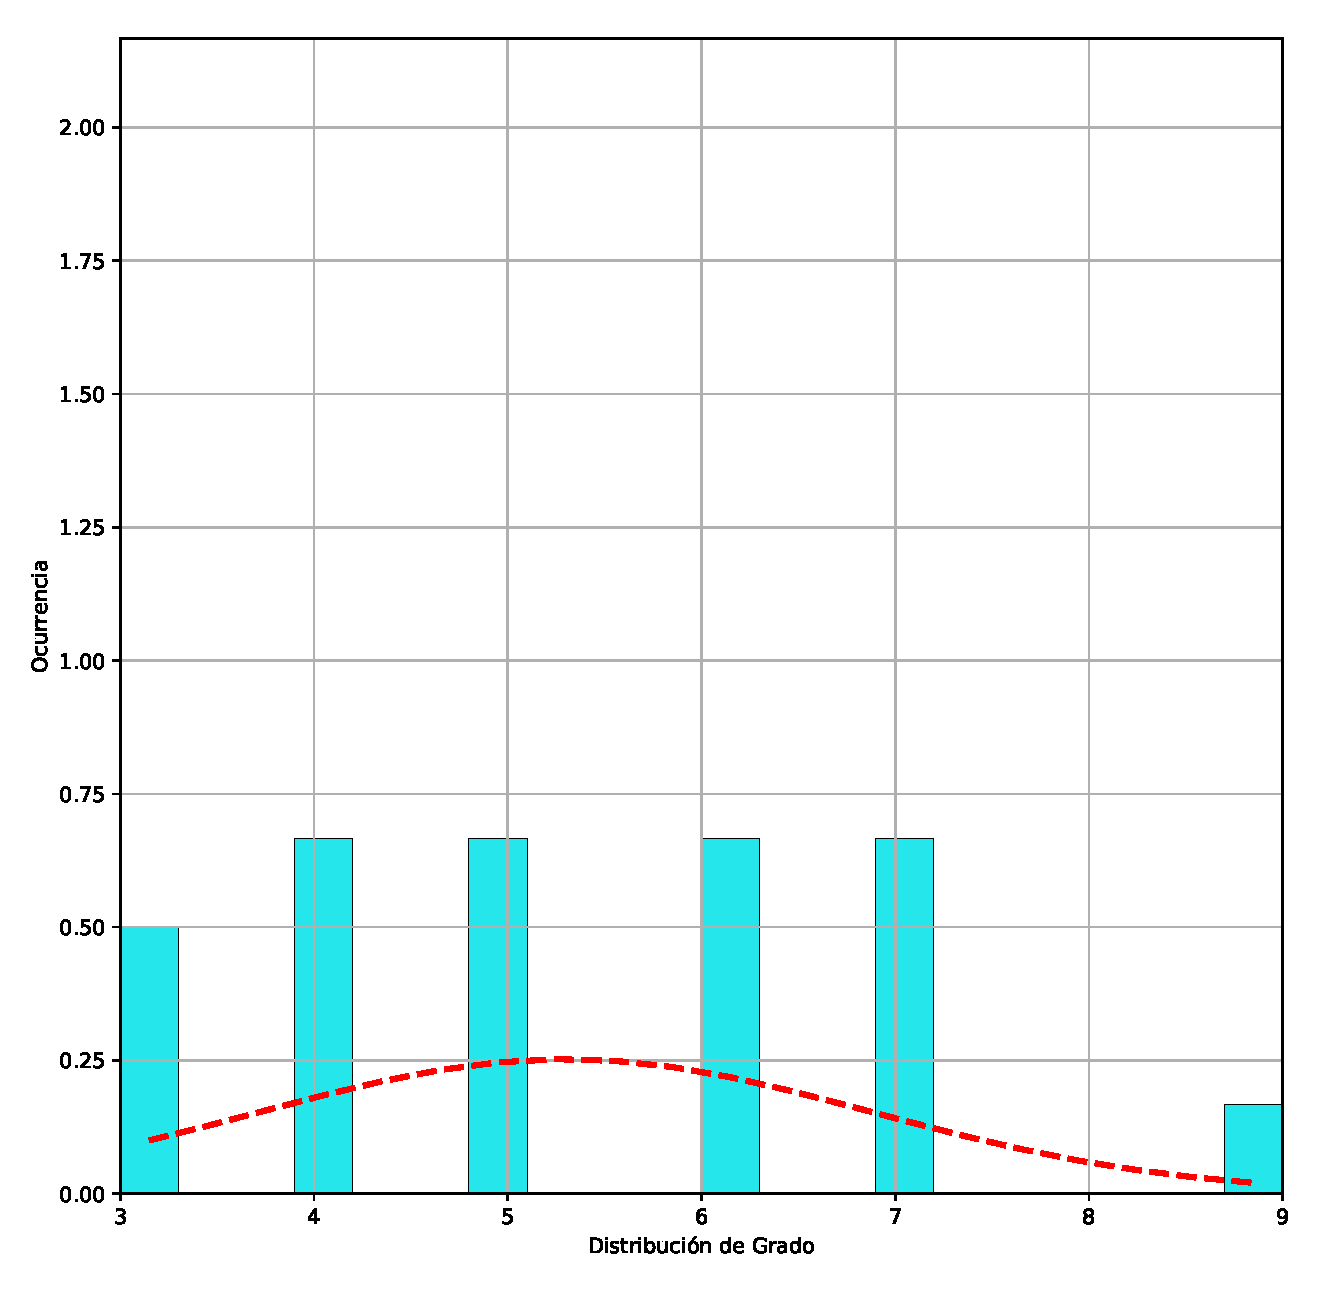
\includegraphics[scale=0.3]{GradoGrafo4D.eps}}
\subfigure[\textit{Grafo5}]{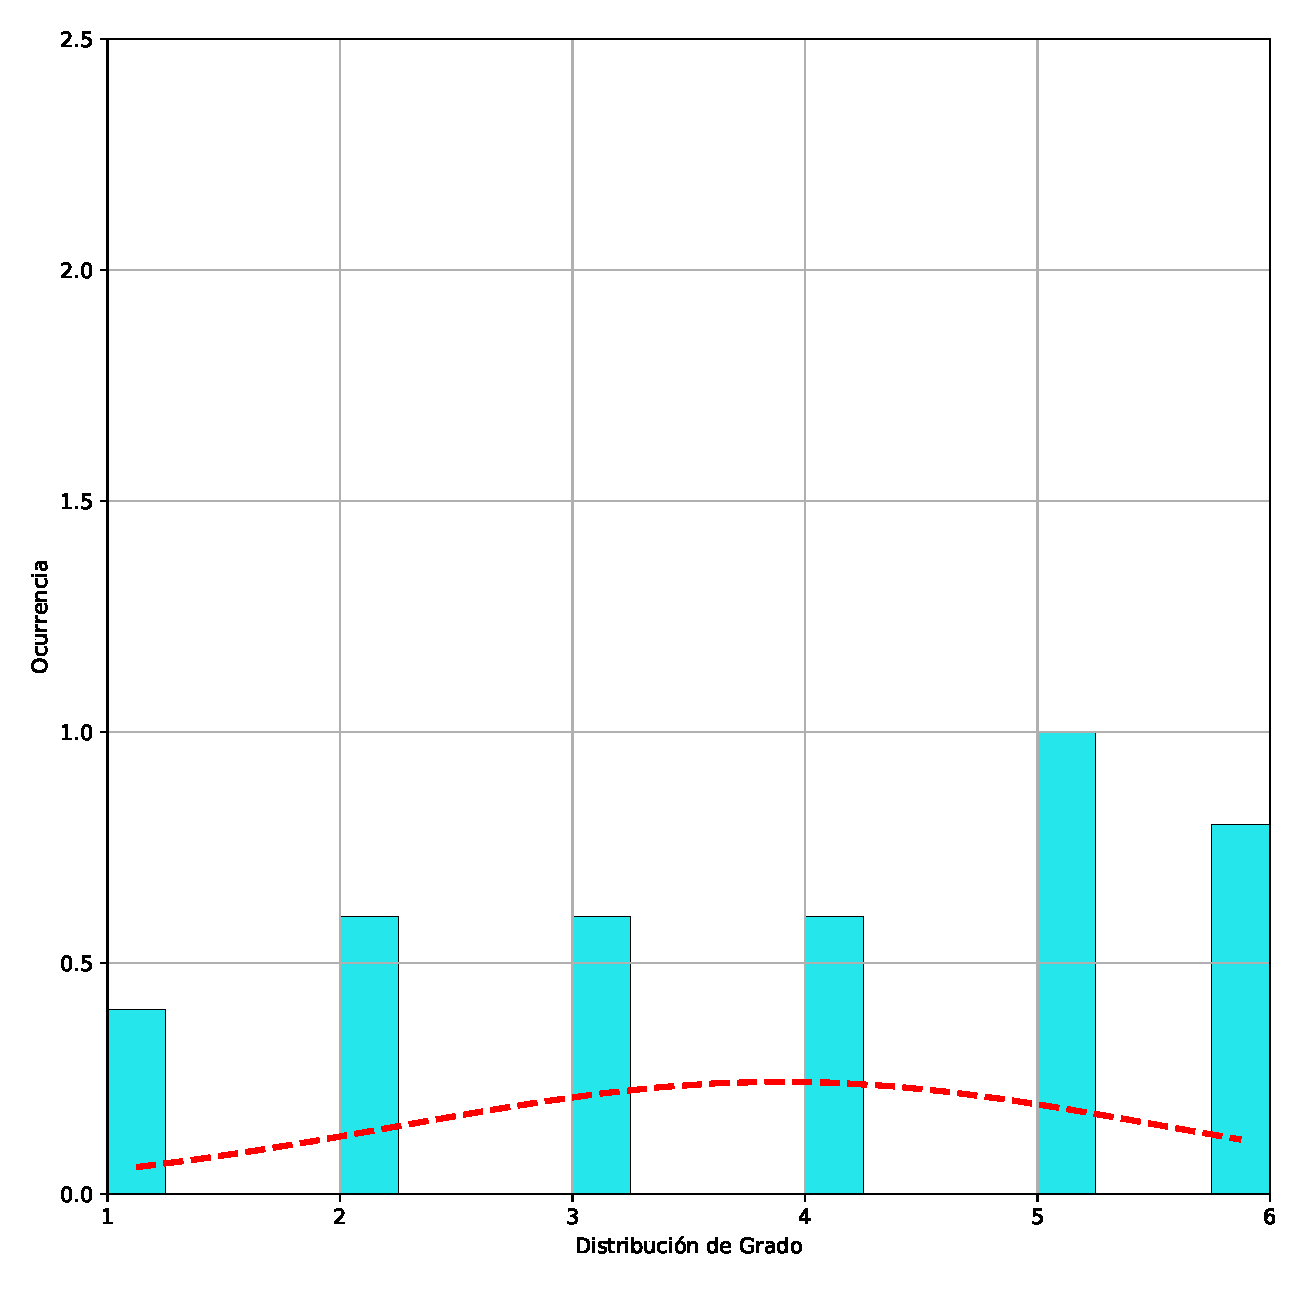
\includegraphics[scale=0.3]{GradoGrafo5D.eps}}

\caption{Histogramas que muestran la distribución de los valores de la característica distribución de grado. }
\label{fig7} 
\end{figure}

\begin{figure}[htbp]

\subfigure[\textit{Grafo1}]{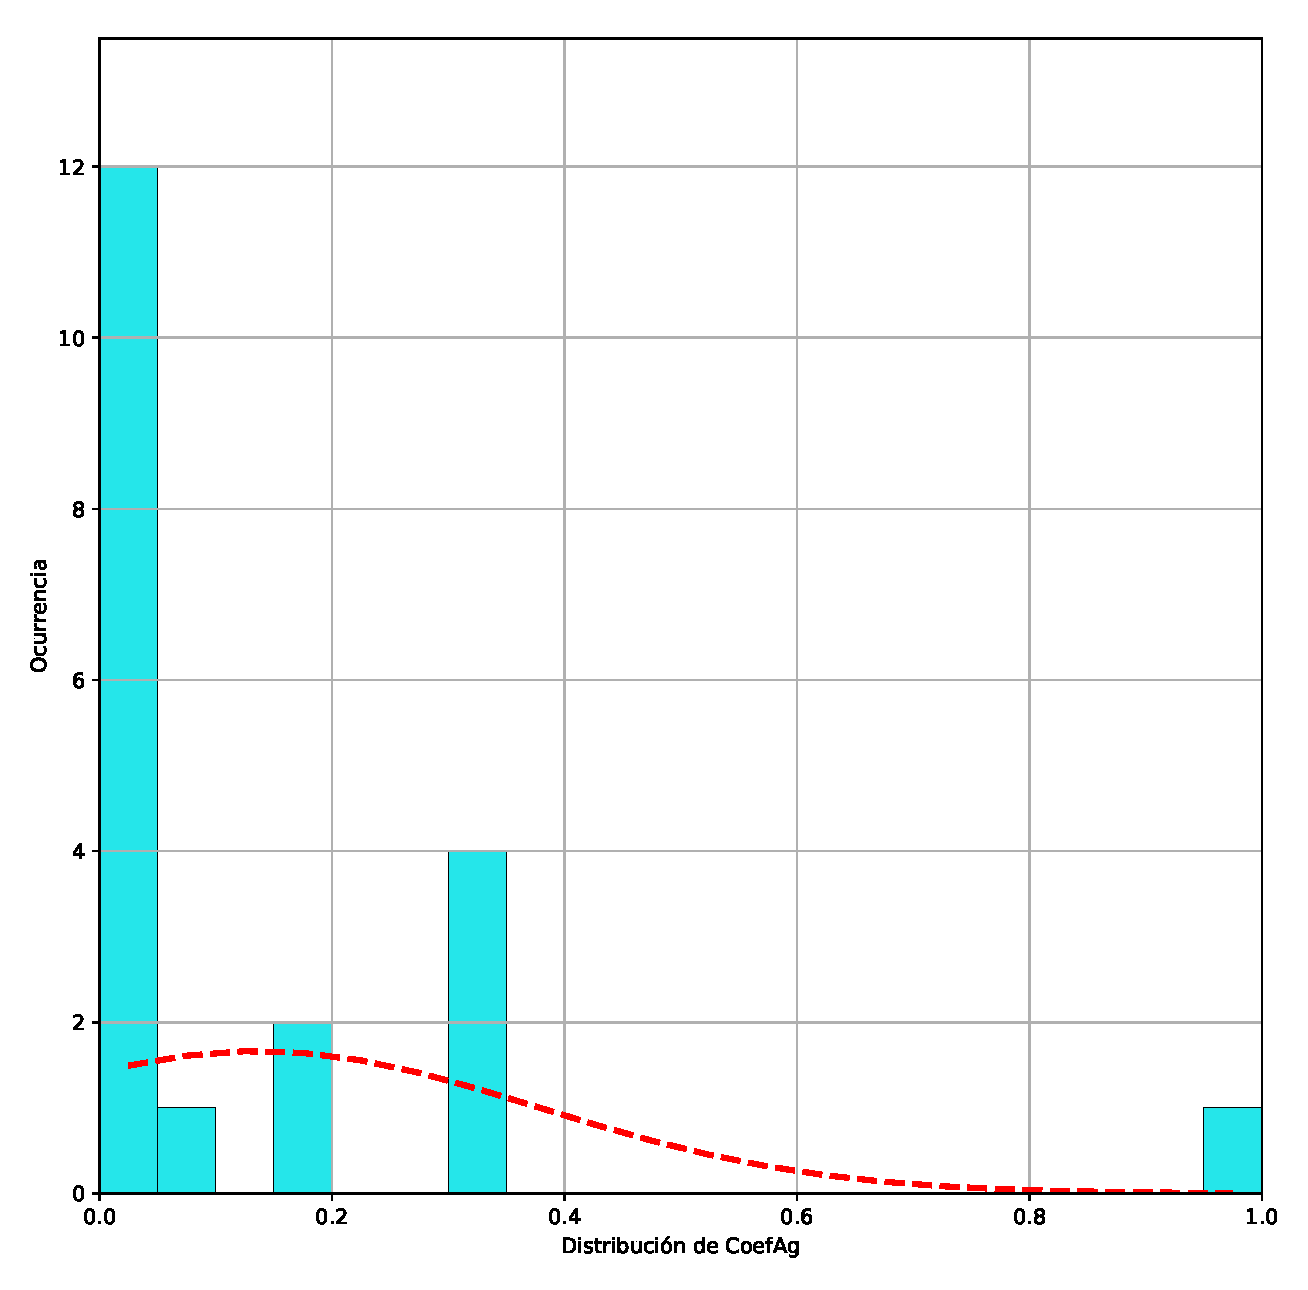
\includegraphics[scale=0.3]{CoefAgGrafo1D.eps}}
\subfigure[\textit{Grafo2}]{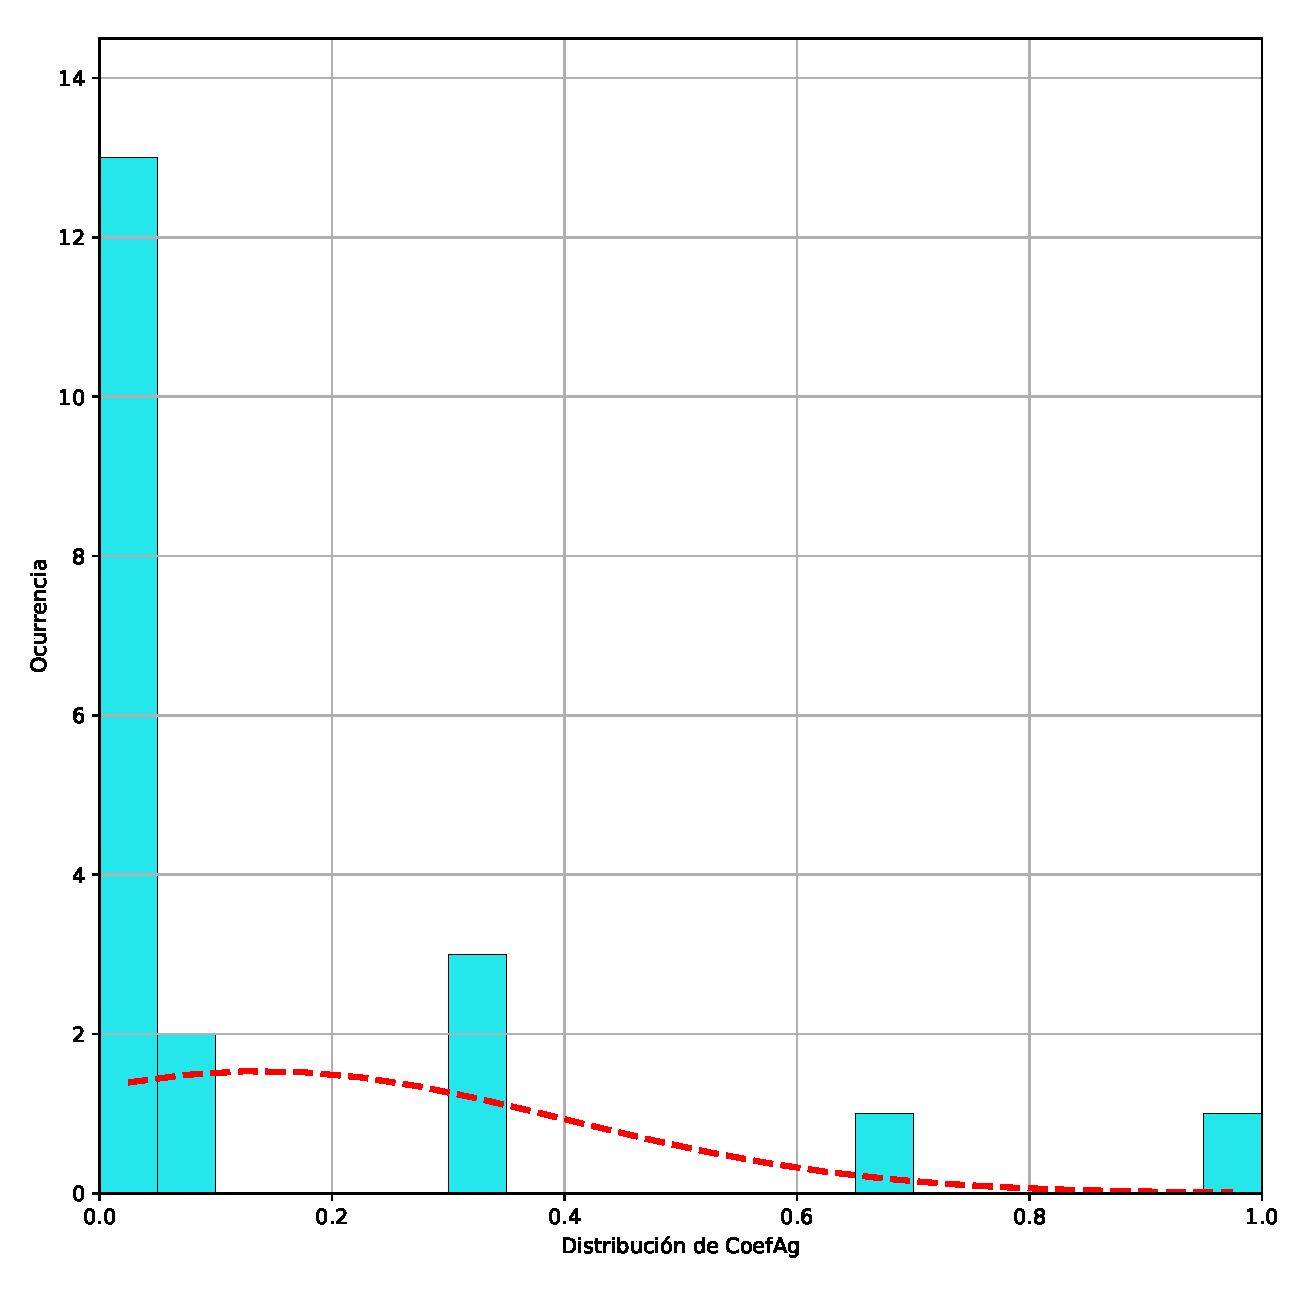
\includegraphics[scale=0.3]{CoefAgGrafo2D.eps}}
\subfigure[\textit{Grafo3}]{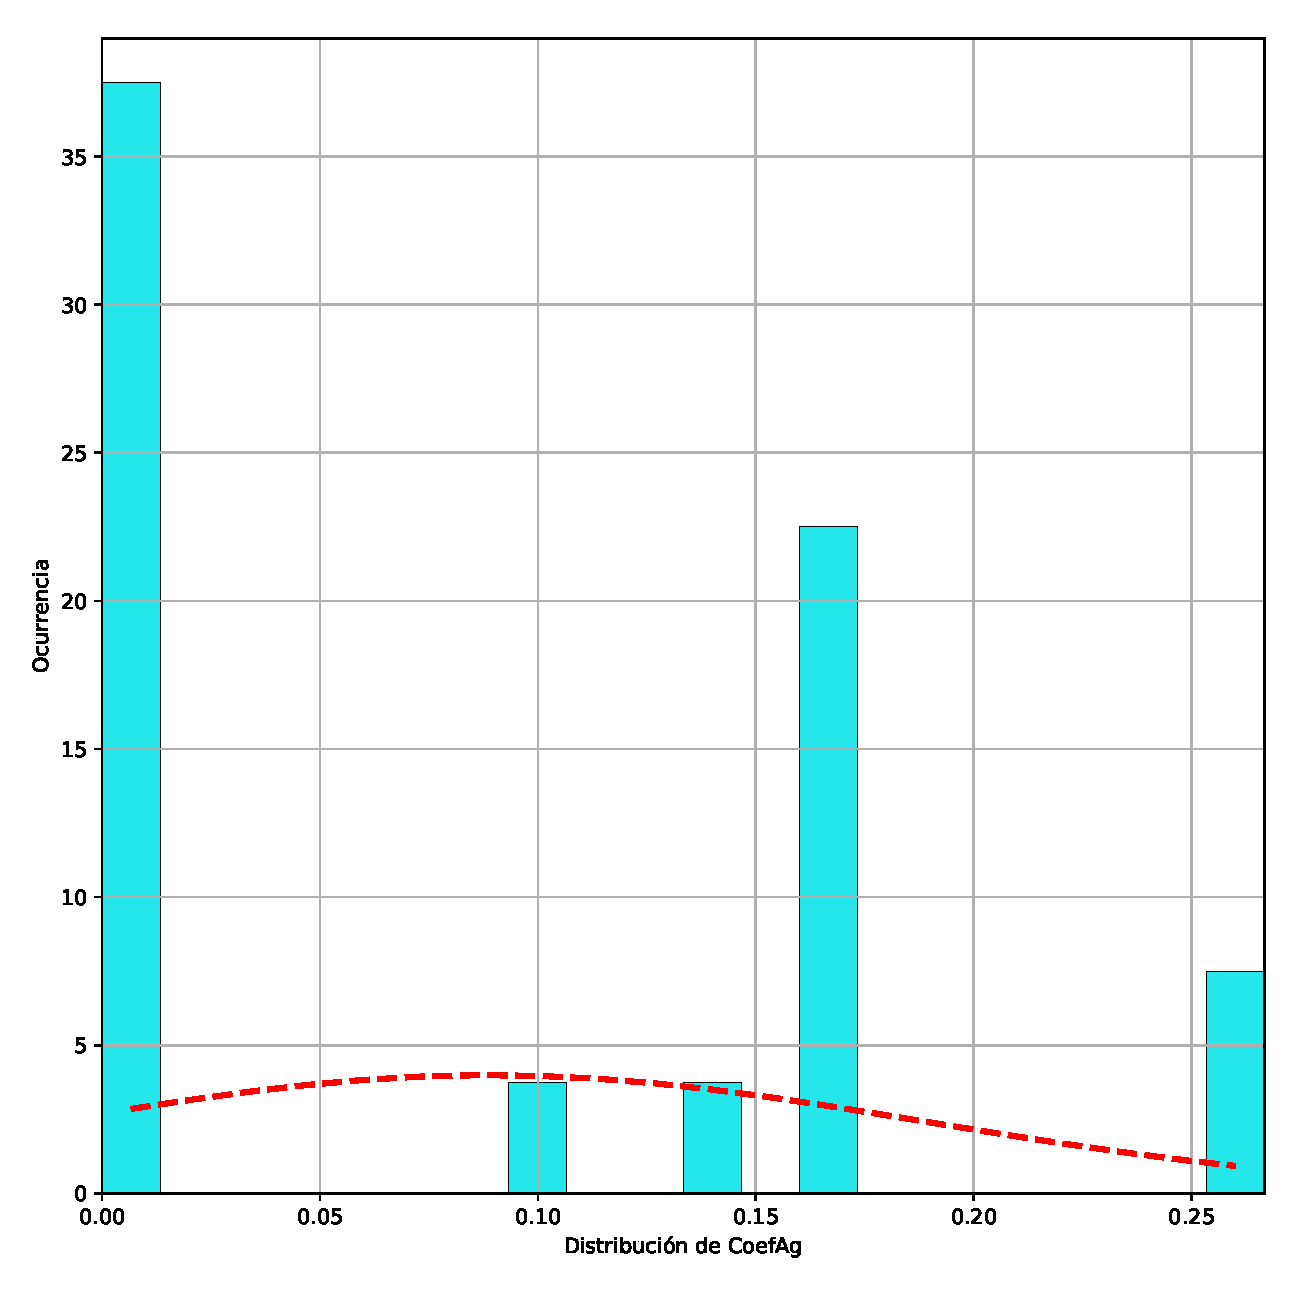
\includegraphics[scale=0.3]{CoefAgGrafo3D.eps}}
\subfigure[\textit{Grafo4}]{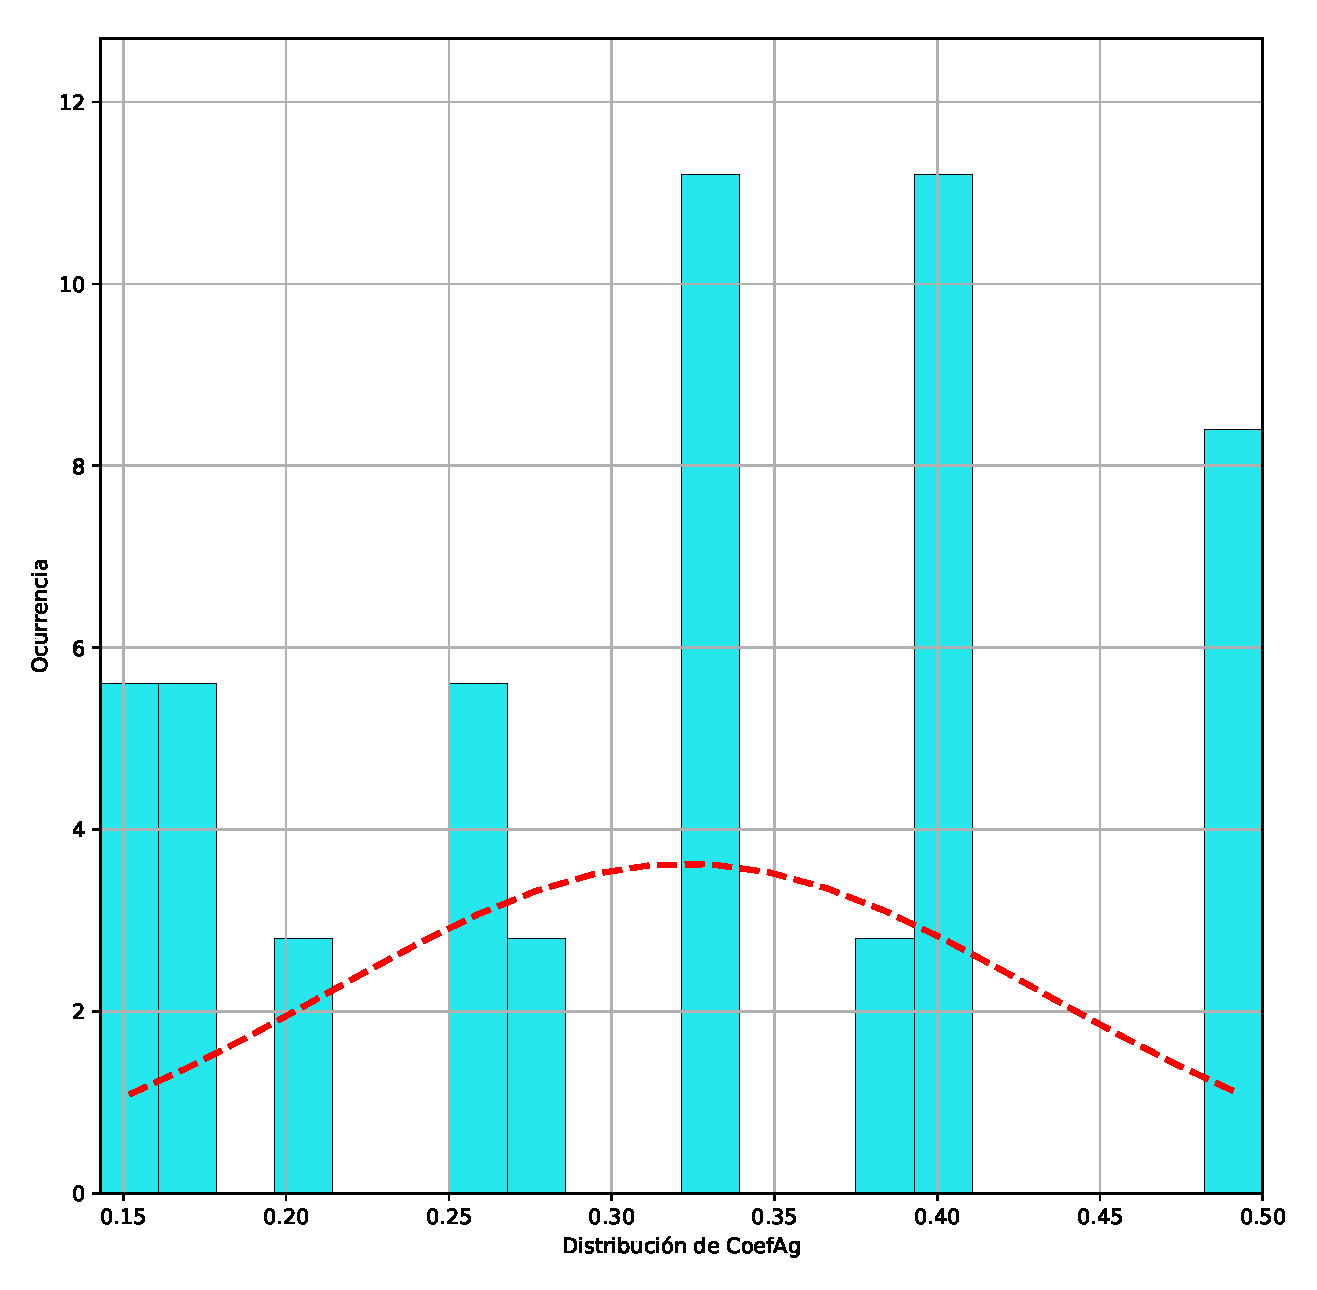
\includegraphics[scale=0.3]{CoefAgGrafo4D.eps}}
\subfigure[\textit{Grafo5}]{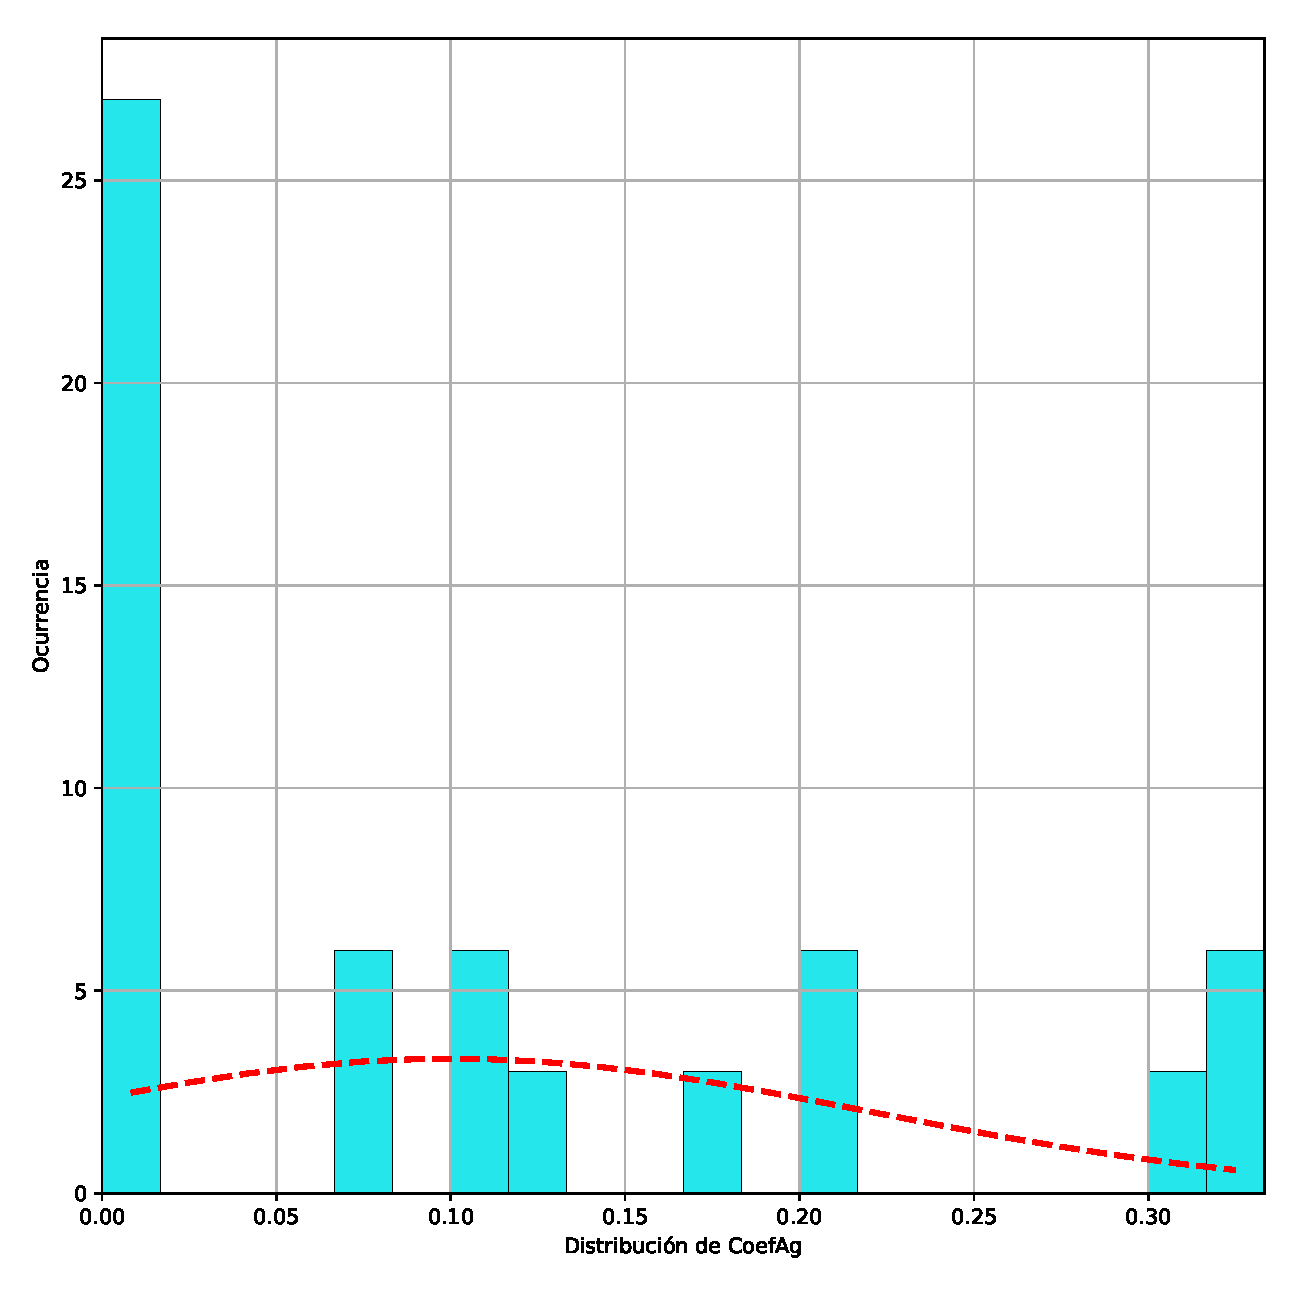
\includegraphics[scale=0.3]{CoefAgGrafo5D.eps}}

\caption{Histogramas que muestran la distribución de los valores de la característica coeficiente de agrupamiento. }
\label{fig8}
 
\end{figure}
\begin{figure}[htbp]

\subfigure[\textit{Grafo1}]{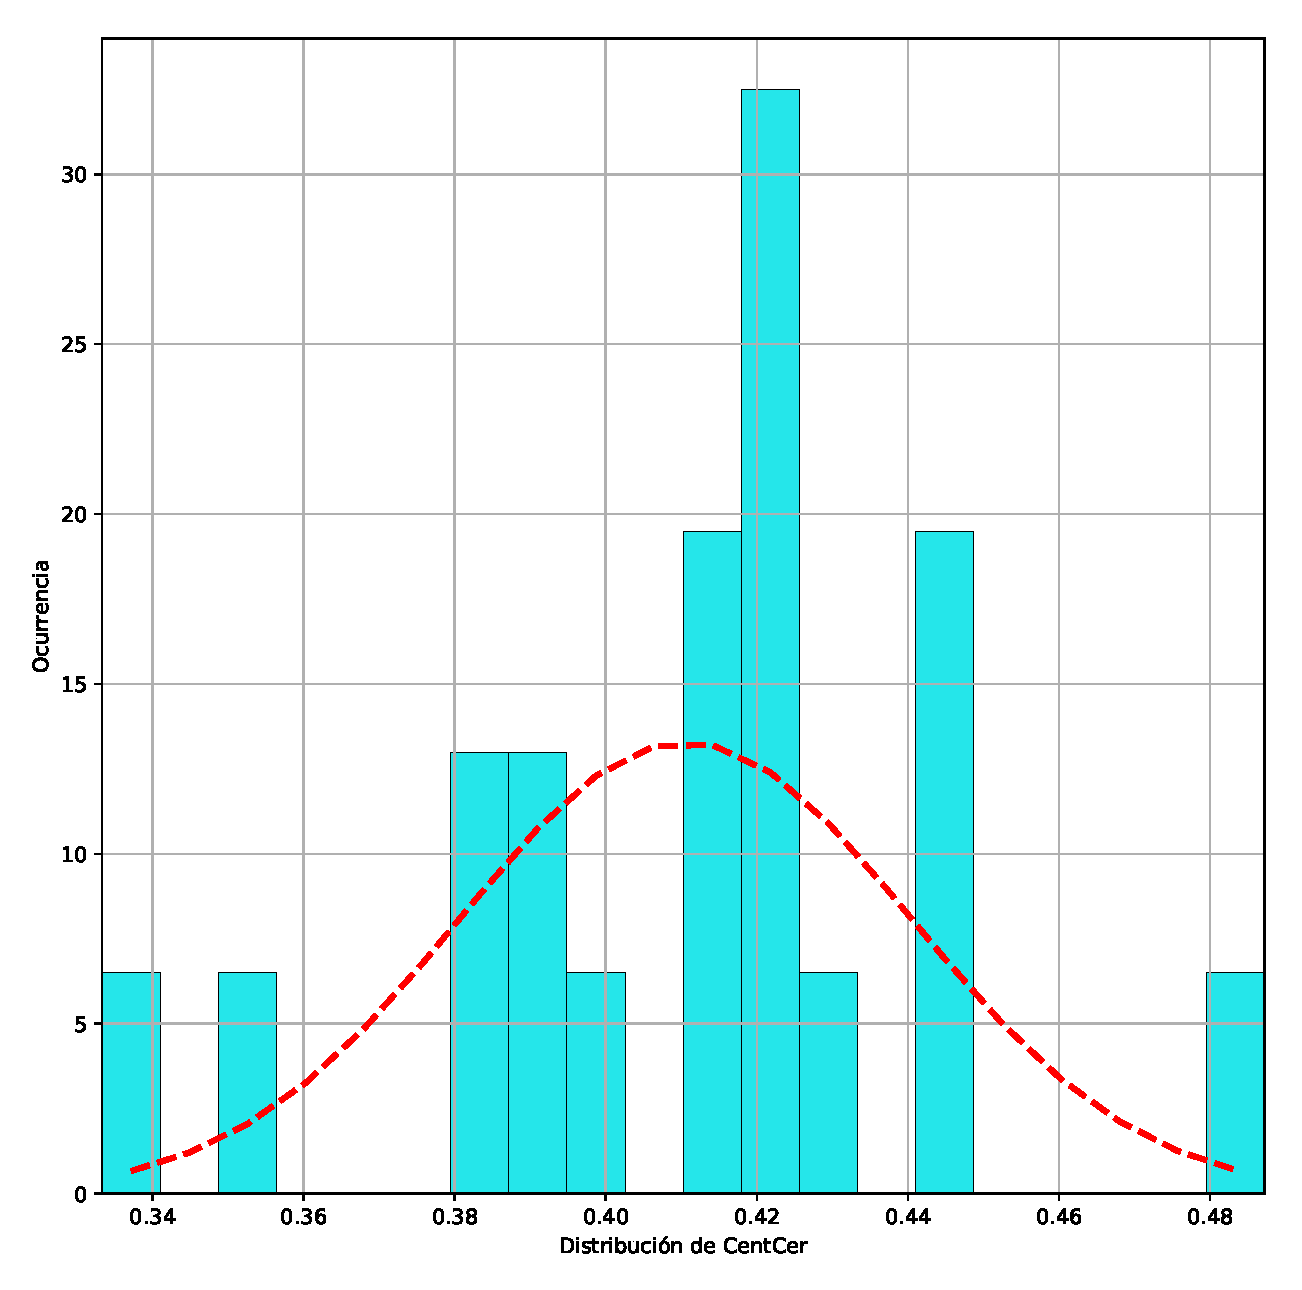
\includegraphics[scale=0.3]{CentCerGrafo1D.eps}}
\subfigure[\textit{Grafo2}]{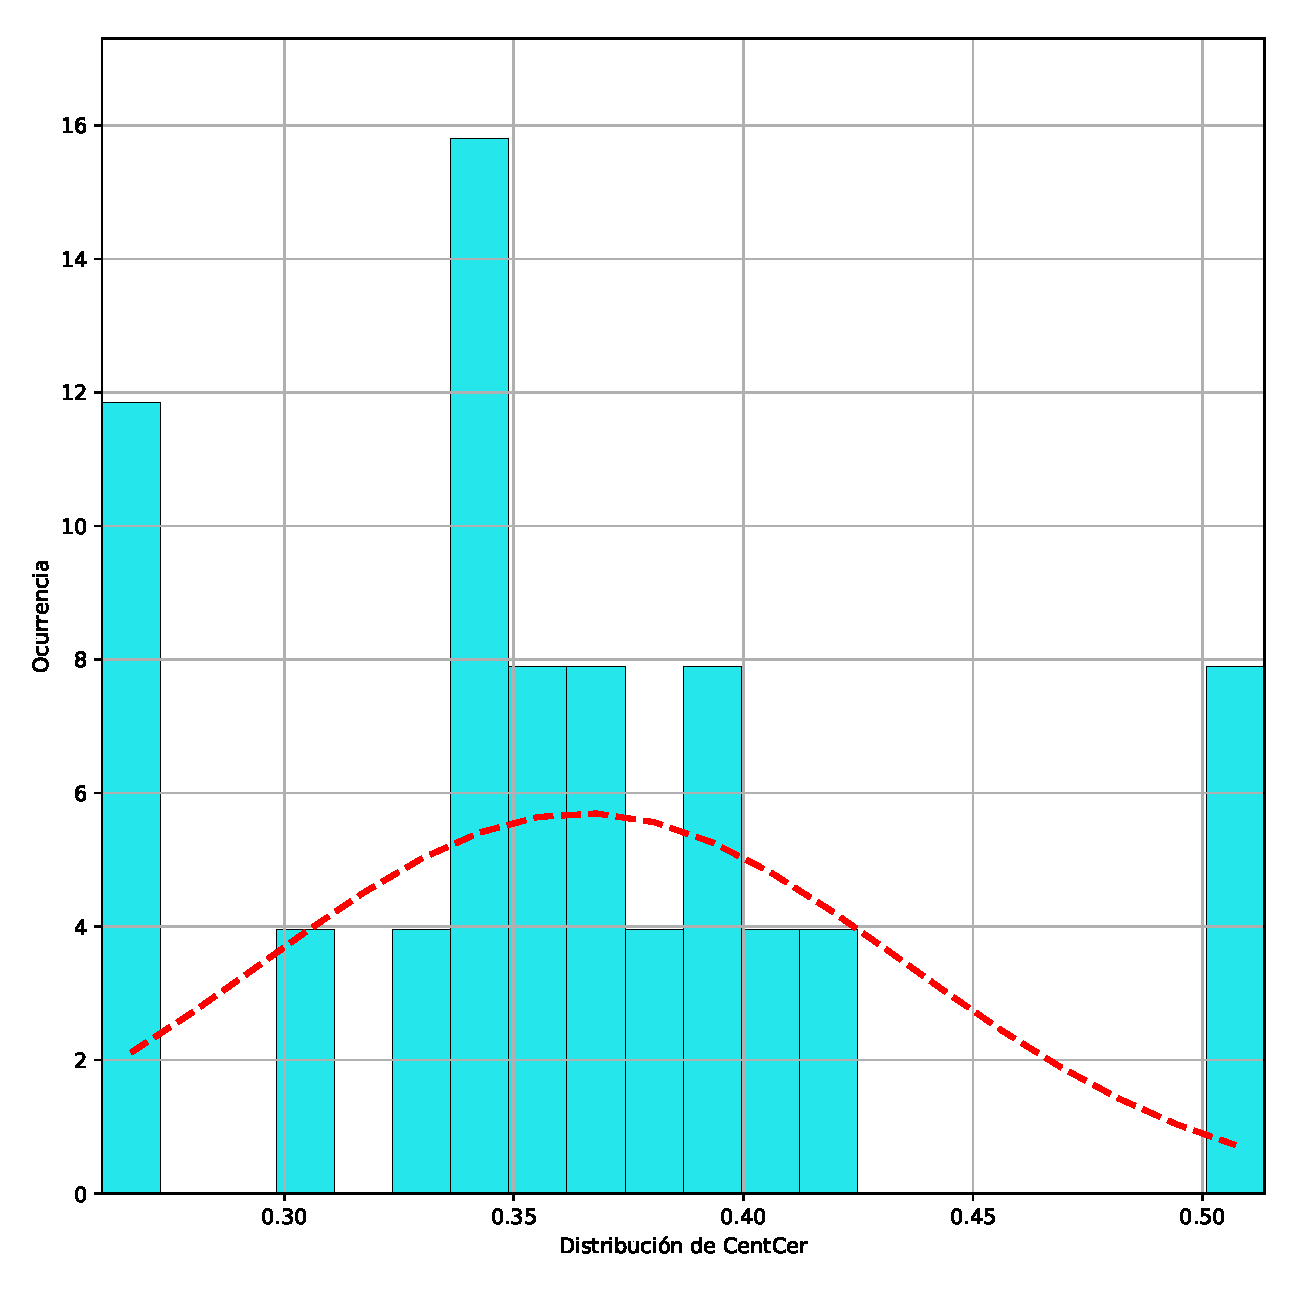
\includegraphics[scale=0.3]{CentCerGrafo2D.eps}}
\subfigure[\textit{Grafo3}]{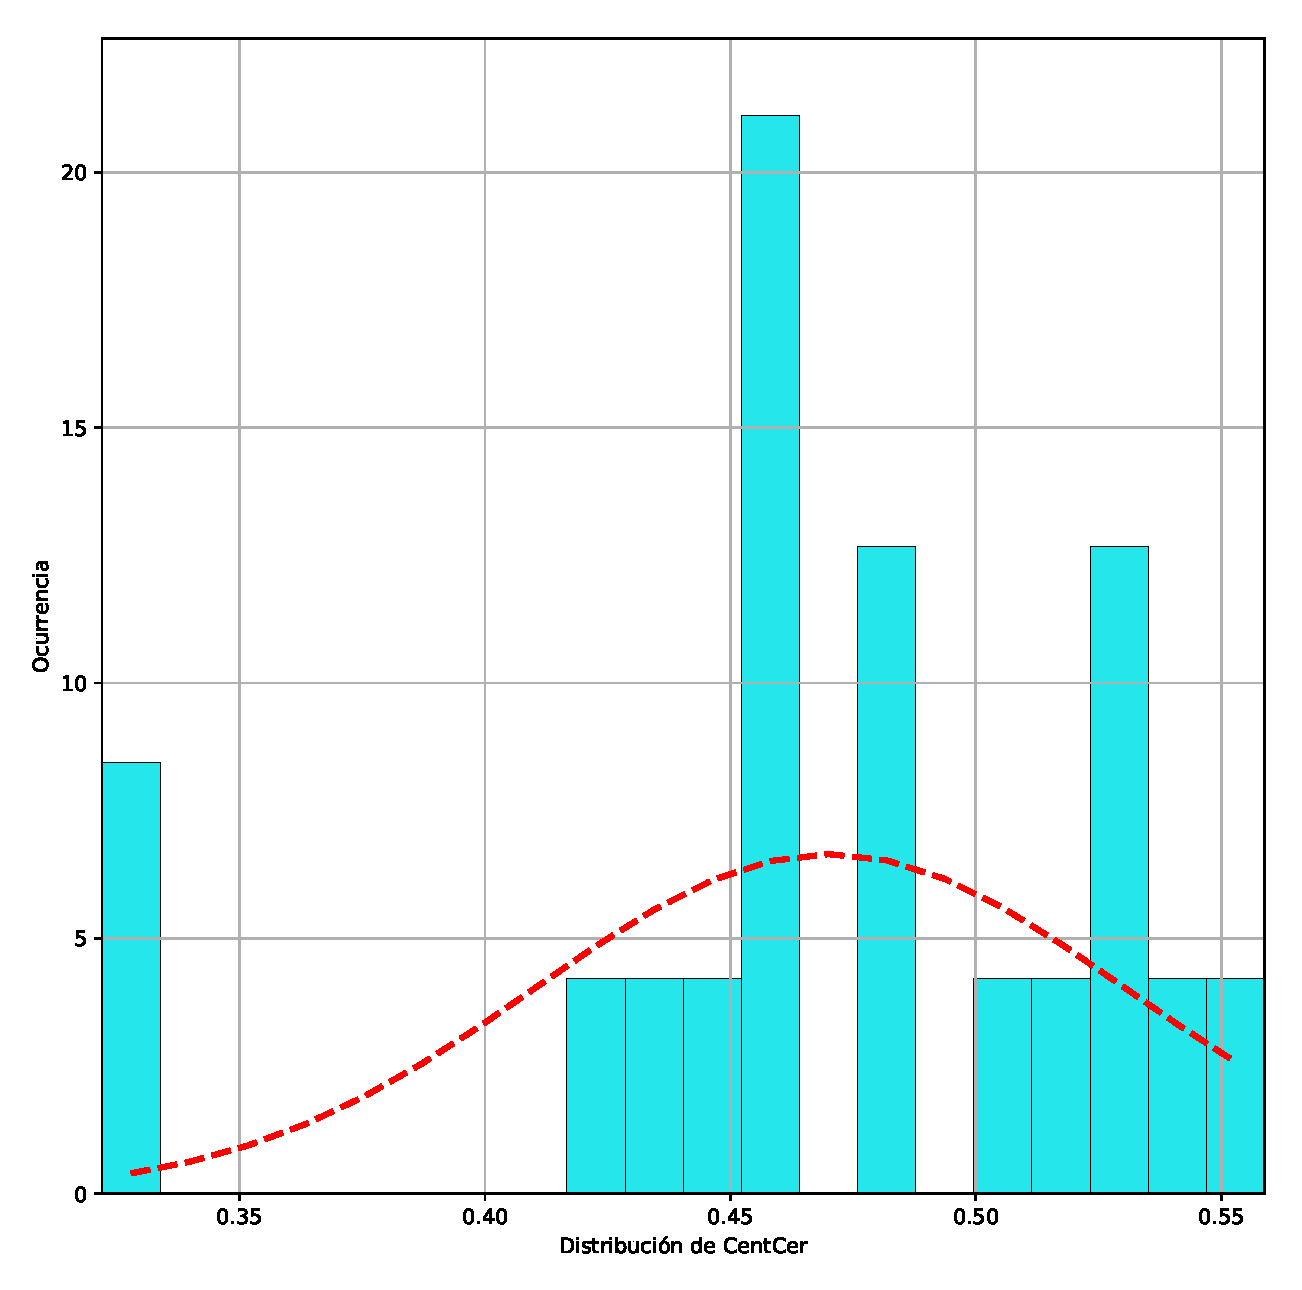
\includegraphics[scale=0.3]{CentCerGrafo3D.eps}}
\subfigure[\textit{Grafo4}]{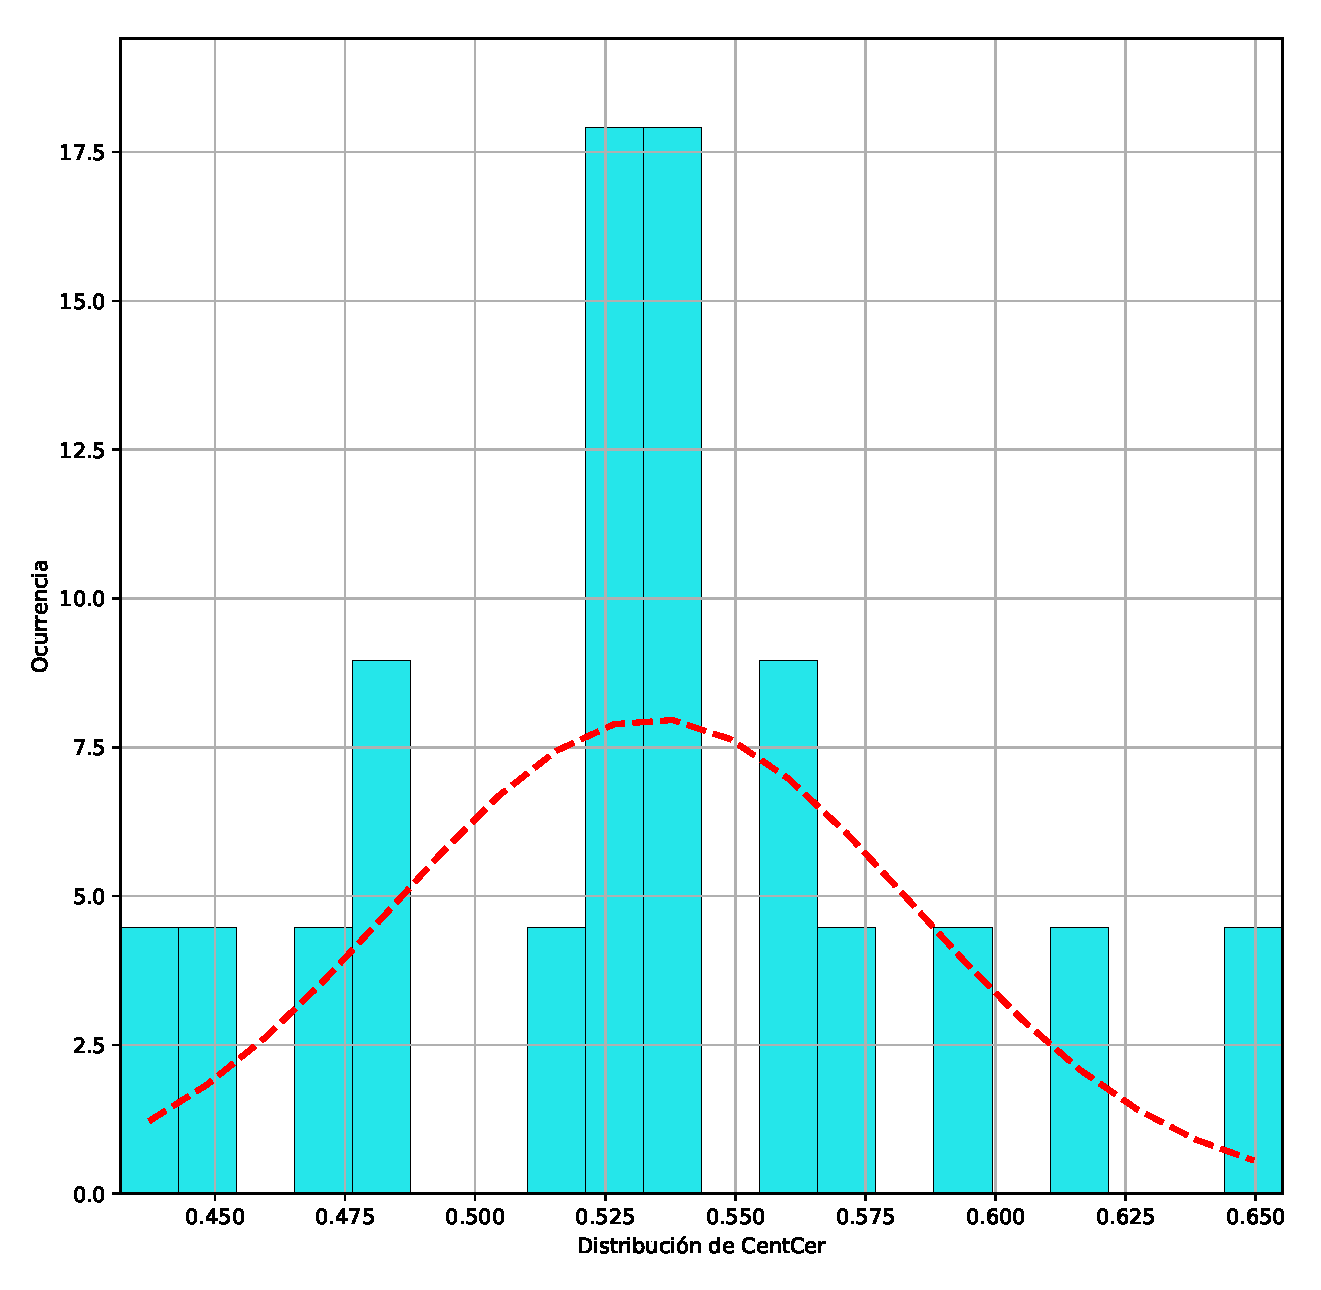
\includegraphics[scale=0.3]{CentCerGrafo4D.eps}}
\subfigure[\textit{Grafo5}]{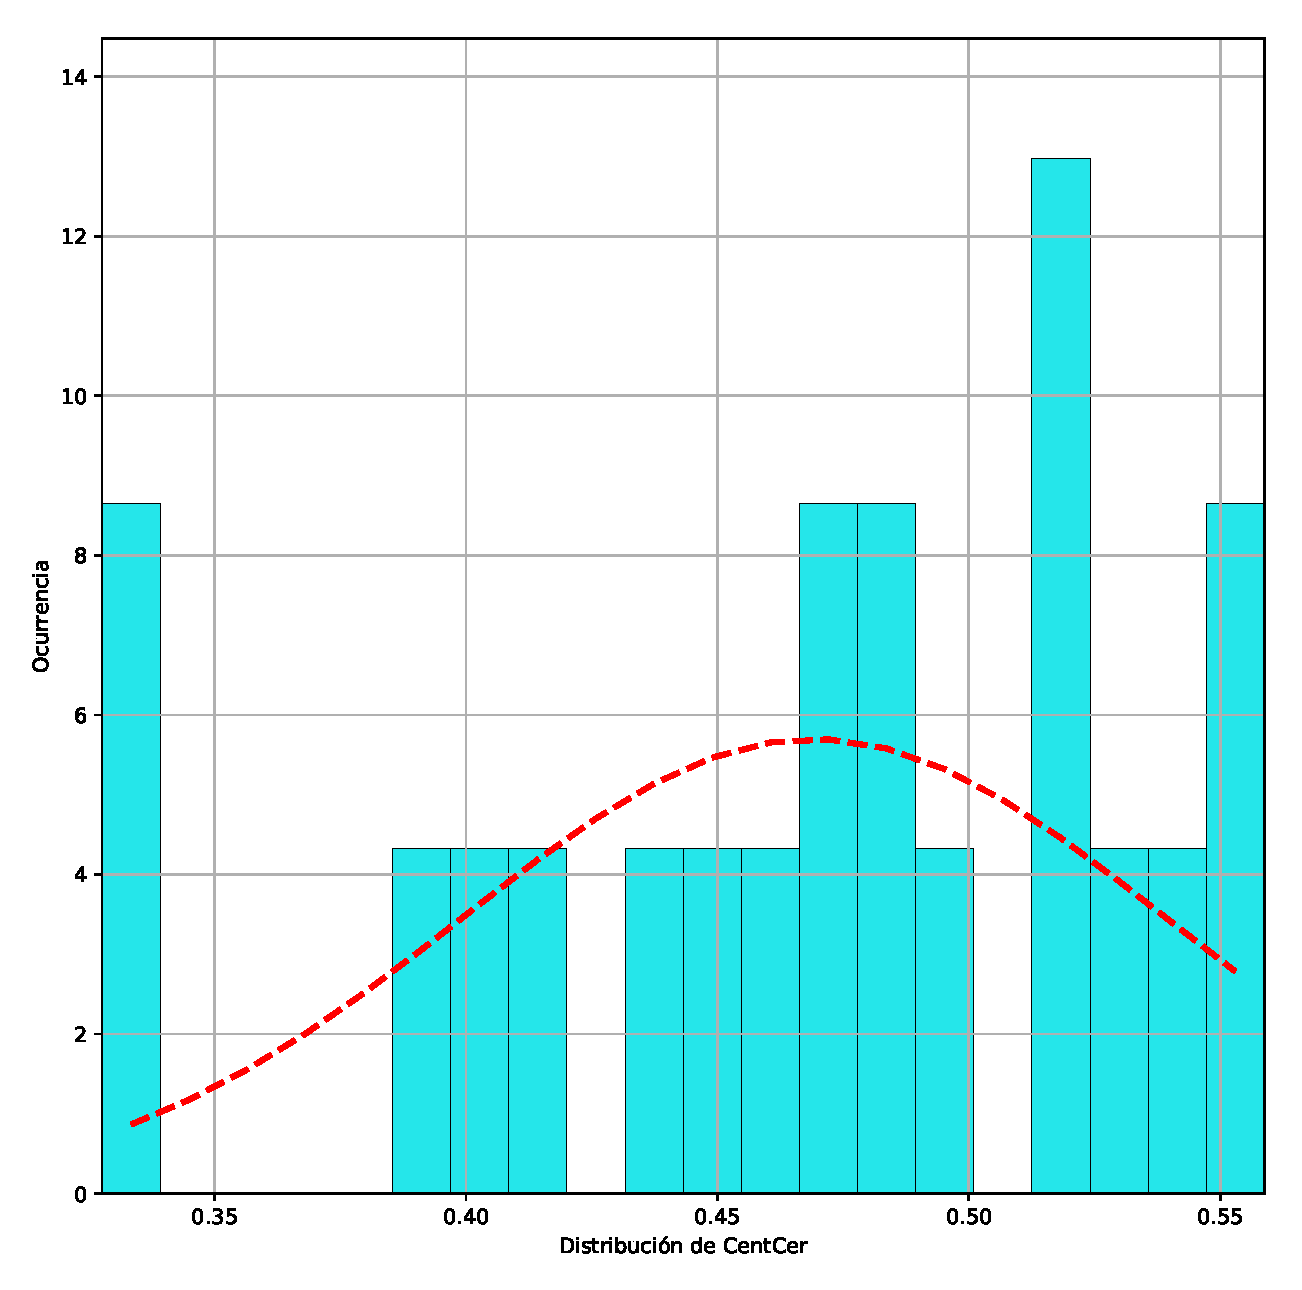
\includegraphics[scale=0.3]{CentCerGrafo5D.eps}}

\caption{Histogramas que muestran la distribución de los valores de la característica centralidad de cercanía. }
\label{fig9} 
\end{figure}

\begin{figure}[htbp]

\subfigure[\textit{Grafo1}]{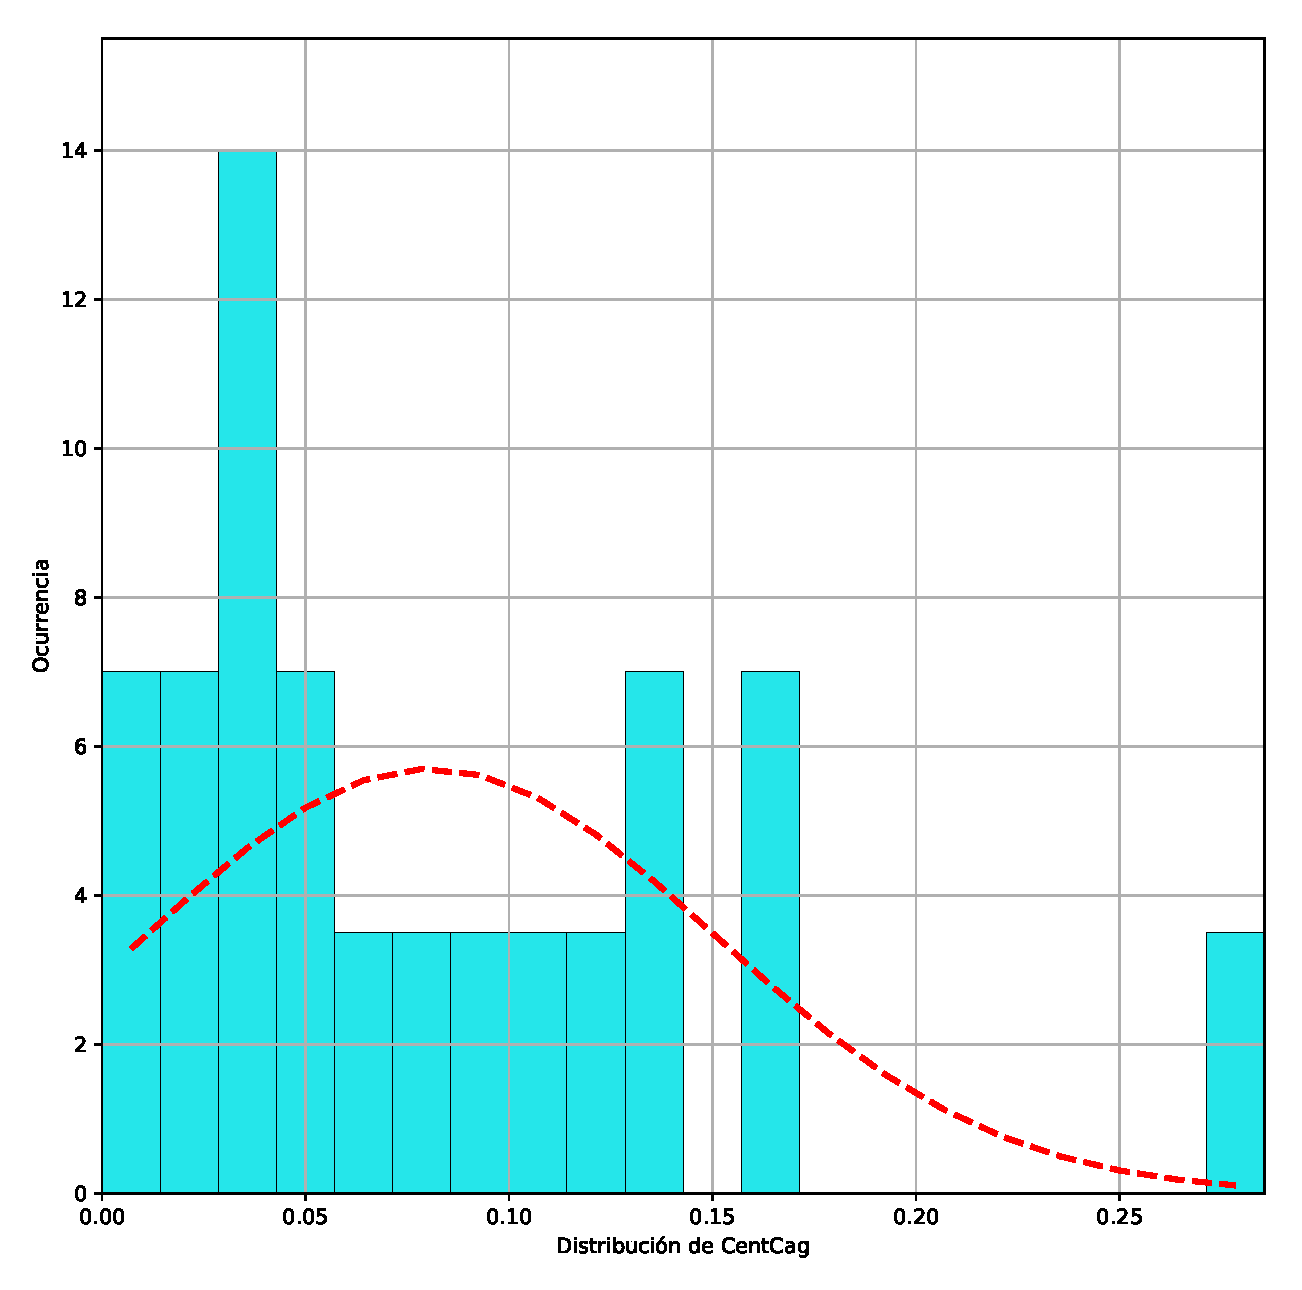
\includegraphics[scale=0.3]{CentCagGrafo1D.eps}}
\subfigure[\textit{Grafo2}]{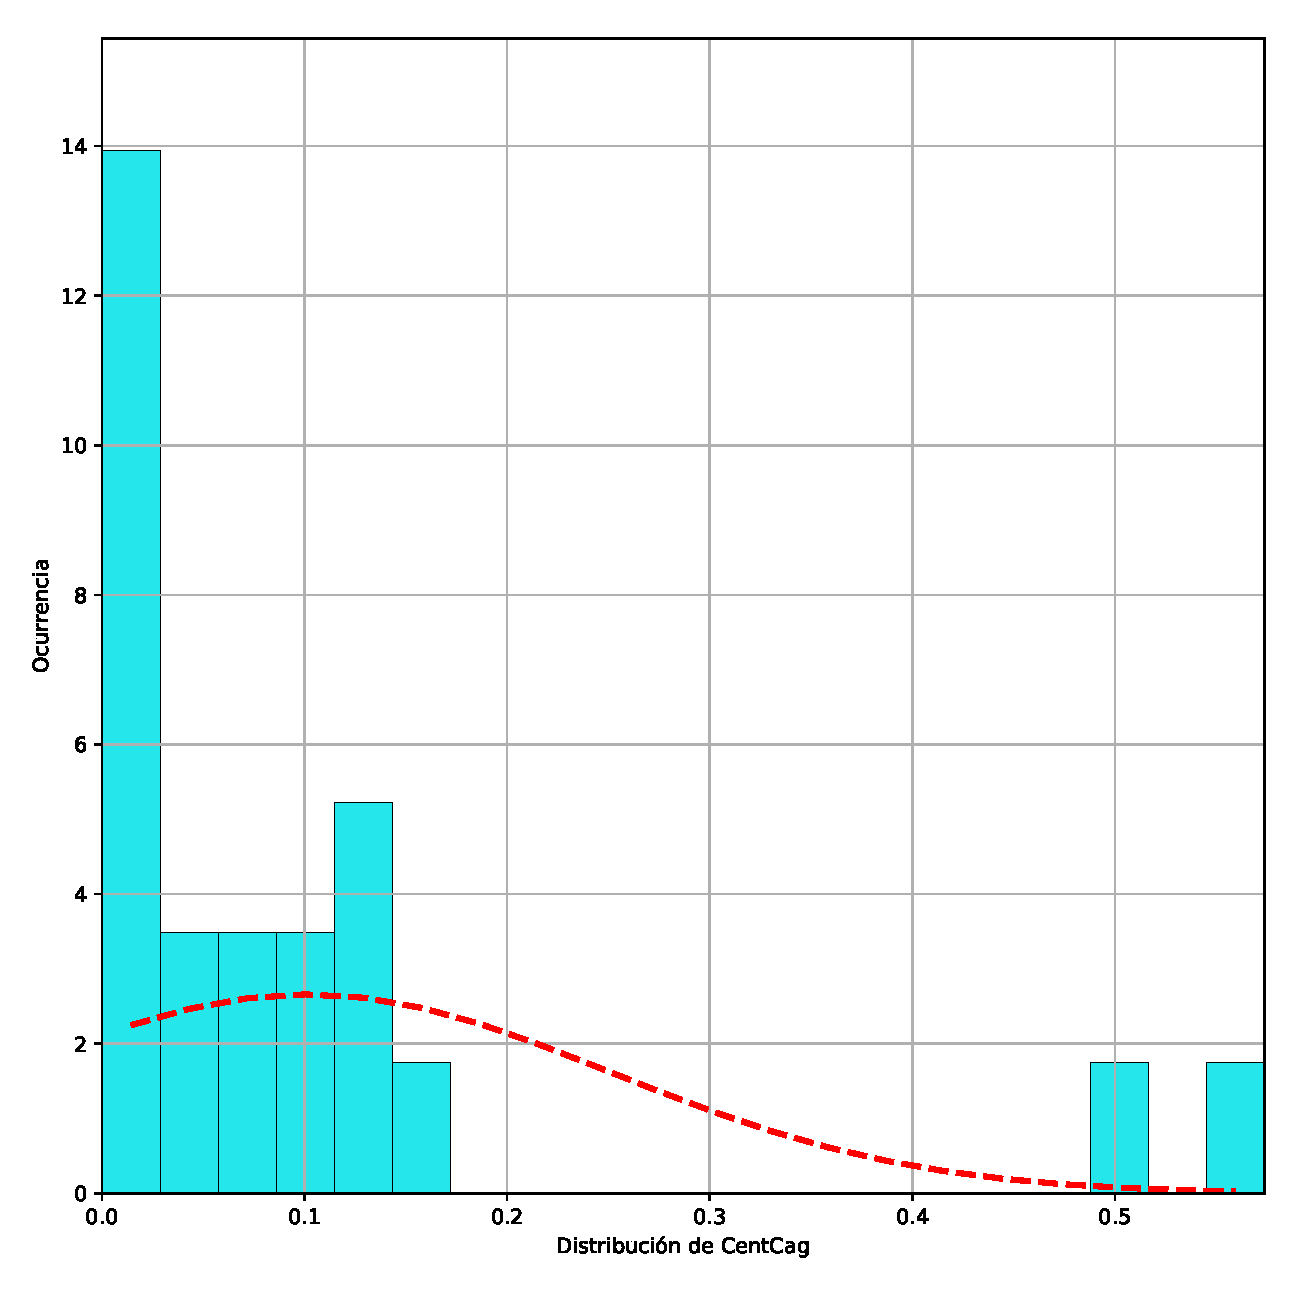
\includegraphics[scale=0.3]{CentCagGrafo2D.eps}}
\subfigure[\textit{Grafo3}]{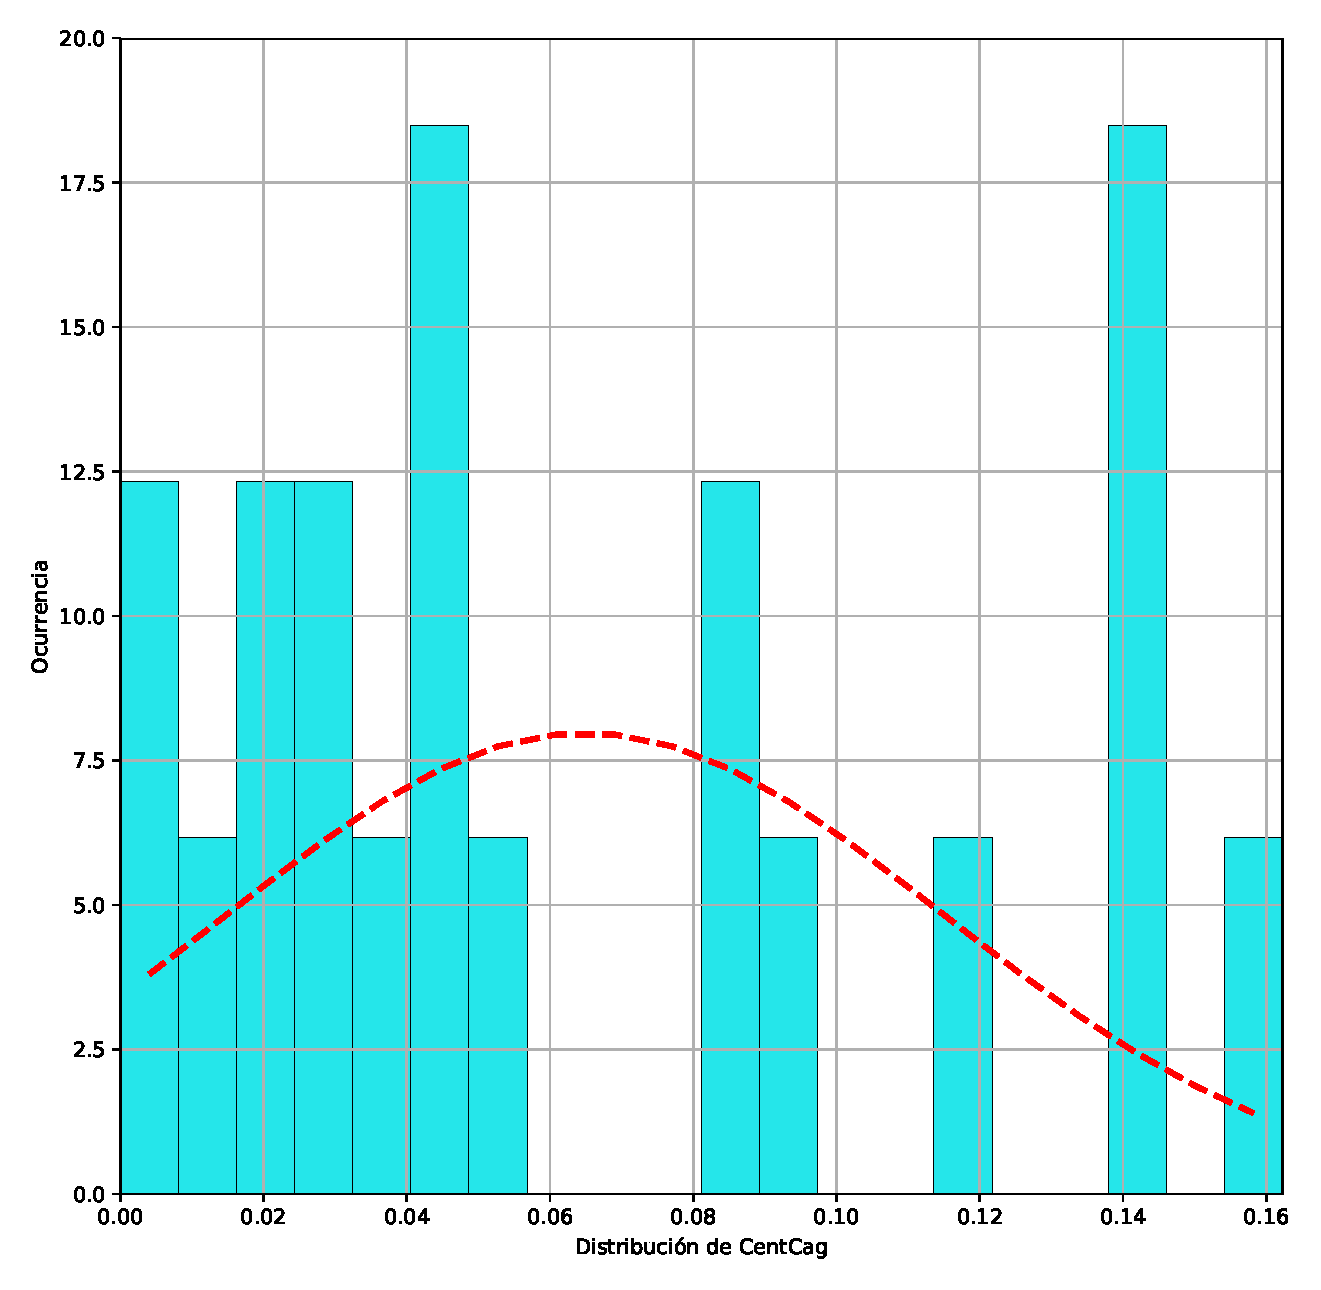
\includegraphics[scale=0.3]{CentCagGrafo3D.eps}}
\subfigure[\textit{Grafo4}]{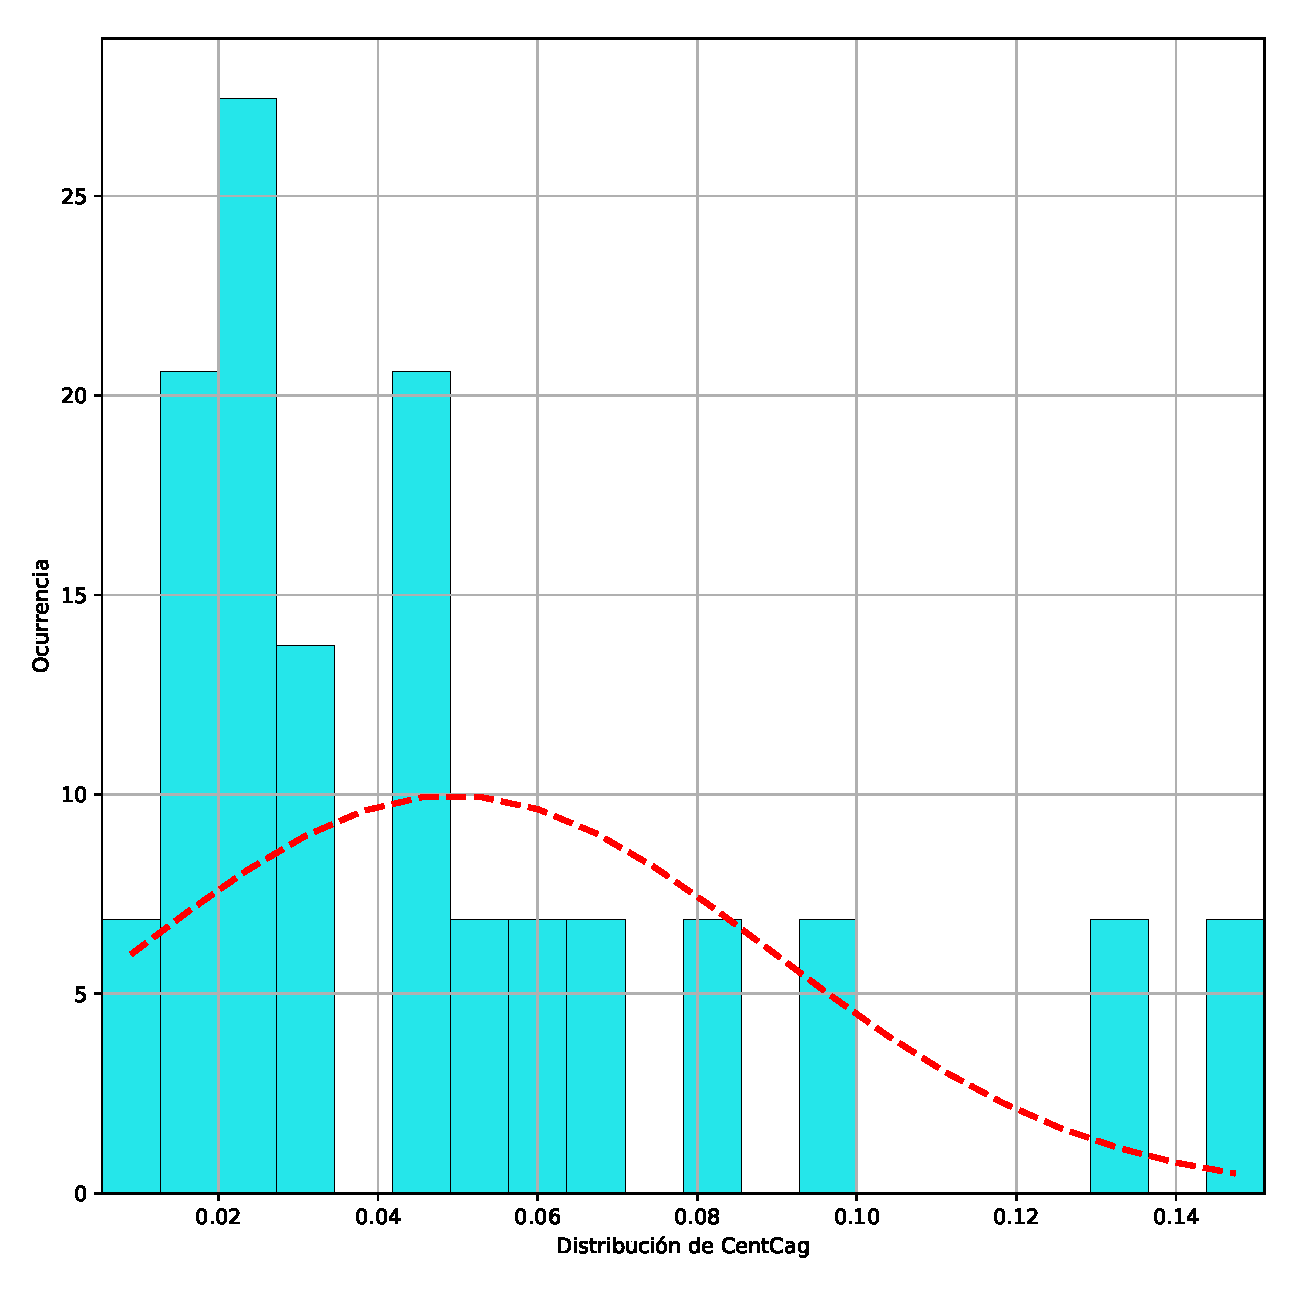
\includegraphics[scale=0.3]{CentCagGrafo4D.eps}}
\subfigure[\textit{Grafo5}]{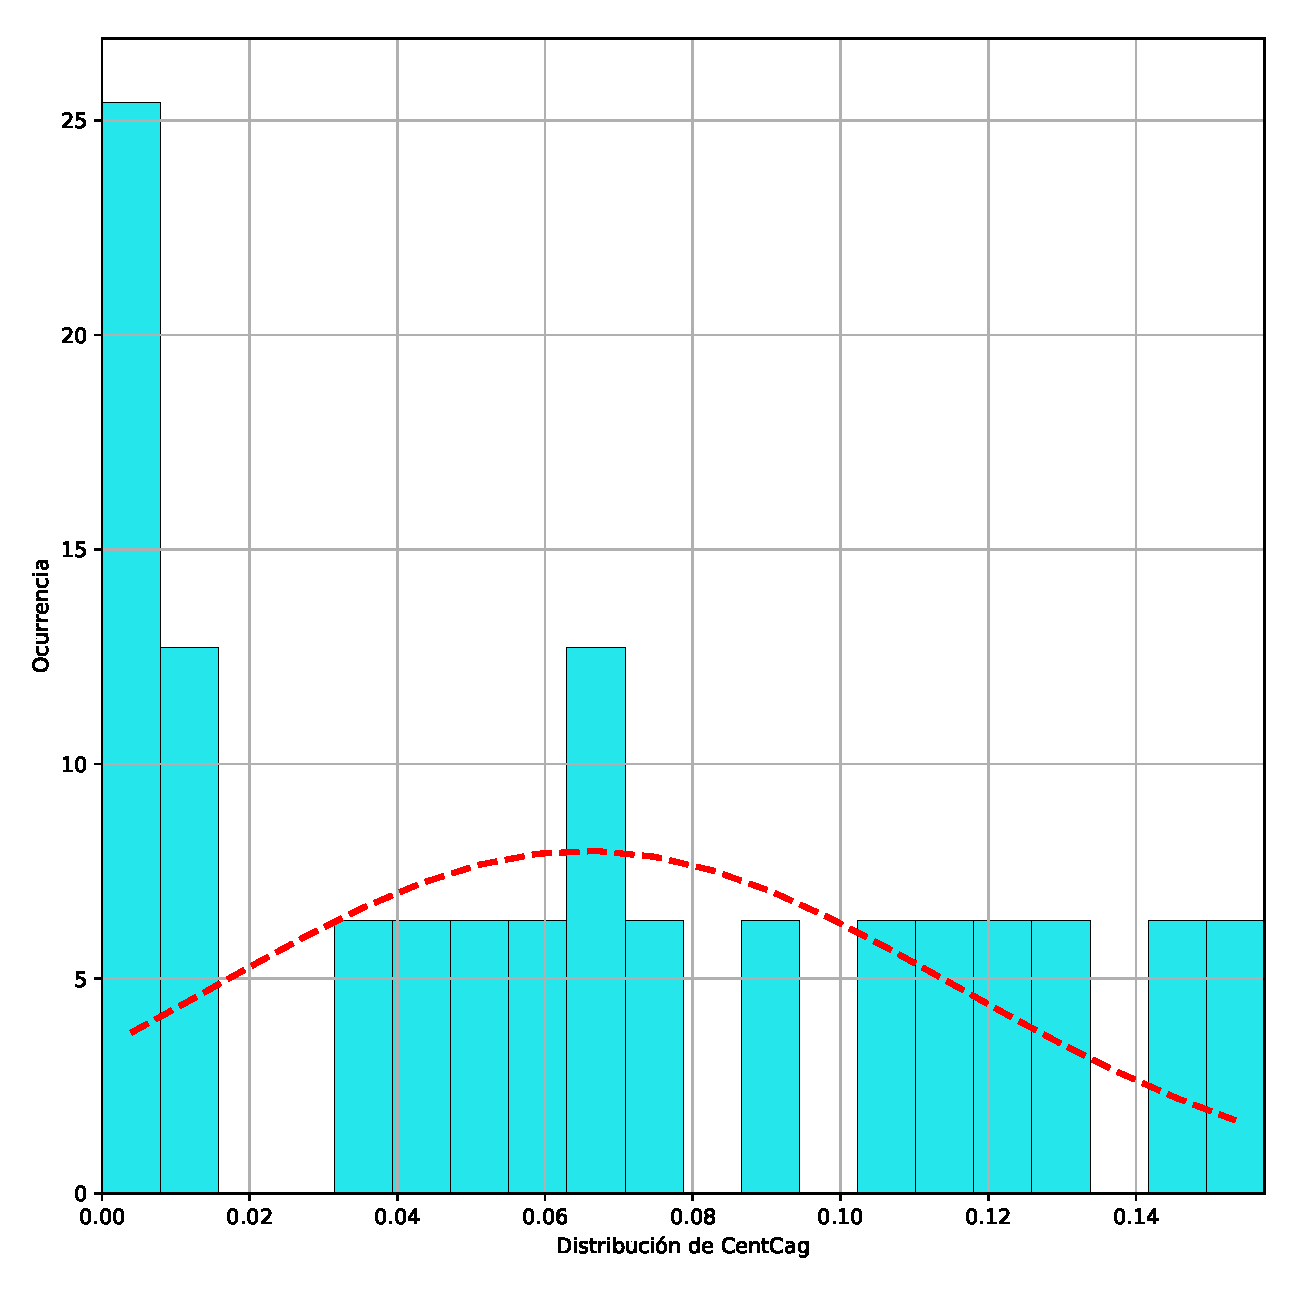
\includegraphics[scale=0.3]{CentCagGrafo5D.eps}}

\caption{Histogramas que muestran la distribución de los valores de la característica centralidad de carga. }
\label{fig10} 
\end{figure}

\begin{figure}[htbp]

\subfigure[\textit{Grafo1}]{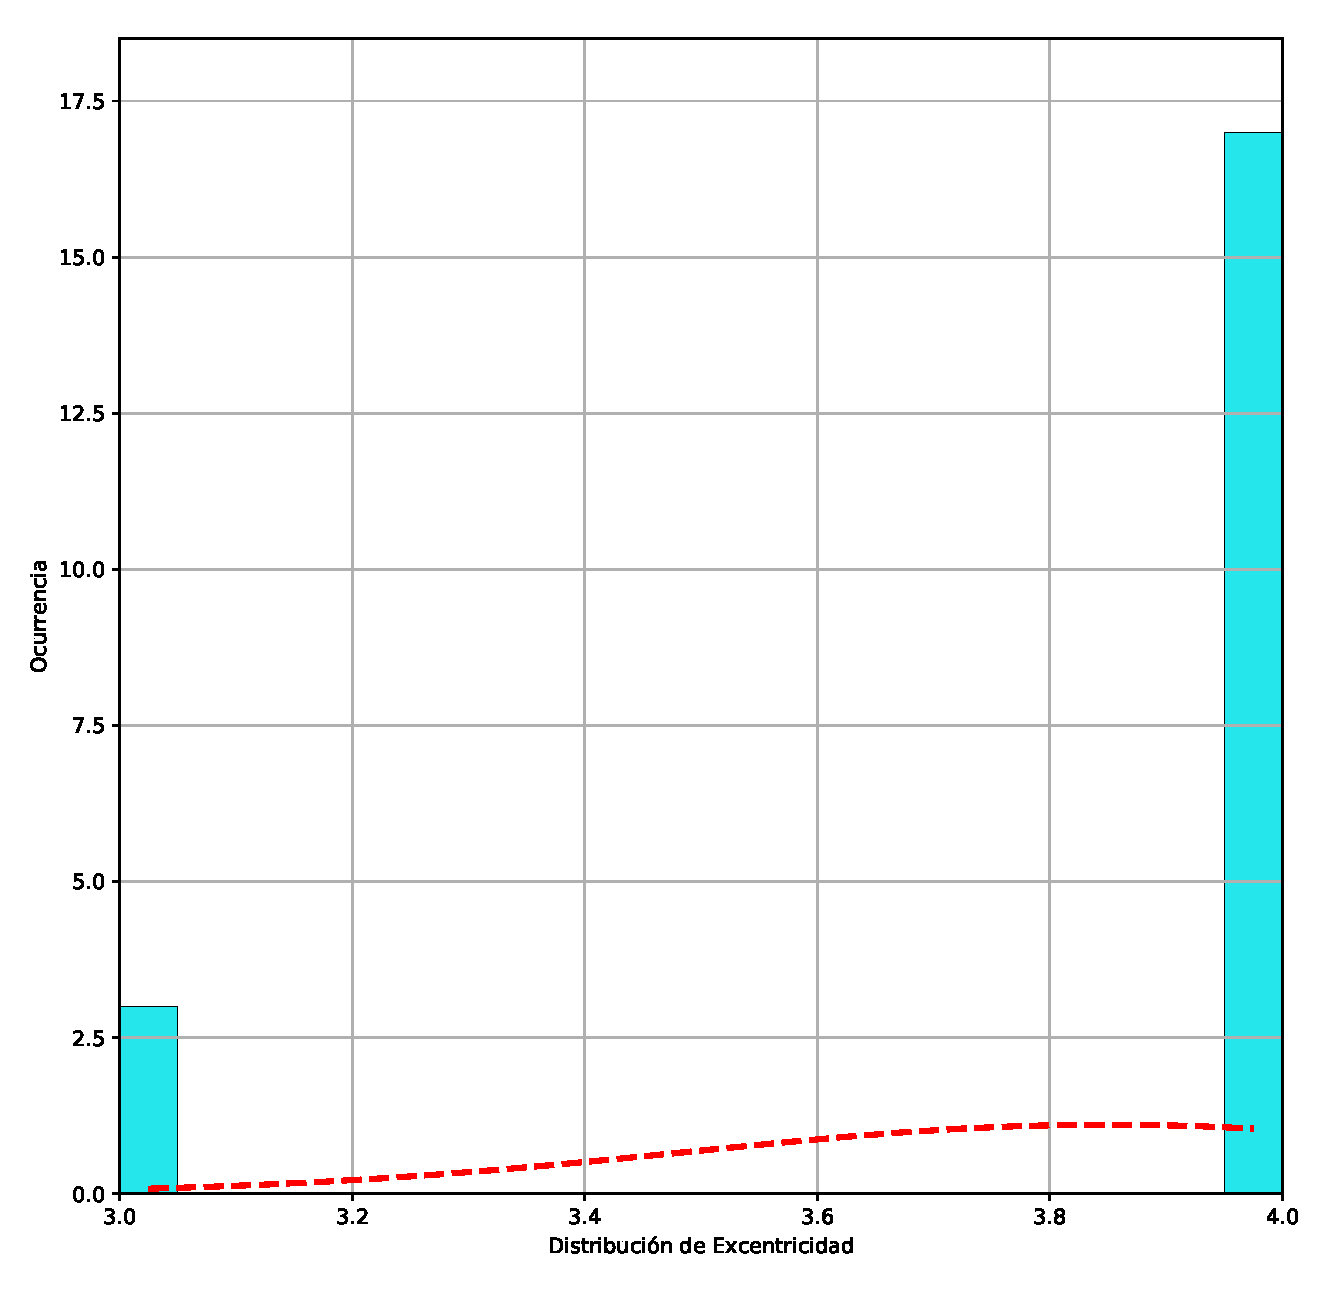
\includegraphics[scale=0.3]{ExcentricidadGrafo1D.eps}}
\subfigure[\textit{Grafo2}]{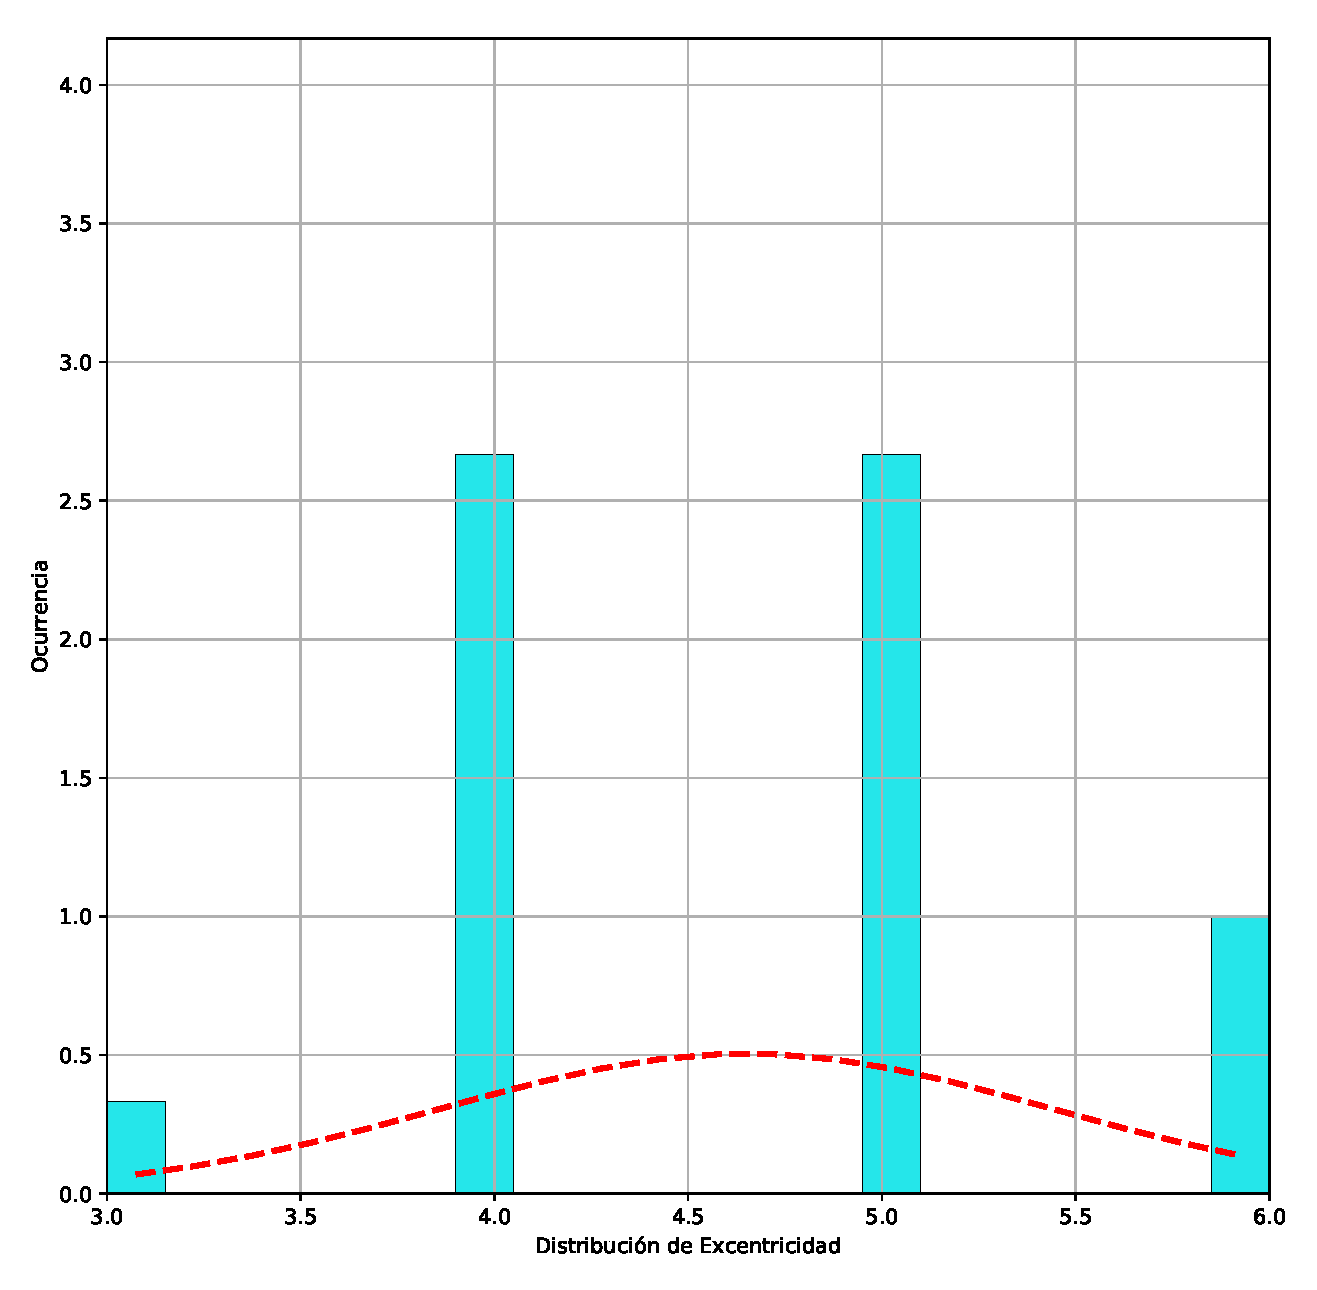
\includegraphics[scale=0.3]{ExcentricidadGrafo2D.eps}}
\subfigure[\textit{Grafo3}]{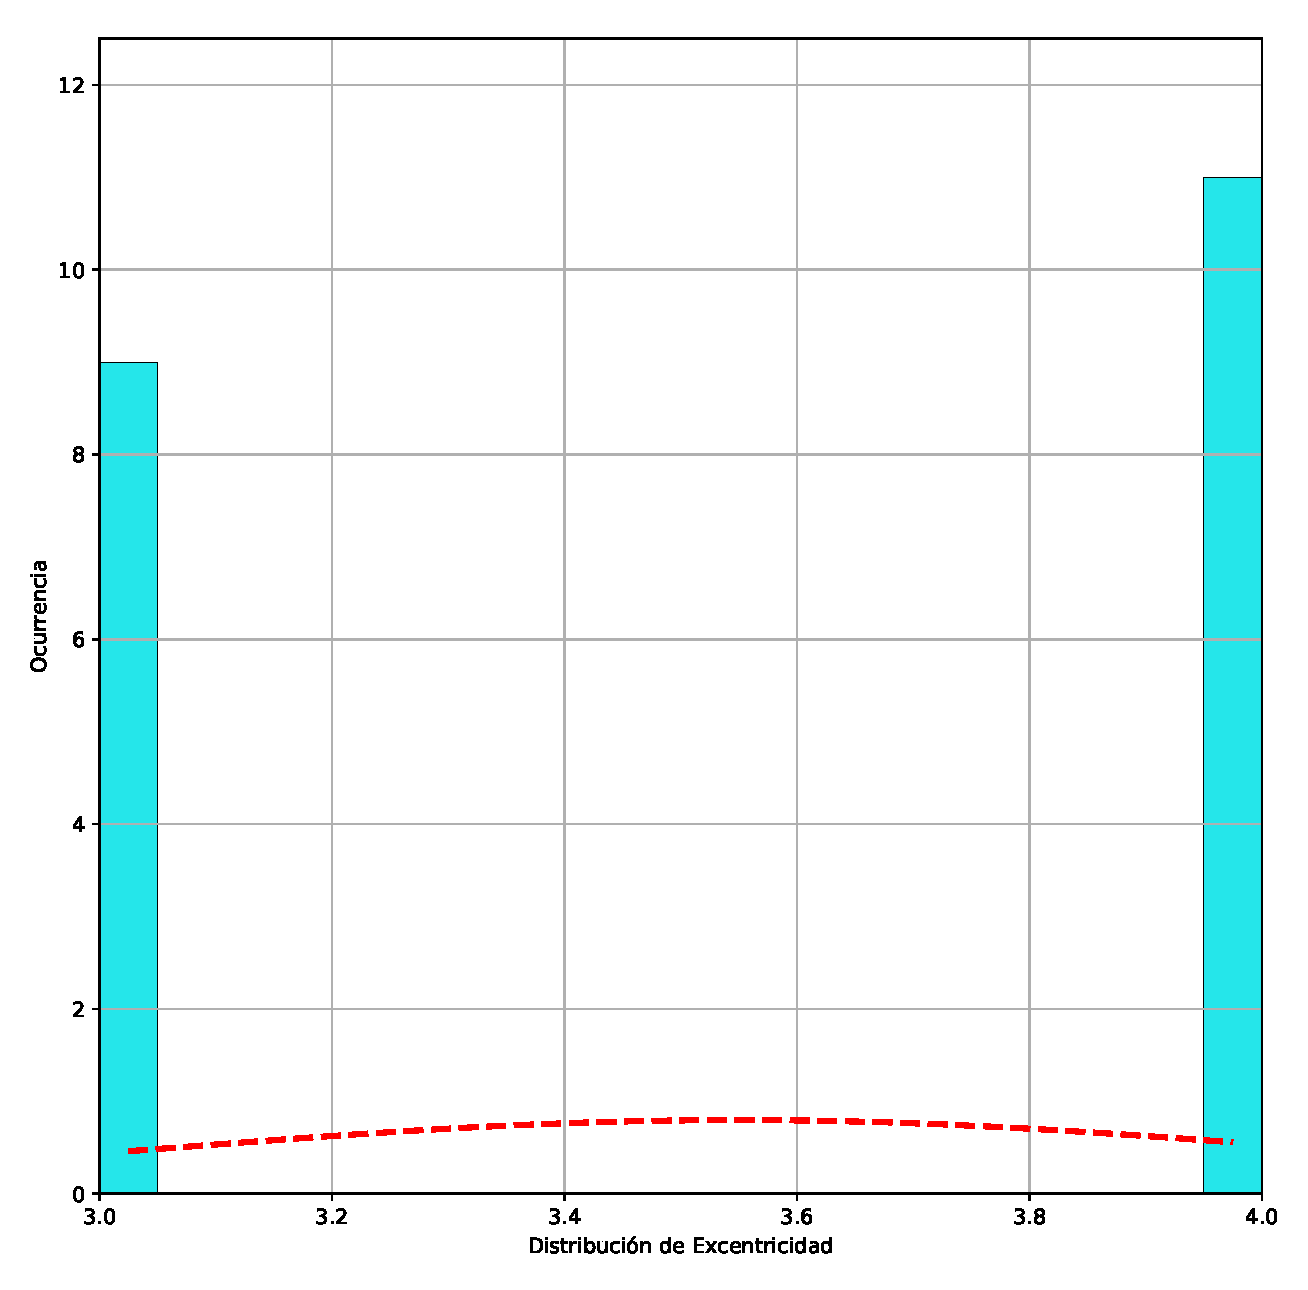
\includegraphics[scale=0.3]{ExcentricidadGrafo3D.eps}}
\subfigure[\textit{Grafo4}]{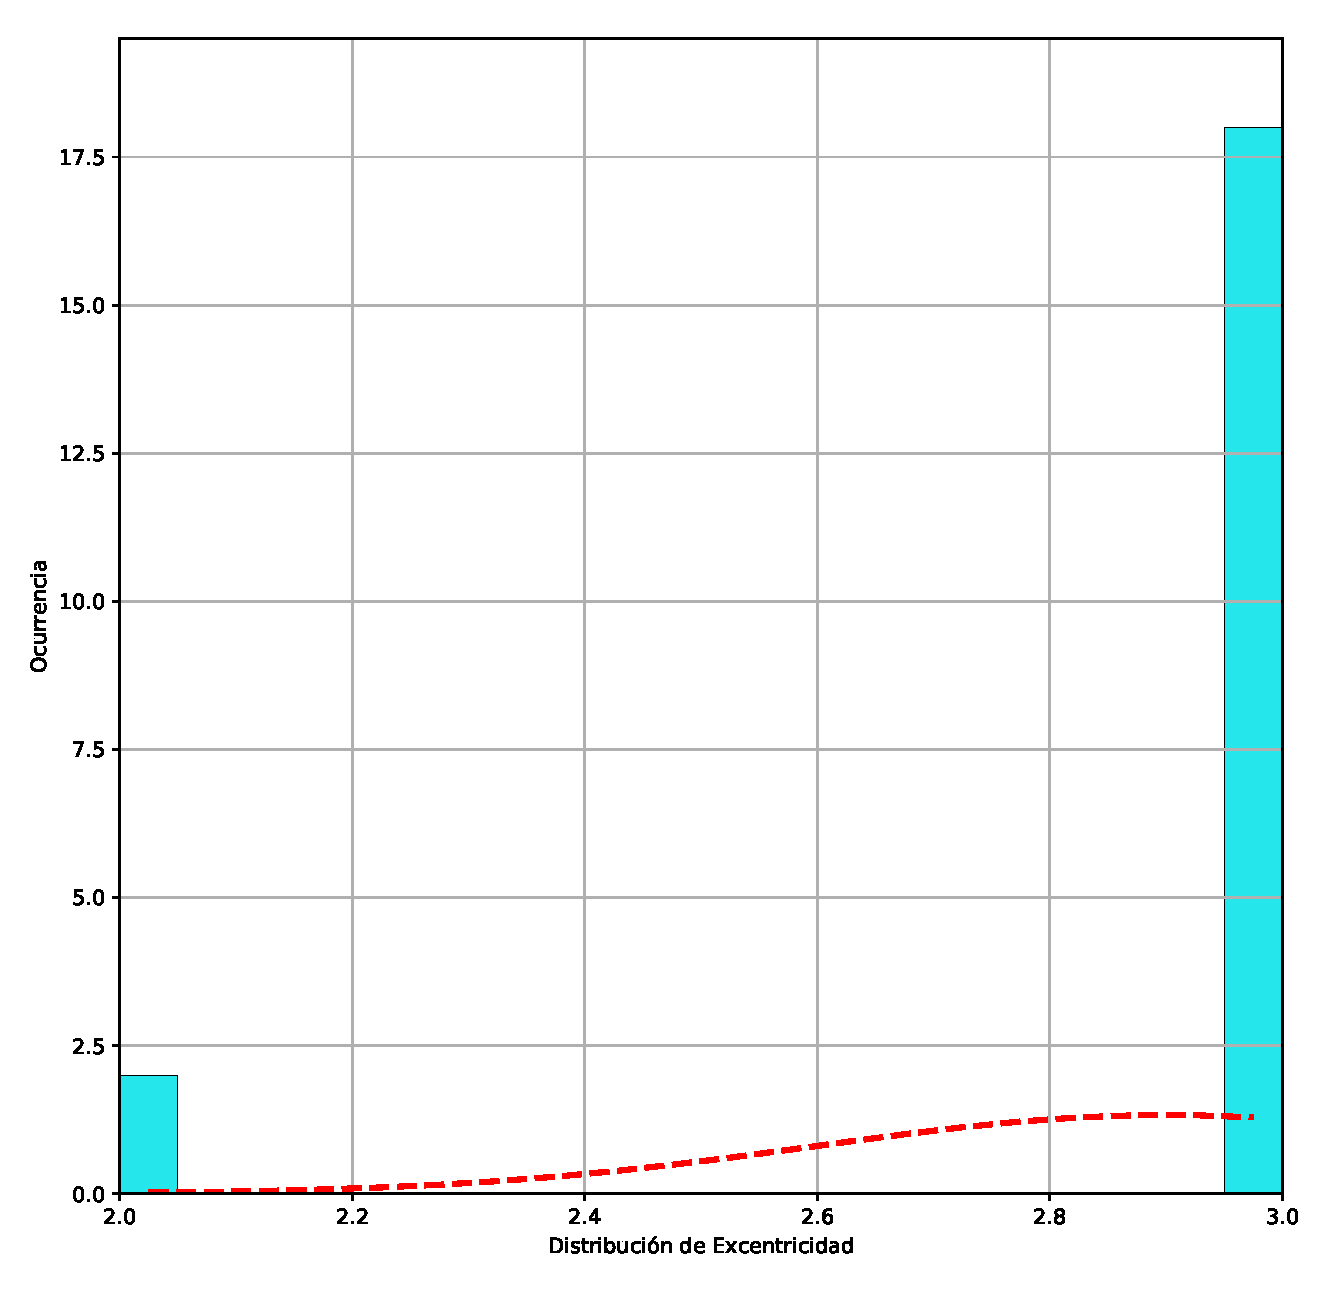
\includegraphics[scale=0.3]{ExcentricidadGrafo4D.eps}}
\subfigure[\textit{Grafo5}]{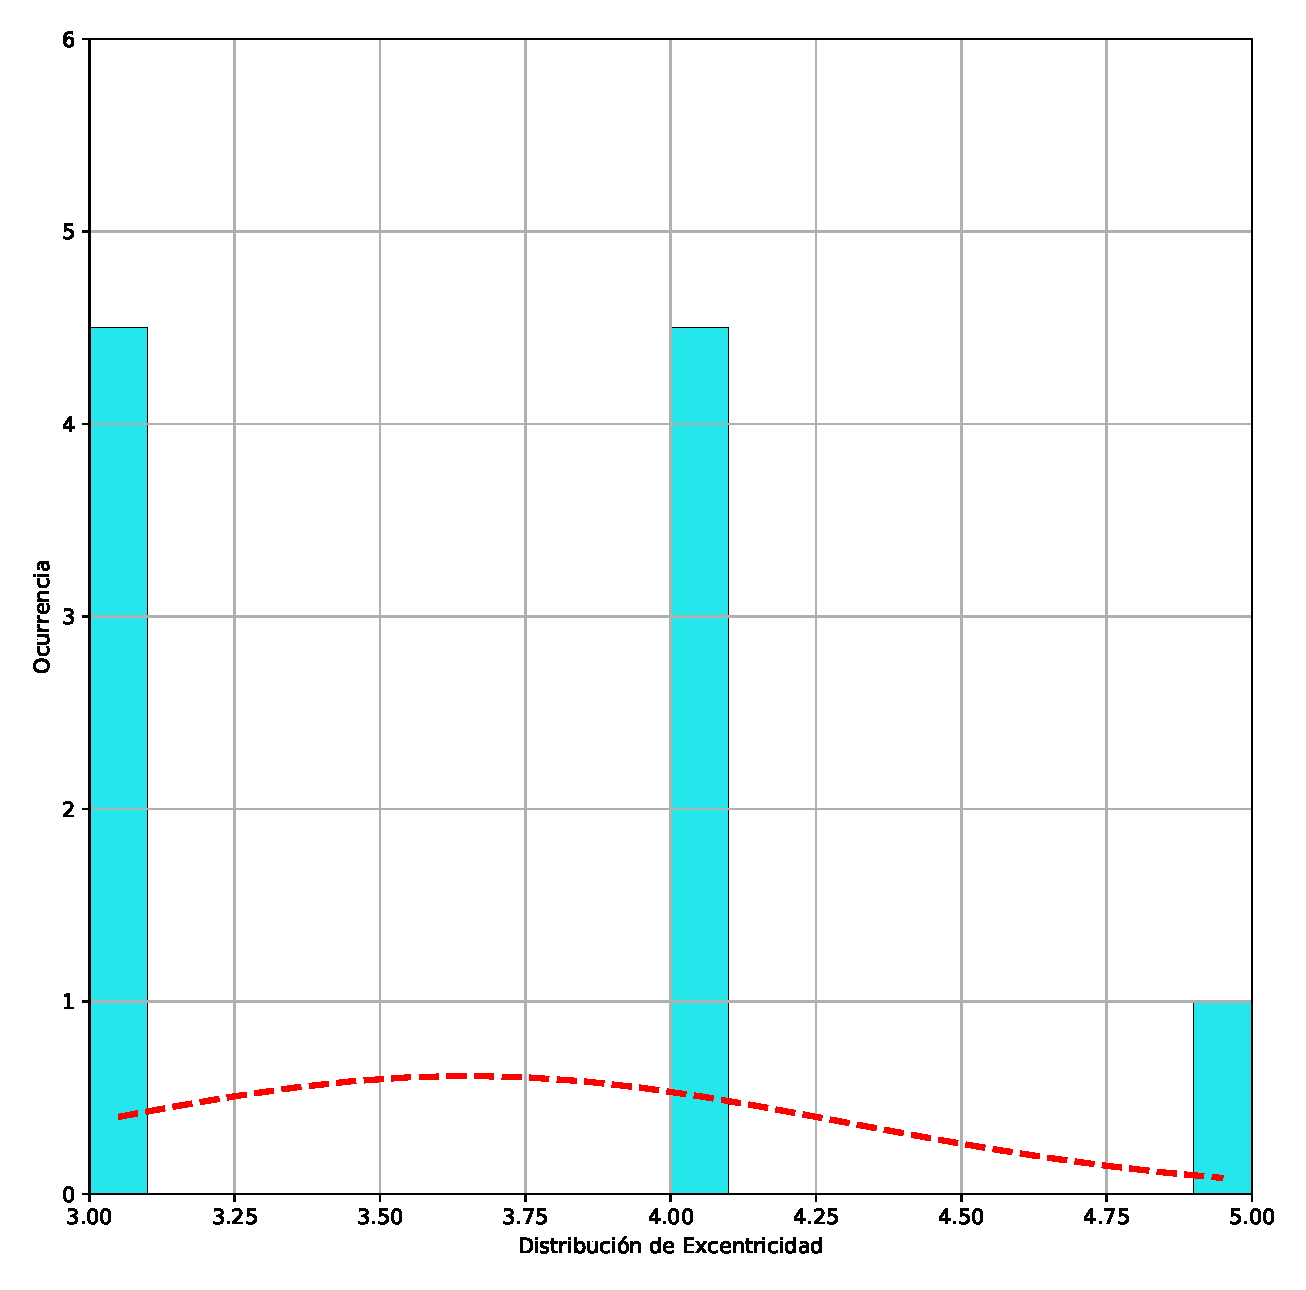
\includegraphics[scale=0.3]{ExcentricidadGrafo5D.eps}}

\caption{Histogramas que muestran la distribución de los valores de la característica excentricidad. }
\label{fig11} 
\end{figure}

\begin{figure}[htbp]

\subfigure[\textit{Grafo1}]{\includegraphics[scale=0.3]{PageRagGrafo1D.eps}}
\subfigure[\textit{Grafo2}]{\includegraphics[scale=0.3]{PageRagGrafo2D.eps}}
\subfigure[\textit{Grafo3}]{\includegraphics[scale=0.3]{PageRagGrafo3D.eps}}
\subfigure[\textit{Grafo4}]{\includegraphics[scale=0.3]{PageRagGrafo4D.eps}}
\subfigure[\textit{Grafo5}]{\includegraphics[scale=0.3]{PageRagGrafo5D.eps}}

\caption{Histogramas que muestran la distribución de los valores de la característica \textit{PageRank}. }
\label{fig12} 
\end{figure}
Dado que la distribución de los valores de las características no es normal, se hizo una categorización por rangos para hacer cómoda la visualización de la relación con las variables dependientes, estos rangos se obtuvieron a través de los contenedores que devolvió histogramas que se le aplicaron a cada propiedad.

Con esta categorización de las características se realizaron las pruebas estadísticas para analizar la in fluencia de las características estructurales de los grafos en el tiempo de ejecución del algoritmo de flujo máximo y el valor de flujo máximo.

El siguiente fragmento de código nos muestra la realización de las pruebas antes mencionadas.

 
\begin{center}
\lstinputlisting[language=Python, firstline=90, lastline=127]{Analisis_datos1.py}
\end{center}
\subsection{Análisis de varianza (ANOVA)}
El análisis de varianza (ANOVA) es la técnica central en el análisis de datos experimentales. La idea general de esta técnica es separar la variación total en las partes con las que contribuye cada fuente de variación en el experimento. En el caso de los diseños completamente al azar se separan la variabilidad debida a los tratamientos y la debida al error. Cuando la primera predomina sobre la segunda, es cuando se concluye que las medias son diferentes. Cuando los tratamientos no dominan contribuyen igual o menos que el error, por lo que se concluye que las medias son iguales \cite{ade}.
%
Para analizar si los diferentes factores (distribución de grado, coeficiente de agrupamiento, centralidad de cercanía, centralidad de carga, excentricidad, \textit{pagerank}) influyen en lsa variable dependiente \textit{tiempo de ejecución} y valores de flujo máximo se realizó un ANOVA de un factor para cada caso. 

\subsubsection{Influencia de la distribución de grado en el tiempo de ejecución}
El siguiente cuadro muestra el resultado de la aplicación del ANOVA.
% Table generated by Excel2LaTeX from sheet 'ANOVAsFlujoMaxGrado'
\begin{table}[htbp]
  \centering
  \caption{Influencia de la distribución de grado en el tiempo de ejecución (ANOVA)}
    \begin{tabular}{lrrrlll}
    \toprule
    \textit{\textbf{Source}} & \multicolumn{1}{l}{\textit{\textbf{SS}}} & \multicolumn{1}{l}{\textit{\textbf{DF}}} & \multicolumn{1}{l}{\textit{\textbf{MS}}} & \textit{\textbf{F}} & \textit{\textbf{p-unc}} & \textit{\textbf{np2}} \\
    \midrule
    \textit{Grado} & 209597.452 & 2.000 & 104798.726 & \multicolumn{1}{r}{662.186} & \multicolumn{1}{r}{0.000} & \multicolumn{1}{r}{0.411} \\
    \textit{Within} & 300222.666 & 1897.000 & 158.262 & -     & -     & - \\
    \bottomrule
    \end{tabular}%
  \label{tab:tab3}%
\end{table}%

En el cuadro \ref{tab:tab3} se muestra que existen diferencia entre las medianas de los grupos de factores ya que el \textbf{$p-unc$} es menor que $0.05$ por lo que se rechaza la hipótesis de que la distribución de grado no influye en el \textit{tiempo de ejecución}. Esto se puede observar en la figura \ref{fig13} de la página \pageref{fig13}. 

\begin{center}
\begin{figure}[htbp]
\includegraphics[scale=0.6]{boxplot_Grado.eps}
\caption{Diagrama de caja y bigotes que relaciona los tiempos de ejecución con la distribución de grado.}
\label{fig13}
\end{figure}
\end{center}

En el cuadro \ref{tab:tab3} se muestra que existen grandes diferencia entre las medianas de los grupos de factores ya que el \textbf{$p-unc$} es menor que $0.05$ por lo que se se rechaza la hipótesis de que la distribución de grado no influye en el \textit{tiempo de ejecución}. Esto se puede observar en la figura \ref{fig4} de la página \pageref{fig4}. Por tal motivo se realiza la prueva de Tukey mostrara las diferencias entre las medianas de los factores, lo que se evidencia en el cuadro \ref{tab:t4} de la página \pageref{tab:t4}.
% Table generated by Excel2LaTeX from sheet 'TukeyGrado'
\begin{table}[htbp]
  \centering
  \caption{Influencia de la distribución de grado en el tiempo de ejecución \textit{(Tukey)}}
    \begin{tabular}{llrrrl}
    \toprule
    \textit{\textbf{group1}} & \textit{\textbf{group2}} & \multicolumn{1}{l}{\textit{\textbf{meandiff}}} & \multicolumn{1}{l}{\textit{\textbf{lower}}} & \multicolumn{1}{l}{\textit{\textbf{upper}}} & \textit{\textbf{reject}} \\
    \midrule
    alta  & baja  & -0.020 & -0.024 & -0.016 & True \\
    alta  & media & -0.011 & -0.015 & -0.007 & True \\
    baja  & media & 0.009 & 0.007 & 0.011 & True \\
    \bottomrule
    \end{tabular}%
  \label{tab:t4}%
\end{table}%

\subsubsection{Influencia del coeficiente de agrupamiento en el tiempo de ejecución}
El siguiente cuadro muestra el resultado de la aplicación del ANOVA.

% Table generated by Excel2LaTeX from sheet 'ANOVAsCoefAg'
\begin{table}[htbp]
  \centering
  \caption{Influencia del coeficiente de agrupamiento en el tiempo de ejecución (ANOVA)}
    \begin{tabular}{lrrrrrr}
    \toprule
    \textit{\textbf{Source}} & \multicolumn{1}{l}{\textit{\textbf{SS}}} & \multicolumn{1}{l}{\textit{\textbf{DF}}} & \multicolumn{1}{l}{\textit{\textbf{MS}}} & \multicolumn{1}{l}{\textit{\textbf{F}}} & \multicolumn{1}{l}{\textit{\textbf{p-unc}}} & \multicolumn{1}{l}{\textit{\textbf{np2}}} \\
    \midrule
    \textit{CoefAg} & 0.013 & 2.000 & 0.006 & 19.962 & 0.000 & 0.021 \\
    \textit{Within} & 0.610 & 1897.000 & 0.000 &       &       &  \\
    \bottomrule
    \end{tabular}%
  \label{tab:t5}%
\end{table}%

En el cuadro \ref{tab:t5} se muestra que existen diferencia entre las medianas de los grupos de factores ya que el \emph{$p-unc$} es menor que $0.05$ por lo que se rechaza la hipótesis de que el coeficiente de agrupamiento no influye en el \textit{tiempo de ejecución}. Esto se puede observar en la figura \ref{fig14} de la página \pageref{fig14}. 

\begin{center}
\begin{figure}[htbp]
\includegraphics[scale=0.6]{boxplot_CentCer.eps}
\caption{Diagrama de caja y bigotes que relaciona los tiempos de ejecución con el coeficiente de agrupamiento.}
\label{fig14}
\end{figure}
\end{center}

En el cuadro \ref{tab:t5} se muestra que existen marcadas diferencia entre las medianas de dos de los grupos de factores \textbf{$p-unc$} es menor que $0.05$ por lo que se se rechaza la hipótesis de que el coeficiente de agrupamiento no influye en el \textit{tiempo de ejecución}. Esto se puede observar en la figura \ref{fig14} de la página \pageref{fig14}. Por tal motivo se realiza la prueva de Tukey mostrara las diferencias entre las medianas de los factores, lo que se evidencia en el cuadro \ref{tab:t6} de la página \pageref{tab:t6}.

% Table generated by Excel2LaTeX from sheet 'TukeyCoefAg'
\begin{table}[htbp]
  \centering
  \caption{Influencia del coeficiente de agrupamiento en el tiempo de ejecución (Tukey)}
    \begin{tabular}{llrrrl}
    \toprule
    \textit{\textbf{group1}} & \textit{\textbf{group2}} & \multicolumn{1}{l}{\textit{\textbf{meandiff}}} & \multicolumn{1}{l}{\textit{\textbf{lower}}} & \multicolumn{1}{l}{\textit{\textbf{upper}}} & \textit{\textbf{reject}} \\
    \midrule
    alta  & baja  & 0.005 & -0.001 & 0.010 & False \\
    alta  & media & 0.014 & 0.007 & 0.020 & True \\
    baja  & media & 0.009 & 0.005 & 0.013 & True \\
    \bottomrule
    \end{tabular}%
  \label{tab:t6}%
\end{table}%


\subsubsection{Influencia de la centralidad de cercanía en el tiempo de ejecución}

El siguiente cuadro muestra el resultado de la aplicación del ANOVA.

% Table generated by Excel2LaTeX from sheet 'ANOVAsCentCer'
\begin{table}[htbp]
  \centering
  \caption{Influencia de la centralidad de cercanía en el tiempo de ejecución}
    \begin{tabular}{lrrrrrr}
    \toprule
    \textit{\textbf{Source}} & \multicolumn{1}{l}{\textit{\textbf{SS}}} & \multicolumn{1}{l}{\textit{\textbf{DF}}} & \multicolumn{1}{l}{\textit{\textbf{MS}}} & \multicolumn{1}{l}{\textit{\textbf{F}}} & \multicolumn{1}{l}{\textit{\textbf{p-unc}}} & \multicolumn{1}{l}{\textit{\textbf{np2}}} \\
    \midrule
    \textit{CentCer} & 0.054 & 2.000 & 0.027 & 89.249 & 0.000 & 0.086 \\
    \textit{Within} & 0.570 & 1897.000 & 0.000 &       &       &  \\
    \bottomrule
    \end{tabular}%
  \label{tab:t7}%
\end{table}%

En el cuadro \ref{tab:t7} se muestra que existen diferencia entre las medianas de los grupos de factores ya que el \emph{$p-unc$} es menor que $0.05$ por lo que se rechaza la hipótesis de que la centralidad de cercanía no influye en el \textit{tiempo de ejecución}. Esto se puede observar en la figura \ref{fig15} de la página \pageref{fig15}.

 \begin{center}
\begin{figure}[htbp]
\includegraphics[scale=0.6]{boxplot_CoefAg.eps}
\caption{Diagrama de caja y bigotes que relaciona los tiempos de ejecución con la centralidad de cercanía.}
\label{fig15}
\end{figure}
\end{center}

En el cuadro \ref{tab:t7} se muestra que existen marcadas diferencia entre las medianas de dos de los grupos de factores  \textbf{$p-unc$} es menor que $0.05$ por lo que se se rechaza la hipótesis de que la centralidad de cercanía no influye en el \textit{tiempo de ejecución}. Esto se puede observar en la figura \ref{fig15} de la página \pageref{fig15}. Por tal motivo se realiza la prueva de Tukey mostrara las diferencias entre las medianas de los factores, lo que se evidencia en el cuadro \ref{tab:t8} de la página \pageref{tab:t8}.
% Table generated by Excel2LaTeX from sheet 'TukeyCentCer'
\begin{table}[htbp]
  \centering
  \caption{Influencia de la centralidad de cercanía en el tiempo de ejecución (Tukey)}
    \begin{tabular}{llrrrl}
    \toprule
    \textit{\textbf{group1}} & \textit{\textbf{group2}} & \multicolumn{1}{l}{\textit{\textbf{meandiff}}} & \multicolumn{1}{l}{\textit{\textbf{lower}}} & \multicolumn{1}{l}{\textit{\textbf{upper}}} & \textit{\textbf{reject}} \\
    \midrule
    alta  & baja  & -0.016 & -0.018 & -0.013 & \textit{True} \\
    alta  & media & -0.008 & -0.011 & -0.006 & \textit{True} \\
    baja  & media & 0.007 & 0.005 & 0.010 & \textit{True} \\
    \bottomrule
    \end{tabular}%
  \label{tab:t8}%
\end{table}%


\subsubsection{Influencia de la centralidad de carga en el tiempo de ejecución}

El siguiente cuadro muestra el resultado de la aplicación del ANOVA.

% Table generated by Excel2LaTeX from sheet 'ANOVAsCentCag'
\begin{table}[htbp]
  \centering
  \caption{Influencia de la centralidad de carga en el tiempo de ejecución (ANOVA)}
    \begin{tabular}{lrrrrrr}
    \toprule
    \textit{\textbf{Source}} & \multicolumn{1}{l}{\textit{\textbf{SS}}} & \multicolumn{1}{l}{\textit{\textbf{DF}}} & \multicolumn{1}{l}{\textit{\textbf{MS}}} & \multicolumn{1}{l}{\textit{\textbf{F}}} & \multicolumn{1}{l}{\textit{\textbf{p-unc}}} & \multicolumn{1}{l}{\textit{\textbf{np2}}} \\
    \midrule
    \textit{CentCag} & 0.000 & 2.000 & 0.000 & 0.476 & 0.621 & 0.001 \\
    \textit{Within} & 0.623 & 1897.000 & 0.000 &       &       &  \\
    \bottomrule
    \end{tabular}%
  \label{tab:t9}%
\end{table}%

En el cuadro \ref{tab:t9} se muestra que no existen diferencia entre las medianas de los grupos de factores ya que el \emph{$p-unc$} es meyor que $0.05$ por lo que se acepta la hipótesis de que la centralidad de carga no influye en el \textit{tiempo de ejecución}. Esto se puede observar en la figura \ref{fig16} de la página \pageref{fig16}.

\begin{center}
\begin{figure}[htbp]
\includegraphics[scale=0.6]{boxplot_CentCag.eps}
\caption{Diagrama de caja y bigotes que relaciona los tiempos de ejecución con la centralidad de carga.}
\label{fig16}
\end{figure}
\end{center}

\subsubsection{Influencia de la excentricidad en el tiempo de ejecución}
El siguiente cuadro muestra el resultado de la aplicación del ANOVA.

% Table generated by Excel2LaTeX from sheet 'ANOVAsExcentricidad'
\begin{table}[htbp]
  \centering
  \caption{Influencia de la excentricidad en el tiempo de ejecución (ANOVA)}
    \begin{tabular}{lrrrrrr}
    \toprule
    \textit{\textbf{Source}} & \multicolumn{1}{l}{\textit{\textbf{SS}}} & \multicolumn{1}{l}{\textit{\textbf{DF}}} & \multicolumn{1}{l}{\textit{\textbf{MS}}} & \multicolumn{1}{l}{\textit{\textbf{F}}} & \multicolumn{1}{l}{\textit{\textbf{p-unc}}} & \multicolumn{1}{l}{\textit{\textbf{np2}}} \\
    \midrule
    \textit{Excentricidad} & 0.043 & 2.000 & 0.021 & 70.117 & 0.000 & 0.069 \\
    \textit{Within} & 0.580 & 1897.000 & 0.000 &       &       &  \\
    \bottomrule
    \end{tabular}%
  \label{tab:t10}%
\end{table}%

En el cuadro \ref{tab:t10} se muestra que existen diferencia entre las medianas de los grupos de factores ya que el \emph{$p-unc$} es menor que $0.05$ por lo que se rechaza la hipótesis de que la excentricidad no influye en el \textit{tiempo de ejecución}. Esto se puede observar en la figura \ref{fig17} de la página \pageref{fig17}.

\begin{center}
\begin{figure}[htbp]
\includegraphics[scale=0.6]{boxplot_Excentricidad.eps}
\caption{Diagrama de caja y bigotes que relaciona los tiempos de ejecución con la excentricidad.}
\label{fig17}
\end{figure}
\end{center}

En el cuadro \ref{tab:t10} se muestra que existen  diferencia entre las medianas de dos de los grupos de factores  \textbf{$p-unc$} es menor que $0.05$ por lo que se se rechaza la hipótesis de que la excentricidad no influye en el \textit{tiempo de ejecución}. Esto se puede observar en la figura \ref{fig17} de la página \pageref{fig17}. Por tal motivo se realiza la prueva de Tukey mostrara las diferencias entre las medianas de los factores, lo que se evidencia en el cuadro \ref{tab:t11} de la página \pageref{tab:t11}.

% Table generated by Excel2LaTeX from sheet 'TukeyExcentricidad'
\begin{table}[htbp]
  \centering
  \caption{Influencia de la excentricidad en el tiempo de ejecución (Tukey)}
    \begin{tabular}{llrrrl}
    \toprule
    \textbf{group1} & \textbf{group2} & \multicolumn{1}{l}{\textit{\textbf{meandiff}}} & \multicolumn{1}{l}{\textit{\textbf{lower}}} & \multicolumn{1}{l}{\textit{\textbf{upper}}} & \textit{\textbf{reject}} \\
    \midrule
    alta  & baja  & 0.013 & 0.010 & 0.016 & \textit{True} \\
    alta  & media & 0.004 & 0.001 & 0.007 & \textit{True} \\
    baja  & media & -0.008 & -0.010 & -0.006 & \textit{True} \\
    \bottomrule
    \end{tabular}%
  \label{tab:t11}%
\end{table}%

\subsubsection{Influencia del \textit{PageRank} en el tiempo de ejecución}

El siguiente cuadro muestra el resultado de la aplicación del ANOVA.

% Table generated by Excel2LaTeX from sheet 'ANOVAsPageRag'
\begin{table}[htbp]
  \centering
  \caption{Influencia del \textit{PageRank} en el tiempo de ejecución (ANOVA)}
    \begin{tabular}{lrrrrrr}
    \toprule
    \textit{\textbf{Source}} & \multicolumn{1}{l}{\textit{\textbf{SS}}} & \multicolumn{1}{l}{\textit{\textbf{DF}}} & \multicolumn{1}{l}{\textit{\textbf{MS}}} & \multicolumn{1}{l}{\textit{\textbf{F}}} & \multicolumn{1}{l}{\textit{\textbf{p-unc}}} & \multicolumn{1}{l}{\textit{\textbf{np2}}} \\
    \midrule
    \textit{PageRag} & 0.016 & 2.000 & 0.008 & 25.358 & 0.000 & 0.026 \\
    \textit{Within} & 0.607 & 1897.000 & 0.000 &       &       &  \\
    \bottomrule
    \end{tabular}%
  \label{tab:t12}%
\end{table}%

En el cuadro \ref{tab:t12} se muestra que existen diferencia entre las medianas de los grupos de factores ya que el \emph{$p-unc$} es menor que $0.05$ por lo que se rechaza la hipótesis de que el \textit{PageRank} no influye en el \textit{tiempo de ejecución}. Esto se puede observar en la figura \ref{fig18} de la página \pageref{fig18}

\begin{center}
\begin{figure}[htbp]
\includegraphics[scale=0.6]{boxplot_PageRag.eps}
\caption{Diagrama de caja y bigotes que relaciona los tiempos de ejecución con el \textit{PageRank}.}
\label{fig18}
\end{figure}
\end{center}


En el cuadro \ref{tab:t12} se muestra que existen  diferencia entre las medianas de dos de los grupos de factores  \textbf{$p-unc$} es menor que $0.05$ por lo que se se rechaza la hipótesis de que el \textit{PageRank} no influye en el \textit{tiempo de ejecución}. Esto se puede observar en la figura \ref{fig17} de la página \pageref{fig17}. Por tal motivo se realiza la prueva de Tukey mostrara las diferencias entre las medianas de los factores, lo que se evidencia en el cuadro \ref{tab:t19} de la página \pageref{tab:t19}.

% Table generated by Excel2LaTeX from sheet 'TukeyPageRag'
\begin{table}[htbp]
  \centering
  \caption{Influencia del \textit{PageRank} en el tiempo de ejecuciónAdd (Tukey)}
    \begin{tabular}{llrrrl}
    \textit{\textbf{group1}} & \textit{\textbf{group2}} & \multicolumn{1}{l}{\textit{\textbf{meandiff}}} & \multicolumn{1}{l}{\textit{\textbf{lower}}} & \multicolumn{1}{l}{\textit{\textbf{upper}}} & \textit{\textbf{reject}} \\
    alta  & baja  & -0.001 & -0.006 & 0.005 & \textit{False} \\
    alta  & media & 0.005 & -0.001 & 0.011 & \textit{False} \\
    baja  & media & 0.006 & 0.004 & 0.008 & \textit{True} \\
    \end{tabular}%
  \label{tab:t19}%
\end{table}%

\subsubsection{Influencia de los seis factores (distribución de grado, coeficiente de agrupamiento, centralidad de cercanía, centralidad de carga, excentricidad, \textit{pagerank}) en el tiempo de ejecución}
Para analizar este caso se realizo ANOVA multifactorial dando como resultado el cuadro \ref{tab:t20} de la página \pageref{tab:t20}.

% Table generated by Excel2LaTeX from sheet 'modelo'
\begin{table}[htbp]
  \centering
  \caption{Influencia de los seis factores (distribución de grado, coeficiente de agrupamiento, centralidad de cercanía, centralidad de carga, excentricidad, \textit{pagerank}) en el tiempo de ejecución (MANOVA)}
    \begin{tabular}{lrrrr}
          & \multicolumn{1}{l}{\textit{\textbf{sum\_sq}}} & \multicolumn{1}{l}{\textit{\textbf{df}}} & \multicolumn{1}{l}{\textit{\textbf{F}}} & \multicolumn{1}{l}{\textit{\textbf{\texttt{PR(>F)}}}} \\
    Grado & 0.000 & 2.000 & 0.000 & 1.000 \\
    CoefAg & 0.000 & 2.000 & 0.000 & 1.000 \\
    CentCer & 0.000 & 2.000 & -0.409 & 1.000 \\
    CentCag & 0.000 & 2.000 & 0.000 & 1.000 \\
    Excentricidad & 0.000 & 2.000 & 0.000 & 1.000 \\
    PageRag & 0.000 & 2.000 & 0.000 & 1.000 \\
    Grado:CoefAg & 0.001 & 4.000 & 0.594 & 0.619 \\
    Grado:CentCer & 0.001 & 4.000 & 1.048 & 0.381 \\
    Grado:CentCag & 0.001 & 4.000 & 0.854 & 0.491 \\
    Grado:Excentricidad & 0.001 & 4.000 & 1.064 & 0.373 \\
    Grado:PageRag & 0.001 & 4.000 & 0.858 & 0.489 \\
    CoefAg:CentCer & 0.001 & 4.000 & 0.560 & 0.571 \\
    CoefAg:CentCag & 0.001 & 4.000 & 0.525 & 0.665 \\
    CoefAg:Excentricidad & 0.000 & 4.000 & 0.203 & 0.816 \\
    CoefAg:PageRag & 0.001 & 4.000 & 0.430 & 0.731 \\
    CentCer:CentCag & 0.001 & 4.000 & 0.758 & 0.517 \\
    CentCer:Excentricidad & 0.001 & 4.000 & 0.543 & 0.653 \\
    CentCer:PageRag & 0.001 & 4.000 & 0.755 & 0.519 \\
    CentCag:Excentricidad & 0.001 & 4.000 & 0.584 & 0.626 \\
    CentCag:PageRag & 0.001 & 4.000 & 0.640 & 0.527 \\
    Excentricidad:PageRag & 0.001 & 4.000 & 0.677 & 0.608 \\
    Residual & 0.549 & 1876.000 &       &  \\
    \end{tabular}%
  \label{tab:t20}%
\end{table}%

En el cuadro \ref{tab:t7} se puede observar que los factores que más influyen en el tiempo de ejecución son el número de vértices y la densidad de los grafos, que además existe una relación entre el número de nodos y la densidad de los grafos.

\subsubsection{Influencia de las seis propiedades en el flujo máximo}

Los cuadro \ref{tab:t21}, \ref{tab:t22}, \ref{tab:t23}, \ref{tab:t24}, \ref{tab:t25}, \ref{tab:t25} de las páginas \pageref{tab:t21}, \pageref{tab:t22}, \pageref{tab:t23}, \pageref{tab:t24},\pageref{tab:t25}, \pageref{tab:t26} respectivamente, muestran los resultados de la aplicación del ANOVA en las  seis propiedades con respecto los valores de flujo máximo.


% Table generated by Excel2LaTeX from sheet 'ANOVAsFlujoMaxGrado'
\begin{table}[htbp]
  \centering
  \caption{Influencia de la distribución de grado en el flujo máximo (ANOVA)}
    \begin{tabular}{lrrrrrr}
    \toprule
    \textit{\textbf{Source}} & \multicolumn{1}{l}{\textit{\textbf{SS}}} & \multicolumn{1}{l}{\textit{\textbf{DF}}} & \multicolumn{1}{l}{\textit{\textbf{MS}}} & \multicolumn{1}{l}{\textit{\textbf{F}}} & \multicolumn{1}{l}{\textit{\textbf{p-unc}}} & \multicolumn{1}{l}{\textit{\textbf{np2}}} \\
    \midrule
    \textit{Grado} & 209597.452 & 2.000 & 104798.726 & 662.186 & 0.000 & 0.411 \\
    \textit{Within} & 300222.666 & 1897.000 & 158.262 &       &       &  \\
    \bottomrule
    \end{tabular}%
  \label{tab:t21}%
\end{table}%

% Table generated by Excel2LaTeX from sheet 'ANOVAsFlujoMaxCoefAg'
\begin{table}[htbp]
  \centering
  \caption{Influencia de la distribución de coeficiente de agrupamiento en el flujo máximo (ANOVA)}
    \begin{tabular}{lrrrrrr}
    \toprule
    \textit{\textbf{Source}} & \multicolumn{1}{l}{\textit{\textbf{SS}}} & \multicolumn{1}{l}{\textit{\textbf{DF}}} & \multicolumn{1}{l}{\textit{\textbf{MS}}} & \multicolumn{1}{l}{\textit{\textbf{F}}} & \multicolumn{1}{l}{\textit{\textbf{p-unc}}} & \multicolumn{1}{l}{\textit{\textbf{np2}}} \\
    \midrule
    \textit{CoefAg} & 59963.814 & 2.000 & 29981.907 & 126.431 & 0.000 & 0.118 \\
    \textit{Within} & 449856.304 & 1897.000 & 237.141 &       &       &  \\
    \bottomrule
    \end{tabular}%
  \label{tab:t22}%
\end{table}%

% Table generated by Excel2LaTeX from sheet 'ANOVAsFlujoMaxCentCer'
\begin{table}[htbp]
  \centering
  \caption{Influencia de la distribución de centralidad de cercanía en el flujo máximo (ANOVA)}
    \begin{tabular}{lrrrrrr}
    \toprule
    \textit{\textbf{Source}} & \multicolumn{1}{l}{\textit{\textbf{SS}}} & \multicolumn{1}{l}{\textit{\textbf{DF}}} & \multicolumn{1}{l}{\textit{\textbf{MS}}} & \multicolumn{1}{l}{\textit{\textbf{F}}} & \multicolumn{1}{l}{\textit{\textbf{p-unc}}} & \multicolumn{1}{l}{\textit{\textbf{np2}}} \\
    \midrule
    \textit{CentCer} & 256496.045 & 2.000 & 128248.023 & 960.377 & 0.000 & 0.503 \\
    \textit{Within} & 253324.073 & 1897.000 & 133.539 &       &       &  \\
    \bottomrule
    \end{tabular}%
  \label{tab:t23}%
\end{table}%

% Table generated by Excel2LaTeX from sheet 'ANOVAsFlujoMaxCentCag'
\begin{table}[htbp]
  \centering
  \caption{Influencia de la centralidad de carga  en el flujo máximo (ANOVA)}
    \begin{tabular}{lrrrrrr}
    \toprule
    \textit{\textbf{Source}} & \multicolumn{1}{l}{\textit{\textbf{SS}}} & \multicolumn{1}{l}{\textit{\textbf{DF}}} & \multicolumn{1}{l}{\textit{\textbf{MS}}} & \multicolumn{1}{l}{\textit{\textbf{F}}} & \multicolumn{1}{l}{\textit{\textbf{p-unc}}} & \multicolumn{1}{l}{\textit{\textbf{np2}}} \\
    \midrule
    \textit{CentCag} & 6469.019 & 2.000 & 3234.510 & 12.190 & 0.000 & 0.013 \\
    \textit{Within} & 503351.098 & 1897.000 & 265.341 &       &       &  \\
    \bottomrule
    \end{tabular}%
  \label{tab:t24}%
\end{table}%


% Table generated by Excel2LaTeX from sheet 'ANOVAsFlujoMaxExcentricidad'
\begin{table}[htbp]
  \centering
  \caption{Influencia de la excentricidad en el flujo máximo (ANOVA)}
    \begin{tabular}{lrrrlll}
    \toprule
    \textit{\textbf{Source}} & \multicolumn{1}{l}{\textit{\textbf{SS}}} & \multicolumn{1}{l}{\textit{\textbf{DF}}} & \multicolumn{1}{l}{\textit{\textbf{MS}}} & \textit{\textbf{F}} & \textit{\textbf{p-unc}} & \textit{\textbf{np2}} \\
    \midrule
    Excentricidad & 200853.698 & 2.000 & 100426.849 & \multicolumn{1}{r}{616.603} & \multicolumn{1}{r}{0.000} & \multicolumn{1}{r}{0.394} \\
    Within & 308966.420 & 1897.000 & 162.871 & -     & -     & - \\
    \bottomrule
    \end{tabular}%
  \label{tab:t25}%
\end{table}%

% Table generated by Excel2LaTeX from sheet 'ANOVAsFlujoMaxPageRag'
\begin{table}[htbp]
  \centering
  \caption{Influencia de el \textit{pagerank} en el flujo máximo (ANOVA)}
    \begin{tabular}{lrrrrrr}
    \toprule
    \textit{\textbf{Source}} & \multicolumn{1}{l}{\textit{\textbf{SS}}} & \multicolumn{1}{l}{\textit{\textbf{DF}}} & \multicolumn{1}{l}{\textit{\textbf{MS}}} & \multicolumn{1}{l}{\textit{\textbf{F}}} & \multicolumn{1}{l}{\textit{\textbf{p-unc}}} & \multicolumn{1}{l}{\textit{\textbf{np2}}} \\
    \midrule
    \textit{PageRag} & 67070.251 & 2.000 & 33535.125 & 143.684 & 0.000 & 0.132 \\
    \textit{Within} & 442749.867 & 1897.000 & 233.395 &       &       &  \\
    \bottomrule
    \end{tabular}%
  \label{tab:t26}%
\end{table}%

En los cuadro anteriores se muestra que existen diferencia entre las medianas de los grupos de factores ya que el \textbf{$p-unc$} es menor que $0.05$ por lo que se rechaza la hipótesis de que las propiedades no influye en el \textit{flujo máximo}. Esto se puede observar claramente en las figuras \ref{fig19}, \ref{fig20}, \ref{fig21}, \ref{fig22}, \ref{fig23}, \ref{fig23} de las páginas \pageref{fig19}, \pageref{fig20}, \pageref{fig21}, \pageref{fig22}, \pageref{fig23}, \pageref{fig24} respectivamente.


\begin{center}
\begin{figure}[htbp]
\includegraphics[scale=0.6]{boxplot_FlujoMaxGrado.eps}
\caption{Diagrama de caja y bigotes que relaciona los flujos máximos con la distribución de grado.}
\label{fig19}
\end{figure}
\end{center}

\begin{center}
\begin{figure}[htbp]
\includegraphics[scale=0.6]{boxplot_FlujoMaxCoefAg.eps}
\caption{Diagrama de caja y bigotes que relaciona los flujos máximos con el coeficiente de agrupamiento.}
\label{fig20}
\end{figure}
\end{center}

\begin{center}
\begin{figure}[htbp]
\includegraphics[scale=0.6]{boxplot_FlujoMaxCentCer.eps}
\caption{Diagrama de caja y bigotes que relaciona los flujos máximos con la centralidad de cercanía.}
\label{fig21}
\end{figure}
\end{center}

\begin{center}
\begin{figure}[htbp]
\includegraphics[scale=0.6]{boxplot_FlujoMaxCentCag.eps}
\caption{Diagrama de caja y bigotes que relaciona los flujos máximos con la centralidad de carga.}
\label{fig22}
\end{figure}
\end{center}

\begin{center}
\begin{figure}[htbp]
\includegraphics[scale=0.6]{boxplot_FlujoMaxExcentricidad.eps}
\caption{Diagrama de caja y bigotes que relaciona los flujos máximos con la excentricidad.}
\label{fig23}
\end{figure}
\end{center}

\begin{center}
\begin{figure}[htbp]
\includegraphics[scale=0.6]{boxplot_FlujoMaxPageRag.eps}
\caption{Diagrama de caja y bigotes que relaciona los flujos máximos con el  \textit{pagerank}.}
\label{fig24}
\end{figure}
\end{center}
 
Debido a las diferencias obtenidas en todas las ANOVAs realizadas, procedemos a relizar la prueba de Tukey cuyus resultados se muestran el los cuadros 

% Table generated by Excel2LaTeX from sheet 'TukeyFlujoMaxGrado'
\begin{table}[htbp]
  \centering
  \caption{Influencia de la distribución de grado en el flujo máximo (Tukey)}
    \begin{tabular}{llrrrl}
    \toprule
    \textit{\textbf{group1}} & \textit{\textbf{group2}} & \multicolumn{1}{l}{\textit{\textbf{meandiff}}} & \multicolumn{1}{l}{\textit{\textbf{lower}}} & \multicolumn{1}{l}{\textit{\textbf{upper}}} & \textit{\textbf{reject}} \\
    \midrule
    alta  & baja  & -33.721 & -36.659 & -30.782 & \textit{True} \\
    alta  & media & -15.682 & -18.613 & -12.751 & \textit{True} \\
    baja  & media & 18.039 & 16.642 & 19.436 & \textit{True} \\
    \bottomrule
    \end{tabular}%
  \label{tab:t27}%
\end{table}%

% Table generated by Excel2LaTeX from sheet 'TukeyFlujoMaxCoefAg'
\begin{table}[htbp]
  \centering
  \caption{Influencia de el coeficiente de agrupamiento en el flujo máximo (Tukey)}
    \begin{tabular}{llrrrl}
    \toprule
    \textit{\textbf{group1}} & \textit{\textbf{group2}} & \multicolumn{1}{l}{\textit{\textbf{meandiff}}} & \multicolumn{1}{l}{\textit{\textbf{lower}}} & \multicolumn{1}{l}{\textit{\textbf{upper}}} & \textit{\textbf{reject}} \\
    \midrule
    alta  & baja  & 11.253 & 6.389 & 16.118 & \textit{True} \\
    alta  & media & 30.351 & 24.741 & 35.961 & \textit{True} \\
    baja  & media & 19.098 & 16.039 & 22.156 & \textit{True} \\
    \bottomrule
    \end{tabular}%
  \label{tab:t28}%
\end{table}%

% Table generated by Excel2LaTeX from sheet 'TukeyFlujoMaxCentCer'
\begin{table}[htbp]
  \centering
  \caption{Influencia de la centralidad de cercanía en el flujo máximo (Tukey)}
    \begin{tabular}{llrrrl}
    \toprule
    \textit{\textbf{group1}} & \textit{\textbf{group2}} & \multicolumn{1}{l}{\textit{\textbf{meandiff}}} & \multicolumn{1}{l}{\textit{\textbf{lower}}} & \multicolumn{1}{l}{\textit{\textbf{upper}}} & \textit{\textbf{reject}} \\
    \midrule
    alta  & baja  & -33.901 & -35.715 & -32.086 & \textit{True} \\
    alta  & media & -17.016 & -18.568 & -15.463 & \textit{True} \\
    baja  & media & 16.885 & 15.355 & 18.415 & \textit{True} \\
    \bottomrule
    \end{tabular}%
  \label{tab:t29}%
\end{table}%

% Table generated by Excel2LaTeX from sheet 'TukeyFlujoMaxCentCag'
\begin{table}[htbp]
  \centering
  \caption{Influencia de la centralidad de carga en el flujo máximo (Tukey)}
    \begin{tabular}{llrrrl}
    \toprule
    \textit{\textbf{group1}} & \textit{\textbf{group2}} & \multicolumn{1}{l}{\textit{\textbf{meandiff}}} & \multicolumn{1}{l}{\textit{\textbf{lower}}} & \multicolumn{1}{l}{\textit{\textbf{upper}}} & \textit{\textbf{reject}} \\
    \midrule
    alta  & baja  & 13.165 & 6.904 & 19.427 & \textit{True} \\
    alta  & media & 13.816 & 3.080 & 24.551 & \textit{True} \\
    baja  & media & 0.651 & -8.160 & 9.461 & \textit{False} \\
    \bottomrule
    \end{tabular}%
  \label{tab:t30}%
\end{table}%

% Table generated by Excel2LaTeX from sheet 'TukeyFlujoMaxExcentricidad'
\begin{table}[htbp]
  \centering
  \caption{Influencia de la excentricidad en el flujo máximo (Tukey)}
    \begin{tabular}{llrrrl}
    \toprule
    \textit{\textbf{group1}} & \textit{\textbf{group2}} & \multicolumn{1}{l}{\textit{\textbf{meandiff}}} & \multicolumn{1}{l}{\textit{\textbf{lower}}} & \multicolumn{1}{l}{\textit{\textbf{upper}}} & \textit{\textbf{reject}} \\
    \midrule
    alta  & baja  & 29.093 & 26.913 & 31.272 & \textit{True} \\
    alta  & media & 12.855 & 10.692 & 15.017 & \textit{True} \\
    baja  & media & -16.238 & -17.711 & -14.764 & \textit{True} \\
    \bottomrule
    \end{tabular}%
  \label{tab:t31}%
\end{table}%

% Table generated by Excel2LaTeX from sheet 'TukeyFlujoMaxPageRag'
\begin{table}[htbp]
  \centering
  \caption{Influencia del \textit{pagerank} en el flujo máximo (Tukey)}
    \begin{tabular}{llrrrl}
    \toprule
    \textit{\textbf{group1}} & \textit{\textbf{group2}} & \multicolumn{1}{l}{\textit{\textbf{meandiff}}} & \multicolumn{1}{l}{\textit{\textbf{lower}}} & \multicolumn{1}{l}{\textit{\textbf{upper}}} & \textit{\textbf{reject}} \\
    \midrule
    alta  & baja  & 3.867 & -0.998 & 8.733 & \textit{False} \\
    alta  & media & 15.846 & 10.916 & 20.776 & \textit{True} \\
    baja  & media & 11.979 & 10.269 & 13.689 & \textit{True} \\
    \bottomrule
    \end{tabular}%
  \label{tab:t32}%
\end{table}%

En los cuadros \ref{tab:t27}, \ref{tab:t28}, \ref{tab:t29}, \ref{tab:t30}, \ref{tab:t31}, \ref{tab:t32} de las páginas \pageref{tab:t27}, \pageref{tab:t28}, \pageref{tab:t29}, \pageref{tab:t30}, \pageref{tab:t31}, \pageref{tab:t32}   se pueden observar claramente que las seis características influye en el valor máximo de flujo.

\subsubsection{Influencia de los seis factores (distribución de grado, coeficiente de agrupamiento, centralidad de cercanía, centralidad de carga, excentricidad, \textit{pagerank}) en el flujo máximo}
Para analizar este caso se realizo ANOVA multifactorial dando como resultado el cuadro \ref{tab:t33} de la página \pageref{tab:t33}.

% Table generated by Excel2LaTeX from sheet 'modeloFlujoMax'
\begin{table}[htbp]
  \centering
  \caption{Influencia de los seis factores (distribución de grado, coeficiente de agrupamiento, centralidad de cercanía, centralidad de carga, excentricidad, \textit{pagerank}) en el flujo máximo (MANOVA)}
    \begin{tabular}{lrrrr}
    \toprule
          & \multicolumn{1}{l}{\textit{\textbf{sum\_sq}}} & \multicolumn{1}{l}{\textit{\textbf{df}}} & \multicolumn{1}{l}{\textit{\textbf{F}}} & \multicolumn{1}{l}{\textit{\textbf{PR(>F)}}} \\
    \midrule
    Grado & 0.001 & 2.000 & 0.000 & 1.000 \\
    CoefAg & -45.503 & 2.000 & -0.210 & 1.000 \\
    CentCer & 2523.680 & 2.000 & 11.667 & 0.000 \\
    CentCag & 0.000 & 2.000 & 0.000 & 1.000 \\
    Excentricidad & 0.000 & 2.000 & 0.000 & 1.000 \\
    PageRag & 0.000 & 2.000 & 0.000 & 1.000 \\
    Grado:CoefAg & 34.118 & 4.000 & 0.079 & 0.971 \\
    Grado:CentCer & 37.572 & 4.000 & 0.087 & 0.987 \\
    Grado:CentCag & 54.632 & 4.000 & 0.126 & 0.973 \\
    Grado:Excentricidad & 35.792 & 4.000 & 0.083 & 0.988 \\
    Grado:PageRag & 59.651 & 4.000 & 0.138 & 0.968 \\
    CoefAg:CentCer & 55.193 & 4.000 & 0.128 & 0.880 \\
    CoefAg:CentCag & 38.260 & 4.000 & 0.088 & 0.966 \\
    CoefAg:Excentricidad & 34.182 & 4.000 & 0.079 & 0.924 \\
    CoefAg:PageRag & 45.273 & 4.000 & 0.105 & 0.957 \\
    CentCer:CentCag & 46.187 & 4.000 & 0.107 & 0.956 \\
    CentCer:Excentricidad & 41.053 & 4.000 & 0.095 & 0.963 \\
    CentCer:PageRag & 74.952 & 4.000 & 0.173 & 0.915 \\
    CentCag:Excentricidad & 90.135 & 4.000 & 0.208 & 0.891 \\
    CentCag:PageRag & 79.931 & 4.000 & 0.185 & 0.831 \\
    Excentricidad:PageRag & 51.771 & 4.000 & 0.120 & 0.976 \\
    Residual & 202895.688 & 1876.000 &       &  \\
    \bottomrule
    \end{tabular}%
  \label{tab:t33}%
\end{table}%
 
En el cuadro \ref{tab:t33} de la página \pageref{tab:t33} se observa claramente que todos las características influye en los valores del flujo máximo corroborando lo arrojado en las pruebas anteriores.
\section{Conclusiones}

Después del análisis realizado se concluyo que las características estructurales si influye tanto en el tiempo de ejecución como en el valor máximo de flujo , en los grafos generados para esta tarea la características que influyen en mayor medida es la distribución de grado y \textit{pagerank}.

\newpage
\bibliographystyle{plain}
\bibliography{tarea5}

\end{document}
